%----------------------------------------------------------------------------------------
%	PACKAGES AND OTHER DOCUMENT CONFIGURATIONS
%----------------------------------------------------------------------------------------

\documentclass[
	a4paper, % Page size
	fontsize=10pt, % Base font size
	twoside=false, % Use different layouts for even and odd pages (in particular, if twoside=true, the margin column will be always on the outside)
	%open=any, % If twoside=true, uncomment this to force new chapters to start on any page, not only on right (odd) pages
	%chapterentrydots=true, % Uncomment to output dots from the chapter name to the page number in the table of contents
	numbers=noenddot, % Comment to output dots after chapter numbers; the most common values for this option are: enddot, noenddot and auto (see the KOMAScript documentation for an in-depth explanation)
]{kaobook}

% Choose the language
\ifxetexorluatex
	\usepackage{polyglossia}
	\setmainlanguage{english}
\else
	\usepackage[english]{babel} % Load characters and hyphenation
\fi
\usepackage[english=british]{csquotes}	% English quotes

% Load packages for testing
\usepackage{blindtext}
%\usepackage{showframe} % Uncomment to show boxes around the text area, margin, header and footer
%\usepackage{showlabels} % Uncomment to output the content of \label commands to the document where they are used

% Load the bibliography package
\usepackage{kaobiblio}
\addbibresource{main.bib} % Bibliography file

% Load mathematical packages for theorems and related environments
\usepackage[framed=true]{kaotheorems}

% Load the package for hyperreferences
\usepackage{kaorefs}

\graphicspath{{examples/documentation/images/}{images/}} % Paths in which to look for images

\makeindex[columns=3, title=Alphabetical Index, intoc] % Make LaTeX produce the files required to compile the index

\makeglossaries % Make LaTeX produce the files required to compile the glossary
\newglossaryentry{computer}{
	name=computer,
	description={is a programmable machine that receives input, stores and manipulates data, and provides output in a useful format}
}

% Glossary entries (used in text with e.g. \acrfull{fpsLabel} or \acrshort{fpsLabel})
\newacronym[longplural={Frames per Second}]{fpsLabel}{FPS}{Frame per Second}
\newacronym[longplural={Tables of Contents}]{tocLabel}{TOC}{Table of Contents}

 % Include the glossary definitions
% \usepackage{hyperref}
\usepackage{anyfontsize} % kill warnings about font sizes
\usepackage{amsmath}     % Mathematics FTW!
% \usepackage[capitalise]{cleveref}
\usepackage{amsthm}      % Warning, I've only proven it correct :).
% %\usepackage{amssymb}     % needed for \mathbb and mathcal
% %\usepackage{bbm}
% \usepackage[english]{babel}
% %\usepackage{amsbsy}      % for \boldsymbol
\usepackage{stmaryrd}   % provides some PLy symbols, like Scott Brackets
\usepackage{mathpartir}  % for \mathpar
% \usepackage{color}
% \usepackage{braket}      % for \set and \braket
% \usepackage{mathtools}   % for \bigtimes
% \usepackage{thmtools}    % to duplicate theorems in the appendix
% %\usepackage{marvosym} % for deniarius (gradual label)
% %\usepackage{wasysym}     % for \smiley
% %\usepackage{balance}     % for the references
% \usepackage{xspace}
% %\usepackage{mathrsfs} % for mathscr font
% \usepackage{proof}
% % \usepackage{yhmath}
% \usepackage{rotating}
% \usepackage{tikz-cd}
% \usepackage{xcolor}
% \usepackage{changepage}
% \usepackage{centernot}
\usepackage{comment}
% \usepackage{listings}
% \usepackage{mdframed}
% \usepackage{centernot}
% \usepackage{mathtools}
% \usepackage{multirow}
\usepackage{xparse}
% \definecolor{darkblue}{rgb}{0.0, 0.0, 0.55}
% \definecolor{darkgreen}{rgb}{0.0, 0.55, 0.13}
% \definecolor{darkred}{rgb}{0.55, 0.0, 0.0}
% \definecolor{darkviolet}{rgb}{0.58, 0.0, 0.83}
% \definecolor{lightblue}{rgb}{0.68, 0.85, 0.9}
% \usepackage{lstcoq}
% % Literate Agda
\usepackage{agda}
% \usepackage[all]{xy}
% \usepackage{subcaption,verbatim}
\usepackage{agda-syntax}
% \usepackage[utf8x]{inputenc}
% \usepackage[outline]{contour}
\usepackage{catchfilebetweentags}
\usepackage{tikz}
\usetikzlibrary{arrows,matrix,decorations.pathmorphing,
  decorations.markings, calc, backgrounds}
\usepackage{tikz-cd}
\usepackage{floatrow}

\DeclareMathAlphabet{\mathbbm}{U}{bbm}{m}{n}

\makeatletter
\@ifpackageloaded{stix}{%
}{%
  \DeclareFontEncoding{LS2}{}{\noaccents@}
  \DeclareFontSubstitution{LS2}{stix}{m}{n}
  \DeclareSymbolFont{stix@largesymbols}{LS2}{stixex}{m}{n}
  \SetSymbolFont{stix@largesymbols}{bold}{LS2}{stixex}{b}{n}
  \DeclareMathDelimiter{\lBrace}{\mathopen} {stix@largesymbols}{"E8}%
                                            {stix@largesymbols}{"0E}
  \DeclareMathDelimiter{\rBrace}{\mathclose}{stix@largesymbols}{"E9}%
                                            {stix@largesymbols}{"0F}
}
\makeatother
%% \DeclareMathAlphabet{\mathcal}{OMS}{cmsy}{m}{n} % Reset mathcal font because ACM version sucks

% text
% \newcommand{\ie}{\emph{i.e.,}\xspace}
% \newcommand{\etal}{\emph{
%     et al.}\xspace}
% \newcommand{\eg}{\emph{e.g.,}\xspace}

% LaTeX references

\newcommand{\myref}[2]{\hyperref[#2]{#1~\ref*{#2}}}
\newcommand{\figref}[1]{\myref{Fig.}{fig:#1}}
\newcommand{\secref}[1]{\myref{Sect.}{sec:#1}}
\newcommand{\defref}[1]{\myref{Definition}{def:#1}}
\newcommand{\lemref}[1]{\myref{Lemma}{lem:#1}}
\newcommand{\thmref}[1]{\myref{Theorem}{thm:#1}}
\newcommand{\eqnref}[1]{\hyperref[#1]{(\ref{#1})}}
\newcommand{\exref}[1]{\myref{Example}{ex:#1}}

%%%%%%%%%%%%%%%%%%%%%%%%%%%%%%%%%%%%%%%%%%%%%%%%%%%%%%%%%%%%%%%%%%%%%%%%%%%%%%%%%%%%%%%%%%%%%%%%%%%%%%%%%%%%%%%%%%%%%
%Reference to inference rules, inspired by https://tex.stackexchange.com/questions/340788/cross-referencing-inference-rules

\makeatletter
\let\originferrule\inferrule
\DeclareDocumentCommand \inferrule { s O {} m m }{%
	\IfBooleanTF{#1}%
	{%
		\mpr@inferstar[#2]{#3}{#4}%
	}{%
		\mpr@inferrule[#2]{#3}{#4}%
	}%
  % Modification of the SO code: we reuse the main label
	\IfValueT{#2}%
	{%
		\my@name@inferrule{#2}%
	}%
}
\NewDocumentCommand \my@name@inferrule { m }{%
	\def\@currentlabelname{\textsc{#1}}%
}

% inference rules or something
\newcommand{\mathsc}[1]{\ensuremath{\textsc{#1}}}
\newcommand{\rulename}[1]{{\footnotesize\mathsc{#1}}}
\newcommand{\nru}[3]{\dfrac{\begin{array}{@{}c@{}}#1\end{array}}{\begin{array}{@{}c@{}}#2\end{array}}\ifthenelse{\isempty{#3}}{}{\ \rulename{#3}}}
\newcommand{\ru}[2]{\nru{#1}{#2}{}}

\newcommand*{\ilabel}[1]{%
  % \edef\@currentlabel{#1}% Set target label
  \phantomsection% Correct hyper reference link
  \label{#1}% Print and store label
}
\makeatother


% Type Theories

\newcommand{\CIC}{\ensuremath{\mathsf{CIC}}\xspace}
\newcommand{\MLTT}{\ensuremath{\mathsf{MLTT}}\xspace}
\newcommand{\sMLTT}{\ensuremath{\mathsf{sMLTT}}\xspace}
\newcommand{\ETT}{\ensuremath{\mathsf{ETT}}\xspace}
\newcommand{\HTS}{\ensuremath{\mathsf{HTS}}\xspace}
\newcommand{\HoTT}{\ensuremath{\mathsf{HoTT}}\xspace}
\newcommand{\SetoidTT}{\ensuremath{\mathsf{TT}^\mathrm{obs}}\xspace}
\newcommand{\SetoidCC}{\ensuremath{\mathsf{CC}^\mathrm{obs}}\xspace}

% Properties of type theories

\newcommand{\UIP}{${\mathrm{UIP}}$\xspace}

% Proof assistants

\def\Coq{\textsc{Coq}\xspace}
\def\Agda{\textsc{Agda}\xspace}
\def\Lean{\textsc{Lean}\xspace}
\def\Idris{\textsc{Idris}\xspace}
\def\cubicaltt{\textsc{cubicaltt}\xspace}





% BNF grammars

\newcommand{\bnfis}{::=}
\newcommand{\bnfin}{\in}
\newcommand{\sep}{|}
\newcommand{\qsep}{\ | \ }





% terms of pCIC

%% Meta-theoretical classification

\newcommand\head[1]{\mathop{\text{hd}}#1}
\newcommand\whnf[1]{\mathop{\text{whnf}}#1}
\newcommand\neutral[1]{\mathop{\text{neutral}} #1}

%% PTS style relations

\newcommand{\piRel}[2]{\mathcal{R} ( #1 , #2)}
\newcommand{\univRel}[2]{\mathcal{A} ( #1 , #2)}

%% Universes

\newcommand{\Prop}{\mathrm{Prop}}
\newcommand{\sProp}{\Omega}
\newcommand{\varsProp}{\mathrm{sProp}}
\newcommand{\hProp}{\oblset{hProp}}

\newcommand{\Type}{\mathcal{U}}
\newcommand{\varType}{\mathrm{Type}}

\newcommand{\Univ}{\mathfrak{s}}

%% Functions 

\newcommand{\Depfun}[3][x]{\Pi (\tm{#1}{#2}).\, {#3}}
\newcommand{\Fun}[2]{{#1} \to {#2}}
\newcommand{\lam}[3][x]{\lambda (\tm{#1}{#2}).\, #3}

%% Proof-relevant Datatypes
\newcommand\metaop[1]{{\color{RoyalBlue}{\mathrm{#1}}}}

\newcommand{\Nat}{\mathbb{N}}
\newcommand{\zero}{\metaop{0}}
\newcommand{\sucName}{\metaop{S}}
\newcommand{\suc}[1]{\sucName\ #1}
\newcommand{\natrec}[4]{{\color{RoyalBlue}\Nat} \metaop{-elim}({#1},{#2},{#3},{#4})}

\newcommand{\Bool}{\mathsf{Bool}}

\newcommand{\Depsum}[3][x]{\Sigma (\tm{#1}{#2}).\, {#3}}
\newcommand{\Sig}[3][x]{\Sigma (\tm{#1}{#2}).\, {#3}}

\newcommand{\Quo}[2]{{#1}/{#2}}
\newcommand{\quo}[1]{\pi(#1)}
\newcommand{\quorec}[4]{\metaop{Q\mathrm{-}elim}(#1,#2,#3,#4)}

\newcommand{\Id}[3]{\metaop{Id}(#1,#2,#3)}
\newcommand{\id}[1]{\metaop{Idrefl}(#1)}
\newcommand{\idpath}[1]{\metaop{Idpath}(#1)}
\newcommand{\J}[6]{\metaop{J}(#1,#2,#3,#4,#5,#6)}
\newcommand{\eqJ}[5]{\metaop{eq_J}(#1,#2,#3,#4,#5)}

\newcommand{\Boxt}[1]{\square{#1}}
\newcommand{\boxt}[1]{\diamond{#1}}
\newcommand{\unboxt}[1]{\metaop{\Box\mathrm{-elim}}(#1)}

%% Proof-irrelevant Datatypes

\newcommand{\Prod}[2]{{#1} \land {#2}}

\newcommand{\Exists}[3][x]{\exists (\tm{#1}{#2}).\, {#3}}
\newcommand{\varExists}[3][x]{\exists (\tm{#1}{#2}).\, {#3}}
\newcommand{\pair}[2]{\langle #1 , #2 \rangle }
\newcommand{\fst}[1]{\metaop{fst}({#1})}
\newcommand{\snd}[1]{\metaop{snd}({#1})}

\newcommand{\Obseq}[3][]{#2 \sim_{#1} #3}
\newcommand{\refl}[2]{\metaop{refl}(#1)}
\newcommand{\sym}[1]{{#1}^{-1}}
\newcommand{\transitivity}[2]{{#1}\cdot{#2}}
\newcommand{\ap}[2]{\metaop{ap}~{#1}~{#2}}
\newcommand{\castName}{\metaop{cast}}
\newcommand{\cast}[4]{\castName(#1,#2,#3,#4)}
\newcommand{\transportName}{\metaop{transp}}
\newcommand{\transport}[6]{\transportName(#1,#2,#3,#4,#5,#6)}
\newcommand{\castreflName}{\metaop{castrefl}}
\newcommand{\castrefl}[2]{\castreflName(#1,#2)}

\newcommand{\Empty}{\bot}
\newcommand{\emptyrec}[2]{{\color{RoyalBlue}\bot}\metaop{-elim}({#1}, {#2})}

\newcommand{\Unit}{\top}
\newcommand{\unit}{*}

\newcommand{\Squash}[1]{\| #1 \|}
\newcommand{\squash}[1]{| #1 |}
\newcommand{\unsquash}[3]{\metaop{\mathrm{S}\mathrm{-elim}}(#1,#2,#3)}

\newcommand{\CubicalPath}{\metaop{Path}}

%% Contexts of pCIC

\newcommand{\emptyctx}{\bullet}
\newcommand{\extctx}[3][x]{#2 , \tm{#1}{#3}}
\newcommand{\inctx}[4][x]{\tmannotated{#1}{#3}{#4}{} \in {#2}}


%% Judgments of pCIC

\newcommand{\subst}[3][x]{#2[{#1}:={#3}]}

\newcommand\dashPar{\vdash_{p}}

\newcommand{\wfctx}[2][]{#1 \vdash #2}
\newcommand{\tytm}[4][]{#1 #2 \vdash #3 : #4}
\newcommand{\tytmPara}[4][]{#1 #2 \dashPar #3 : #4}
\newcommand{\tm}[2]{#1 : #2}
\newcommand{\tytms}{\tytm}
\newcommand{\eqtm}[5][]{#1 #2 \vdash #3 \equiv #4 : #5}
\newcommand{\red}[5][]{#1 #2 \vdash #3 \Rightarrow #4 : #5}
\newcommand{\redT}[5][]{#1 #2 \vdash #3 \Rightarrow^* #4 : #5}
\newcommand{\eqtmmultiline}[5][]{#1 #2 \vdash \begin{array}{l} #3 \equiv \\ #4 \end{array} : #5}
\newcommand{\redmultiline}[5][]{#1 #2 \vdash \begin{array}{l} #3 \Rightarrow \\ #4 \end{array} : #5}
\newcommand{\redmultilineExt}[6][]{#1 #2 \vdash \begin{array}{l} #3 \Rightarrow \\ #4 \\ #5 \end{array} : #6}

%% With some annotations?

\newcommand{\tmannotated}[3]{#1 : #2 : #3}%{#1 :^{#3} #2}
\newcommand{\extctxannotated}[4][x]{#2 , \tmannotated{#1}{#3}{#4}{}}
\newcommand{\tytmannotated}[5][]{#1 #2 \vdash \tmannotated{#3}{#4}{#5}}
\newcommand{\tytmParaannotated}[5][]{#1 #2 \dashPar \tmannotated{#3}{#4}{#5}}
\newcommand{\eqtmannotated}[6][]{#1 #2 \vdash #3 \equiv #4 : #5 : #6}
\newcommand{\algoeqtmannotated}[6][]{#1 #2 \vdash #3 \cong #4 : #5 : #6}
\newcommand{\eqtmParaannotated}[6][]{#1 #2 \dashPar #3 \equiv #4 : #5 : #6}
\newcommand{\redannotated}[5][]{#1 #2 \vdash #3 \Rightarrow #4 : #5}
\newcommand{\Depfunannotated}[6][x]{\Pi_{}^{#5, #6} (\tm{#1}{#2}).\, {#3}}
\newcommand{\Depsumannotated}[6][x]{\Sigma_{#4,#5}^{#6} (\tm{#1}{#2}).\, {#3}}
\newcommand{\Existsannotated}[5][x]{\exists (\tm{#1}{#2}).\, {#3}}
\newcommand{\castannotated}[5]{\mathrm{cast}^{#5}(#1,#2,#3,#4)}





% Reducibility model

\newcommand{\Context}{\AgdaData{Context}}
\newcommand{\Term}{\AgdaData{Term}}
\newcommand{\Sort}{\AgdaData{Sort}}

\newcommand{\VU}{{\textcolor{AgdaInductiveConstructor} \Vdash}_{\AgdaCon{U}}}
\newcommand{\VOmega}{{\textcolor{AgdaInductiveConstructor} \Vdash}_{\textcolor{AgdaInductiveConstructor} \Omega}}
\newcommand{\Vempty}{{\textcolor{AgdaInductiveConstructor} \Vdash}_{\textcolor{AgdaInductiveConstructor} \bot}}
\newcommand{\Vpi}{{\textcolor{AgdaInductiveConstructor} \Vdash}_{\textcolor{AgdaInductiveConstructor} \Pi}}
\newcommand{\Vforall}{{\textcolor{AgdaInductiveConstructor} \Vdash}_{\textcolor{AgdaInductiveConstructor} \forall}}
\newcommand{\Vexists}{{\textcolor{AgdaInductiveConstructor} \Vdash}_{\textcolor{AgdaInductiveConstructor} \exists}}
\newcommand{\Vnat}{{\textcolor{AgdaInductiveConstructor} \Vdash}_{\AgdaCon{N}}}
\newcommand{\Vne}{{\textcolor{AgdaInductiveConstructor} \Vdash}_{\AgdaCon{ne}}}
\newcommand{\Vemb}{{\textcolor{AgdaInductiveConstructor} \Vdash}_{\AgdaCon{emb}}}
\newcommand{\VX}{{\textcolor{AgdaInductiveConstructor} \Vdash}_{\AgdaCon{X}}}

\newcommand{\RU}{\AgdaCon{R}_{\AgdaCon{U}}}
\newcommand{\ROmega}{\AgdaCon{R}_{\textcolor{AgdaInductiveConstructor} \Omega}}
\newcommand{\Rempty}{\AgdaCon{R}_{\textcolor{AgdaInductiveConstructor} \bot}}
\newcommand{\Rpi}{\AgdaCon{R}_{\textcolor{AgdaInductiveConstructor} \Pi}}
\newcommand{\Rforall}{\AgdaCon{R}_{\textcolor{AgdaInductiveConstructor} \forall}}
\newcommand{\Rexists}{\AgdaCon{R}_{\textcolor{AgdaInductiveConstructor} \exists}}
\newcommand{\Rnat}{\AgdaCon{R}_{\AgdaCon{N}}}
\newcommand{\Rne}{\AgdaCon{R}_{\AgdaCon{ne}}}
\newcommand{\Remb}{\AgdaCon{R}_{\AgdaCon{emb}}}

\newcommand{\tytyR}[4]{#2 \Vdash_{#1} #3 : #4}
\newcommand{\tytmR}[5]{#2 \Vdash_{#1} #3 : #4 : #5}
\newcommand{\ctxV}[1]{\Vdash^v #1}
\newcommand{\tytyV}[4]{#2 \Vdash^v_{#1} #3 : #4}
\newcommand{\tytyS}[3]{#1 \Vdash #2 : #3}
\newcommand{\tytmV}[5]{#2 \Vdash^v_{#1} #3 : #4 : #5}
\newcommand{\nattmR}[2]{#1 \Vdash_{\mathbb{N}\mathsf{t}}\ {#2}}
\newcommand{\nateqR}[3]{#1 \Vdash_{\mathbb{N}\mathsf{t}=}\ {#2} \equiv {#3}}
\newcommand{\quotmR}[2]{#1 \Vdash_Q\ {#2}}
\newcommand{\quoeqR}[3]{#1 \Vdash_Q\ {#2} \equiv {#3}}
\newcommand{\idtmR}[2]{#1 \Vdash_\mathrm{Id}\ {#2}}
\newcommand{\ideqR}[3]{#1 \Vdash_\mathrm{Id}\ {#2} \equiv {#3}}
\newcommand{\eqtyR}[5]{#2 \Vdash_{#1} #3 \equiv #4 : #5}
\newcommand{\eqtyS}[4]{#1 \Vdash #2 \equiv #3 : #4}
\newcommand{\eqtmR}[6]{#2 \Vdash_{#1} #3 \equiv #4 : #5 : #6}
\newcommand{\eqtmV}[6]{#2 \Vdash^v_{#1} #3 \equiv #4 : #5 : #6}
\newcommand{\wk}[3]{{#1}}% : {#2} \le {#3}}
\newcommand{\wkrho}{\Delta\, \rho}





% Set theoretic model

%% Set theoretic universe

\newcommand{\codeemb}{\mathsf{c}_\mathsf{emb}}
\newcommand{\codenat}{\mathsf{c}_\mathsf{N}}
\newcommand{\codepi}{\mathsf{c}_{\Pi}}
\newcommand{\codepiuu}{\mathsf{c}_{\Pi\mathsf{UU}}}
\newcommand{\codepisu}{\mathsf{c}_{\Pi\Omega\mathsf{U}}}
\newcommand{\codepius}{\mathsf{c}_{\Pi\mathsf{U}\Omega}}
\newcommand{\codepiss}{\mathsf{c}_{\Pi\Omega\Omega}}
\newcommand{\codeex}{\mathsf{c}_{\exists}}
\newcommand{\codeU}{\mathsf{c}_\mathsf{U}}
\newcommand{\codesProp}{\mathsf{c}_{\sProp}}
\newcommand{\codeempty}{\mathsf{c}_\bot}
\newcommand{\codequo}{\mathsf{c}_Q}


\newcommand{\Setoid}{\mathsf{Setoid}}
\newcommand{\metasProp}{\mathsf{Prop}}
\newcommand{\metanat}{\mathsf{N}}
\newcommand{\metazero}{0}
\newcommand{\metasuc}[1]{\mathsf{S}\ #1}
\newcommand{\metaempty}{\bot}
\newcommand{\metaunit}{\top}
\newcommand{\metarefl}{\mathsf{refl}}

% kinda stupid, might remove?
\newcommand{\metatm}[2]{{#1} :: {#2}}
\newcommand{\metaforall}[2]{\forall {#1},\ {#2}}
\newcommand{\metaimply}[2]{{#1}\ \to\ {#2}}




% Setoid model ??

\newcommand{\mctx}[1]{\llbracket #1 \rrbracket}
\newcommand{\mty}[2][\Gamma]{\llbracket {#2} \rrbracket_{#1}}
\newcommand{\mtm}[3][\Gamma]{[\tm{#2}{#3}]_{#1}}

\newcommand{\Con}{\mathsf{Con}}
\newcommand{\cwfty}[1][]{\mathsf{Ty}_{#1}}
\newcommand{\cwftm}[1][]{\mathsf{tm}_{#1}}
\newcommand{\cwfprop}[1][]{\mathsf{Pr}_{#1}}
\newcommand{\cwfpr}[1][]{\mathsf{pr}_{#1}}

\renewcommand{\ne}{N}

\newcommand{\sV}{\mathbf{V}}
\newcommand{\sU}{\mathbf{U}}
\newcommand{\Upred}{\mathcal{U}_{\varepsilon}}
\newcommand{\sType}{\mathbf{s}}
\newcommand{\ssProp}{\Two}
\newcommand{\sFun}[2]{#1 \to_s #2}
\newcommand{\sEq}[2]{#1 = #2}
\newcommand{\el}{\mathsf{el}}
\newcommand{\eleq}{\mathsf{el\text{-}eq}}
\newcommand{\val}{\mathsf{val}}
\newcommand{\valeq}{\mathsf{val\text{-}eq}}


% Category Theory

\newcommand{\cat}[1]{\mathcal{#1}}
\newcommand{\catCat}{\mathrm{Cat}}
\newcommand{\catSet}{\mathrm{Set}}
\newcommand{\catPsh}[1]{\mathrm{Psh}(#1)}
\newcommand{\catsPsh}[1]{\mathrm{sPsh}(#1)}
\newcommand{\catCube}{\square}

\newcommand{\op}[1]{{#1}^{\mathrm{op}}}
\newcommand{\yo}{\textjapanesefont よ}
\renewcommand{\hom}[3][]{\mathrm{Hom}_{#1}(#2, #3)}
\newcommand{\obj}[1]{\mathrm{Obj}(#1)}


% De Morgan Cubes

\newcommand{\izero}{i_0}
\newcommand{\ione}{i_1}
\newcommand{\interval}{\mathbb{I}}
\newcommand{\demorgan}[1]{\mathrm{dM}(#1)}
\newcommand{\horn}{\sqcap}
\newcommand{\faces}{\mathbb{F}}


% unsure

% Automatically insert parentheses
\newcommand{\maybeparens}[2]{%
  \ifthenelse{\isempty{#2}}{#1}{%  if argument is empty
  \ifthenelse{\equal{#2}{(}}{#1#2}{%  or (, then do not parenthesize
  #1(#2)}}} % otherwise, parenthesize
\newcommand{\tdom}{\mathrm{dom}}
\newcommand{\dom}{\maybeparens{\tdom}}
\newcommand{\tPV}{\mathrm{PV}}
\newcommand{\PV}{\maybeparens{\tPV}}
\newcommand{\tFV}{\mathrm{FV}}
\newcommand{\FV}{\maybeparens{\tFV}}

\newcommand{\joinsub}{\uplus}%{\|}
\newcommand{\Joinsub}{\biguplus}%{\|}

\newcommand{\bbfamily}{\fontencoding{U}\fontfamily{bbold}\selectfont}
\DeclareMathAlphabet{\mathbbold}{U}{bbold}{m}{n}
\newcommand{\Two}{\mathbbold{\Omega}}
%% \newcommand{\Two}{{\color{white}\contour{black}{$\Omega$}}}
%% \newcommand{\Two}{\mathbbm{\Omega}}
\newcommand\independent{\protect\mathpalette{\protect\independenT}{\perp}}
\def\independenT#1#2{\mathrel{\rlap{$#1#2$}\mkern2mu{#1#2}}}

% \newcommand{\agdahtml}{https://htmlpreview.github.io/?https://raw.githubusercontent.com/CoqHott/logrel-mltt/impredicativity-SProp-POPL/html}
\newcommand{\agdahtml}{https://anonymous-material-path-to-be-replaced-by-real-path}
\newcommand{\refAgdaRoot}[1]{{\small{\href{\agdahtml/#1.html}{\emph{[#1.agda]}}}}}
\newcommand{\refAgda}[2]{{\small{\href{\agdahtml/Definition.#1#2.html}{\emph{[#2.agda]}}}}}
\newcommand{\refCoq}[1]{{\color{darkblue}\emph{[#1]}}}
% \newcommand{\vrefCoq}[2]{\href{https://github.com/TheoWinterhalter/template-coq/tree/rewrite-rules/pcuic/theories/#1}{\emph{[#2]}}}
\newcommand{\vrefCoq}[2]{\href{https://github.com/TheoWinterhalter/template-coq/tree/popl21-artifact/pcuic/theories/#1}{\emph{[#2]}}}



\newcommand{\shepherd}[1]{{\color{red} #1}}




 % Include mathematical notations

\makenomenclature % Make LaTeX produce the files required to compile the nomenclature

\setcounter{margintocdepth}{\sectiontocdepth} % Small tables of contents only show section

% Reset sidenote counter at chapters
%\counterwithin*{sidenote}{chapter}

%----------------------------------------------------------------------------------------

\begin{document}

% Notations from synthetic cubical homotopy theory

% For inlining code
\newcommand{\lst}{\lstinline[mathescape=true]}

\newcommand{\po}{\mathsf{po}}

\newcommand{\Fill}{\mathsf{fill}}
\newcommand{\elim}{\mathsf{elim}}

%%% EVERGREENS
\newcommand{\IH}{IH}
\newcommand{\SIH}{SIH}
\newcommand{\der}{\vdash}
\newcommand{\co}{\colon}

\newcommand{\case}{\emph{Case}}
\newcommand{\subcase}{\emph{Subcase}}

\newcommand{\all}{\forall}
\newcommand{\ex}{\exists}

\newcommand{\NN}{\mathbb{N}}
\newcommand{\ZZ}{\mathbb{Z}}

% \newcommand{\id}{\mathrm{id}}

\newcommand{\set}[1]{\{#1\}}

\newcommand{\cf}{{cf.}}


% \newcommand{\land}{\wedge}
% \newcommand{\lor}{\vee}
\newcommand{\limp}{\rightarrow}
\newcommand{\liff}{\leftrightarrow}
\newcommand{\falsum}{\bot}
\newcommand{\verum}{\top}

\newcommand{\Imp}{\Rightarrow}
\newcommand{\Iff}{\Leftrightarrow}

\newcommand{\D}{\mathcal{D}}

%\renewcommand{\phi}{\varphi}
\def\phi{\varphi}

\newcommand{\is}{\vec i}
\newcommand{\js}{\vec j}
\newcommand{\rs}{\vec r}

\newcommand{\us}{\vec u}
\renewcommand{\vs}{\vec v}
\newcommand{\ws}{\vec w}
\newcommand{\xs}{\vec x}
\newcommand{\ys}{\vec y}
\newcommand{\zs}{\vec z}
\newcommand{\ps}{\vec p}
\newcommand{\thetas}{\vec \theta}

\newcommand{\As}{\vec A}
\newcommand{\Bs}{\vec B}
\newcommand{\Cs}{\vec C}
\newcommand{\Ps}{\vec P}

\newcommand{\length}[1]{\lvert #1 \rvert}      % length of a vector/list


%%% CUBICAL SETS

\newcommand{\dM}{\mathsf{dM}}
%%\newcommand{\II}{\mathbb{I}}
\newcommand{\FF}{\mathbb{F}}

%\renewcommand{\deg}{s}
\def\deg{s}



%%% TYPE THEORY
\newcommand{\su}[2]{#1/#2}
% \newcommand{\subst}[2]{(\su #1 #2)}
\newcommand{\esubst}[3]{(#1, \su #2 #3)} % (f, i/r)
\newcommand{\substnop}[2]{{#2}\, / \,{#1}}



% \newcommand{\emptyctx}{{\diamond}} % empty context
\newcommand{\pp}{\mathsf{p}}       % first projection (substitution)
\newcommand{\qq}{\mathsf{q}}       % second projection (variable)

%%\newcommand{\J}{\mathcal{J}}       % a generic judgment
\newcommand{\Judg}{\mathcal{J}}       % a generic judgment

% Nat
\newcommand{\N}{\mathsf{N}}
% \newcommand{\suc}{\mathsf{S}}
% \newcommand{\natrec}{\mathsf{natrec}}
\newcommand{\pred}{\mathsf{pred}}
\newcommand{\num}[1]{\underline{#1}} % numeral

% Misc

% \newcommand{\unit}{\mathsf{t\!t}}         % canonical inhabitant of unit
\newcommand{\bigci}{\raisebox{0.2ex}{\scriptsize \( \bigcirc \)}}

% Path
\renewcommand{\Path}{\mathsf{Path}}
\newcommand{\nabs}[1]{\langle #1 \rangle}

\newcommand{\tabs}[1]{[ #1 ]}

\newcommand{\fib}{\mathsf{fib}}

% Systems
\newcommand{\smap}{~}

% Compositions
\newcommand{\comp}{\mathsf{comp}}
\newcommand{\Comp}{\mathsf{fill}}

%%\newcommand{\hcomp}{\mathsf{hcomp}}
\newcommand{\ghcomp}{\mathsf{ghcomp}}
\newcommand{\hComp}{\mathsf{hfill}}

% \newcommand{\transport}{\mathsf{transport}}

% I hope using renewcommand here is not dangerous wrt sigplan style!
%\renewcommand{\transp}{\mathsf{trans}}
\def\transp{\mathsf{trans}}
\newcommand{\ctransp}{\mathsf{ctrans}}

\newcommand{\Transp}{\mathsf{transFill}}
\newcommand{\cTransp}{\mathsf{ctransFill}}


% Glue
\newcommand{\Glue}{\mathsf{Glue}} % Glue type
\newcommand{\glue}{\mathsf{glue}} % element of a Glue type
\newcommand{\unglue}{\mathsf{unglue}}

\ifxetex
    \renewcommand{\Equiv}{\mathsf{Equiv}}
\else
  \ifluatex
    \renewcommand{\Equiv}{\mathsf{Equiv}}
  \else
    \newcommand{\Equiv}{\mathsf{Equiv}}
  \fi
\fi


\newcommand{\eq}{\mathsf{equiv}}
\newcommand{\pres}{\mathsf{pres}}

% Universes
\newcommand{\UU}{\mathsf{U}}
\newcommand{\ptoeq}{\mathsf{equiv}} % a path in U to an equivalence

% % pushouts

% \newcommand{\Push}{\mathsf{P}} % type former
% \newcommand{\inl}{\mathsf{inl}}
% \newcommand{\inr}{\mathsf{inr}}
% \newcommand{\push}{\mathsf{push}} % path constructor
% \newcommand{\PushElim}{\mathsf{Pelim}}

\newcommand{\fresh}{\mathsf{fresh}}
\newcommand{\squeeze}{\mathsf{squeeze}}
% \newcommand{\transhit}{\mathsf{transp}}
%\newcommand{\hcomp}{\mathsf{hcomp}}
\newcommand{\fwd}{\mathsf{fwd}}
\newcommand{\cfwd}{\mathsf{cfwd}}
\newcommand{\Fwd}{\mathsf{fillFwd}}




%%% SEMANTICS

\newcommand{\Set}{\mathbf{Set}}
\newcommand{\CC}{\mathcal{C}}
\newcommand{\Ty}{Ty}
\newcommand{\Ter}{Ter}

% not sure if we need Trans and HComp
\newcommand{\Trans}{Trans} % transport structures
\newcommand{\HComp}{HComp} % homogeneous composition structures
\newcommand{\Fib}{\mathsf{Fibrant}} % fibrant objects
\newcommand{\FTy}{FTy} % fibrant types (or KTy? Kan types)
\newcommand{\Hom}{Hom}
\newcommand{\yoneda}{\mathbf{y}}
\newcommand{\app}{app}

\newcommand{\scomp}{\mathsf{c}} % semantic composition
\newcommand{\sfill}{\mathsf{f}} % semantic fill
\newcommand{\CompStr}{\mathsf{Comp}} % composition structures
\newcommand{\HCompStr}{\mathsf{HComp}} % hcomposition structures
\newcommand{\FillStr}{\mathsf{Fill}} % fill structures


\newcommand{\indep}[1][]{\mathrel{\#_{#1}}} % degenerate; subscript is
                                % optional arg

\newcommand{\strans}{t}      % generic semantic transport
\newcommand{\shcomp}{h}    % generic semantic hcomp
% \newcommand{\op}{\mathrm{op}}

\newcommand{\El}{\mathsf{El}}
\newcommand{\Ucode}[1]{\ulcorner #1 \urcorner}


%% Comment macros
\definecolor{dkblue}{rgb}{0,0.1,0.5}
\definecolor{lightblue}{rgb}{0,0.5,0.5}
\definecolor{dkgreen}{rgb}{0,0.4,0}
\definecolor{dk2green}{rgb}{0.4,0,0}
\definecolor{dkviolet}{rgb}{0.6,0,0.8}

%% SUBMISSION: turn off all comments
%% \newcommand{\mycomment}[3]{}
\newcommand{\mycomment}[3]{\textcolor{#1}{[#2#3]}}
% \newcommand{\todo}[1]{\mycomment{red}{todo: }{#1}}
\newcommand{\anders}[1]{\mycomment{dkviolet}{Anders: }{#1}}
\newcommand{\loic}[1]{\mycomment{blue}{Loïc: }{#1}}

%% Circle
\newcommand{\Sp}{\mathbb{S}}
\newcommand{\base}{{\sf base}}
\newcommand{\LOOP}{{\sf loop}}
\newcommand{\Spelim}[2]{\Sp^#1\textsf{-elim}_{#2}\,}

%% Suspension
\newcommand{\susp}{\mathsf{Susp}}
\newcommand{\SUSP}{\mathsf{Susp}}
\newcommand{\north}{{\sf N}}
\newcommand{\south}{{\sf S}}
\newcommand{\merid}{{\sf merid}}
\newcommand{\suspelim}[2]{\mathsf{Susp}\textsf{-elim}^{#1}_{#2}\,}

%% Bool
\newcommand{\BB}{\mathbb{B}}

%% Torus
\newcommand{\TT}{{\mathbb T}}
\newcommand{\tb}{{\sf b}}
\newcommand{\tp}{{\sf tp}}
\newcommand{\tq}{{\sf tq}}
\newcommand{\tsurf}{{\sf surf}}
\newcommand{\TTelim}[1]{\TT\textsf{-elim}_{#1}\,}

%% Torus_F
\newcommand{\TTF}{\TT_{\sf F}}
\newcommand{\tfb}{{\sf \tb_{\sf F}}}
\newcommand{\tfp}{{\sf \tp_{\sf F}}}
\newcommand{\tfq}{{\sf \tq_{\sf F}}}
\newcommand{\tfsurf}{\tsurf_{\sf F}}
\newcommand{\TTFelim}[1]{\TTF\textsf{-elim}_{#1}\,}

%% Propositional truncation
\newcommand{\inh}[1]{\lVert#1\rVert}
\newcommand{\inc}{\mathsf{inc}}
% \newcommand{\squash}{\mathsf{sq}}
\newcommand{\ptelim}{\textsf{ptrunc-elim}}

%% James construction
\newcommand{\james}[1]{J_#1}
\newcommand{\Jelim}{J\textsf{-elim}}

%% f-localization
\newcommand{\loc}{\textsf{loc}}
\newcommand{\ext}{\textsf{ext}}
\newcommand{\rtr}{\textsf{rtr}}

%% Pushouts
\newcommand{\pushA}{A}
\newcommand{\pushB}{B}
\newcommand{\pushC}{C}
\newcommand{\pushf}{u}
\newcommand{\pushg}{v}
\newcommand{\Push}{\pushA \sqcup_\pushC \pushB}
\newcommand{\inl}{\mathsf{inl}}
\newcommand{\inr}{\mathsf{inr}}
\newcommand{\push}{\mathsf{push}} % path constructor
\newcommand{\PushElim}{\mathsf{Pelim}}

%% W-quotients
\newcommand{\WQ}{\mathsf{W}}
\newcommand{\pointw}{\mathsf{point}}
\newcommand{\cellw}{\mathsf{cell}}
\newcommand{\Welim}{\mathsf{Welim}}

%% Schema
\newcommand{\gD}{\mathsf{D}}     % generic hit
\newcommand{\gc}{\mathsf{c}}     % generic constructor
\newcommand{\gf}{\mathsf{f}}     % generic pattern match

\definecolor{Revolutionary}{RGB}{232,70,68}
\newcommand{\redtt}{\textbf{\texttt{{\color{Revolutionary}red}tt}}}


\newcommand{\anum}[1]{\AgdaNumber{#1}}
\newcommand{\symb}[1]{\AgdaSymbol{#1}}
\newcommand{\data}[1]{{\AgdaDatatype{#1}}}
\newcommand{\record}[1]{{\AgdaRecord{#1}}}
\newcommand{\func}[1]{{\AgdaFunction{#1}}}
\newcommand{\prim}[1]{{\AgdaPrimitive{#1}}}
\newcommand{\primty}[1]{{\AgdaPrimitiveType{#1}}}
\newcommand{\II}[0]{{\primty{\ensuremath{\mathbb{I}}}}}
\newcommand{\iz}[0]{\con{i0}}
\newcommand{\io}[0]{\con{i1}}
\newcommand{\pretype}[0]{\omega}
\newcommand{\setl}[1]{{\prim{Set}_{#1}}}
\newcommand{\pathp}[2]{\primty{PathP}\;(\lambda {#1} .\, {#2})}
\newcommand{\hcomp}{\prim{hcomp}}
\newcommand{\hcompcon}{\con{hcomp}}
\newcommand{\hc}{\con{hc}}
\newcommand{\var}[1]{{\AgdaBound{#1}}}
\newcommand{\keyw}[1]{{\AgdaKeyword{#1}}}
\newcommand{\con}[1]{{\AgdaInductiveConstructor{\ensuremath{\mathsf{#1}}}}}
\newcommand{\field}[1]{{\AgdaField{\ensuremath{\mathsf{#1}}}}}
\newcommand{\proj}[1]{.\field{#1}}
\newcommand{\papp}[2]{@_{#1,#2}}

% \newcommand{\Id}[1]{\mathrel{{\AgdaPrimitiveType{\ensuremath{\equiv}}}_{#1}}}
\newcommand{\Leq}{\mathrel{\AgdaDatatype{\ensuremath{\leq}}}}
\newcommand{\Simeq}{\mathrel{\AgdaRecord{\ensuremath{\simeq}}}}
\newcommand{\sumtype}{\mathrel{\AgdaDatatype{\ensuremath{\uplus}}}}
\newcommand{\prodtype}{\mathrel{\AgdaDatatype{\ensuremath{\times}}}}

% \newcommand{\Nat}{\data{\textbb{N}}}
\newcommand{\Int}{\data{\textbb{Z}}}
\newcommand{\toptype}{\data{\ensuremath{\top}}}
\newcommand{\bottomtype}{\data{\ensuremath{\bot}}}
\newcommand{\sigmatype}{\data{\ensuremath{\Sigma}}}
% \newcommand{\Bool}{\data{Bool}}

\newcommand{\Fin}{\data{Fin}}
\newcommand{\fzero}{\con{fzero}}
\newcommand{\fsuc}{\con{fsuc}}
\newcommand{\lezero}{\con{lz}}
\newcommand{\lesuc}{\con{ls}}
% \newcommand{\refl}{\con{refl}}
\newcommand{\reflbar}{\overline{\con{refl}}}
% \newcommand{\zero}{\con{zero}}
% \newcommand{\suc}{\con{suc}}
\newcommand{\true}{\con{true}}
\newcommand{\false}{\con{false}}
% \newcommand{\J}{\prim{J}}
\newcommand{\K}{\prim{K}}

\newcommand{\fundecl}[2]{\begin{array}{l}
\begin{array}{l} #1 \end{array}  \\
\begin{array}{lll} #2 \end{array} \\
\end{array}}

\newcommand{\datadecl}[2]{\begin{array}{l}
\keyw{data} \; #1 \; \keyw{where} \\
\quad  \begin{array}{lll} #2 \end{array} \\
\end{array}}

\newcommand{\recorddecl}[2]{\begin{array}{l}
\keyw{record} \; #1 \; \keyw{where} \\
\quad  \begin{array}{lll} #2 \end{array} \\
\end{array}} % Agda notations. 
% Somehow this one needs to come after \begin{document} because of some obscure interaction with
% LuaLaTeX which redefines \Equiv


\includepdf{cover-front.pdf}
\clearpage
\thispagestyle{empty}
\null%
\clearpage

%----------------------------------------------------------------------------------------
%	BOOK INFORMATION
%----------------------------------------------------------------------------------------

\titlehead{Computing with Extensionality Principles}
\subject{Thèse de Doctorat}

\title[Computing with Extensionality Principles]{Computing with Extensionality Principles in Dependent Type Theory}

\author[Loïc Pujet]{Loïc Pujet}

\date{\today}

\publishers{École Doctorale MathSTIC}

%----------------------------------------------------------------------------------------

\frontmatter % Denotes the start of the pre-document content, uses roman numerals

%----------------------------------------------------------------------------------------
%	OPENING PAGE
%----------------------------------------------------------------------------------------

%\makeatletter
%\extratitle{
%	% In the title page, the title is vspaced by 9.5\baselineskip
%	\vspace*{9\baselineskip}
%	\vspace*{\parskip}
%	\begin{center}
%		% In the title page, \huge is set after the komafont for title
%		\usekomafont{title}\huge\@title
%	\end{center}
%}
%\makeatother

%----------------------------------------------------------------------------------------
%	COPYRIGHT PAGE
%----------------------------------------------------------------------------------------

%% \makeatletter
%% \uppertitleback{\@titlehead} % Header

%% \lowertitleback{
%% 	\textbf{Disclaimer}\\
%% 	You can edit this page to suit your needs. For instance, here we have a no copyright statement, a colophon and some other information. This page is based on the corresponding page of Ken Arroyo Ohori's thesis, with minimal changes.

%% 	\medskip

%% 	\textbf{No copyright}\\
%% 	\cczero\ This book is released into the public domain using the CC0 code. To the extent possible under law, I waive all copyright and related or neighbouring rights to this work.

%% 	To view a copy of the CC0 code, visit: \\\url{http://creativecommons.org/publicdomain/zero/1.0/}

%% 	\medskip

%% 	\textbf{Colophon} \\
%% 	This document was typeset with the help of \href{https://sourceforge.net/projects/koma-script/}{\KOMAScript} and \href{https://www.latex-project.org/}{\LaTeX} using the \href{https://github.com/fmarotta/kaobook/}{kaobook} class.

%% 	The source code of this book is available at:\\\url{https://github.com/fmarotta/kaobook}

%% 	(You are welcome to contribute!)

%% 	\medskip

%% 	\textbf{Publisher} \\
%% 	First printed in May 2019 by \@publishers
%% }
%% \makeatother

%----------------------------------------------------------------------------------------
%	DEDICATION
%----------------------------------------------------------------------------------------

\dedication{
	\textit{À Vanille, mon lapin nain qui bien malgré lui, m'enseigna une des lois les plus
        fondamentales de l'univers: l'indifférence totale vis-à-vis de mon existence.}
}

%----------------------------------------------------------------------------------------
%	OUTPUT TITLE PAGE AND PREVIOUS
%----------------------------------------------------------------------------------------

% Note that \maketitle outputs the pages before here

\maketitle

%----------------------------------------------------------------------------------------
%	PREFACE
%----------------------------------------------------------------------------------------

\chapter*{Preface}
\addcontentsline{toc}{chapter}{Preface} % Add the preface to the table of contents as a chapter

\section{Lorem ipsum dolor}

 Lorem ipsum dolor sit amet, consectetur adipiscing elit. Phasellus convallis diam nec dolor sagittis, nec euismod ligula sollicitudin. Quisque rutrum tincidunt felis, eu maximus nisl porta vel. Phasellus vulputate, leo ut pellentesque blandit, justo ligula gravida nisl, et porta mauris dolor et eros. Duis rhoncus dolor a risus fermentum facilisis. Maecenas vitae posuere nulla. Sed sed mattis tortor, quis bibendum dui. Etiam aliquam metus eget aliquam consequat.

\subsection{sit amet}

Aliquam ac efficitur purus. Proin vulputate urna id dui consequat rutrum eu sed tortor. Nunc vehicula vitae odio id euismod. Vestibulum ante ipsum primis in faucibus orci luctus et ultrices posuere cubilia curae; Sed vehicula eros tempor odio vulputate varius. Nullam tempor cursus finibus. Curabitur ac nibh dui. Aenean tristique elit sed neque feugiat, nec congue velit tempus. Phasellus non dui ut nisl eleifend sagittis eget at nibh. Nam id pulvinar risus, eget tincidunt erat. Nam ac scelerisque metus, et lacinia urna. Etiam facilisis vehicula dictum. Cras interdum ex vitae euismod dignissim.

\subsection{consectetur adipiscing elit}

Proin tellus mauris, luctus eu justo ut, feugiat porttitor urna. Vestibulum vulputate tortor eget eros condimentum porta. Cras nunc tortor, finibus quis placerat et, aliquet vel dolor. Duis auctor, tortor sed rutrum rutrum, diam nibh sodales nibh, nec porttitor lectus diam nec dui. Aliquam tristique elementum ornare. Ut purus est, mollis at imperdiet sed, vulputate id mauris. Duis gravida neque id leo vehicula faucibus. Ut posuere justo mi, eu tincidunt mi rutrum ac. Quisque at maximus turpis.

\index{preface}

%----------------------------------------------------------------------------------------
%	TABLE OF CONTENTS & LIST OF FIGURES/TABLES
%----------------------------------------------------------------------------------------

\begingroup % Local scope for the following commands

% Define the style for the TOC, LOF, and LOT
%\setstretch{1} % Uncomment to modify line spacing in the ToC
%\hypersetup{linkcolor=blue} % Uncomment to set the colour of links in the ToC
\setlength{\textheight}{230\hscale} % Manually adjust the height of the ToC pages

% Turn on compatibility mode for the etoc package
\etocstandarddisplaystyle % "toc display" as if etoc was not loaded
\etocstandardlines % "toc lines" as if etoc was not loaded

\tableofcontents % Output the table of contents

% \listoffigures % Output the list of figures

% Comment both of the following lines to have the LOF and the LOT on different pages
% \let\cleardoublepage\bigskip
% \let\clearpage\bigskip

% \listoftables % Output the list of tables

\endgroup

%----------------------------------------------------------------------------------------
%	MAIN BODY
%----------------------------------------------------------------------------------------

\mainmatter % Denotes the start of the main document content, resets page numbering and uses arabic numbers
\setchapterstyle{kao} % Choose the default chapter heading style

\setchapterpreamble[u]{\margintoc}
\chapter{Introduction en Français}
\labch{intro_french}

\begin{kaobox}
  This chapter is available in both French and English. If you would prefer
  to read the English version, you can jump to \cref{ch:intro_english}.
\end{kaobox}

\section{L'égalité dans la Théorie des Types Intensionnelle}

Si vous avez déjà utilisé un assistant à la preuve basé sur la théorie des types 
intensionnelle comme \Coq, \Agda ou \( {\Lean} \) -- et il y a de fortes chances que 
ce soit votre cas si vous êtes en train de lire cette thèse -- alors vous savez 
sans doute que l'égalité peut être un véritable casse-tête.

D'une part, nous avons l'égalité définitionnelle (également appelée conversion), 
qui regroupe les équations que l'assistant à la preuve manipule silencieusement 
pour nous. 
% 
\sideremark{Dans un assistant à la preuve basé sur la théorie des ensembles ZF 
  comme Metamath, le théorème \( {2+2=4} \) demande une preuve. 
  Et bien qu'elle soit élémentaire, cette preuve implique une quantité surprenante 
  de lemmes auxiliaires !}
% 
Par exemple, les termes \( 2 + 2 \) et \( 4 \) sont égaux définitionnellement, 
ce qui signifie que nous pouvons les utiliser indifféremment dans nos preuves 
sans avoir à nous soucier de prouver leur égalité à la main. 
% 
Lorsqu'on utilise des types dépendants, cette quantité minimale 
d'automatisation est absolument vitale pour éviter de se retrouver à insérer 
des coercitions explicites à chaque fois que nous voulons, par exemple, 
utiliser un terme de type \( \mathsf{Vector}\ (2+2) \) en tant que terme de 
type \( \mathsf{Vector}\ 4 \).

Mais malheureusement, il existe des objets qui ne sont pas des entiers 
naturels, et les preuves mathématiques traitent 
fréquemment d'égalités entre des objets infinitaires tels que les fonctions et les 
ensembles. 
% 
Et bien évidemment, il n'existe pas d'algorithme capable de décider si deux 
fonctions de type \( \Nat \to \Nat \) associent les mêmes images aux mêmes 
antécédents.
% 
Ainsi en pratique, l'égalité définitionnelle se limite aux égalités 
\( \beta / \eta / \iota \), avec possiblement quelques extensions comme les 
règles de réécriture d'\Agda~\sidecite{taming_of_the_rew}.

Puisque le système ne sera pas en mesure d'automatiser complètement toutes 
les égalités, nous avons besoin d'un moyen de raisonner à leur sujet. 
% 
C'est pourquoi la théorie des types intensionnelle fournit une seconde notion 
d'égalité, appelée égalité \emph{propositionnelle}.
% 
Contrairement à l'égalité définitionnelle, celle-ci est disponible 
dans le langage de la théorie des types, et nous pouvons l'utiliser 
pour énoncer et prouver des théorèmes. 
% 
Dans les trois principaux assistants à la preuve basés sur la théorie des types, 
l'égalité propositionnelle est un type inductif, d'après les 
travaux de Martin-Löf~\sidecite{MartinLoef75}.
% 
\sideremark{L'égalité propositionnelle \( \Indeq{A}{t}{u} \) est un type, tandis
  que l'égalité définitionnelle \( \eqtm{\Gamma}{t}{u}{A} \) est un jugement de typage.}
\begin{mathpar}
  \inferrule{\tyty{\Gamma}{A}
			\\ \tytm{\Gamma}{t}{A}
			\\ \tytm{\Gamma}{u}{A}}
			{\tyty{\Gamma}{\Indeq{A}{t}{u}}}
  \and
  \inferrule{\tyty{\Gamma}{A}
			\\ \tytm{\Gamma}{t}{A}}
			{\tytm{\Gamma}{\indrefl{t}}{\Indeq{A}{t}{t}}}
\end{mathpar}
\begin{mathpar}
  \inferrule{\tyty{\Gamma}{A}
			\\ \tytm{\Gamma}{t}{A}
			\\ \tytm{\Gamma}{B}{\Depfun{A}{\Fun{t =_A x}{\Univ}}}
			\\ \tytm{\Gamma}{u}{B\ t\ \mathsf{refl}_t}
			\\ \tytm{\Gamma}{t'}{A}
			\\ \tytm{\Gamma}{e}{t =_A t'}}
			{\tytm{\Gamma}{\mathsf{J}(A,t,B,u,t',e)}{B\ t'\ e}}
\end{mathpar}
\begin{mathpar}
  \inferrule{[...]}
			{\red{\Gamma}{\mathsf{J}(A,t,B,u,t,\mathsf{refl}_t)}{u}{B\ t\ \mathsf{refl}_t}}
\end{mathpar}

Ces quelques règles suffisent à définir une relation d'équivalence qui contient 
l'égalité définitionnelle, peut être utilisée pour réécrire des termes et peut 
être utilisée pour obtenir un terme de type \( B \) à partir d'un terme de type
\( A \) et d'une preuve de \( A =_{\varType} B \).

Une différence importante avec la pratique courante des mathématiques est qu'en théorie
des types, nous restons très attachés à la correspondance de Curry-Howard 
entre les preuves et les programmes~: 
l'égalité est un type, et les preuves d'égalité sont des programmes. 
% 
En tant que telles, les preuves d'égalité sont des valeurs de première classe 
au même titre que les entiers naturels ou les fonctions, et elles sont donc sujettes 
au raisonnement mathématique et peuvent être évaluées.

\subsection{Types et Propositions}

Bien que la possibilité d'évaluer les preuves soit un principe fondamental de 
la philosophie Curry-Howard, une preuve d'égalité n'a généralement pas un 
comportement calculatoire très intéressant. 
% 
Le terme \( \indJ{A}{t}{P}{u}{t'}{e} \) se contente d'attendre que \( e \) se 
réduise en une preuve par réflexivité, auquel cas \( t \) et \( t' \) sont 
convertibles, et le terme entier peut simplement être évalué en \( u \).

Par conséquent, les programmes 
\defnote{extraits}{L'extraction produit un programme dans un langage externe
  en effaçant une partie des types.} 
à partir de preuves qui utilisent du raisonnement équationnel ont tendance à 
passer beaucoup de temps à propager les preuves d'égalité, pour finir par les 
effacer lorsqu'elles ne sont plus nécessaires. 
% 
Cette situation sous-optimale a conduit l'assistant à la preuve \Coq à 
introduire une sorte spéciale \( \varProp \) pour les types dont les preuves sont 
effacées lors de l'extraction~\sidecite{letouzey04}. 
% 
En plaçant l'égalité propositionnelle dans \( \varProp \) avec les autres 
contraintes logiques qui ne jouent aucun rôle calculatoire, \Coq retrouve des 
performances raisonnables pour les programmes extraits.

Techniquement, cette pratique va à l'encontre de la discipline de Curry-Howard, 
puisque \( \varProp \) réintroduit une séparation entre les propositions et les données.
%  
Mais ne nous méprenons pas~: les preuves de propositions jouent toujours
leur rôle habituel dans les calculs de théorie des types, et en particulier, 
elles peuvent bloquer l'évaluation des termes ouverts. 
% 
C'est seulement lorsque nous extrayons un programme \emph{externe} que les 
propositions sont effacées.

L'assistant à la preuve \Lean va encore un peu plus loin dans cette direction en 
introduisant la sorte \( \varsProp \) pour les \emph{propositions strictes}~\sidecite{lean}. 
% 
Contrairement aux preuves des propositions en \Coq, deux habitants quelconques 
d'une proposition stricte \( A \) sont toujours définitionnellement égaux 
(les propositions strictes sont dites \emph{proof-irrelevant} en anglais).
% 
\[
\inferrule{\tytm{\Gamma}{A}{\varsProp} \\ \tytm{\Gamma}{t, u}{A}}{\eqtm{\Gamma}{t}{u}{A}}
\]

Mettre l'égalité propositionnelle dans \( \varsProp \) n'est pas aussi inoffensif 
qu'il n'y parait.
% 
En particulier, cela implique que toute preuve d'égalité propositionnelle entre 
deux termes convertibles est maintenant indiscernable d'une preuve par réflexivité,
puisque les deux preuves ont le même type. 
% 
En d'autres termes, \Lean satisfait une version stricte du principe d'unicité des
preuves d'égalité (abrégé en UIP pour \emph{uniqueness of identity proofs}).

Avec ce principe, les preuves d'égalité non-réflexives ne sont plus capables de 
bloquer un calcul~: le terme \( \indJ{A}{t}{P}{u}{t}{e} \) est convertible en 
\( \indJ{A}{t}{P}{u}{t}{\indrefl{t}} \), qui devrait se réduire !
% 
Par conséquent, l'éliminateur \( J \) de \Lean se réduit dès qu'il est appliqué 
à deux termes définitionnellement égaux.
\begin{mathpar}
  \inferrule[J-conv]{[...] \\ \eqtm{\Gamma}{t}{t'}{A}}
			{\red{\Gamma}{\mathsf{J}(A,t,B,u,t',e)}{u}{B\ t'\ e}}
      \ilabel{infrule:J-conv}
\end{mathpar}

Mais bien que cette règle soit logiquement cohérente, Abel et Coquand ont montré 
qu'elle conduit à un échec de la normalisation pour les termes 
ouverts~\sidecite{lmcs:6606}. 
% 
\sideremark{L'égalité définitionnelle de \Lean est de toute manière indécidable
  pour des raisons orthogonales~\cite{gilbert:hal-01859964}. 
  Remarquons que ça n'a pas empêché la communauté de \Lean de développer 
  une quantité impressionante de mathématiques.}
% 
Et comme les algorithmes que nous utilisons pour vérifier la convertibilité 
reposent sur la normalisation, on en déduit que l'ajout de la 
règle~\nameref{infrule:J-conv} casse notre procédure de décision pour l'égalité 
définitionnelle. 
% 
Toutefois, comme l'ont remarqué Abel et Coquand, il n'est pas clair que cela provienne d'une 
incompatibilité fondamentale entre les propositions strictes imprédicatives et 
l'égalité propositionnelle, et qu'il n'existe pas une stratégie plus 
intelligente qui pourrait résoudre ce problème.

\subsection{L'Imprédicativité}

En théorie des types dépendants, une sorte est dite \emph{imprédicative} 
quand elle est close par produits dépendants indexés par n'importe quel type. 
% 
Par exemple la sorte des propositions de \Coq est imprédicative, car pour tout 
type \( A \) et toute fonction \( \tm{B}{A \to \varProp} \) le produit dépendant 
\( \Depfun{A}{B\ x} \) est dans \( \varProp \).

L'imprédicativité introduit de l'autoréférence dans notre système 
de types~: nous pouvons l'utiliser pour former une proposition \( P \) qui 
quantifie sur le type \( \varProp \) de toutes les propositions, qui 
contient \( P \). 
% 
Un exemple classique est l'encodage imprédicatif de la proposition fausse, 
dont les habitants peuvent être éliminés dans n'importe quelle autre proposition~:
\[
\bot \enskip := \enskip \Depfun[X]{\varProp}{X} \enskip : \enskip \varProp
\]

Comparons cette situation avec la hiérarchie \emph{prédicative} 
$(\varType_i)_{i \in \Nat}$ 
% 
\sideremark{Dans l'assistant à la preuve \Coq, les univers prédicatifs ne sont 
  techniquement pas indexés par des entiers, mais le système maintient un graphe
  de contraintes de niveau d'univers qui remplit la même fonction.}
% 
des types non-propositionnels.
% 
Dans le monde non-propositionnel, les produits dépendants sont forcés d'habiter 
un univers dont le niveau est à la fois plus grand que celui de leur domaine et
plus grand que celui de leur codomaine~:
% 
étant donné un type \( A : \varType_i \) et une fonction \( {\tm{B}{A \to \varType_j}} \), 
le produit dépendant \( \Depfun{A}{B\ x} \) atterrit dans l'univers
\( \varType_{\mathsf{max}(i,j)} \).
 
Une hiérarche prédicative supprime les possibilités d'autoréférence~: si nous essayons 
de reproduire l'encodage de la proposition fausse dans \( \varType_0 \), le 
type résultant habite l'univers \( \varType_1 \).
\[
\bot' \enskip := \enskip \Depfun[X]{\varType_0}{X} \enskip : \enskip \varType_1
\]

Autoriser l'autoréférence revient à jouer avec le feu~: les antinomies 
logiques dérivées du paradoxe de Russell restent tapies dans l'ombre, et 
pourraient nous attraper si nous sommes un peu trop gourmands avec nos 
règles logiques.
% 
Par exemple, le paradoxe de Berardi montre qu'avoir à la fois le tiers exclu et 
l'élimination large pour les booléens définis dans \( \varProp \) est incohérent. 
% 
L'imprédicativité joue également un rôle central dans le terme 
non-normalisant qu'Abel et Coquand ont obtenu à partir de la 
règle~\nameref{infrule:J-conv}~\sidecite{lmcs:6606}.

En contrepartie de cette fragilité, l'imprédicativité augmente considérablement 
le pouvoir expressif de notre système logique, et nous permet de formuler 
des constructions mathématiques importantes comme le théorème du point fixe 
de Tarski ou des treillis complets non-triviaux~\sidecite{paco}. 
% 
De plus, certains théorèmes comme la normalisation de Système F ne peuvent tout
simplement pas être prouvés dans une théorie prédicative.

Les différents assistants à la preuve ont adopté des attitudes diverses en ce qui 
concerne l'imprédicativité. D'une part, 
% 
\sideremark{Dans sa version initiale, \Coq utilisait une sorte imprédicative
  pour les types \emph{proof-relevant}, mais l'équipe de développement a 
  préféré abandonner cette fonctionnalité pour rester compatible avec les
  mathématiques classiques.}
% 
\Coq et \Lean ont tous deux adopté l'imprédicativité pour leur sorte des 
propositions, qui cohabite avec la hiérarchie d'univers prédicatifs utilisée 
pour les types \emph{proof-relevant}~\sidecite{Coq:manual,lean}.
% 
D'autre part, l'assistant à la preuve \Agda a choisi de ne pas implémenter
l'imprédicativité et utilise deux hiérarchies prédicatives à la place, une 
pour les propositions strictes et une pour les types~\sidecite{agda261}.

\section{L'Extensionalité dans la Théorie des Types Intensionnelle}

Malheureusement, l'égalité propositionnelle simple que nous avons définie avec un type inductif 
ne répond pas vraiment aux exigences du raisonnement mathématique. 
% 
En mathématiques, deux fonctions sont considérées comme égales lorsqu'elles 
coïncident sur tous les antécédents -- il s'agit du principe 
d'\emph{extensionnalité des fonctions} -- mais
% 
\sideremark{En particulier, il nous est impossible de montrer que les fonctions
\( {\lambda\ n\ .\ n+1} \) et \( {\lambda\ n\ .\ 1+n} \) sont égales.}
% 
ce principe n'est pas démontrable pour l'égalité propositionnelle dans 
la théorie des types intensionnelle.
\[
  \Indeq{A \to B}{f}{g} \quad \xcancel{\longleftrightarrow} \quad \Depfun{A}{\Indeq{B}{f\ x}{g\ x}}
\]

En fait, nous pouvons même prouver que toutes les preuves d'égalité 
propositionnelle dans un contexte clos se réduisent à l'égalité définitionnelle. 
% 
C'est une conséquence directe de la normalisation des termes bien typés~: 
la seule forme normale close pour une preuve d'égalité est \( \indrefl{t} \), 
terme qui n'est typable que si les deux membres de l'égalité sont convertibles. 
% 
Et comme nous l'avons expliqué précédemment, l'égalité définitionnelle est 
incapable de gérer l'égalité naturelle des fonctions. 

Développer des mathématiques complexes sans le principe d'extensionnalité 
des fonctions n'est pas une tâche facile. En conséquence, la communauté de la 
théorie des types a considéré plusieurs options pour retrouver une égalité plus 
conventionnelle.

\paragraph*{Postuler des axiomes d'extensionnalité}
% 
Le moyen le plus simple de récupérer un principe de raisonnement manquant 
est simplement de le postuler comme axiome. 
% 
\sideremark{Remarquons qu'avec \Coq et \Lean, il est possible d'extraire un 
  programme à partir d'une preuve qui postule l'axiome d'extensionnalité des
  fonctions, puisque cet axiome est une proposition et sera donc effacé lors
  de l'extraction.}
% 
Par exemple, l'axiome \textsf{functional\_extensionality\_dep} est disponible 
dans la bibliothèque standard de \Coq. 
% 
L'utilisation d'axiomes a toutefois des inconvénients, car ils ne se comportent 
pas très bien vis-à-vis des propriétés calculatoires de la théorie des types 
intensionnelle~: appliquer l'éliminateur \( \mathsf{J} \) à une égalité obtenue 
via un axiome ne produira qu'un terme bloqué.

\paragraph*{Utiliser des sétoïdes}
% 
Une technique standard pour récupérer les principes d'extensionnalité sans entrer
en conflit avec la correspondance preuves-programmes est d'utiliser des 
\emph{sétoïdes}~\sidecite{hofmann95}, c'est-à-dire de remplacer les types par 
des couples \( (|A|, e_A) \) d'un type \( |A| \) et d'une relation d'équivalence 
\( e_A \) sur \( |A| \) (l'\emph{égalité sétoïdale} de \( A \)).
% 
Nous considérons alors uniquement les fonctions qui préservent l'égalité 
sétoïdale, et nous pouvons imposer l'extensionnalité dans l'égalité sétoïdale 
des types de fonctions.

Travailler avec des sétoïdes n'est toutefois pas très agréable, car nous devons accompagner 
chaque définition par des preuves bureaucratiques de préservation de l'égalité
sétoïdale, alors même que toutes les constructions possibles en théorie des types 
respectent naturellement l'extensionnalité des fonctions~\sidecite{Altenkirch99}. 
% 
En un mot, nous devons faire le travail d'un compilateur à la main. 
% 
\Coq implémente des tactiques pour traiter les sétoïdes plus efficacement, mais 
elles supportent difficilement le passage à l'échelle de développements conséquents -- 
au point que la communauté utilise le terme \emph{setoid hell} en référence à ces 
problèmes.

\paragraph*{Changer la théorie}
% 
Étant donné que les axiomes d'extensionnalité sont problématiques parce qu'ils 
bloquent le calcul, les théoriciens des types ont envisagé plusieurs manières 
d'étendre la théorie des types intensionnelle avec de nouvelles règles de calcul 
qui prennent en compte les axiomes souhaités. 
% 
Les travaux dans cette direction les plus fructueux peuvent être divisés en deux groupes~: d'une part ceux qui 
remplacent l'égalité propositionnelle inductive par une 
\emph{égalité observationnelle}, et d'autre part ceux qui la remplacent par une 
\emph{égalité univalente}.

\subsection{L'Égalité Observationnelle}

Les origines de l'égalité observationnelle remontent au modèle sétoïdal de la 
théorie des types, construit par Altenkirch suite aux explorations de 
Hofmann~\cite{hofmann95,altenkirch99}.
% 
En interprétant les types comme des sétoïdes, Altenkirch a pu modéliser
\defnote{ITT+funext}{ITT+funext est une abréviation pour la théorie des types intensionnelle 
avec l'axiome d'extensionalité des fonctions.}
dans une théorie des types intensionnelle étendue avec des propositions strictes. 
Étant donné que ces propositions strictes n'entrent pas en conflit avec l'interprétation 
des preuves en tant que programmes, le modèle sétoïdal fournit un moyen d'évaluer les 
preuves qui utilisent l'axiome d'extensionnalité des fonctions en évaluant leur 
interprétation.

L'ingrédient central du modèle sétoïdal est l'interprétation de l'univers. 
% 
Construire un sétoïde qui contient tous les petits sétoïdes semble difficile 
en première approche, car la collection de tous les petits sétoïdes n'a pas 
d'égalité sétoïdale naturelle ; mais cela peut être résolu en utilisant un univers 
\defnote{inductif-récursif}{Une construction par induction-récursion permet de 
  définir un type inductif \( A \) simultanément avec des fonctions
  définies par récursion sur \( A \).} 
de codes sur lequel on définit récursivement l'égalité sétoïdale 
ainsi qu'un opérateur de \emph{type-casting}.

Suite à cette première étape, Altenkirch McBride et 
Swierstra~\sidecite{altenkirchAl:plpv2007} ont développé la théorie des types 
observationnelle (OTT), une extension de la théorie des types intensionnelle 
qui ramène les idées du modèle sétoïdal dans le monde de la syntaxe~: 
% 
OTT incorpore un nouvel opérateur primitif appelé 
\emph{égalité observationnelle} qui dote chaque type d'une structure de sétoïde 
définie par récursion sur l'univers. 
% 
Grâce à cela, OTT implémente les principes d'UIP et d'extensionnalité des 
fonctions, et de plus Altenkirch \etal prouvent que la normalisation des termes 
d'OTT découle d'un résultat de normalisation conjecturé pour la théorie des types 
avec induction-récursion.

L'égalité observationnelle a connu un certain renouveau ces dernières années, 
avec notamment les travaux de Sterling \etal qui la revisitent sous l'angle 
de la théorie des types cubique~\sidecite{sterling-angiuli-gratzer:2022} ou bien
les travaux sur \emph{setoid type theory} d'Altenkirch \etal~\sidecite{Altenkirch2019}. 
% 
Toutefois, la théorie des types observationnelle n'a pas encore atteint un niveau 
de maturité comparable à celui des théories des types univalentes. 
% 
En particulier, il n'existe toujours pas de support pour l'égalité 
observationnelle dans les principaux assistants à la preuve, bien que des
travaux aient été menés dans cette direction~\sidecite{mcbride-autopsy}.

\subsection{L'Égalité Univalente}

La seconde famille de travaux, plus récente, remonte à la formulation de
l'\emph{axiome d'univalence} de Voevodsky~\sidecite{kapulkin2012simplicial,hottbook}.
\[
(A =_{\varType} B) \enskip \simeq \enskip  (A \simeq B)
\]

L'axiome d'univalence donne un sens nouveau à l'égalité entre les types~: 
% 
\sideremark{Donner une bonne définition d'un isomorphisme entre deux types est
  plus subtil qu'il n'y paraît. Pour éviter trop de digressions dans notre 
  introduction, nous supposerons que cette définition nous est donnée.}
% 
se donner un témoin d'égalité entre \( A \) et \( B \) revient à se donner un 
élément du type \( A \simeq B \) des \emph{isomorphismes} entre \( A \) et \( B \). 
% 
L'univalence peut être vue comme un principe d'extensionnalité pour l'univers 
des types, et l'ajouter à la théorie des types intensionnelle entraîne des 
conséquences remarquables. 
% 
En particulier, l'axiome d'univalence implique le principe d'extensionnalité des 
fonctions.

\paragraph*{La Théorie des Types Homotopique}
% 
L'axiome d'univalence s'éloigne de l'usage habituel de l'égalité en mathématiques,
en ce sens que l'égalité ne peut plus être une proposition puisqu'elle contient 
désormais des informations essentielles pour le calcul.  
% 
Par exemple, il existe deux automorphismes distincts du type des booléens -- l'un 
correspondant à l'identité et l'autre à la négation -- et transporter un terme selon 
l'identité ne donne pas les mêmes résultats que le transport selon la négation.
% 
\sideremark{Transporter une terme \( t : A \) selon un isomorphisme \( f : A \simeq B \) 
  revient à appliquer l'isomorphisme à \( t \), à une égalité propositionnelle près.}
\[
\begin{split}
\indJ{\varType}{\mathsf{Bool}}{\lambda X\ .\ X}{\mathsf{true}}{\mathsf{Bool}}{\mathsf{id}} & \enskip =_{\mathsf{Bool}} \enskip \mathsf{true} \\
\indJ{\varType}{\mathsf{Bool}}{\lambda X\ .\ X}{\mathsf{true}}{\mathsf{Bool}}{\mathsf{neg}} & \enskip =_{\mathsf{Bool}} \enskip \mathsf{false}
\end{split}
\]

Ainsi lorsque nous utilisons l'axiome d'univalence, nous devons accepter que 
les types contiennent maintenant des informations importantes dans leurs types 
d'égalité. 
% 
Mais ces types d'égalité contiennent également des informations dans leurs 
propres types d'égalité, et ainsi de suite. 
% 
Nous nous retrouvons donc avec des tours infinies de types d'égalité 
potentiellement utiles pour le calcul, tous contenus dans la donnée d'un type.

\begin{figure}[!h]
  \tikzset{every picture/.style={line width=0.75pt}} %set default line width to 0.75pt        
  \begin{minipage}{0.4\textwidth}
    \begin{tikzpicture}[x=0.75pt,y=0.75pt,yscale=-1,xscale=1,roundnode/.style={circle, fill=black, inner sep=0pt, minimum size=3.5pt}]
    %uncomment if require: \path (0,300); %set diagram left start at 0, and has height of 300

    %Shape: Ellipse [id:dp3643970014729053] 
    \draw  [fill={rgb, 255:red, 220; green, 220; blue, 220 }  ,fill opacity=1 ] (4,52.08) .. controls (4,26.36) and (34.86,5.5) .. (72.92,5.5) .. controls (110.98,5.5) and (141.83,26.36) .. (141.83,52.08) .. controls (141.83,77.81) and (110.98,98.67) .. (72.92,98.67) .. controls (34.86,98.67) and (4,77.81) .. (4,52.08) -- cycle ;
    %Curve Lines [id:da06896022650610556] 
    \draw    (42.51,28.73) .. controls (49.06,26.53) and (55.48,25.53) .. (61.61,25.53) .. controls (81.63,25.53) and (98.59,36.2) .. (107.29,50.91) .. controls (108.37,52.74) and (109.33,54.63) .. (110.14,56.57)(43.46,31.57) .. controls (49.69,29.48) and (55.78,28.53) .. (61.61,28.53) .. controls (80.48,28.53) and (96.5,38.56) .. (104.71,52.44) .. controls (105.72,54.15) and (106.61,55.92) .. (107.38,57.73) ;
    %Curve Lines [id:da08140854638152761] 
    \draw    (37.58,39.19) .. controls (41.3,54.8) and (53.94,65.9) .. (68.57,70.27) .. controls (72.96,71.58) and (77.53,72.28) .. (82.1,72.31) .. controls (82.22,72.31) and (82.34,72.31) .. (82.46,72.31) .. controls (89.71,72.31) and (96.96,70.63) .. (103.45,66.99)(34.66,39.89) .. controls (38.64,56.55) and (52.07,68.48) .. (67.72,73.14) .. controls (72.37,74.53) and (77.23,75.28) .. (82.08,75.31) .. controls (82.2,75.31) and (82.33,75.31) .. (82.46,75.31) .. controls (90.22,75.31) and (97.97,73.5) .. (104.92,69.61) ;
    %Straight Lines [id:da7856762818241472] 
    \draw    (74.28,35.66) -- (62.08,62.46)(71.55,34.42) -- (59.35,61.22) ;

    \node[roundnode] (B0) at (37,33) {};
    \node (C0) at (28,30) {\footnotesize{$a$}};
    \node[roundnode] (B1) at (108,63) {};
    \node (C1) at (118,68) {\footnotesize{$b$}};
    \node (C2) at (88,24) {\footnotesize{$e_1$}};
    \node (C3) at (64,80) {\footnotesize{$e_2$}};
    \node (C4) at (77,52) {\footnotesize{$h$}};
    \node (C5) at (130,90) {\footnotesize{$A$}};
    \end{tikzpicture}
  \end{minipage}
  \begin{minipage}{0.4\textwidth}
  \[
    \begin{array}{l}
      A : \varType_i \\
      a : A \\
      b : A \\
      e_1 : \Indeq{A}{a}{b} \\
      e_2 : \Indeq{A}{a}{b} \\
      h : \Indeq{(\Indeq{A}{a}{b})}{e_1}{e_2}
    \end{array}
  \]
  \end{minipage}
  \caption{Représentation graphique d'un type avec des habitants et des égalités}
\end{figure}

Somme toute, avec l'axiome d'univalence les types ne se comportent plus 
tellement comme des ensembles. 
% 
Voevodsky a remarqué qu'ils ressemblent bien plus à des 
\emph{\( \infty \)-groupoïdes faibles}, un gadget catégorique qui joue un rôle 
important dans la théorie de l'homotopie, la branche des mathématiques qui 
étudie les espaces et leurs déformations. 
% 
C'est le point de départ de la \emph{théorie des types homotopique} (HoTT), une 
analogie profonde entre la théorie de l'homotopie et la théorie des types 
intensionnelle avec l'axiome d'univalence~\cite{hottbook}.

Lorsque nous faisons de la théorie des types homotopique, nous considérons les 
types comme des espaces. Les habitants d'un type jouent le rôle de points, 
les égalités entre deux termes correspondent aux chemins entre les points, les 
égalités entre deux égalités sont des déformations continues entre les chemins 
correspondants, et ainsi de suite. 
% 
Logiquement, les fonctions entre deux types sont continues (car elles
préservent les égalités), et les isomorphismes correspondent aux équivalences 
d'homotopie. 

La théorie des types homotopique étend également la notion de type inductif 
aux types inductifs supérieurs (abrégés en HIT pour \emph{higher inductive types}), 
qui comportent des constructeurs de chemins/égalités en plus des constructeurs d'éléments. 
% 
Les HIT fournissent des outils pour construire des espaces basiques comme le cercle, 
la sphère et le tore, mais également de quoi former des types quotients.
% 
\sideremark{La définition du type \textsf{circle} peut être surprenante au premier 
  abord, car elle ne ressemble absolument pas à l'espace attendu
  \( \{ (x, y) \in \mathbb{R}^2\ |\ x^2 + y^2 = 1 \} \).
  En effet les types en HoTT ne correspondent pas à des espaces \emph{topologiques}, mais 
  plutôt à une notion synthétique d'espaces construits à partir de points, de lignes, de
  faces de dimensions supérieures, \etc
  Ainsi le type \textsf{circle} est librement engendré par un point et 
  un chemin qui relie ce point avec lui-même.}
\[
\begin{array}{l}
\mathsf{Inductive}\enskip\mathsf{circle} : \varType_0\enskip := \\
\sep \quad \mathsf{base} \enskip : \enskip \mathsf{circle}\\
\sep \quad \mathsf{loop} \enskip : \enskip \Indeq{\mathsf{circle}}{\mathsf{base}}{\mathsf{base}} \\
\\
\mathsf{Inductive}\enskip\mathsf{quotient}\ (A : \varType_i)\ (R : A \to A \to \varType_i) : \varType_i\enskip := \\
\sep \quad \mathsf{emb} \enskip : \enskip A \to \mathsf{quotient}\ A\ R \\
\sep \quad \mathsf{quo} \enskip : \enskip \Depfun[a\ b]{A}{R\ a\ b \to \Indeq{...}{\mathsf{emb}\ a}{\mathsf{emb}\ b}} \\
\end{array}
\]

En utilisant des types inductifs supérieurs et l'axiome d'univalence, il devient
possible de prouver un nombre surprenant de résultats classiques de la théorie 
de l'homotopie, reformulés pour parler de types et d'égalité~: 
% 
dans sa thèse, Brunerie a réussi à montrer que le quatrième groupe d'homotopie 
de la sphère tridimensionnelle a deux éléments~\sidecite{Brunerie16}. 
% 
Depuis lors, la communauté HoTT a développé des bibliothèques de 
mathématiques univalentes conséquentes, à l'aide des assistants à la preuve
\Coq~\sidecite{Bauer:2017:HLF:3018610.3018615} et \Agda~\sidecite{agda-unimath}.

Toutefois, la théorie des types homotopique n'est pas une théorie qui 
\emph{calcule}. L'axiome d'univalence est un axiome (comme le nom l'indique!), 
ce qui signifie que l'éliminateur \( \mathsf{J} \) se contente de produire un 
terme bloqué lorsqu'il est appliqué à une égalité obtenue à partir d'un 
isomorphisme. 
% 
Les types inductifs supérieurs ne sont pas compatibles avec le calcul non plus, 
car leurs principes d'élimination sont postulés comme des axiomes. 
% 
Cette situation est d'autant plus décevante que les fonctionnalités introduites 
par HoTT semblent respecter les principes des mathématiques constructives.

\paragraph*{La Théorie des Types Cubique}
% 
Suite aux travaux de Voevodsky, la communauté des théoriciens des types
s'est penchée sur la question du comportement calculatoire de l'égalité 
univalente.

En 2014, Bezem Coquand et Huber ont construit le premier modèle de l'axiome d'univalence 
dans une théorie des ensembles constructive~\sidecite{BezemCoquandHuber14}.
% 
Leur modèle interprète les types comme des \emph{ensembles cubiques fibrants}, un 
objet combinatoire utilisé pour modéliser les \( \infty \)-groupoïdes faibles qui se prête 
bien à une présentation constructive. 
% 
Le modèle de Bezem \etal s'est avéré être une manière fructueuse
de réaliser le potentiel constructif de l'univalence, et d'évaluer les termes 
clos qui utilisent l'égalité univalente.

Ce programme a donné naissance un an plus tard à la 
\emph{théorie des types cubiques}, une théorie des types intensionnelle enrichie 
avec les idées apportées par les ensembles cubiques fibrants~\sidecite{cubicaltt}.
% 
Ce nouveau système incorpore des primitives homotopiques directement dans les 
jugements de typage, et les équipe avec des règles de calcul adéquates. 
% 
Grâce à cette structure supplémentaire, il devient possible de prouver 
l'univalence comme un théorème, ce qui fait de la théorie des types cubiques une théorie 
univalente sans axiome.
% 
Étant donné qu'elle satisfait une propriété de canonicité~\sidecite{Huber16} et admet 
une fonction de normalisation pour les termes ouverts~\sidecite{sterling_normalization_cubical}, 
la théorie des types cubique fournit une réponse solide à la question du comportement 
calculatoire de l'univalence.
% 
En plus de cela, elle peut être étendue par des types inductifs supérieurs avec des 
principes d'élimination et des règles de calcul naturels~\sidecite{CavalloHarper19}.

Dans les années qui ont suivi son introduction, la théorie des types cubiques a 
évolué en un domaine de recherche dynamique. 
% 
De nombreuses variante du système original ont été étudiées sous un angle 
théorique~\cite{AngiuliHouHarper18,ABCFHL} et implémentées dans des assistants à la 
preuve~\cite{Cubicaltt, redtt}. 
% 
Parmi celles-ci, le mode \texttt{cubical} d'\Agda est sans aucun doute l'implémentation 
qui a rencontré le plus franc succès, avec plusieurs projets de formalisation de 
grande envergure.

\section{Contributions}

\paragraph{Le Calcul des Constructions Observationnel}
% 
Dans la première partie de cette thèse, nous étudions les propriétés méta-théoriques 
de l'égalité observationnelle. 
% 
Pour ce faire, nous introduisons un calcul formel basé sur la théorie des types 
observationnelle d'Altenkirch \textit{et al}, que nous appelons le calcul 
des constructions observationnel (abrégé en \SetoidCC). 
% 
En plus des briques élémentaires de la théorie des types dépendants, \SetoidCC
supporte une implémentation de l'égalité observationnelle et un opérateur primitif 
de \emph{type-casting} à partir desquels nous pouvons dériver les principes d'unicité 
des preuves d'identité, d'extensionnalité des fonctions et d'extensionnalité 
des propositions.
% 
\SetoidCC permet également la formation de quotients d'un type par une relation 
d'équivalence stricte.

Nous équipons notre système formel d'une stratégie de réduction que nous utilisons 
pour prouver un théorème de normalisation, la canonicité des types de données de 
base et la décidabilité de la relation de typage. 
% 
Ces résultats sont obtenus grâce à un modèle de normalisation, que nous construisons 
dans \Agda en utilisant le cadre des relations logiques développé par Abel 
\etal~\sidecite{Abel:POPL2018}. 
% 
La preuve de normalisation peut être consultée en ligne \refAgdaRoot{Everything}, 
et des liens vers le code seront fournis à intervalles réguliers dans les chapitres 
correspondants.

À notre connaissance, notre modèle apporte plusieurs innovations par rapport 
à la littérature existante sur les preuves de normalisation. 
% 
La plus basique, mais aussi la plus importante, est que nous ne normalisons pas 
les preuves de propositions strictes, contrairement à l'approche adoptée par 
Gilbert et al \etal~\sidecite{gilbert:hal-01859964}. 
% 
Cela nous permet non seulement de supporter les axiomes dans l'univers des 
propositions strictes, mais aussi de gérer l'imprédicativité sans avoir recours 
aux candidats de réductibilité usuels. 
% 
Comme nous n'avons pas besoin des candidats de réductibilité, nous pouvons 
utiliser une relation logique \emph{proof-irrelevant} pour notre preuve, ce 
qui nous permet d'ajouter des opérateurs non paramétriques tels que l'égalité 
observationnelle et le \emph{type-casting}. 
% 
En échange de cette flexibilité, notre refus de normaliser les preuves des
propositions a pour conséquence que la normalisation n'implique pas directement 
la canonicité, et qu'une preuve de cohérence séparée est nécessaire pour 
obtenir la canonicité -- comme suggéré par McBride \etal dans leur article sur 
la théorie des types observationnelle~\sidecite{AltenkirchMcBrideSwiestra07}. 
% 
Nous comblerons cette lacune en construisant un modèle de \SetoidCC en théorie 
des ensembles. 

Ce travail résout plusieurs problèmes qui étaient encore ouverts à notre 
connaissance~: tout d'abord, nous obtenons une preuve complète de la 
normalisation et de la décidabilité pour la théorie des types observationnelle, 
déjà conjecturée par Altenkirch \etal
% 
De plus, l'égalité de \SetoidCC vit dans une sorte imprédicative de propositions 
strictes, tout comme l'égalité de \Lean. 
% 
Nous montrons que nous pouvons interpréter l'éliminateur J de \Lean dans une 
extension de \SetoidCC, tout en préservant la normalisation et la décidabilité 
du typage. 
% 
Ceci répond à la question d'Abel et Coquand sur la compatibilité de 
l'imprédicativité et de l'égalité en tant que proposition stricte~\sidecite{lmcs:6606}.

\paragraph{Vers une Traduction Cubique}
% 
Dans la deuxième partie, nous étudions la possibilité d'une traduction de 
\HoTT dans notre calcul des constructions observationnel. 
% 
Puisque \SetoidCC est un système calculatoire, une telle traduction fournirait 
une nouvelle façon de calculer avec l'axiome d'univalence. 

Le point de départ de cette partie est la traduction dite ``préfasciste'' 
de Pédrot qui interprète les types de la théorie de Martin-Löf comme des
préfaisceaux dans une théorie des types intensionnelle avec des propositions 
strictes~\sidecite{pedrot:prefascist}. 
% 
Les préfaisceaux sont une construction catégorique qui généralise de nombreux 
objets algébriques, y compris les ensembles cubiques que Coquand \etal ont 
utilisé pour modéliser l'univalence. 
% 
Cependant il manque un ingrédient important à la traduction préfasciste
comparé au modèle de Coquand \etal~: les \emph{structures de fibration}.

Nous ajoutons deux nouvelles pierres à cet édifice~: dans un premier temps, 
nous présentons une dissection de la construction préfasciste de Pédrot, 
en expliquant comment elle contourne les difficultés bien connues des 
préfaisceaux en théorie des types intensionnelle.
% 
Dans un second temps, nous expliquons comment étendre la traduction préfasciste 
avec une notion de structure de fibration qui devrait permettre une interprétation 
de l'axiome d'univalence.

\paragraph{Homotopie Synthétique en Théorie des Types Cubique}
% 
Enfin, dans la troisième partie de cette thèse, nous cherchons à montrer les 
avantages pratiques du calcul dans l'utilisation d'un système univalent.
% 
Pour ce faire, nous formalisons plusieurs résultats classiques de la théorie 
de l'homotopie en théorie des types cubiques, et nous comparons les preuves 
obtenues avec des formalisations analogues qui postulent l'univalence et les
HITs en tant qu'axiomes. 
% 
Notre panel de résultats inclut~:
%
\begin{itemize}
\item L'équivalence entre le tore et le produit cartésien de deux cercles,
  avec un calcul de leurs groupes fondamentaux respectifs.
\item L'équivalence entre une définition directe des sphères de basses 
  dimensions et une définition alternative à base de suspensions itérées.
\item La définition du pushout homotopique avec une preuve directe du lemme
  ``\( 3 \times 3 \)''.
\item La définition du joint de deux type et une preuve d'associativité. 
  Avec ces éléments, nous obtenons deux preuves différentes que la sphère $\Sp^3$
  est équivalente au joint de deux cercles.
\item Une définition de la fibration de Hopf et une preuve que son espace total
  est équivalent à la sphère $\Sp^3$.
\end{itemize}

Ce travail a été formalisé dans l'assistant à la preuve \Agda, et a été incorporé dans
la bibliothèque standard de \CubicalAgda~\sidecite{agda-cubical-library}.

\subsection{Publications}

Cette thèse s'appuie sur trois articles revus et publiés dans des conférences internationales:
\begin{itemize}
\item Le travail sur le développement de l'homotopie synthétique en théorie
  cubique des types a été présenté dans un article co-écrit avec Anders 
  Mörtberg et publié à CPP'20~\sidecite{cubical-homotopy}.
\item La construction d'une relation logique pour une version prédicative
  de la théorie des types observationnelle a été réalisée en collaboration
  avec Nicolas Tabareau, et a fait l'objet d'une publication à POPL'22~\sidecite{pujet:hal-03367052}.
  % Cet article a été nommé ``distinguished paper''.
\item Le travail sur l'imprédicativité et son interaction avec l'égalité 
  observationnelle a également été réalisé en collaboration avec Nicolas
  Tabareau, et a été accepté à POPL'23~\sidecite{pujet-tabareau-2}. 
\end{itemize}
En plus de cela, la traduction cubique étudiée en partie 2 a été l'objet d'un
résumé étendu presenté à ICMS'20.

\section{Théories et Méta-Théories}

Dans les chapitres suivants, nous manipulerons un certain nombre de systèmes formels -- principalement 
des théories des types dépendants, mais également quelques théories 
du premier ordre. 
% 
Étant donné que les conventions de nommages des théories des types semblent varier
significativement d'un auteur à l'autre, nous fixons notre propre convention~:

\begin{tabular}{p{3em} p{0.82\textwidth} }
\MLTT & 
  La Théorie des Types Intensionnelle de Martin-Löf désigne un système avec des 
  produits dépendents, une hiérarchie prédicative d'univers et une \emph{certaine quantité} de 
  types inductifs~\cite{MartinLoef75}.
  % 
  Nous demeurons intentionnellement vagues au sujet des types inductifs.
  Lorsque les inductifs jouent un rôle important, nous utiliserons des notations plus explicites
  que nous introduirons au besoin.
\end{tabular}

\begin{tabular}{p{3em} p{0.82\textwidth} }
\CIC & 
  Le Calcul prédicatif des Constructions Inductives étend \MLTT 
  avec une sorte imprédicative \( \varProp \), qui supporte l'élimination large 
  des types inductifs sous-singletons~\cite{Paulin15}.
\end{tabular}

\begin{tabular}{p{3em} p{0.82\textwidth} }
\SetoidCC / \SetoidCCplus & 
  Le Calcul des Constructions Observationnel désigne notre implémentation de 
  la théorie des types observationnelle de McBride \etal 
  Une présentation détaillée est donnée dans le chapitre \ref{ch:observational}.
  % 
  Le système étendu \SetoidCCplus ajoute une règle supplémentaire pour le calcul
  du \emph{type-casting} sur les preuves d'égalité réflexives, décrite dans le 
  chapitre \ref{ch:extensions}. 
\end{tabular}

Comme la majeure partie de cette thèse traite des propriétés méta-théoriques 
des théories des types, nous les traiterons souvent comme des objets 
mathématiques, c'est-à-dire comme une collection de lexèmes
et de règles de typage. 
% 
Mais les théories des types sont également des théories mathématiques à part 
entière, que nous pouvons utiliser pour prouver des théorèmes.

Et en effet, nous développerons une certaine quantité de mathématiques à l'intérieur de 
théories des types, en adoptant généralement un style informel pour des questions
de lisibilité.
% 
Lorsque nous utilisons la théorie des types comme méta-théorie, nous adopterons 
la syntaxe et le schéma de couleurs de l'assistant à la preuve \Agda, pour la 
simple raison que toutes nos formalisations sont effectuées en \Agda. 
% 
Si aucun code en \Agda n'apparaît, il est raisonnable de supposer que nous travaillons 
sans présupposer une méta-théorie précise, comme c'est le cas dans la majorité
de la littérature mathématique.

\setchapterpreamble[u]{\margintoc}
\chapter{Introduction in English}
\labch{intro_english}

% This thesis deals with dependent type theory, a discipline that lies at the 
% intersection of mathematics, formal logic and computer science.

% What is dependent type theory about?
% % 
% The answer is simple: it is high-level, functional programming language with a
% type system that is so expressive that we can use it to express complex
% logical constraints, ensuring that programs are correct simply by virtue of 
% being well-typed.
% % 
% Well, not really. In fact dependent type theory is closer to a foundation for 
% mathematics, one that is more faithful to the mathematical intuition than 
% first-order set theory.
% % 
% But that leaves out the most interesting part of the picture!
% % 
% Type theory is a mathematical object in its own right, a sophisticated 
% algebraic theory whose class of models 

\section{Equality in Intensional Type Theory}

If you have ever used a proof assistant based on intensional type theory such as
\Coq, \Agda or {\Lean}---and there is a good chance that you have if you are 
reading this thesis---then you probably know that equality can be a real headache.

On the one hand we have the \emph{definitional} equality (also called conversion), which records the 
equations that the proof assistant handles silently for us.
% 
\sideremark{In proof assistants based on ZF set theory such as Metamath,
  the theorem \( 2+2=4 \) does requires a proof. Although it is elementary,
  this proof involves a surprising amount of auxiliary lemmas!}
% 
For instance, the terms \( 2+2 \) and \( 4 \) are definitionally equal, meaning that we 
can use them interchangeably in our proofs without having to worry about 
proving their equality by hand.
% 
In a dependently typed setting, this minimal amount of automation is absolutely vital; 
lest we have to insert explicit coercions every time we want to say, use a term 
of type \( \mathsf{Vector}\ (2+2) \) as a term of type \( \mathsf{Vector}\ 4 \).

But unfortunately not everything is a natural 
number, and mathematical proofs
frequently deal with equalities between infinitary objects such as functions and 
sets.
% 
And of course there is no algorithm that can decide whether
two functions of type \( \Nat \to \Nat \) are pointwise equal.
% 
Thus in practice, the definitional equality is limited to 
\( \beta / \eta / \iota \) equalities, with perhaps some extensions
such as \Agda's rewrite rules~\sidecite{taming_of_the_rew}.

Since the system will not be able to fully automate all equalities away, 
we need facilities to reason about them.
% 
This is why intensional type theories provide a second notion of equality, 
called the \emph{propositional} equality. 
% 
Contrary to the definitional equality, this one is available internally in
the language of type theory, so that we may use it to state and prove theorems.
% 
In all three major proof assistants based on type theory, the propositional 
equality is implemented as an inductive type, after the pioneer work of Martin-Löf~\sidecite{MartinLoef75}.
% 
\sideremark{The propositional equality \( \Indeq{A}{t}{u} \) is a type, while the
  definitional equality \( \eqtm{\Gamma}{t}{u}{A} \) is a typing judgment.}
\begin{mathpar}
  \inferrule{\tyty{\Gamma}{A}
			\\ \tytm{\Gamma}{t}{A}
			\\ \tytm{\Gamma}{u}{A}}
			{\tyty{\Gamma}{\Indeq{A}{t}{u}}}
  \and
  \inferrule{\tyty{\Gamma}{A}
			\\ \tytm{\Gamma}{t}{A}}
			{\tytm{\Gamma}{\indrefl{t}}{\Indeq{A}{t}{t}}}
\end{mathpar}
\begin{mathpar}
  \inferrule{\tyty{\Gamma}{A}
			\\ \tytm{\Gamma}{t}{A}
			\\ \tytm{\Gamma}{B}{\Depfun{A}{\Fun{t =_A x}{\Univ}}}
			\\ \tytm{\Gamma}{u}{B\ t\ \mathsf{refl}_t}
			\\ \tytm{\Gamma}{t'}{A}
			\\ \tytm{\Gamma}{e}{t =_A t'}}
			{\tytm{\Gamma}{\mathsf{J}(A,t,B,u,t',e)}{B\ t'\ e}}
\end{mathpar}
\begin{mathpar}
  \inferrule{[...]}
			{\red{\Gamma}{\mathsf{J}(A,t,B,u,t,\mathsf{refl}_t)}{u}{B\ t\ \mathsf{refl}_t}}
\end{mathpar}

These few rules are enough to define an equivalence relation that contains
the definitional equality, can be used to rewrite terms and can be used to coerce
between equal types.
%  (using the \( \mathsf{J} \) operator).

An important difference with the common practice of mathematics is the 
attachment to the Curry-Howard correspondence between proofs and programs:
equality is a \emph{type}, and equality proofs are \emph{programs}.
% 
As such, equality proofs are first class values like the natural numbers
or the functions, and we can reason about them or evaluate them just as well.

\subsection{Types and Propositions}

While the possibility to evaluate proofs is a core tenet of the Curry-Howard
doctrine, the typical equality proof does not exhibit a very interesting 
computational behavior. 
% 
The term \( \indJ{A}{t}{P}{u}{t'}{e} \) just waits for \( e \) to reduce to
a proof by reflexivity, in which case \( t \) and \( t' \) are convertible and
the whole term can simply evaluate to \( u \). 

As a consequence, the programs 
\defnote{extracted}{Extraction produces a program in an external programming 
  language by erasing some type information.} 
from proofs that use equational reasoning  tend to spend a lot of time passing 
around equality proofs just to end up discarding them.
% 
This less-than-ideal state of affairs led the \Coq proof assistant to introduce
a special sort \( \varProp \) for types whose proofs are to be erased during 
program extraction~\sidecite{letouzey04}.
% 
By putting the propositional equality in \( \varProp \) along with the other logical 
constraints that do not play any role in computation, \Coq recovers reasonably good 
performances for extracted programs. 

Technically this is a bit of an infrigement of the Curry-Howard discipline, as \( \varProp \) 
effectively re-introduces a separation between propositions and data.
% 
But make no mistake: proofs of propositions still play their normal role in computations, and in 
particular they may block the evaluation of open terms. 
% 
It is only when we extract an \emph{external} program that propositions become irrelevant.

The \Lean proof assistant goes a step further and introduces the sort 
% 
\sideremark{The \Lean community uses the name \( \varProp \) for the sort of
  strict propositions, but we will use \( \varsProp \) to avoid confusion with
  non-strict propositions.}
% 
\( \varsProp \) for \emph{strict propositions}~\sidecite{lean}.
% 
% \sideremark{Nowadays strict propositions are also available in \Coq and
%   \Agda, although they do not use them for the propositional equality.}
% 
Contrary to \Coq's propositions, the strict propositions are proof-irrelevant, 
meaning that any two inhabitants of a strict proposition \( A \) are 
definitionally equal simply by virtue of having type \( A \).
% 
\[
\inferrule{\tytm{\Gamma}{A}{\varsProp} \\ \tytm{\Gamma}{t, u}{A}}{\eqtm{\Gamma}{t}{u}{A}}
\]

Putting the propositional equality in \( \varsProp \) is not exactly innocuous.
% 
It means that any proof of propositional equality between two convertible 
terms is now undistinguishable from a proof by reflexivity since they have the 
same type.
% 
In other words \Lean satisfies a strict version of the principle of \emph{uniqueness 
of identity proofs} (UIP).

Now non-reflexive equality proofs can't block computation anymore: the term
\( \indJ{A}{t}{P}{u}{t}{e} \) is convertible to 
\( \indJ{A}{t}{P}{u}{t}{\indrefl{t}} \), which should reduce!
% 
As a consequence, the \( J \) eliminator of \Lean reduces whenever it is applied to 
definitionally equal terms.
\begin{mathpar}
  \inferrule[J-conv]{[...] \\ \eqtm{\Gamma}{t}{t'}{A}}
			{\red{\Gamma}{\mathsf{J}(A,t,B,u,t',e)}{u}{B\ t'\ e}}
      \ilabel{infrule:J-conv}
\end{mathpar}

But while this rule is logically sound, Abel and Coquand showed that it leads to a 
failure of normalization for open terms~\cite{lmcs:6606}.
% 
\sideremark{It is known that \Lean's definitional equality is undecidable for
  other, independent reasons~\cite{gilbert:hal-01859964}. But this certainly
  did not prevent the \Lean community from developing a large amount of 
  mathematics.}
% 
Since the algorithms we use to check for convertibility rely on normalization, it 
follows that adding rule~\nameref{infrule:J-conv} breaks our decision procedures
for the definitional equality.
% 
As noted by Abel and Coquand, it is not clear whether this stems from a 
fundamental incompatibility between impredicative strict propositions and the 
propositional equality, or if a more clever strategy could solve this problem.

\subsection{Impredicativity}

In dependent type theory, a sort is said to be \emph{impredicative} if it is 
closed under dependent products over any index type. 
% 
For instance the sort of \Coq propositions is impredicative, because for all 
types \( A \) and functions \( \tm{B}{A \to \varProp} \) the dependent product 
\( \Depfun{A}{B\ x} \) is in \( \varProp \).
% The same goes for \Lean's strict propositions.

Impredicativity allows some amount of self-reference into the type system: 
we can use it to form a proposition \( P \) which quantifies over the type 
\( \varProp \) of all propositions, a type that contains \( P \).
% 
A classic example is the impredicative encoding of the false proposition, 
whose inhabitants can be eliminated into any other proposition:
\[
\bot \enskip := \enskip \Depfun[X]{\varProp}{X} \enskip : \enskip \varProp
\]

Compare this situation with the \emph{predicative} hierarchy 
$(\varType_i)_{i \in \Nat}$ 
% 
\sideremark{In the case of \Coq the predicative universes are technically not
  indexed by integers, but the system maintains a graph of level constraints that
  effectively does the same job.}
% 
of non propositional types.
In the non-propositional world, dependent products are forced to inhabit a 
universe level that is higher than both the level of their domain and the level
of their codomain:
% 
given a type \( A : \varType_i \) and a function \( {\tm{B}{A \to \varType_j}} \), 
their dependent product \( \Depfun{A}{B\ x} \) is in 
\( \varType_{\mathsf{max}(i,j)} \).
 
Predicativity removes the possibility for self-reference: if we try to 
replicate the encoding of the false proposition in \( \varType_0 \), the
resulting type lands in the next universe.
\[
\Depfun[X]{\varType_0}{X} \enskip : \enskip \varType_1
\]

Playing with self-reference is always a dangerous game: 
logical antinomies born of Russell's paradox are lurking in the shadows, and 
might catch us if we get a bit too greedy with our logical principles. 
% 
For instance, Berardi's paradox shows that having excluded middle and booleans
with large elimination in \( \varProp \) is inconsistent.
% 
Impredicativity also plays a central role in the non-normalizing term
that Abel and Coquand derived from rule~\nameref{infrule:J-conv}~\sidecite{lmcs:6606}.

In counterpart to this fragility, impredicativity greatly increases the
expressive power of our logical system, and allows us to formulate important 
mathematical constructions such as Tarski's fixed point theorem or nontrivial 
complete lattices~\sidecite{paco}.
% 
Plus some theorems such as the normalization of System F outright cannot be 
proved in a predicative theory.

Different proof assistants have adopted different attitudes toward 
impredicativity.
% 
On the one hand,
% 
\sideremark{Back in the day the \Coq proof assistant used impredicative sorts
  for both computational data and proofs, but the development team switched to a 
  theory that is more compatible with classical mathematics.}
% 
\Coq and \Lean both have embraced impredicativity for their sort for propositions, 
which cohabits with a predicative universe hierarchy used for the computationally 
relevant types~\sidecite{Coq:manual,lean}.
%
On the other hand, the \Agda proof assistant prefers not to support impredicativity 
at all and uses two predicative hierarchies instead, 
one for strict propositions and one for types~\sidecite{agda261}.

\section{Recovering Extensionality in Intensional Type Theory}

The basic propositional equality that we defined as an inductive type does 
not quite meet the standards of mathematical reasoning.
% 
In mathematics, two functions are considered equal when they agree on all 
inputs---this is the principle of \emph{function extensionality}---but
% 
\sideremark{In particular, it is not possible to prove that the functions
\( {\lambda\ n\ .\ n+1} \) and \( {\lambda\ n\ .\ 1+n} \) are equal.}
% 
this principle is not derivable for the propositional equality in 
intensional type theory.
\[
  \Indeq{A \to B}{f}{g} \quad \xcancel{\longleftrightarrow} \quad \Depfun{A}{\Indeq{B}{f\ x}{g\ x}}
\]

In fact, we can show that all proofs of propositional equality in an empty 
context reduce to the definitional equality.
% 
This is a straightforward consequence of the normalization of well-typed terms:
the sole closed normal form for an equality proof is \( \indrefl{t} \), which
only type-checks if the two endpoints are convertible.
% 
And as we explained earlier, the definitional equality does not handle pointwise
equality of functions.

% All in all, the propositional equality is better thought of as an equality 
% between programs than as an equality between mathematical objects.

Developing sophisticated mathematics without the principle of 
function extensionality is not an easy task.
Consequently, the community has explored several options to recover a more 
conventional equality throughout the years.

\paragraph*{Extensionality axioms}
% 
The most obvious way to recover a missing reasoning principle is simply to
postulate it as an axiom. 
% 
\sideremark{Note that in \Coq and \Lean it is still possible to extract a program 
  from a proof that postulates function extensionality, because the axiom
  is erased during extraction.}
% 
For instance, the axiom \textsf{functional\_extensionality\_dep} is available 
in \Coq's standard library.
% 
The downside of using axioms is that they do not play so well with the 
computational properties of intensional type theory:
% 
% intensional type theory is built around the proofs-as-programs correspondence, 
% and every existence proof doubles as an algorithm that computes the witness
% of existence.
% 
applying the \( J \) eliminator to an equality obtained \textit{via} an axiom
will only result in a stuck term.

\paragraph*{Setoids}
% 
A standard technique to recover extensionality principles without breaking the
proofs-as-programs correspondance is to use \emph{setoids}~\sidecite{hofmann95},
\ie to replace types with pairs \( (|A|, e_A) \) of a carrier type \( |A| \)
and an equivalence relation \( e_A \) on \( |A| \) 
(the \emph{setoid equality} of \( A \)).
% 
We then restrict our attention to functions that preserve the setoid equality, 
and we bake function extensionality into the setoid equality of function types.

Working with setoids is not exactly pleasant, as we need to supplement every
definition with bureaucratic proofs of preservation of the setoid equalities,
even though all available constructs in type theory do respect function 
extensionality~\sidecite{Altenkirch99}.
% 
Basically, we need to do the work of a compiler by hand.
% 
The \Coq proof assistant provides some automation to deal with setoids through 
tactics, but these solutions do not scale painlessly to large developments---to 
the point that the community has coined the term \emph{setoid hell} to refer 
to these issues.

\paragraph*{Alternative type theories}
% 
Since extensionality axioms are problematic because they block 
computation, type theorists have explored numerous ways to extend intensional
type theory with new computational rules that handle the desired axioms.
% 
The most successful lines of work can be roughly divided into two groups: the 
ones that replace the inductive propositional equality with an \emph{observational equality}, 
and the ones that replace it with a \emph{univalent equality}.
% 
% In the first half of this thesis, we will restrict our attention to the first 
% group. The univalent equality is at the center of the second half, and we 
% invite the interested reader to have a look at \cref{ch:hott}.

\subsection{Observational Equality}

The observational equality has its roots in the setoid model of type theory, 
developed by Altenkirch after some explorations by Hofmann~\cite{hofmann95,altenkirch99}.
% 
By interpreting types as setoids, Altenkirch was able to model
\defnote{ITT+funext}{ITT+funext stands for intensional type theory extended 
  with function extensionality.}
in an intensional type theory extended with strict propositions.
% 
Since these strict propositions do not conflict with the proofs-as-programs 
interpretation, the setoid model provides a way to evaluate proofs that use a 
function extensionality axiom by evaluating their interpretation.

The central ingredient of the setoid model is the interpretation of the 
universe.
% 
Constructing a setoid of small setoids seemed difficult at first, because 
the collection of all small setoids does not have a natural setoid equality;
but this can be solved by using an 
\defnote{inductive-recursive}{Induction-recursion is a powerful principle that 
  allows us to define an inductive type \( A \) simultaneously with functions
  defined by recursion on \( A \).}
universe of codes on which the setoid equality and type coercion operators are 
defined by recursion.

Following this first step, Altenkirch, McBride and 
Swierstra~\sidecite{altenkirchAl:plpv2007} developed observational 
type theory (OTT), an extension of intensional type theory that brings the main 
insights of the setoid model back to the world of syntax:
% 
OTT introduces a new primitive operator called the \emph{observational equality} that 
equips every type with a setoid structure defined by recursion on the universe.
% 
The result is a type theory that supports the principles of UIP and function 
extensionality, and Altenkirch \etal prove that normalization of OTT terms 
follows from a conjectured normalization result for type theory with 
induction-recursion.

The observational equality has seen some new and exciting developments in recent 
years, such as the work of Sterling \etal who revisit it under the lens of 
cubical type theory~\sidecite{sterling-angiuli-gratzer:2022} or the setoid
type theory of Altenkirch \etal~\sidecite{Altenkirch2019}.
% 
Still, observational type theory has yet to reach a level of maturity 
comparable to that of univalent type theories.
% 
In particular, there is still no support for the observational equality in
major proof assistants, despite some significant work in that 
direction~\sidecite{mcbride-autopsy}.

\subsection{Univalent Equality}
\label{sec:univalence}

The other line of work is more recent and takes its roots in
Voevodsky's \emph{univalence axiom}~\sidecite{kapulkin2012simplicial,hottbook}.
\[
(A =_{\varType} B) \enskip \simeq \enskip  (A \simeq B)
\]
The univalence axiom gives a new meaning to the equality between types: 
% 
\sideremark{The correct definition of an isomorphism between types is somewhat 
  subtle, so we will simply take it as granted for the time being.}
% 
a witness of equality between \( A \) and \( B \) is now the same as an element of the type 
\( A \simeq B \) of \emph{isomorphisms} between \( A \) and \( B \). 
% 
This can be seen as an extensionality principle for the universe of types, and
adding it to intensional type theory has far reaching consequences. 
In particular, univalence implies the principle of function extensionality.

\paragraph*{Homotopy Type Theory}
% 
The univalence axiom departs from the standard mathematical usage of equality, 
in that equality can no longer be a proposition since it now contains essential
computational information. 
% 
For instance there are two distinct automorphisms of the type of booleans 
---one corresponding to the identity and the other to negation---and transporting along
the identity is not the same as transporting along negation.
\sideremark{Transporting along an isomorphism amounts to an application of the
  isomorphism, up to a propositional equality.}
\[
\begin{split}
\indJ{\varType}{\mathsf{Bool}}{\lambda X\ .\ X}{\mathsf{true}}{\mathsf{Bool}}{\mathsf{id}} & \enskip =_{\mathsf{Bool}} \enskip \mathsf{true} \\
\indJ{\varType}{\mathsf{Bool}}{\lambda X\ .\ X}{\mathsf{true}}{\mathsf{Bool}}{\mathsf{neg}} & \enskip =_{\mathsf{Bool}} \enskip \mathsf{false}
\end{split}
\]

Thus when we use the univalence axiom, we must accept that types now contain 
important information in their equality types. 
% 
But these equality types also contain information in their own equality types,
and so on. 
% 
We end up with infinite towers of relevant equality types, all contained in the
data of a type.

\begin{figure}[!h]
  \tikzset{every picture/.style={line width=0.75pt}} %set default line width to 0.75pt        
  \begin{minipage}{0.4\textwidth}
    \begin{tikzpicture}[x=0.75pt,y=0.75pt,yscale=-1,xscale=1,roundnode/.style={circle, fill=black, inner sep=0pt, minimum size=3.5pt}]
    %uncomment if require: \path (0,300); %set diagram left start at 0, and has height of 300

    %Shape: Ellipse [id:dp3643970014729053] 
    \draw  [fill={rgb, 255:red, 220; green, 220; blue, 220 }  ,fill opacity=1 ] (4,52.08) .. controls (4,26.36) and (34.86,5.5) .. (72.92,5.5) .. controls (110.98,5.5) and (141.83,26.36) .. (141.83,52.08) .. controls (141.83,77.81) and (110.98,98.67) .. (72.92,98.67) .. controls (34.86,98.67) and (4,77.81) .. (4,52.08) -- cycle ;
    %Curve Lines [id:da06896022650610556] 
    \draw    (42.51,28.73) .. controls (49.06,26.53) and (55.48,25.53) .. (61.61,25.53) .. controls (81.63,25.53) and (98.59,36.2) .. (107.29,50.91) .. controls (108.37,52.74) and (109.33,54.63) .. (110.14,56.57)(43.46,31.57) .. controls (49.69,29.48) and (55.78,28.53) .. (61.61,28.53) .. controls (80.48,28.53) and (96.5,38.56) .. (104.71,52.44) .. controls (105.72,54.15) and (106.61,55.92) .. (107.38,57.73) ;
    %Curve Lines [id:da08140854638152761] 
    \draw    (37.58,39.19) .. controls (41.3,54.8) and (53.94,65.9) .. (68.57,70.27) .. controls (72.96,71.58) and (77.53,72.28) .. (82.1,72.31) .. controls (82.22,72.31) and (82.34,72.31) .. (82.46,72.31) .. controls (89.71,72.31) and (96.96,70.63) .. (103.45,66.99)(34.66,39.89) .. controls (38.64,56.55) and (52.07,68.48) .. (67.72,73.14) .. controls (72.37,74.53) and (77.23,75.28) .. (82.08,75.31) .. controls (82.2,75.31) and (82.33,75.31) .. (82.46,75.31) .. controls (90.22,75.31) and (97.97,73.5) .. (104.92,69.61) ;
    %Straight Lines [id:da7856762818241472] 
    \draw    (74.28,35.66) -- (62.08,62.46)(71.55,34.42) -- (59.35,61.22) ;

    \node[roundnode] (B0) at (37,33) {};
    \node (C0) at (28,30) {\footnotesize{$a$}};
    \node[roundnode] (B1) at (108,63) {};
    \node (C1) at (118,68) {\footnotesize{$b$}};
    \node (C2) at (88,24) {\footnotesize{$e_1$}};
    \node (C3) at (64,80) {\footnotesize{$e_2$}};
    \node (C4) at (77,52) {\footnotesize{$h$}};
    \node (C5) at (130,90) {\footnotesize{$A$}};
    \end{tikzpicture}
  \end{minipage}
  \begin{minipage}{0.4\textwidth}
  \[
    \begin{array}{l}
      A : \varType_i \\
      a : A \\
      b : A \\
      e_1 : \Indeq{A}{a}{b} \\
      e_2 : \Indeq{A}{a}{b} \\
      h : \Indeq{(\Indeq{A}{a}{b})}{e_1}{e_2}
    \end{array}
  \]
  \end{minipage}
  \caption{Graphical representation of a type with inhabitants and equalities}
\end{figure}
 
All in all, these types do not really resemble sets anymore. 
% 
Voevodsky noticed that they are much closer to \emph{weak \( \infty \)-groupoids}, 
a higher categorical gadget that plays an important role in homotopy theory, 
the branch of math that studies spaces and their deformations.
% 
This is the starting point of \emph{homotopy type theory} (HoTT), a far-reaching analogy
between homotopy theory and intensional type theory with the univalence 
axiom~\cite{hottbook}.

In HoTT, we think of types as spaces. Inhabitants of a type 
play the role of its points, equalities between two terms correspond to paths
between the points, equalities between two equalities are continuous
deformations between the corresponding paths, and so on. 
% 
Naturally, functions between types are continuous in that they preserve
equalities, and isomorphisms correspond to homotopy equivalences.

Homotopy type theory also extends the notion of inductive type to 
\emph{higher inductive types} (HITs), which feature constructors for paths/equalities
in addition to constructors for elements.
% 
HITs provide a variety of basic spaces, such as the circle, the sphere and
the torus, but also a notion of quotient types.
% 
\sideremark{This definition of the \textsf{circle} type might be surprising,
  as it looks nothing like the expected space
  \( \{ (x, y) \in \mathbb{R}^2\ |\ x^2 + y^2 = 1 \} \).
  This is because types in HoTT are not \emph{topological} spaces, but rather
  synthetic spaces built out of points, paths and higher dimensional faces.
  As such, the \textsf{circle} is freely generated by a base point and a path
  from that base point to itself.}
\[
\begin{array}{l}
\mathsf{Inductive}\enskip\mathsf{circle} : \varType_0\enskip := \\
\sep \quad \mathsf{base} \enskip : \enskip \mathsf{circle}\\
\sep \quad \mathsf{loop} \enskip : \enskip \Indeq{\mathsf{circle}}{\mathsf{base}}{\mathsf{base}} \\
\end{array}
\]
\[
\begin{array}{l}
\mathsf{Inductive}\enskip\mathsf{quotient}\ (A : \varType_i)\ (R : A \to A \to \varType_i) : \varType_i\enskip := \\
\sep \quad \mathsf{emb} \enskip : \enskip A \to \mathsf{quotient}\ A\ R \\
\sep \quad \mathsf{quo} \enskip : \enskip \Depfun[a\ b]{A}{R\ a\ b \to \Indeq{...}{\mathsf{emb}\ a}{\mathsf{emb}\ b}} \\
\end{array}
\]

Using higher inductive types and the univalence axiom it becomes possible to 
prove a surprising amount of classical results from homotopy theory, rephrased
to talk about types and equality:
% 
in his PhD thesis, Brunerie managed to show that the fourth homotopy group of
the three-dimensional sphere has two elements~\sidecite{Brunerie16}.
% 
Since then, the HoTT community has developed extensive libraries of formalized
univalent mathematics in \Coq~\sidecite{Bauer:2017:HLF:3018610.3018615} and
\Agda~\sidecite{agda-unimath}.

However, homotopy type theory is not exactly computational. The univalence
axiom is, well, an axiom---which means that the \( \mathsf{J} \) eliminator
will not reduce when applied to an equality that we obtained from an 
isomorphism using univalence.
% 
Higher inductive types also block computation, because their elimination 
principles are simply postulated as axioms.
% 
This situation is all the more disappointing as the features introduced by HoTT
seem to follow the principles of constructive mathematics.

\paragraph*{Cubical Type Theory}
% 
Subsequently, the type theory community directed its attention to the
search for a computational interpretation of the univalent equality. 

In 2014, Bezem Coquand and Huber built a model of the univalence axiom in a constructive 
set theory~\sidecite{BezemCoquandHuber14}.
% 
Their model interprets types as \emph{fibrant cubical sets}, a combinatorial
model of weak \( \infty \)-groupoids that lends itself well to a constructive
presentation.
% 
Although this model is not developed in type theory, it allows evaluation of
closed terms that make use of the univalent equality, and as such it paved the 
way for the understanding of the computational behavior of univalence.

This program came to fruition a year later with the introduction of 
\emph{cubical type theory}, an intensional type theory based on the insights 
provided by the fibrant cubical sets~\sidecite{cubicaltt}.
% 
This new system incorporates primitives from homotopy theory directly in the typing 
judgments, and provides them with adequate computation rules.
% 
With this additional structure, it becomes possible to derive the principle of 
univalence as a theorem, which makes cubical type theory an axiom-free univalent 
theory.
% 
And since it satisfies a canonicity property~\sidecite{Huber16} and supports a
normalization function for open terms~\sidecite{sterling_normalization_cubical}, 
cubical type theory can be deemed fully computational.
% 
On top of this, it supports higher inductive types with
natural elimination principles and computation rules~\sidecite{CavalloHarper19}.

In the years following its introduction, cubical type theory flourished into a 
vibrant field of research.
% 
Many variations of the original system have been studied on paper~\cite{AngiuliHouHarper18,ABCFHL}
and implemented in proof assistants~\cite{Cubicaltt, redtt}.
% 
Among them, the \texttt{cubical} mode of the \Agda proof assistant~\sidecite{cubical-agda}
is without a doubt the most successful implementation, and it has set the stage for several 
large-scale formalization projects.

% In particular, the 
% % 
% Since cubical type theory is supposed to be normalizing\sidenote{The theorem 
%   proved by Angiuli and Sterling is not } and have canonical 
% datatypes, any proof of a statement of the form \( \Depsum[n]{\Nat}{P\ n} \)
% should evaluate to a pair of an integer \( n \) and a proof of \( P\ n \).

\section{Contributions}

\paragraph{The Observational Calculus of Constructions}
% 
In the first part of this thesis, we study the meta-theoretical properties of the observational 
equality.
% 
To this end, we introduce a formal calculus based on the observational type theory
of Altenkirch \textit{et al}, which we call the Observational Calculus of Constructions, or 
\SetoidCC for short.
% 
\SetoidCC is based on dependent type theory with inductive types and an impredicative 
universe of strict propositions. 
% 
On top of this, it adds an implementation of the observational equality and a 
primitive type casting operator, from which we can derive the principles of
uniqueness of identity proofs, of function extensionality and of proposition
extensionality.
% 
\SetoidCC also supports the formation of the quotient of a type by a strict 
equivalence relation.

We equip our formal system with a reduction strategy that we use to prove a normalization 
theorem, canonicity of the basic datatypes, and decidability of the typing
relation.
% 
These results are obtained through a normalization model, that we build in \Agda using
the logical relations framework developed by Abel \etal~\sidecite{Abel:POPL2018}.
% 
The normalization proof can be browsed at \refAgdaRoot{Everything}, but links to the code
will be scattered throughout the relevant parts.

To the best of our knowledge, our model introduces several innovations compared 
to the existing literature on normalization proofs.
% 
The most basic, but also the most important one is that we do not normalize the 
proofs of strict propositions, contrary to the approach championed by 
Gilbert \etal~\sidecite{gilbert:hal-01859964}. 
% 
This allows us to not only support proof-irrelevant axioms, but also to handle 
impredicativity without resorting to the usual reducibility candidates.
% 
Without the need for reducibility candidates, we can use a proof-irrelevant
logical relation, which in turn lets us have non-parametric operators such
as the observational equality and type-casting.
% 
In counterpart for this added flexibility, normalization does not directly
imply canonicity anymore, and a separate proof of consistency of the
theory is required to derive canonicity---as suggested by McBride \etal in
their observational type theory paper~\sidecite{AltenkirchMcBrideSwiestra07}.
% 
We bridge that gap by building a set-theoretic model for \SetoidCC.

This work solves several problems that were still open as far as we know:
% 
% \sideremark{Altenkirch, McBride and Swierstra reduced normalization of 
%   observational type theory to a normalization conjecture for intensional 
%   type theory with induction-recursion, which has not been proven as far as we 
%   know.}
% 
first and foremost, we get a proper proof of normalization and decidability for 
observational type theory, which was conjectured by Altenkirch \etal
% 
Moreover, the equality of \SetoidCC lives in an impredicative universe 
of strict propositions just like the equality of \Lean. 
% 
We show that we can interpret the \( \mathsf{J} \) eliminator of \Lean
in an extension of \SetoidCC, while preserving normalization and decidability
of the type-checking.
% 
This answers the question of Abel and Coquand about the compatibility of 
proof-irrelevant impredicativity and UIP~\sidecite{lmcs:6606}.

\paragraph{Toward a Cubical Translation}
% 
In the second part, we work toward translating \HoTT into our observational
calculus of constructions.
% 
Since \SetoidCC is a computational type theory, such a translation would 
provide a new way to compute with the univalence axiom.

The starting point of this part is the so-called ``prefascist'' translation of
Pédrot that interprets every type of Martin-Löf type theory as a 
\emph{presheaf} in an intensional type theory with strict 
propositions~\sidecite{pedrot:prefascist}.
% 
Presheaves are a categorical construction that subsumes many important
objects, and among them the cubical sets that Coquand \etal used to model
univalence.
% 
However, the prefascist translation is missing an important ingredient of
that model, called the \emph{fibration structure}.

We add two new pages to this story: first, we present a dissection of 
the prefascist construction of Pédrot, explaining how it gets around the well-known 
difficulties of working with presheaves in intensional type theory.
% 
Then we explain how to extend the translation with a notion of 
fibration structure that should allow for an interpretation of the univalence
axiom.

\paragraph{Synthetic Cubical Homotopy Theory}
% 
Finally, in the third part of this thesis, we aim to show the practical 
gains of using a \emph{computational} system that supports univalence and 
higher inductive types. 
% 
To do so, we formalize a handful of classical results from homotopy theory 
in cubical type theory, and we compare the process with similar formalizations
done in axiomatic HoTT.
% 
Our example results include:
%
\begin{itemize}
\item The equivalence of the torus and the product of two circles together with the
  computation of their respective fundamental groups.
\item The equivalence between direct definitions of low dimensional
  spheres, and alternative definitions using iterated suspensions.
\item Definition of pushout together with a direct proof of the ``$3
  \times 3$ lemma''.
\item Definition of the join of two types and a proof that it is
  associative. Using this we get two proofs, one
  inspired by HoTT and a new direct cubical proof, that $\Sp^3$ is
  equivalent to the join of two circles.
\item Definitions of the Hopf fibration and a proof that its total
  space is $\Sp^3$.
\end{itemize}

This work was done in the \Agda proof assistant, and has been integrated to the
standard library of cubical Agda~\sidecite{agda-cubical-library}.

\subsection{Publications}

This thesis builds upon three peer-reviewed papers:
\begin{itemize}
\item The development of synthetic homotopy theory in cubical type theory was 
  presented in a paper written with Anders Mörtberg published at 
  CPP'20~\sidecite{cubical-homotopy}.
\item The construction of a logical relation for a predicative version of 
  observational type theory is joint work with Nicolas Tabareau and was 
  presented at POPL'22~\sidecite{pujet:hal-03367052}.
\item The treatment of impredicativity in observational type theory is also
  joint work with Nicolas Tabareau. It has been accepted at
  POPL'23~\sidecite{pujet-tabareau-2}. 
\end{itemize}
Additionally, the cubical translation of part 2 was the object of an extended 
abstract presented at ICMS'20.

\section{Theories and Meta-Theories}

In the following chapters, we will be juggling with a fair amount of formal 
systems---mostly dependent type theories, but also a few first-order theories.
% 
Since the mapping between type theories and names seems to be rather 
inconsistent in the literature, we fix our own convention:

\begin{tabular}{p{3em} p{0.82\textwidth} }
\MLTT & 
  Intensional Martin-Löf Type Theory designates a type theory with dependent 
  products, a predicative hierarchy of universes and \emph{some amount} of 
  inductive types~\cite{MartinLoef75}.
  % 
  We remain intentionally vague about which inductive types are included, and
  we will use more explicit notations such as \( \MLTTW \) when such concerns become 
  relevant.
\end{tabular}

\begin{tabular}{p{3em} p{0.82\textwidth} }
\CIC & 
  The predicative Calculus of Inductive Constructions has all the features 
  of \MLTT, plus a universe \( \varProp \) of impredicative propositions with
  large elimination of subsingleton inductive types~\cite{Paulin15}.
\end{tabular}

\begin{tabular}{p{3em} p{0.82\textwidth} }
\SetoidCC / \SetoidCCplus & 
  The Obervational Calculus of Constructions is our implementation of 
  observational type theory, which is presented in great detail in 
  \cref{ch:observational}.
  % 
  The extended system \SetoidCCplus adds a rule for the computation of
  type-casting on reflexive identity proofs, as described in 
  \cref{ch:extensions}. 
\end{tabular}

As the bulk of this thesis deals with meta-theoretical properties of
type theories, we will spend a lot of time treating them as mathematical 
objects, \ie as a collection of syntax tokens and typing rules.
% 
But type theories are also mathematical frameworks in their own right, that
we can use to prove theorems. 

And indeed we will be doing a lot of mathematics inside type theories, often
adopting an informal style to avoid overwhelming the reader with unsightly
proof terms.
% 
When using type theory as our meta-theory, we will use the syntax and color 
scheme of the \Agda proof assistant, for the simple reason that all of our
formalization is done in \Agda.
% 
When no \Agda code appears, it is safe to assume that we are working without
a specific framework in mind, as in most mathematical writing.

% \section{Proving programs correct using dependent types}

% If you are past your first year of CS studies, chances are that writing a program
% to sort lists of integers is not very exciting -- not to say boring.
% But! we need a bit of enthusiasm to make this blog post palatable, so let's have
% an imaginary first year student do it for us:

% In last week's lecture, she learned about a few sorting algorithms, and her professor
% had her implement merge sort in some functional language for homework (university teachers
% tend to be like that).
% Now, today's lecture is when things get serious: they are going to mathematically prove
% that the program is correct, and re-discover the joys of induction she had forgotten
% since she graduated high school.
% But if you think about it, our student already proved part of the specification
% of her merge sort program: her function probably starts something like

% \begin{lstlisting}[style=kaolstplain,linewidth=1.5\textwidth]
%     mergeSort : int list -> int list
% \end{lstlisting}

% which guarantees that it will return a list of integers, when supplied with one
% (let's pretend that side effects are not a thing for a minute here). No paper proof
% is needed here, her program being well-typed is enough!

% In fact, if the type system of the language she is using is sufficiently expressive,
% she might even have access to a type of sorted lists, and write something like

% \begin{lstlisting}[style=kaolstplain,linewidth=1.5\textwidth]
%     mergeSort : int list -> int sortedList
% \end{lstlisting}

% Now she is getting even closer to a program that satisfies the specification without
% having to do any paper proof!

% However, she doesn't want the output to be \emph{any} sorted list, it has to be a
% permutation of the input. This is a bit more difficult to enforce at the
% level of types though, because the constraint on the output depends on the input
% list.
% But if she has access to really sophisticated algebraic datatypes, she may be
% able to define some type `isPermutation l1 l2` whose elements are certificates
% that `l1` and `l2` are equal up to a permutation.

% Now she can ask her function to output both a list and a certificate:

% \begin{lstlisting}[style=kaolstplain,linewidth=1.5\textwidth]
%      mergeSort : (l1 : int list) -> (l2 : int sortedList) × (isPermutation l1 l2)
% \end{lstlisting}

% This may look a bit unusual, as `isPermutation l1 l2` is a *type* that references
% run-time *values*! However, this interweaving of types and programs is the bread and
% butter of dependent types¹.

% Unfortunately, first year students are rarely introduced to dependently typed
% languages, so we bid farewell to our imaginary student.

% \section{Algebraic datatypes}

% Having access to these types that may depend on programs opens up a whole world
% of properties that you can enforce at the level of types: invertible matrices,
% normed vectors, you name it -- in fact, pretty much anything you could mathematically
% prove about your program on paper.

% Now, how would we go about defining `isPermutation l1 l2`?
% Let's do it one step at a time. First, we use algebraic datatypes to define lists:

% \begin{lstlisting}[style=kaolstplain,linewidth=1.5\textwidth]
% data list (A : Type) : Type where
%   nil : list A
%   cons : A -> list A -> list A
% \end{lstlisting}

% The datatype `list A` has two constructors, `nil` (the empty list) and `cons a l`
% which appends an element `a` to the list `l`. Then, given a value with type `list A`, you
% may reason by pattern-matching on it:

% \begin{lstlisting}[style=kaolstplain,linewidth=1.5\textwidth]
% length (A : Type) : list A -> int
% length A nil = 0
% length A (cons a l) = 1 + (length l)
% \end{lstlisting}

% So far so good -- if you are a seasoned Haskell programmer, you are probably getting
% bored and starting to wonder if we shouldn't call the imaginary first-year student back.

% Alright, let's pick up the pace a little bit, then. We can use generalized algebraic
% datatypes to define a more interesting property: equality

% \begin{lstlisting}[style=kaolstplain,linewidth=1.5\textwidth]
% data equal (A : Type) (a : A) : A -> Type where
%   reflexivity : equal A a a
% \end{lstlisting}

% Note how dependent types come into play: the algebraic datatype `equal A a b`
% has one type parameter `A` and two parameters that are *programs* of type `A`.

% In the GADT tradition, the `reflexivity` constructor only builds programs with
% type `equal A a b` if `a = b`. And when you do pattern matching, a unification
% algorithm will replace all occurences of `b` with `a`:

% \begin{lstlisting}[style=kaolstplain,linewidth=1.5\textwidth]
% symmetry (A : Type) (a b : A) : equal A a b -> equal A b a
% symmetry A a a reflexivity = reflexivity
% \end{lstlisting}

% And just like that, you proved the symmetry of equality!
% You can then use equality to define, say, the type of list with length 5:

% \begin{lstlisting}[style=kaolstplain,linewidth=1.5\textwidth]
% fiveIntegers = (l : list int) × (equal int (length l) 5)
% \end{lstlisting}

% And now, you should have enough information to attempt a definition for `isPermutation`
% (ugh, it was easier when the first year student was the one doing homework problems!).

% \section{Equality of functions}

% Interestingly enough, our definition of `equal` is completely type agnostic -- it
% applies to integers just as well as function. The reason is simple: it actually
% encodes the equality of programs, and everything is a program in type theory.

% Unfortunately, this also entails that there is no way to build a proof of

% \begin{lstlisting}[style=kaolstplain,linewidth=1.5\textwidth]
% equal (int -> int) (λn.1+n) (λn.n+1)
% \end{lstlisting}

% since these two functions are represented by two different programs. This is
% at odds with mathematical practice!

% There is a handful of ways to work around this difficulty, but in the rest of this
% article we will focus on one in particular: observational type theory[1], or more
% precisely its incarnation \SetoidTT.

% The main idea behind \SetoidTT is pretty straightforward: since the correct notion of
% equality depends on the type of the programs being compared, let's ditch `equal`
% and replace it with something defined by patter-matching on the *type*[2]

% \begin{lstlisting}[style=kaolstplain,linewidth=1.5\textwidth]
% eq (A : Type) (a : A) (b : A) : Prop
% eq int m n                 = equal m n                   --good ol' equal works fine for integers
% eq (A -> B) f g            = (a : A) -> eq B (f a) (g a) --two functions are equal when their graphs are equal
% eq (A × B) <a , b> <c , d> = (eq A a c) × (eq B b d)     --two pairs are equal when their components are equal
% ...
% \end{lstlisting}

% and just like that, we get a type that encodes mathematical equality! Well, not
% exactly a type, but rather a *proposition*: notice how `eq A a b` has type `Prop`
% instead of `Type`.

% Propositions work just like types, except that any two values of type `eq A a b`
% are completely interchangeable -- the unification algorithm of the type-checker
% will always deem them equal.
% But in exchange for that, you promise you will never do pattern-matching on the
% elements of a proposition.

% Fair enough, that sounds like a reasonable deal, but then without pattern-matching,
% what can we even do with a program of type `eq A a b`?

% \begin{lstlisting}[style=kaolstplain,linewidth=1.5\textwidth]
% cast (A : Type) (B : Type) (e : eq Type A B) (t : A) : B
% cast int int e n               = n
% cast (A -> B) (C -> D) e f     = λx.cast B D (fst e) (f (cast C A (snd e) x))
% cast (A × B) (C × D) e <t , u> = <cast A C (fst e) t , cast B D (snd e) u>
% ...
% \end{lstlisting}

% \section{Intro to observational type theory}

% Dependent type theories and in particular \MLTT, as originally
% developed by~\sidecitet{MARTINLOF197573}, provide an adequate framework
% for developing constructive mathematics and certifying software.
% %
% A core aspect of \MLTT is the coexistence of two distinct notions of
% equality: a \emph{definitional} equality that records the equations
% automated by the system, and a \emph{propositional} equality that is
% a type internal to the system and thus can be used to do equational
% reasoning.
% %
% However, the propositional equality of \MLTT lacks some extensionality
% principles that pervade mathematical reasoning, such as function
% extensionality (funext). Since they are generally considered desirable, these
% principles are sometimes added as axioms, but doing so results in a system
% with weaker computational properties.

% Throughout the years, several options
% to obtain a more extensional version of propositional equality while preserving
% computation have been explored. The most successful lines of work can be roughly divided into two
% groups: the ones using an observational equality, and the ones using a
% cubical equality.
% %
% Both notions build on the following fundamental idea: in order to obtain
% sufficient extensionality principles, the behavior of equality in a given
% type should be explicitly specified for every type instead of using a single
% definition that is parametric over the types.

% The work on observational equality originated from the study of
% the setoid model of type theory \sidecite{hofmann95,altenkirch99}, and
% a first attempt at a proper type theory that supports an observational
% equality satisfying funext has been been proposed in~\sidecite{altenkirchAl:plpv2007}.
% %
% In these systems, observational equality equips every type with a setoid
% structure. This setoidal equality satisfies the uniqueness of identity proofs (UIP),
% which states that all proofs of an equality are equal; in other words,
% equality is proof irrelevant.

% The other line of work is more recent and takes its roots in the
% formulation of the univalence axiom~\sidecite{kapulkin2012simplicial,hottbook},
% which gives a new meaning to the equality between types: two types are
% equal when they equivalent. This can be understood as an extensionality
% principle for the universe of types.
% %
% In their search for a computational interpretation of
% univalence, \sidecitet{cubicaltt} developed a notion of cubical equality,
% which satisfies funext and univalence, but is incompatible with UIP.

% Thus, observational equality and cubical equality are two diverging
% directions for providing propositional equality with more extensionality.
% \sidecitet{hts-sota,Altenkirch2016ExtendingHT,Capriotti17} advocate that the
% two solutions are actually complementary and can be integrated to
% a single system with two universe hierarchies, one that satisfies
% univalence and the other that satisfies UIP.
% %
% While cubical type theory has been thoroughly investigated and even
% implemented in the \Agda proof assistant~\sidecitet{cubical-agda},
% observational equality has not reached a comparable level of maturity.
% %
% Recent attempts to design a type theory based on observational equality
% are either lacking an algorithm for type checking~\sidecitet{sterling_et_al:LIPIcs:2019:10538}, or restricted to a single
% universe and having computational properties only up to a
% conjecture~\sidecitet{Altenkirch2019}. Indeed, the latter relies on computation
% in an enriched version of \MLTT that features a universe of definitionally
% proof-irrelevant types (noted hereafter $\sProp[i]$) as recently proposed
% by~\sidecitet{gilbert:hal-01859964}, along with a proof-irrelevant identity type
% that supports a strong eliminator. This theory has not been justified yet,
% and it has even been shown not to be normalizing in presence of
% impredicativity~\sidecitet{lmcs:6606}.

% In this paper, we define \SetoidTT, the first extension of \MLTT +
% $\sProp[i]$ with an observational equality that satisfies UIP, funext
% and propext, and supports quotient types and countably many universes
% ---with a proof of normalization and canonicity formalized in \Agda.\footnote{The formalization is available at
%   \url{https://github.com/CoqHott/logrel-mltt/}, references to a
%   particular file are done using \refAgda{}{myfile} which
%   directly points to the corresponding file on github.}
% %
% Firstly, we remark that this theory can only be derived in a system with
% some level of cumulativity, as it is required for certain
% computation rules to be well-typed. This makes explicit some difficulties
% that do not show up in previous works.
% %
% Second, we remark that our version of observational equality can be equipped
% with two elimination principles: a notion of type cast (or coercion) for
% proof relevant types, and the standard eliminator of \MLTT for
% proof irrelevant types, thus making all the setoidal structure
% derivable from the standard eliminator.
% %
% Funext and propext are obtained by specifying the right
% computation rules for observational equality whereas UIP is obtained
% for free by interpreting observational equality in $\sProp$.

% The proof of normalization and canonicity is based on the use
% of logical relations defined in \Agda using induction-recursion as
% initially developed by \sidecitet{Abel:POPL2018} and later extended to
% $\sProp$ by~\sidecitet{gilbert:hal-01859964}.
% %
% Compared to previous work on formalized normalization proofs, we have added the support
% for a cumulative hierarchy with two universes, and we make a clear distinction
% between inhabitants of proof-irrelevant types, which have no computational
% behavior, and inhabitants of proof relevant types, which do.
% %
% This key change allows us to add new principles in $\sProp$ without
% having to supply them with a computational behavior, trivializing for
% instance the management of higher coherences of the cubical interpretation.
% %
% In counterpart for this added flexibility, normalization does not directly
% imply canonicity anymore, and a separate proof of consistency of the
% theory is required to derive canonicity.
% %
% This proof is done by defining a model for \SetoidTT, but as
% consistency is the only consequence that we need from the existence of
% a model, the model can be defined in an extensional setting.

% To illustrate the simplicity of extending \MLTT+$\sProp$ to \SetoidTT,
% we have implemented a simple version in
% \Agda using rewrite rules, as recently introduced
% by~\sidecitet{taming_of_the_rew} (file \refAgdaRoot{setoid\_rr}).

% \section{Related and Future work }
% \label{sec:relatedwork}

% Compared to~\sidecite{altenkirchAl:plpv2007}, the most important ingredient in \SetoidTT is the
% use of definitional proof irrelevance.
% %
% This added flexibility in computations allows our recursors to enjoy proper computational
% behavior on open terms, and it also lets us seamlessly treat universe hierarchies.
% %
% Moreover, the normalization proof for OTT relies on a normalization conjecture for a different
% theory, unlike the normalization proof for \SetoidTT.

% In~\sidecite{Altenkirch2019}, the authors define a setoid model in \( \MLTT+\sProp \). Then, they
% interpret a version of \MLTT with proof-irrelevant identity types that support propext and
% funext in their model, thereby providing a computational interpretation of these principles.
% %
% However, handling universes in their model requires some additions to \( \MLTT+\sProp \), and
% the resulting theory is only conjectured to be normalizing.
% %
% In contrast to this, \SetoidTT is a full-fledged type theory and does not require any external
% model to compute.

% Compared to XTT~\sidecite{sterling_et_al:LIPIcs:2019:10538}, the strengths of \SetoidTT are a
% normalization strategy that exhibits canonicity, as well a full proof that conversion and typing
% are decidable. These properties allow us to present a concrete implementation of our system
% in a proof assistant.
% %
% In XTT however, Sterling\etal show that typing cannot be decidable, as there is no way to deduce
% \( \Path{A}{A'} \) and \( \Path{B}{B'} \) from a proof of \( \Path{A \times B}{A' \times B'} \).
% %
% In order to fix this shortcoming, they suggest adding a ``typecase'' operator to th theory, but
% argue against it since it forces the universe to be closed, thereby severely constraining the
% possible semantics.
% %
% In \SetoidTT, we obtain the injectivity of type contructors from the behavior of observational
% equality in the universe. These rules somewhat constrain the semantics---for instance, we cannot
% interpret \SetoidTT in set theory using a Grothendieck universe as the interpretation of \( \Type \)---
% but our universe remains open to the addition of arbitrary types.

% Finally, our setoidal adaptation of Swan's Id types~\sidecite{Swan_2016} turns \SetoidTT into a proper
% extension of \MLTT, which realizes UIP, funext and propext while enjoying algorithmic canonicity.
% To the best of our knowledge, this is a new result.

% \shepherd{
% The natural next step of our work is to implement \SetoidTT inside
% \Coq, \Lean or \Agda, which should not be too difficult as all of them
% already feature a proof-irrelevant universe of propositions.
% %
% The main missing ingredient for a concrete implementation is a general
% description of the reduction of equality and cast on arbitrary indexed
% inductive types, as explained in Section~\ref{sec:sheph-stand-induct}.

% Another interesting line of work is the marriage of \SetoidTT with
% cubical type theory in a 2-level type theory
% setting~\sidecite{hts-sota,Altenkirch2016ExtendingHT,Capriotti17}, which
% could lead to an implementation of \SetoidTT in the cubical extension
% of \Agda \sidecite{cubical-agda}.  }


\pagelayout{wide} % No margins
\addpart{The Observational Equality}
\pagelayout{margin} % Restore margins

% \setchapterimage[6cm]{seaside}
\setchapterpreamble[u]{\margintoc}
\chapter{Introduction}
\labch{intro_observational}

\section{Equality in Intensional Type Theory}

If you have ever used a proof assistant based on intensional type theory such as
\Coq, \Agda or {\Lean} -- and there is a good chance that you have if you are 
reading this thesis -- then you probably know that equality can be a real headache.

On the one hand we have the \emph{definitional} equality (also called conversion), which records the 
equations that the proof assistant handles silently for us.
% 
\sideremark{In proof assistants based on ZF set theory such as Metamath,
  the theorem \( 2+2=4 \) does requires a proof. Although it is elementary,
  this proof involves a surprising amount of auxiliary lemmas!}
% 
For instance, the terms \( 2+2 \) and \( 4 \) are definitionally equal, meaning that we 
can use them interchangeably in our proofs without having to worry about 
proving their equality by hand.
% 
In a dependently typed setting, this minimal amount of automation is absolutely vital; 
lest we have to insert explicit coercions every time we want to say, use a term 
of type \( \mathsf{Vector}\ (2+2) \) as a term of type \( \mathsf{Vector}\ 4 \).

But unfortunately not everything is a natural 
number\sidenote{[citation needed]}, and mathematical proofs
frequently deal with equalities between infinitary objects such as functions and 
sets.
% 
And of course there is no algorithm that can decide whether
two functions of type \( \Nat \to \Nat \) are pointwise equal.
% 
Thus in practice, the definitional equality is limited to 
\( \beta / \eta / \iota \) equalities, with perhaps some extensions
such as \Agda's rewrite rules~\sidecite{taming_of_the_rew}.

Since the system will not be able to fully automate all equalities away, 
we need facilities to reason about them.
% 
This is why intensional type theories provide a second notion of equality, 
called the \emph{propositional} equality. 
% 
Contrary to the definitional equality, this one is available internally in
the language of type theory, so that we may use it to state and prove theorems.
% 
In all three major proof assistants based on type theory, the propositional 
equality is implemented as an inductive type, after the pioneer work of Martin-Löf~\sidecite{MartinLoef75}.
% 
\sideremark{The propositional equality \( \Indeq{A}{t}{u} \) is a type, while the
  definitional equality \( \eqtm{\Gamma}{t}{u}{A} \) is a typing judgment.}
\begin{mathpar}
  \inferrule{\tyty{\Gamma}{A}
			\\ \tytm{\Gamma}{t}{A}
			\\ \tytm{\Gamma}{u}{A}}
			{\tyty{\Gamma}{\Indeq{A}{t}{u}}}
  \and
  \inferrule{\tyty{\Gamma}{A}
			\\ \tytm{\Gamma}{t}{A}}
			{\tytm{\Gamma}{\indrefl{t}}{\Indeq{A}{t}{t}}}
\end{mathpar}
\begin{mathpar}
  \inferrule{\tyty{\Gamma}{A}
			\\ \tytm{\Gamma}{t}{A}
			\\ \tytm{\Gamma}{B}{\Depfun{A}{\Fun{t =_A x}{\Univ}}}
			\\ \tytm{\Gamma}{u}{B\ t\ \mathsf{refl}_t}
			\\ \tytm{\Gamma}{t'}{A}
			\\ \tytm{\Gamma}{e}{t =_A t'}}
			{\tytm{\Gamma}{\mathsf{J}(A,t,B,u,t',e)}{B\ t'\ e}}
\end{mathpar}
\begin{mathpar}
  \inferrule{[...]}
			{\red{\Gamma}{\mathsf{J}(A,t,B,u,t,\mathsf{refl}_t)}{u}{B\ t\ \mathsf{refl}_t}}
\end{mathpar}

These few rules are enough to define an equivalence relation that contains
the definitional equality, can be used to rewrite terms and can be used to coerce
between equal types.
%  (using the \( \mathsf{J} \) operator).

An important difference with the common practice of mathematics is the 
attachment to the Curry-Howard correspondence between proofs and programs:
equality is a \emph{type}, and equality proofs are \emph{programs}\sidenote{amen.}.
% 
As such, equality proofs are first class values like the natural numbers
or the functions, and we can reason about them or evaluate them just as well.

\subsection{Types and Propositions}

While the possibility to evaluate proofs is a core tenet of the Curry-Howard
doctrine, the typical equality proof does not exhibit a very interesting 
computational behavior. 
% 
The term \( \indJ{A}{t}{P}{u}{t'}{e} \) just waits for \( e \) to reduce to
a proof by reflexivity, in which case \( t \) and \( t' \) are convertible and
the whole term can simply evaluate to \( u \). 

As a consequence, the programs 
\defnote{extracted}{Extraction produces a program in an external programming 
  language by erasing some type information.} 
from proofs that use equational reasoning  tend to spend a lot of time passing 
around equality proofs just to end up discarding them.
% 
This less-than-ideal state of affairs led the \Coq proof assistant to introduce
a special sort \( \varProp \) for types whose proofs are to be erased during 
program extraction~\sidecite{letouzey04}.
% 
By putting the propositional equality in \( \varProp \) along with the other logical 
constraints that do not play any role in computation, \Coq recovers reasonably good 
performances for extracted programs. 

Technically this is a bit of an infrigement of the Curry-Howard discipline, as \( \varProp \) 
effectively re-introduces a separation between propositions and data.
% 
But make no mistake: proofs of propositions still play their normal role in computations, and in 
particular they may block the evaluation of open terms. 
% 
It is only when we extract an \emph{external} program that propositions become irrelevant.

The \Lean proof assistant goes a step further and introduces the sort 
% 
\sideremark{The \Lean community uses the name \( \varProp \) for the sort of
  strict propositions, but we will use \( \varsProp \) to avoid confusion with
  non-strict propositions.}
% 
\( \varsProp \) for \emph{strict propositions}~\sidecite{lean}.
% 
% \sideremark{Nowadays strict propositions are also available in \Coq and
%   \Agda, although they do not use them for the propositional equality.}
% 
Contrary to \Coq's propositions, the strict propositions are proof-irrelevant, 
meaning that any two inhabitants of a strict proposition \( A \) are 
definitionally equal simply by virtue of having type \( A \).
% 
\[
\inferrule{\tytm{\Gamma}{A}{\varsProp} \\ \tytm{\Gamma}{t, u}{A}}{\eqtm{\Gamma}{t}{u}{A}}
\]

Putting the propositional equality in \( \varsProp \) is not exactly innocuous.
% 
It means that any proof of propositional equality between two convertible 
terms is now undistinguishable from a proof by reflexivity since they have the 
same type.
% 
In other words \Lean satisfies a strict version of the principle of \emph{uniqueness 
of identity proofs} (UIP).

Now non-reflexive equality proofs can't block computation anymore: the term
\( \indJ{A}{t}{P}{u}{t}{e} \) is convertible to 
\( \indJ{A}{t}{P}{u}{t}{\indrefl{t}} \), which should reduce!
% 
As a consequence, the \( J \) eliminator of \Lean reduces whenever it is applied to 
definitionally equal terms.
\begin{mathpar}
  \inferrule[J-conv]{[...] \\ \eqtm{\Gamma}{t}{t'}{A}}
			{\red{\Gamma}{\mathsf{J}(A,t,B,u,t',e)}{u}{B\ t'\ e}}
      \ilabel{infrule:J-conv}
\end{mathpar}

But while this rule is logically sound, Abel and Coquand showed that it leads to a 
failure of normalization for open terms~\cite{lmcs:6606}.
% 
\sideremark{It is known that \Lean's definitional equality is undecidable for
  other, independent reasons~\cite{gilbert:hal-01859964}. But this certainly
  did not prevent the \Lean community from developing a large amount of 
  mathematics.}
% 
Since the algorithms we use to check for convertibility rely on normalization, it 
follows that adding rule~\nameref{infrule:J-conv} breaks our decision procedures
for the definitional equality.
% 
As noted by Abel and Coquand, it is not clear whether this stems from a 
fundamental incompatibility between impredicative strict propositions and the 
propositional equality, or if a more clever strategy could solve this problem.

\subsection{Impredicativity}

In dependent type theory, a sort is said to be \emph{impredicative} if it is 
closed under dependent products over any index type. 
% 
For instance the sort of \Coq propositions is impredicative, because for all 
types \( A \) and functions \( \tm{B}{A \to \varProp} \) the dependent product 
\( \Depfun{A}{B\ x} \) is in \( \varProp \).
% The same goes for \Lean's strict propositions.

Impredicativity allows some amount of self-reference into the type system: 
we can use it to form a proposition \( P \) which quantifies over the type 
\( \varProp \) of all propositions, a type that contains \( P \).
% 
A classic example is the impredicative encoding of the false proposition, 
whose inhabitants can be eliminated into any other proposition:
\[
\Depfun[X]{\varProp}{X} \quad : \quad \varProp
\]

Compare this situation with the \emph{predicative} hierarchy 
$(\varType_i)_{i \in \Nat}$ 
% 
\sideremark{In the case of \Coq the predicative universes are technically not
  indexed by integers, but the system maintains a graph of level constraints that
  effectively does the same job.}
% 
of non propositional types.
In the non-propositional world, dependent products are forced to inhabit a 
universe level that is higher than both the level of their domain and the level
of their codomain:
% 
given a type \( A : \varType_i \) and a function \( {\tm{B}{A \to \varType_j}} \), 
their dependent product \( \Depfun{A}{B\ x} \) is in 
\( \varType_{\mathsf{max}(i,j)} \).
 
Predicativity removes the possibility for self-reference: if we try to 
replicate the encoding of the false proposition in \( \varType_0 \), the
resulting type lands in the next universe.
\[
\Depfun[X]{\varType_0}{X} \quad : \quad \varType_1
\]

Playing with self-reference is always a dangerous game: 
logical antinomies born of Russell's paradox are lurking in the shadows, and 
might catch us if we get a bit too greedy with our logical principles. 
% 
For instance, Berardi's paradox shows that having excluded middle and booleans
with large elimination in \( \varProp \) is inconsistent.
% 
Impredicativity also plays a central role in the non-normalizing term
that Abel and Coquand derived from rule~\nameref{infrule:J-conv}~\sidecite{lmcs:6606}.

In counterpart to this fragility, impredicativity greatly increases the
expressive power of our logical system, and allows us to formulate important 
mathematical constructions such as Tarski's fixed point theorem or nontrivial 
complete lattices~\sidecite{paco}.
% 
Plus some theorems such as the normalization of System F outright cannot be 
proved in a predicative theory.

Different proof assistants have adopted different attitudes toward 
impredicativity.
% 
On the one hand,
% 
\sideremark{Back in the day the \Coq proof assistant used impredicative sorts
  for both computational data and proofs, but the development team switched to a 
  theory that is more compatible with classical mathematics.}
% 
\Coq and \Lean both have embraced impredicativity for their sort for propositions, 
which cohabits with a predicative universe hierarchy used for the computationally 
relevant types~\sidecite{Coq:manual,lean}.
%
On the other hand, the \Agda proof assistant prefers not to support impredicativity 
at all and uses two predicative hierarchies instead, 
one for strict propositions and one for types~\sidecite{agda261}.

\section{Recovering Extensionality in Intensional Type Theory}

The basic propositional equality that we defined as an inductive type does 
not quite meet the standards of mathematical reasoning.
% 
In mathematics, two functions are considered equal when they agree on all 
inputs -- this is the principle of \emph{function extensionality} --
% 
\sideremark{In particular, it is not possible to prove that the functions
\( {\lambda\ n\ .\ n+1} \) and \( {\lambda\ n\ .\ 1+n} \) are equal.}
% 
but this principle is not derivable for the propositional equality in 
intensional type theory.
\[
  \Indeq{A \to B}{f}{g} \quad \xcancel{\longleftrightarrow} \quad \Depfun{A}{\Indeq{B}{f\ x}{g\ x}}
\]

In fact, we can show that all proofs of propositional equality in an empty 
context reduce to the definitional equality.
% 
This is a straightforward consequence of the normalization of well-typed terms:
the sole closed normal form for an equality proof is \( \indrefl{t} \), which
only type-checks if the two endpoints are convertible.
% 
And as we explained earlier, the definitional equality does not handle pointwise
equality of functions.

% All in all, the propositional equality is better thought of as an equality 
% between programs than as an equality between mathematical objects.

Developing sophisticated mathematics without the principle of 
function extensionality is not an easy task.
Consequently, the community has explored several options to recover a more 
conventional equality throughout the years.

\paragraph*{Extensionality axioms}
% 
The most obvious way to recover a missing reasoning principle is simply to
postulate it as an axiom. 
% 
\sideremark{Note that in \Coq and \Lean it is still possible to extract a program 
  from a proof that postulates function extensionality, because the axiom
  is erased during extraction.}
% 
For instance, the axiom \textsf{functional\_extensionality\_dep} is available 
in \Coq's standard library.
% 
The downside of using axioms is that they do not play so well with the 
computational properties of intensional type theory:
% 
% intensional type theory is built around the proofs-as-programs correspondence, 
% and every existence proof doubles as an algorithm that computes the witness
% of existence.
% 
applying the \( J \) eliminator to an equality obtained \textit{via} an axiom
will only result in a stuck term.

\paragraph*{Setoids}
% 
A standard technique to recover extensionality principles without breaking the
proofs-as-programs correspondance is to use \emph{setoids}~\sidecite{hofmann95},
\ie to replace types with pairs \( (|A|, e_A) \) of a carrier type \( |A| \)
and an equivalence relation \( e_A \) on \( |A| \) 
(the \emph{setoid equality} of \( A \)).
% 
We then restrict our attention to functions that preserve the setoid equality, 
and we bake function extensionality into the setoid equality of function types.

Working with setoids is not exactly pleasant, as we need to supplement every
definition with bureaucratic proofs of preservation of the setoid equalities,
even though all available constructs in type theory do respect function 
extensionality~\sidecite{Altenkirch99}.
% 
Basically, we need to do the work of a compiler by hand.
% 
The \Coq proof assistant provides some automation to deal with setoids through 
tactics, but these solutions do not scale painlessly to large developments -- 
to the point that the community has coined the term \emph{setoid hell} to refer 
to these issues.

\paragraph*{Alternative type theories}
% 
Since extensionality axioms are problematic because they block 
computation, type theorists have explored numerous ways to extend intensional
type theory with new computational rules that handle the desired axioms.
% 
The most successful lines of work can be roughly divided into two groups: the 
ones that replace the inductive propositional equality with an \emph{observational equality}, 
and the ones that replace it with a \emph{univalent equality}.
% 
% In the first half of this thesis, we will restrict our attention to the first 
% group. The univalent equality is at the center of the second half, and we 
% invite the interested reader to have a look at \cref{ch:hott}.

\subsection{Observational Equality}

The observational equality has its roots in the work of Hofmann and 
Altenkirch on the setoid model of type theory~\cite{hofmann95,altenkirch99}.
% 
By interpreting types as setoids, they were able to model
\defnote{ITT+funext}{ITT+funext stands for intensional type theory extended 
  with function extensionality.}
in an intensional type theory extended with strict propositions.
% 
Since these strict propositions do not conflict with the proofs-as-programs 
interpretation, the setoid model provides a way to evaluate proofs that use a 
function extensionality axiom by evaluating their interpretation.

The central ingredient of the setoid model is the interpretation of the 
universe.
% 
Constructing a setoid of small setoids seemed difficult at first, because 
the collection of all small setoids does not have a natural setoid equality;
but this can be solved by using an 
\defnote{inductive-recursive}{Induction-recursion is a powerful principle that 
  allows us to define an inductive type \( A \) simultaneously with functions
  defined by recursion on \( A \).}
universe of codes on which the setoid equality and type coercion operators are 
defined by recursion.

Following this first step, Altenkirch McBride and 
Swierstra~\sidecite{altenkirchAl:plpv2007} developed observational 
type theory (OTT), an extension of intensional type theory that brings the main 
insights of the setoid model back to the world of syntax:
% 
OTT introduces a new primitive operator called the \emph{observational equality} that 
equips every type with a setoid structure defined by recursion on the universe.
% 
The result is a type theory that supports the principles of UIP and function 
extensionality, and Altenkirch \etal prove that normalization of OTT terms 
follows from a conjectured normalization result for type theory with 
induction-recursion.

The observational equality has seen some new and exciting developments in recent 
years, such as the work of Sterling \etal who revisit it under the lens of 
cubical type theory~\sidecite{sterling-angiuli-gratzer:2022} or the setoid
type theory of Altenkirch \etal~\sidecite{Altenkirch2019}.
% 
Still, observational type theory has yet to reach a level of maturity 
comparable to that of univalent type theories.
% 
In particular, there is still no support for the observational equality in
major proof assistants, despite some valiant efforts~\sidecite{mcbride-autopsy}.

\subsection{Univalent Equality}

The other line of work is more recent and takes its roots in
Voevodsky's \emph{univalence axiom}~\sidecite{kapulkin2012simplicial,hottbook}.
\[
(A =_{\varType} B) \enskip \simeq \enskip  (A \simeq B)
\]
The univalence axiom gives a new meaning to the equality between types: 
% 
\sideremark{The correct definition of an isomorphism between types is somewhat 
  subtle, so we will simply take it as granted for the time being.}
% 
a witness of equality between \( A \) and \( B \) is now the same as an element of the type 
\( A \simeq B \) of \emph{isomorphisms} between \( A \) and \( B \). 
% 
This can be seen as an extensionality principle for the universe of types, and
adding it to intensional type theory has far reaching consequences. 
In particular, univalience implies the principle of function extensionality.

\paragraph*{Homotopy Type Theory}
% 
The univalence axiom departs from the standard mathematical usage of equality, 
in that equality can no longer be a proposition since it now contains essential
computational information. 
% 
For instance there are two distinct automorphisms of the type of booleans 
-- one corresponding to the identity and the other to negation -- and transporting along
the identity is not the same as transporting along negation.
\sideremark{Transporting along an isomorphism amounts to an application of the
  isomorphism, up to a propositional equality.}
\[
\begin{split}
\indJ{\varType}{\mathsf{Bool}}{\lambda X\ .\ X}{\mathsf{true}}{\mathsf{Bool}}{\mathsf{id}} & \enskip =_{\mathsf{Bool}} \enskip \mathsf{true} \\
\indJ{\varType}{\mathsf{Bool}}{\lambda X\ .\ X}{\mathsf{true}}{\mathsf{Bool}}{\mathsf{neg}} & \enskip =_{\mathsf{Bool}} \enskip \mathsf{false}
\end{split}
\]

Thus when we use the univalence axiom, we must accept that types now contain 
important information in their equality types. 
% 
But these equality types also contain information in their own equality types,
and so on. 
% 
We end up with infinite towers of relevant equality types, all contained in the
data of a type.

\begin{figure}[!h]
  \tikzset{every picture/.style={line width=0.75pt}} %set default line width to 0.75pt        
  \begin{minipage}{0.4\textwidth}
    \begin{tikzpicture}[x=0.75pt,y=0.75pt,yscale=-1,xscale=1,roundnode/.style={circle, fill=black, inner sep=0pt, minimum size=3.5pt}]
    %uncomment if require: \path (0,300); %set diagram left start at 0, and has height of 300

    %Shape: Ellipse [id:dp3643970014729053] 
    \draw  [fill={rgb, 255:red, 220; green, 220; blue, 220 }  ,fill opacity=1 ] (4,52.08) .. controls (4,26.36) and (34.86,5.5) .. (72.92,5.5) .. controls (110.98,5.5) and (141.83,26.36) .. (141.83,52.08) .. controls (141.83,77.81) and (110.98,98.67) .. (72.92,98.67) .. controls (34.86,98.67) and (4,77.81) .. (4,52.08) -- cycle ;
    %Curve Lines [id:da06896022650610556] 
    \draw    (42.51,28.73) .. controls (49.06,26.53) and (55.48,25.53) .. (61.61,25.53) .. controls (81.63,25.53) and (98.59,36.2) .. (107.29,50.91) .. controls (108.37,52.74) and (109.33,54.63) .. (110.14,56.57)(43.46,31.57) .. controls (49.69,29.48) and (55.78,28.53) .. (61.61,28.53) .. controls (80.48,28.53) and (96.5,38.56) .. (104.71,52.44) .. controls (105.72,54.15) and (106.61,55.92) .. (107.38,57.73) ;
    %Curve Lines [id:da08140854638152761] 
    \draw    (37.58,39.19) .. controls (41.3,54.8) and (53.94,65.9) .. (68.57,70.27) .. controls (72.96,71.58) and (77.53,72.28) .. (82.1,72.31) .. controls (82.22,72.31) and (82.34,72.31) .. (82.46,72.31) .. controls (89.71,72.31) and (96.96,70.63) .. (103.45,66.99)(34.66,39.89) .. controls (38.64,56.55) and (52.07,68.48) .. (67.72,73.14) .. controls (72.37,74.53) and (77.23,75.28) .. (82.08,75.31) .. controls (82.2,75.31) and (82.33,75.31) .. (82.46,75.31) .. controls (90.22,75.31) and (97.97,73.5) .. (104.92,69.61) ;
    %Straight Lines [id:da7856762818241472] 
    \draw    (74.28,35.66) -- (62.08,62.46)(71.55,34.42) -- (59.35,61.22) ;

    \node[roundnode] (B0) at (37,33) {};
    \node (C0) at (28,30) {\footnotesize{$a$}};
    \node[roundnode] (B1) at (108,63) {};
    \node (C1) at (118,68) {\footnotesize{$b$}};
    \node (C2) at (88,24) {\footnotesize{$e_1$}};
    \node (C3) at (64,80) {\footnotesize{$e_2$}};
    \node (C4) at (77,52) {\footnotesize{$h$}};
    \node (C5) at (130,90) {\footnotesize{$A$}};
    \end{tikzpicture}
  \end{minipage}
  \begin{minipage}{0.4\textwidth}
  \[
    \begin{array}{l}
      A : \varType_i \\
      a : A \\
      b : A \\
      e_1 : \Indeq{A}{a}{b} \\
      e_2 : \Indeq{A}{a}{b} \\
      h : \Indeq{(\Indeq{A}{a}{b})}{e_1}{e_2}
    \end{array}
  \]
  \end{minipage}
  \caption{Graphical representation of a type with inhabitants and equalities}
\end{figure}
 
All in all, these types do not really resemble sets anymore. 
% 
Voevodsky noticed that they are much closer to \emph{weak \( \infty \)-groupoids}, 
a higher categorical gadget that plays an important role in homotopy theory, 
the branch of math that studies spaces and their deformations.
% 
This is the starting point of \emph{homotopy type theory} (HoTT), a far-reaching analogy
between homotopy theory and intensional type theory with the univalence 
axiom~\cite{hottbook}.

In homotopy theory, we think of types as spaces. Inhabitants of a type 
play the role of its points, equalities between two terms correspond to paths
between the points, equalities between two equalities are continuous
deformations between the corresponding paths, and so on. 
% 
Naturally, functions between types are continuous in that they preserve
equalities, and isomorphisms correspond to homotopy equivalences.

Homotopy type theory also extends the notion of inductive type to 
\emph{higher inductive types} (HITs), which feature constructors for paths/equalities
in addition to constructors for elements.
% 
HITs provide a variety of basic spaces, such as the circle, the sphere and
the torus, but also a notion of quotient types.
% 
\sideremark{This definition of the \textsf{circle} type might be surprising,
  as it looks nothing like the expected space
  \( \{ (x, y) \in \mathbb{R}^2\ |\ x^2 + y^2 = 1 \} \).
  This is because types in HoTT are not \emph{topological} spaces, but rather
  synthetic spaces built out of points, paths and higher dimensional faces.
  As such, the \textsf{circle} is freely generated by a base point and a path
  from that base point to itself.}
\[
\begin{array}{l}
\mathsf{Inductive}\enskip\mathsf{circle} : \varType_0\enskip := \\
\sep \quad \mathsf{base} \enskip : \enskip \mathsf{circle}\\
\sep \quad \mathsf{loop} \enskip : \enskip \Indeq{\mathsf{circle}}{\mathsf{base}}{\mathsf{base}} \\
\\
\mathsf{Inductive}\enskip\mathsf{quotient}\ (A : \varType_i)\ (R : A \to A \to \varType_i) : \varType_i\enskip := \\
\sep \quad \mathsf{emb} \enskip : \enskip A \to \mathsf{quotient}\ A\ R \\
\sep \quad \mathsf{quo} \enskip : \enskip \Depfun[a\ b]{A}{R\ a\ b \to \Indeq{...}{\mathsf{emb}\ a}{\mathsf{emb}\ b}} \\
\end{array}
\]

Using higher inductive types and the univalence axiom it becomes possible to 
prove a surprising amount of classical results from homotopy theory, rephrased
to talk about types and equality:
% 
in his PhD thesis, Brunerie managed to show that the fourth homotopy group of
the three-dimensional sphere has two elements~\sidecite{Brunerie16}.
% 
Since then, the HoTT community has developed extensive libraries of formalized
univalent mathematics in \Coq~\sidecite{Bauer:2017:HLF:3018610.3018615} and
\Agda~\sidecite{agda-unimath}.

However, homotopy type theory is not exactly computational. The univalence
axiom is, well, an axiom -- which means that the \( \mathsf{J} \) eliminator
will not reduce when applied to an equality that we obtained from an 
isomorphism using univalence.
% 
Higher inductive types also block computation, because their elimination 
principles are simply postulated as axioms.
% 
This situation is all the more disappointing as the features introduced by HoTT
seem to follow the principles of constructive mathematics.

\paragraph*{Cubical Type Theory}
% 
Subsequently, the type theory community directed its attention to the
search for a computational interpretation of the univalent equality. 

In 2014, Bezem Coquand and Huber built a model of the univalence axiom in a constructive 
set theory~\sidecite{BezemCoquandHuber14}.
% 
Their model interprets types as \emph{fibrant cubical sets}, a combinatorial
model of weak \( \infty \)-groupoids that lends itself well to a constructive
presentation.
% 
Although this model is not developed in type theory and does not support 
anything that resembles type theoretic computation, it paved the way for a new 
understanding of univalence.

This program came to fruition a year later with the introduction of 
\emph{cubical type theory}, an intensional type theory based on the insights 
provided by the fibrant cubical sets~\sidecite{cubicaltt}.
% 
This new system incorporates primitives from homotopy theory directly in the typing 
judgments, and provides them with adequate computation rules.
% 
With this additional structure, it becomes possible to derive the principle of 
univalence as a theorem, which makes cubical type theory an axiom-free univalent 
theory.
% 
And since it satisfies a canonicity property~\sidecite{Huber16} and supports a
normalization function for open terms~\sidecite{sterling_normalization_cubical}, 
cubical type theory can be deemed fully computational.
% 
On top of this, it supports higher inductive types with
natural elimination principles and computation rules~\sidecite{CavalloHarper19}.

In the years following its introduction, cubical type theory flourished into a 
vibrant field of research.
% 
Many variations of the original system have been studied on paper~\cite{AngiuliHouHarper18,ABCFHL}
and implemented in proof assistants~\cite{Cubicaltt, redtt}.
% 
Among them, the \texttt{cubical} mode of the \Agda proof assistant~\sidecite{cubical-agda}
is without a doubt the most successful implementation, and it has set the stage for several 
large-scale formalization projects.

% In particular, the 
% % 
% Since cubical type theory is supposed to be normalizing\sidenote{The theorem 
%   proved by Angiuli and Sterling is not } and have canonical 
% datatypes, any proof of a statement of the form \( \Depsum[n]{\Nat}{P\ n} \)
% should evaluate to a pair of an integer \( n \) and a proof of \( P\ n \).

\section{Contributions}

\paragraph{The Observational Calculus of Constructions}
% 
In the first part of this thesis, we study the meta-theoretical properties of the observational 
equality.
% 
To this end, we introduce a formal calculus based on the observational type theory
of Altenkirch \textit{et al}, which we call the Observational Calculus of Constructions, or 
\SetoidCC for short.
% 
\SetoidCC is based on dependent type theory with inductive types and an impredicative 
universe of strict propositions. 
% 
On top of this, it adds an implementation of the observational equality and a 
primitive type casting operator, from which we can derive the principles of
uniqueness of identity proofs, of function extensionality and of proposition
extensionality.
% 
\SetoidCC also supports the formation of the quotient of a type by a strict 
equivalence relation.

We equip our formal system with a reduction strategy that we use to prove a normalization 
theorem, canonicity of the basic datatypes, and decidability of the typing
relation.
% 
These results are obtained through a normalization model, that we build in \Agda using
the logical relations framework developed by Abel \etal~\sidecite{Abel:POPL2018}.
% 
The normalization proof can be browsed at \refAgdaRoot{Everything}, but links to the code
will be scattered throughout the relevant parts.

To the best of our knowledge, our model introduces several innovations compared 
to the existing literature on normalization proofs.
% 
The most basic, but also the most important one is that we do not normalize the 
proofs of strict propositions, contrary to the approach championed by 
Gilbert \etal~\sidecite{gilbert:hal-01859964}. 
% 
This allows us to not only support proof-irrelevant axioms, but also to handle 
impredicativity without resorting to the usual reducibility candidates.
% 
Without the need for reducibility candidates, we can use a proof-irrelevant
logical relation, which in turn lets us have non-parametric operators such
as the observational equality and type-casting.
% 
In counterpart for this added flexibility, normalization does not directly
imply canonicity anymore, and a separate proof of consistency of the
theory is required to derive canonicity -- as suggested by McBride \etal in
their observational type theory paper~\sidecite{AltenkirchMcBrideSwiestra07}.
% 
We bridge that gap by building a set-theoretic model for \SetoidCC.

This work solves several problems that were still open as far as we know:
% 
\sideremark{Altenkirch, McBride and Swierstra reduced normalization of 
  observational type theory to a normalization conjecture for intensional 
  type theory with induction-recursion, which has not been proven as far as we 
  know.}
% 
first and foremost, we get a proper proof of normalization and decidability for 
observational type theory, which was conjectured by Altenkirch \etal
% 
Moreover, the equality of \SetoidCC lives in an impredicative universe 
of strict propositions just like the equality of \Lean. 
% 
We show that we can interpret the \( \mathsf{J} \) eliminator of \Lean
in an extension of \SetoidCC, while preserving normalization and decidability
of the type-checking.
% 
This answers the question of Abel and Coquand about the compatibility of 
proof-irrelevant impredicativity and UIP~\sidecite{lmcs:6606}.

\paragraph{Toward a Cubical Translation}
% 
In the second part, we work toward translating \HoTT into our observational
calculus of constructions.
% 
Since \SetoidCC is a computational type theory, such a translation would 
provide a new way to compute with the univalence axiom.

The starting point of this part is the so-called ``prefascist'' translation of
Pédrot that interprets every type of Martin-Löf type theory as a 
\emph{presheaf} in an intensional type theory with strict 
propositions~\sidecite{pedrot:prefascist}.
% 
Presheaves are a categorical construction that subsumes many important
objects, and among them the cubical sets that Coquand \etal used to model
univalence.
% 
However, the prefascist translation is missing an important ingredient of
that model, called the \emph{fibrancy structure}.

Our contributions are twofold: fist we present a dissection of the prefascist 
construction of Pédrot, explaining how it gets around the well-known 
difficulties of working with presheaves in intensional type theory.
% 
As a second step, we explain how to extend the translation with a notion of 
fibrancy structure that should allow for an interpretation of the univalence
axiom.

\paragraph{Synthetic Cubical Homotopy Theory}
% 
Finally, in the third part of this thesis, we aim to show the practical 
gains of using a \emph{computational} system that supports univalence and 
higher inductive types. 
% 
To do so, we formalize a handful of classical results from homotopy theory 
in cubical type theory, and we compare the process with similar formalizations
done in axiomatic HoTT.
% 
Our example results include:
%
\begin{itemize}
\item The equivalence of the torus and two circles together with the
  computation of their respective fundamental groups.
\item The equivalence between direct definitions of low dimensional
  spheres, and alternative definitions using iterated suspensions.
\item Definition of pushout together with a direct proof of the ``$3
  \times 3$ lemma''.
\item Definition of the join of two types and a proof that it is
  associative. Using this we get two proofs, one
  inspired by HoTT and a new direct cubical proof, that $\Sp^3$ is
  equivalent to the join of two circles.
\item Definitions of the Hopf fibration and a proof that its total
  space is $\Sp^3$.
\end{itemize}

This work was done in the \Agda proof assistant, and has been integrated to the
standard library of cubical Agda~\sidecite{agda-cubical-library}.

\subsection{Publications}

This thesis builds upon three peer-reviewed papers:
\begin{itemize}
\item The development of synthetic homotopy theory in cubical type theory was 
  presented in a paper written with Anders Mörtberg published at 
  CPP'20~\sidecite{cubical-homotopy}
\item The construction of a logical relation for a predicative version of 
  observational type theory is joint work with Nicolas Tabareau and was 
  presented at POPL'22~\sidecite{pujet:hal-03367052},
  where it received the ``distinguished paper'' award.
\item The treatment of impredicativity in observational type theory is also
  joint work with Nicolas Tabareau. It has been conditionally accepted at
  POPL'23. 
\end{itemize}
Additionally, the cubical translation of part 2 was the object of an extended 
abstract presented at ICMS'20.

\section{Notations and conventions}

\MLTT = no impred

\CIC = impred

Informal set theory vs \Agda vs \SetoidCC

\section{Related work}

Compared to~\sidecite{altenkirchAl:plpv2007}, the most important ingredient in \SetoidTT is the
use of definitional proof-irrelevance.
%
This added flexibility in computations allows our recursors to enjoy proper computational
behavior on open terms, and it also lets us seamlessly treat universe hierarchies.
%
Moreover, the normalization proof for OTT relies on a normalization conjecture for a different
theory, unlike the normalization proof for \SetoidTT.

In~\sidecite{Altenkirch2019}, the authors define a setoid model in \( \MLTT+\sProp \). Then, they
interpret a version of \MLTT with proof-irrelevant identity types that support propext and
funext in their model, thereby providing a computational interpretation of these principles.
%
However, handling universes in their model requires some additions to \( \MLTT+\sProp \), and
the resulting theory is only conjectured to be normalizing.
%
In contrast to this, \SetoidTT is a full-fledged type theory and does not require any external
model to compute.

Compared to XTT~\sidecite{sterling_et_al:LIPIcs:2019:10538}, the strengths of \SetoidTT are a
normalization strategy that exhibits canonicity, as well a full proof that conversion and typing
are decidable. These properties allow us to present a concrete implementation of our system
in a proof assistant.
%
In XTT however, Sterling\etal show that typing cannot be decidable, as there is no way to deduce
\( \Obseq{A}{A'} \) and \( \Obseq{B}{B'} \) from a proof of \( \Obseq{A \times B}{A' \times B'} \).
%
In order to fix this shortcoming, they suggest adding a ``typecase'' operator, but
argue against it since it forces the universe to be closed, thereby severely constraining the
possible semantics.
%
In \SetoidTT, we obtain the injectivity of type contructors from the behavior of observational
equality in the universe. These rules somewhat constrain the semantics---for instance, we cannot
interpret \SetoidTT in set theory using a Grothendieck universe as the interpretation of \( \Type \)---but our universe remains open to the addition of arbitrary types.

\section{to put somewhere}

Allais and McBride on computation on refl

Bob atkey on observational equality that does not reduce

impossible to have canonicity for equality

inductive equality is predicative

explain the n+4

\sideremark{The \Coq proof assistant extends to the base calculus
of constructions
Predicative Calculus of Cumulative Inductive Constructions \cite{pcuic}}

Mixing type coercion operators and impredicative propositions is well known to 
be a minefield:
% % 
% in his seminal work on System F, Girard already shows that adding an operator 
% \( {J : \forall A\ B\ .\ A \to B} \) with the reduction rule
% \( {J\ A\ A\ t \Rightarrow t} \) breaks normalization \sidecite{girard72}.
in recent years, Coquand and Abel showed that the interaction of the two features 
breaks normalization in the type theory of \Lean \sidecite{lmcs:6606}.
% 
Still, they leave an open question: is there a way to decide conversion without

% And does the same argument applies to the observational equality of \SetoidCC, 
% which computes in a different way?
 
% As we will see, the answers to those questions are respectively ``no'' and 
% ``yes''.
\setchapterimage[6cm]{seaside}
\setchapterpreamble[u]{\margintoc}
\chapter{The Observational Calculus of Constructions}
\labch{layout}
\label{ch:observational}

% \sideremark{The \SetoidCC acronym stands for the ``Observational Calculus of 
% Constructions''.}
In this chapter we present our system \SetoidCC, which is a flavor of 
Altenkirch, McBride and Swierstra's observational type theory 
\cite{altenkirchAl:plpv2007}.
% 
\SetoidCC extends Martin-Löf Type Theory with support for impredicative 
propositions and an observational equality that satisfies UIP, function 
extensionality and proposition extensionality, while preserving
the computational properties of \MLTT. 

We start in \cref{sec:generalities} with some informal considerations about the system, 
then we delve into a detailed description of the typing rules in 
\cref{sec:typing-rules}, and finally we conclude 
with an overview of the meta-theoretical properties of
\SetoidCC in \cref{sec:properties}.

\section{Overview of the Observational Calculus of Constructions}
\label{sec:generalities}

\subsection{Constructions and Propositions}

\SetoidCC separates types into two layers: a proof-relevant layer for 
\emph{constructions} and a proof-irrelevant layer for \emph{propositions}. 

The proof-relevant types inhabit the universe hierarchy \( \Type_i \).
% 
This layer works exactly like usual Martin-Löf Type Theory, and
contains familiar types
\sideremark{In fact, \MLTT can be embedded in the proof-relevant layer of
\SetoidCC as we will see.}
such as the type of natural numbers, \( \Pi \)-types, \( \Sigma \)-types or 
universes; but also new types such as subset types and quotient types that
we will introduce in due course.
% 
Generally speaking, proof-relevant objects correspond to mathematical 
constructions or programs depending on which side of the Curry-Howard 
correspondance you are most familiar with.

The second layer corresponds to the impredicative universe of propositions 
\( \sProp \), and it behaves rather differently.
% 
Indeed, propositions are \emph{definitionally proof-irrelevant types}, which 
means that any two inhabitants of a type \( \tm{A}{\sProp} \) are convertible
simply by virtue of having type \( A \):
% 
\sideremark{We use the triple equal symbol \( \equiv \) to denote convertibility, 
also referred to as definitional equality.}
% 
\[
\inferrule{\tytm{\Gamma}{A}{\sProp} \\ \tytm{\Gamma}{t, u}{A}}{\eqtm{\Gamma}{t}{u}{A}}
\]

This corresponds to the universe of strict propositions
\( \varsProp \) described in~\sidecitet{gilbert:hal-01859964} and implemented 
in \Coq and \Lean.
% 
Propositions contain no computational information whatsoever, but they may be 
used to express logical constraints on proof-relevant objects.
% 
Examples of propositions will include True, False, logical connectors and the 
observational equality.

These two layers are far from being hermetically sealed, though:
% 
the entire point of \SetoidCC is to leverage the flexibility of 
proof-irrelevance to extend the proof-relevant fragment with extensionality 
principles.
% 
For instance, the elimination principle for the observational equality
allows us to prove function extensionality even for the
\emph{inductive} equality of \SetoidCC, which lives in the proof-relevant layer!

% \defnote{function extensionality}{Recall that function extensionality means that
% pointwise equal functions are in fact equal: \( (\forall x, f\ x = g\ x) \to f = g \).} 
% for the \emph{inductive equality}

\subsection{The Observational Equality}
\label{sec:obseq-intro}

A central feature of \SetoidCC is that every proof-relevant
% 
\sideremark{Proof-irrelevant propositions, for their part, do not need to be equipped 
with an equality relation: since any two inhabitants are convertible, they
would always be equal by reflexivity.}
% 
type \( A \) comes equipped with a proof-irrelevant \emph{observational equality} 
type, that we write \( {\Obseq[A]{t}{u}} \).

As suggested by its name, this equality is built around the idea that two 
objects should be identified when they behave similarly with respect to all 
obervations we can make on them.
% 
For instance, the observations we can make on a function \( f : \Nat \to \Nat \) 
basically amount to applying \( f \) to some number \( n \), and computing the
result. 
% 
Thus, two integer functions \( f \) and \( g \) are observationally equal 
when \( \Obseq[\Nat]{f\ n}{g\ n} \) for all \( n : \Nat \),
which is the principle of function extensionality.

In this regard, the observational equality is similar to the univalent equality 
found in Homotopy Type Theory \sidecite{hottbook}. 
% 
But it is also fundamentally different: 
% 
by virtue of being a proof-irrelevant proposition, the observational equality 
validates the principle of Uniqueness of Identity Proofs (\UIP), while the 
equality of \HoTT equips types with the complex structure of a higher groupoid.
% 
In other words, \SetoidCC is a language for set-like objects and set-based 
mathematics, not higher mathematics.
% 
In exchange for the comfortable simplicity of \UIP, the observational equality
is not univalent, and in particular it does not identify isomorphic types.

From a computational perspective, the observational equality behaves very 
differently from the usual Martin-Löf Identity Type.
% 
The equality type \( \Obseq[A]{t}{u} \) should be understood 
as an \emph{eliminator} that computes by reducing the type \( A \) to its 
normal form, and then pattern-matches on it to produce the equality 
relation which is appropriate for \( A \). For instance, if \( A \) happens
to be a function type, then the observational equality will reduce to the
statement of function extensionality:
\[
	\Obseq[\Fun{A}{B}]{f}{g} \quad \Longrightarrow \quad \Depfun{A}{\Obseq[B]{f\ x}{g\ x}}.
\]
Likewise, all the other type formers have corresponding computation rules that
prescribe the behavior of the observational equality on their inhabitants.

\subsection{Eliminating Equality with Type Casting}
\label{sec:cast-intro}

For the observational equality to be of any interest, we need a way to
use it in constructions and proofs: 
% 
\sideremark{This principle is called the Leibniz rule. It should apply
to both relevant and irrelevant predicates.}
% 
from an inhabitant of \( P\ a \) and a proof of \( \Obseq{a}{b} \), we should 
be able to derive an inhabitant of \( P\ b \).
% 
\[
\inferrule{\tytm{\Gamma}{A}{\Type} \\ \tytm{\Gamma}{a, b}{A} \\ \tytm{\Gamma}{e}{\Obseq[A]{a}{b}} \\ \tytm{\Gamma}{P}{A \to \Type/\sProp} \\ \tytm{\Gamma}{t}{P\ a}}{\tytm{\Gamma}{?}{P\ b}}
\]
% 
To this end, \SetoidCC provides the two primitive eliminators \( \transportName \)
% 
\sideremark{We use the light blue font to help distinguish \SetoidCC keywords 
from the body text. We do not use it for mathematical symbols however, since 
they are easy enough to identify as is.}
% 
and \( \castName \).

\paragraph*{Transport}
Elimination of equalities into the proof-irrelevant layer is done with 
\( \transportName \). 
% 
Since the result is computationally irrelevant, this operator is not required 
to satisfy any kind of equation -- in the proof-irrelevant world, all 
equations hold true as long as they are well-typed --
%
and thus \( \transportName \) is merely an axiom that postulates the Leibniz
rule for propositional predicates, with no computation rules whatsoever.
% 
\[
\inferrule{\tytm{\Gamma}{A}{\Type} \\ \tytm{\Gamma}{a, b}{A} \\ \tytm{\Gamma}{e}{\Obseq[A]{a}{b}} \\ \tytm{\Gamma}{P}{A \to \sProp} \\ \tytm{\Gamma}{t}{P\ a}}{\tytm{\Gamma}{\transport{A}{a}{P}{t}{b}{e}}{P\ b}}
\]

We can use it to derive important properties of the observational equality, 
such as the fact that it is an equivalence relation, or that it is preserved
by functions:
\sideremark{The variables \( A, B, x, y \) are implicitly quantified over the 
appropriate types, which we omit to avoid clutter.}
\[
\metaop{ap} : \Depfun[f]{A \to B}{\Fun{\Obseq[A]{x}{y}}{\Obseq[B]{f\ x}{f\ y}}}.
\]

\paragraph*{Type casting}
On the other hand, the \( \castName \) operator eliminates equalities into the 
proof-relevant layer by allowing to cast terms between two observationally
equal types.
% 
\[
\inferrule{\tytm{\Gamma}{A, B}{\Type} \\ \tytm{\Gamma}{e}{\Obseq[\Type]{A}{B}} \\ \tytm{\Gamma}{t}{A}}{\tytm{\Gamma}{\cast{A}{B}{e}{t}}{B}}
\]
% 
Given a proof \( e : \Obseq[\Type]{A}{B} \) and an inhabitant \( t : A \), the
term \( \cast{A}{B}{e}{t} \) produces an inhabitant of \( B \) by computing the 
normal forms of the types \( A \) and \( B \), and then picking an appropriate 
computation rule according to their head constructors.
% 
For instance, if \( A \) and \( B \) are two function types, then the cast
will reduce to a function that casts back and forth:
\sideremark{In this computation, \( e \) is a proof of 
\( {\Obseq{\Fun{A}{B}}{\Fun{A'}{B'}}} \), which is actually convertible to
\( {(\Obseq{A}{A'})} \land {(\Obseq{B}{B'})}. \) We write \( e_1 \) and 
\( e_2 \) for its projections.}
\begin{align*}
& \cast{\Fun{A}{B}}{\Fun{A'}{B'}}{e}{f} \\
& \qquad \Longrightarrow \quad
\lam{A'}{\cast{B}{B'}{e_2}{f\ \cast{A'}{A}{{e_1}^{-1}}{x}}}.
\end{align*}
% 
Just like with the observational equality, every type constructor comes with
rules that describe the behavior of \( \castName \) on its elements.
% 
Note that the equality proof \( e \) plays no computational role, and is just
here to ensure that the cast is consistent. Thus \( \castName \) is really
an eliminator of the universe of proof-relevant types \( \Type \) rather than
an eliminator of the observational equality.

The \( \castName \) operator, despite its apparent simplicity, is in fact enough
to derive the \( J \) eliminator of \MLTT. Indeed, it is well-known that the 
\( J \) eliminator is equivalent to the Leibniz rule and the contractibility 
of singletons, but the contractibility of singletons is implied by 
proof irrelevance of the equality, and the Leibniz rule is a consequence 
of \( \metaop{ap} \) and \( \castName \). The corresponding term is spelled
out in \cref{sec:inductive-equality}.

\section{The Formal System \SetoidCC}
\label{sec:typing-rules}

\subsection{Syntax}

The syntax of the sorts, contexts, terms and types of the system is
specified in \cref{fig:syntax}.
% 
In order to distinguish them from the body text more easily, we will write 
keywords of \SetoidCC in \( \metaop{blue} \).

The formal system features dependent products 
$\Depfunannotated{A}{B}{}{\Univ}{\Univ'}$, and dependent sums 
$\Depsumannotated{A}{B}{}{\Univ}{\Univ'}$.
% 
In an attempt to maximize readability, we will omit the sort annotations on 
\( \Pi \) and \( \Sigma \) when they can be inferred from the context, and we 
write them as respectively \( \Fun{A}{B} \) and \( A \times B \) when \( B \) 
does not depend on \( A \). 
% 
On top of this, the system supports some inductive types, which include the 
standard examples of natural numbers \( \Nat \) and inductive equality 
\( \metaop{Id} \) but also the less standard quotient types and box types.

We will introduce a number of syntactic sugars for constructions of \SetoidCC,
such as \( \top \) for the true proposition or \( \metaop{ap} \) for the proof
that functions preserve the observational equality (cf \cref{sec:cast-intro}).
% 
We will introduce them throughout the chapter, but for convenience they are 
collected in appendix \ref{sec:ap:sugar}.
% 
The capture-avoiding substitution of a variable \( x \) in a term \( A \) by the 
term \( t \) is noted \( \subst{B}{t} \).

% SetoidCC syntax
\begin{figure}
	\begin{small}
		\[
		\begin{array}{lclcl}
		i,j				& \bnfin	& \Nat
		& & \text{Universe levels} \\
		\Univ			& \bnfis	& \Type_i \qsep \sProp
		& & \text{Universes} \\
		\Gamma , \Delta & \bnfis	& \emptyctx \qsep \extctxannotated{\Gamma}{A}{\Univ}
		& & \text{Contexts} \\
		t,u,v,m,n,e,A,B   & \bnfis	& x \qsep \Univ 
		& & \text{Variables and Universes} \\
						& \sep		& \emptyrec{A}{t} \qsep \Empty
		&  & \text{Empty type} \\
						& \sep		& \Obseq[A]{t}{u} \qsep \refl{t}{A} 
									\qsep \transport{A}{t}{B}{u}{t'}{e}	
		&  & \text{Observational equality} \\
						& \sep		& \cast{A}{B}{e}{t} \qsep \castrefl{A}{t}
		&  & \text{Type cast} \\
						& \sep		& \Nat 
									\qsep \zero \qsep \suc{t} \qsep \natrec{A}{t}{u}{n}
		&  & \text{Natural numbers} \\
						& \sep		& \Depfunannotated{A}{B}{s}{\Univ}{\Univ'} 
									\qsep \lam{A}{t} \qsep t\ u 
		& & \text{Dependent products} \\
						& \sep		& \Depsumannotated{A}{B}{s}{\Univ}{\Univ'}
									\qsep \relpair{t}{u} \qsep \relfst{t} \qsep \relsnd{t} 
		&  & \text{Dependent sums} \\
						& \sep		& \Quo{A}{B} 
									\qsep \quo{t} \qsep \quorec{A}{t}{u}{v} 
		&  & \text{Quotient Types} \\
						& \sep		& \Boxt{A} 
									\qsep \boxt{t} \qsep \unboxt{t}
		&  & \text{Box Types} \\
						& \sep		& \Id{A}{t}{u} 
									\qsep \id{t} \qsep \idpath{t} \qsep \J{A}{t}{B}{u}{v}{e}
		&  & \text{Inductive equality}
		\end{array}
		\]
	\end{small}
	\caption{Syntax of \SetoidCC}
	\label{fig:syntax}
\end{figure}

\subsection{Structure of the Rules}

The typing rules of \SetoidCC are based on four different judgments: 
\begin{center}
  \begin{tabular}{lr}
	\( \wfctx{\Gamma} \) & {the context \( \Gamma \) is well-formed} \\
	\( \tytmannotated{\Gamma}{t}{A}{\Univ} \) & {the term \( t \) has type \( A \) in context \( \Gamma \)} \\
	\( \eqtmannotated{\Gamma}{t}{u}{A}{\Univ} \) & {\( t \) and \( u \) are convertible at type \( A \) in context \( \Gamma \)} \\
	\( \redannotated{\Gamma}{t}{u}{A}{\Type_i} \) & \qquad {the term \( t \) reduces to \( u \) at type \( A \) in context \( \Gamma \)}
  \end{tabular}
  \sideremark[*-4]{In all the judgments, \( \Univ \) is either \( \Type_i \) or \( \sProp \).
  Note that the reduction only makes sense for proof-relevant terms, so it will never
  apply to a term in \( \sProp \).}
\end{center}
The typing and convertibility rules define the algebraic theory of 
\SetoidCC, while the reduction rules describe a weak-head normalization 
algorithm that we will use to compute normal forms for the well-typed 
terms (see \cref{sec:weak-head}).
% 
In case the type is a sort \( \Univ \), we shorten 
\( {\tytmannotated{\Gamma}{A}{\Univ}{\Univ^+}} \)
% 
\sideremark{We use \( \Univ^+ \) to represent the next bigger sort to \( \Univ \). It is defined by 
	\begin{align*} \sProp^+ & := \Type_0 \\ \Type_i^+ & := \Type_{i+1}
	\end{align*}}
% 
to \( {\tytm{\Gamma}{A}{\Univ}} \), and we similarly shorten conversion and reduction.

As is often the case in type theory, the rules are organized in a very 
systematic structure:
% 
every type former comes with rules that describe its formation, introduction, 
elimination and computation.
% 
In \SetoidCC, every type former must also add rules that describe the 
observational equality on top of this.

\subsection{Generic Rules}

\paragraph*{Contexts}
Rules~\nameref{inferrule:ctx-nil}, \nameref{inferrule:ctx-cons} and \nameref{inferrule:var} describe the
usual formation of contexts and typing of variables. 
% 
\begin{mathpar}
	\inferrule[Ctx-Nil]
		{ }
		{\wfctx{\emptyctx}}
	\ilabel{inferrule:ctx-nil}
	\and
	\inferrule[Ctx-Cons]
		{\wfctx{\Gamma} \\ \tytm{\Gamma}{A}{\Univ}}
		{\wfctx{\extctxannotated{\Gamma}{A}{\Univ}}}
	\ilabel{inferrule:ctx-cons}
	\and
	\inferrule[Var]
		{\wfctx{\Gamma} \\ \inctx{\Gamma}{A}{\Univ}}
		{\tytmannotated{\Gamma}{x}{A}{\Univ}}
	\ilabel{inferrule:var}
\end{mathpar}

\paragraph*{Conversion}

Conversion is an equivalence relation that is preserved by typing, and it 
subsumes the reduction of proof-relevant terms and the convertibility of
proof-irrelevant terms.
% 
\begin{mathpar}
	\inferrule[conv]
		{\tytmannotated{\Gamma}{t}{A}{\Univ}
			\\ \eqtm{\Gamma}{A}{B}{\Univ}}
		{\tytmannotated{\Gamma}{t}{B}{\Univ}}
	\ilabel{inferrule:conv}
	\and
	\inferrule[Refl]
		{\tytmannotated{\Gamma}{t}{A}{\Univ}}
		{\eqtmannotated{\Gamma}{t}{t}{A}{\Univ}}
	\ilabel{inferrule:reflexivity}
\end{mathpar}
\begin{mathpar}
	\inferrule[Sym]
		{\eqtmannotated{\Gamma}{t}{u}{A}{\Univ}}
		{\eqtmannotated{\Gamma}{u}{t}{A}{\Univ}} 
	\ilabel{inferrule:sym}
	\and
	\inferrule[Trans]
		{\eqtmannotated{\Gamma}{t}{t'}{A}{\Univ}
			\and \eqtmannotated{\Gamma}{t'}{u}{A}{\Univ}}
		{\eqtmannotated{\Gamma}{t}{u}{A}{\Univ}}
	\ilabel{inferrule:trans}
\end{mathpar}
\begin{mathpar}
	\inferrule[Red-Conv]
		{\redannotated{\Gamma}{t}{u}{A}{\Type_i}}
		{\eqtmannotated{\Gamma}{t}{u}{A}{\Type_i}}
	\ilabel{inferrule:red-conv}
	\and
	\inferrule[Proof-Irrelevance]
		{\tytmannotated{\Gamma}{t,u}{A}{\sProp}}
		{\eqtmannotated{\Gamma}{t}{u}{A}{\sProp}}
	\ilabel{inferrule:proof-irrelevance}
\end{mathpar}

On top of this, we need to add bureaucratic congruence rules which make sure
that each constructor preserves the judgmental equality 
(say for instance, if \( t \equiv u \) then \( \suc{t} \equiv \suc{u} \)).
% 
Since these rules present little interest, we do not reproduce them here and
refer the interested reader to appendix \ref{sec:ap:cong}.

\subsection{The Logical Layer}

\paragraph*{Impredicative \( \Pi \)-Types}

Given a type \( A \) and a proof-irrelevant family \( B : A \to \sProp \)
on it, the system allows the formation of a proof-irrelevant \( \Pi \)-Type, 
with the usual introduction and elimination rules.
\sideremark{There is no need for \( \beta \)-reduction or an \( \eta \) rule, 
since this type lives in the proof-irrelevant world.}
% 
\begin{mathpar}
	\inferrule[$\Pi$-Irr-Form]
		{%\tytm{\Gamma}{A}{\Univ}
			\tytm{\extctxannotated{\Gamma}{A}{\Univ}}{B}{\sProp}}
		{\tytm{\Gamma}{\Depfunannotated{A}{B}{\Univ}{\Univ}{\sProp}}{\sProp}}
		{}
	\ilabel{inferrule:pi-irr-form}
	\and
	\inferrule[Fun-Irr]
		{\tytmannotated{\extctxannotated{\Gamma}{A}{\Univ}}{t}{B}{\sProp}}
		{\tytmannotated{\Gamma}{\lam{A}{t}}{\Depfun{A}{B}}{\sProp}}
	\ilabel{inferrule:pi-irr-intro}
	\and
	\inferrule[App-Irr]
		{\tytmannotated{\Gamma}{t}{\Depfun{A}{B}}{\sProp}
			\\ \tytmannotated{\Gamma}{u}{A}{\Univ}}
		{\tytmannotated{\Gamma}{t\ u}{\subst{B}{u}}{\sProp}}
	\ilabel{inferrule:pi-irr-elim}
\end{mathpar}
% 
If the domain \( A \) is proof-relevant, then the \( \Pi \)-type plays 
the role of a universal quantification. If \( A \) is a proposition 
instead, then the \( \Pi \)-type plays the role of a dependent implication 
between two propositions.

Note that this rule makes \( \sProp \) into an 
\defnote{impredicative}{A sort is said to be impredicative if it is closed under 
dependent products over any index type.}
sort.
% 
In particular, it allows the definition of self-referential propositions,
which quantify over the type \( \sProp \) of all propositions and may thus
be applied to themselves.
%
In addition to providing a tremendous amount of raw logical power, 
impredicativity is a remarkably flexible tool to define new propositions and
abstractions.
% 
This versatility makes impredicativity a crucial ingredient of numerous 
tools in constructive mathematics, such as Tarski's fixed point theorem or 
lattice theory~\sidecite{paco}.

\paragraph*{Dependent Conjunctions and Existential Types}
% 
As a testament to the expressive power of impredicativity, we use it to 
derive new logical primitives, using the well-known technique of impredicative 
encodings.

Given a proposition \( A \) and a second proposition \( B \) that depends on 
\( A \), we form the dependent conjunction of \( A \) and \( B \) as follows
\[
	\Exists{A}{B} \quad := \quad \Depfun[X]{\sProp}{\Fun{(\Fun{\Depfun{A}{B}}{X})}{X}}.
\]
In presence of proof-irrelevance, this encoding provides everything we might
ask of a dependent conjunction: on the one hand, from a proof \( a \) of 
\( A \) and a proof \( b \) of \( \subst{B}{a} \), we can derive a proof of 
\( \Exists{A}{B} \) as a simple lambda abstraction
\[
	\pair{a}{b} \quad := \quad \lambda\ X\ H\ .\ H\ a\ b
\]
and conversely, given a proof \( t \) of \( \Exists{A}{B} \) we define the 
following eliminators:
\[
\begin{array}{rll}
	\fst{t} \quad & := \quad t\ A\ (\lambda\ a\ b\ .\ a) & : \quad A \\
	\snd{t} \quad & := \quad t\ (B\ \fst{t})\ (\lambda\ a\ b\ .\ b) & : \quad B\ \fst{t}.
\end{array}
\]

When \( A \) is a proof-relevant type and \( B \) is a proof-irrelevant proposition
that depends on \( A \), we use the same construction to define the 
existential quantifier \( \varExists{A}{B} \). 
\[
	\varExists{A}{B} \quad := \quad \Depfun[X]{\sProp}{\Fun{(\Fun{\Depfun{A}{B}}{X})}{X}}.
\]
In the case of an existential quantifier, the projections \( \metaop{fst} \) and 
\( \metaop{snd} \) are ill-typed, because we cannot use \( A \) as an argument
of type \( \sProp \). 
% 
This is only fair, since being able to recover an inhabitant of \( A \) from an
a proof of propositional existence would require to extract computational 
content from a proof-irrelevant object.

\paragraph*{Truth and Falsity}

To represent absurdity, \SetoidCC features the false 
proposition $\Empty$, from which we can define the true proposition 
$\Unit$.

Besides its formation rule (Rule~\nameref{inferrule:empty-form}), the false proposition
comes with an elimination principle (Rule~\nameref{inferrule:empty-elim}) that 
applies to both proof-irrelevant and proof-relevant types.
\sideremark{This large elimination rule means that we could not replace 
\( \Empty \) with some impredicative encoding.}
% 
\begin{mathpar}
	\inferrule[$\Empty$-Form]
		{\wfctx{\Gamma}}
		{\tytm{\Gamma}{\Empty}{\sProp}}
	\ilabel{inferrule:empty-form}
	\and
	\inferrule[$\Empty$-Elim]
		{\tytm{\Gamma}{A}{\Univ}
			\\ \tytmannotated{\Gamma}{t}{\Empty}{\sProp}}
		{\tytmannotated{\Gamma}{\emptyrec{A}{t}}{A}{\Univ}}
	\ilabel{inferrule:empty-elim}
\end{mathpar}
% 
In the theory implemented by \Coq, this rule constitutes the 
unique connection between the proof-irrelevant and relevant types. 
% 
This means that the only way to use information from a proof-irrelevant term 
to build a proof-relevant term is by using a proof of $\Empty$, which
amounts to proving that actually we are in an inaccessible branch or
impossible case.
%
In \SetoidCC however, there is another way of using proof irrelevant 
information to build a proof relevant term, by transporting (or casting) 
along a proof of equality.

The true proposition on the other hand only requires a formation rule and a 
constructor. It does not require an eliminator, since the usual one 
can be derived from proof irrelevance.
% 
Thus, we can simply define them as 
\[ 
	\begin{array}{rll}
	\Unit \quad & := \quad \Fun{\Empty}{\Empty} & : \quad \sProp \\
	\unit \quad & := \quad \lam{\Empty}{x} & : \quad \Unit.
	\end{array}
\]

\paragraph*{The Observational Equality}

As we explained in \cref{sec:obseq-intro}, a central feature of \SetoidCC is 
that every proof-relevant type comes equipped with a proof-irrelevant equality 
type, noted $\Obseq[A]{t}{u}$ and a canonical way to inhabit it, with the 
reflexivity constructor $\refl{t}{A}$.
%
\begin{mathpar}
	\inferrule[Eq-Form]
		{%\tytm{\Gamma}{A}{\Type_i} \\
			\tytmannotated{\Gamma}{t}{A}{\Type_i}
			\\ \tytmannotated{\Gamma}{u}{A}{\Type_i}}
		{\tytm{\Gamma}{\Obseq[A]{t}{u}}{\sProp}}
	\ilabel{inferrule:eq-form}
	\and
	\inferrule[Refl]
		{% \tytm{\Gamma}{A}{\Type_i} \\
			\tytmannotated{\Gamma}{t}{A}{\Type_i}}
		{\tytmannotated{\Gamma}{\refl{t}{A}}{\Obseq[A]{t}{t}}{\sProp}}
	\ilabel{inferrule:refl}
\end{mathpar}
%
The equality type of \SetoidCC should not be seen as a type former like
the identity type of \MLTT, but rather as an eliminator that produces a
proposition by case analysis on the head constructor of the type \( A \).

To transport a proof of a proposition along an observational equality, 
\SetoidCC provides the eliminator \( \transportName \).
%
\begin{mathpar}
	\inferrule[Transport-$\sProp{}$]
		{%\tytm{\Gamma}{A}{\Type_i}
			\tytmannotated{\Gamma}{t,t'}{A}{\Type_i}
			\quad \tytm{\extctx[x]{\Gamma}{A}}{B}{\sProp} \\
			% \quad \tytm{\Gamma}{B}{\sProp[j]}
			\tytmannotated{\Gamma}{u}{\subst[x]{B}{t}}{\sProp}
			%\quad \tytmannotated{\Gamma}{t'}{A}{\Univ}
			\quad \tytmannotated{\Gamma}{e}{\Obseq[A]{t}{t'}}{\sProp}}
		{\tytmannotated{\Gamma}{\transport{A}{t}{B}{u}{t'}{e}}{\subst[x]{B}{t'}}{\sProp}}
	\ilabel{inferrule:transport-prop}
\end{mathpar}
%
Since it only ever constructs computationally irrelevant terms, this eliminator
does not need any computational rule.
%
Using $\transportName$, we can prove that the observational equality is in
fact an equivalence relation, and we note $\sym{e}$ for the inverse of $e$, 
\( \transitivity{e}{e'} \) for the transitivity, and $\ap{f}{e}$ for the 
preservation of equality by non-dependent function.

To deal with elimination of equality in a proof relevant context, 
\SetoidCC provides a \( \castName \) primitive that handles transport between 
two propositionally equal proof relevant types.
% 
\begin{mathpar}
	\inferrule[Cast]
		{% \tytm{\Gamma}{A}{\Univ_i}   \quad \tytm{\Gamma}{B}{\Univ_i}
			\tytmannotated{\Gamma}{e}{\Obseq[{\Univ}]{A}{B}}{\sProp}
			\quad \tytmannotated{\Gamma}{t}{A}{\Univ}}
		{\tytmannotated{\Gamma}{\cast{A}{B}{e}{t}}{B}{\Univ}}
	\ilabel{inferrule:cast}
\end{mathpar}
% 
Note that our cast operation also applies to proof-irrelevant
types.
% 
This is technically unnecessary as \( \transportName \) subsumes this case, 
but it will allow us to write more uniform reduction rules.
%
The term \( \cast{A}{B}{e}{t} \) computes by case analysis on \( A \) and 
\( B \), with specific computation rules for each type former 
(which are described in \cref{sec:universe}).
% 
The equality proof \( e \) plays no role in the computation whatsoever, and 
is only here to make sure the cast is consistent.

By default, \( \castName \) applied to reflexivity only reduces to the
identity function if the terms \( A \) and \( B \) are closed. 
% 
To make up for this state of affairs, \SetoidCC provides a proof-irrelevant 
axiom $\castreflName$ which asserts that casting along reflexivity is the 
identity.
% 
\begin{mathpar}
	\inferrule[Cast-Refl]
		{%\tytm{\Gamma}{A}{\Univ_i}
			\tytmannotated{\Gamma}{t}{A}{\Type_i} \\
			\tytmannotated{\Gamma}{e}{\Obseq[{\Type_i}]{A}{A}}{\sProp}}
		{\tytmannotated{\Gamma}{\castrefl{A}{t}}{\Obseq[A]{t}{\cast{A}{A}{e}{t}}}{\sProp}}
	\ilabel{inferrule:cast-refl}
\end{mathpar}
% 
In \cref{ch:extensions}, we study a slight variant of \SetoidCC dubbed \SetoidCCplus
where the rule \nameref{inferrule:cast-refl} holds up to definitional equality, but its 
normalization and canonicity are only conjectural.

\subsection{Dependent products}

From a type \( A \) and a proof-relevant dependent family \( B : A \to \Type_i \),
we can form a proof-relevant dependent product, no matter what is the sort of the
domain \( A \).
% 
The resulting type has a universe level equal to the maximum of the level of
the domain and the level of the codomain (where \( \sProp \) is considered to have
level 0).
% 
\sideremark{The notation \( \Type_{\mathrm{max}(i,\Univ)} \) treats \( \sProp \) 
as having universe level 0. Basically, it is equal to \( \Type_{\mathrm{max}(i,j)} \)
if \( \Univ \) is \( \Type_j \), and to \( \Type_i \) if \( \Univ \) is \( \sProp \).}
\begin{mathpar}
	\inferrule[$\Pi$-Rel-Form]
		{%\tytm{\Gamma}{A}{\Univ}
			\tytm{\extctxannotated{\Gamma}{A}{\Univ}}{B}{\Type_i}}
		{\tytm{\Gamma}{\Depfunannotated{A}{B}{\Univ}{\Univ}{\Type_i}}{\Type_{\mathrm{max}(i,\Univ)}}}
		{}
	\ilabel{inferrule:pi-form}
\end{mathpar}
%
The introduction and elimination rules for dependent products correspond to
the usual lambda-abstraction and application, with \( \beta \)-reduction and
\( \eta \)-equality.
% 
\begin{mathpar}
	\inferrule[Fun-Rel]
		{\tytmannotated{\extctxannotated{\Gamma}{A}{\Univ}}{t}{B}{\Type_i}}
		{\tytmannotated{\Gamma}{\lam{A}{t}}{\Depfunannotated{A}{B}{\Univ}{\Univ}{\Type_i}}{\Type_{\mathrm{max}(i, \Univ)}}}
	\ilabel{inferrule:pi-intro}
\end{mathpar}
% 
\begin{mathpar}
	\inferrule[App-Rel]
		{\tytmannotated{\Gamma}{t}{\Depfunannotated{A}{B}{\Univ}{\Univ}{\Type_i}}{\Type_{\mathrm{max}(i, \Univ)}}
			\\ \tytmannotated{\Gamma}{u}{A}{\Univ}}
		{\tytmannotated{\Gamma}{t\ u}{\subst{B}{u}}{\Type_i}}
	\ilabel{inferrule:pi-elim}
\end{mathpar}
% 
\begin{mathpar}
	\inferrule[$\beta$-red]
		{\tytmannotated{\extctxannotated{\Gamma}{A}{\Univ}}{t}{B}{\Type_i}
			\\ \tytmannotated{\Gamma}{u}{A}{\Univ}}
		{\redannotated{\Gamma}{(\lam{A}{t})\ u}{\subst{t}{u}}{\subst{B}{u}}{\Type_i}}
	\ilabel{inferrule:beta-red}
\end{mathpar}
% 
\sideremark{Because reduction implies conversion (rule \nameref{inferrule:red-conv}), rule \nameref{inferrule:beta-red} 
	introduces both a reduction rule and a definitional equality.}
% 
\begin{mathpar}
	\inferrule[$\eta$-Eq]
		{\tytmannotated{\Gamma}{t, u}{\Depfunannotated{A}{B}{}{\Univ}{\Type_i}}{\Type_{\mathrm{max}(i, \Univ)}}
			\\ \eqtmannotated{\extctxannotated{\Gamma}{A}{\Univ}}{t\ x}{u\ x}{B}{\Type_i}}
		{\eqtmannotated{\Gamma}{t}{u}{\Depfunannotated{A}{B}{}{\Univ}{\Type_i}}{\Type_{\mathrm{max}(i, \Univ)}}}
	\ilabel{inferrule:eta}
\end{mathpar}

Furthermore, since dependent products are proof-relevant types, we must add
rules that specify how the observational equality computes on values of type
\( \Depfun{A}{B} \).
% 
In this case, it reduces to the point-wise equality of the two functions, which
bakes the principle of function extensionality in the system.
\begin{mathpar}
	\inferrule[Eq-Fun]
		{\tytmannotated{\Gamma}{f, g}{\Depfunannotated{A}{B}{}{\Univ}{\Type_i}}{\Type_{\mathrm{max}(i, \Univ)}}}
		{\red{\Gamma}{\Obseq[\Pi A B]{f}{g}}{\Depfunannotated{A}{\Obseq[B]{f\ x}{g\ x}}{}{\Univ}{\sProp}}{\sProp}}
	\ilabel{inferrule:eq-fun}
\end{mathpar}

\subsection{Dependent Sums}
% 
\SetoidCC supports proof-relevant dependent sums, with the usual rules from
Martin-Löf Type Theory. We chose to implement \( \eta \)-extensional negative 
dependent sums, but a positive version would be just as straightforward.
\begin{mathpar}
	\inferrule[$\Sigma$-Form]
		{%\tytm{\Gamma}{A}{\Univ}
			\tytm{\extctxannotated{\Gamma}{A}{\Type_i}}{B}{\Type_j}}
		{\tytm{\Gamma}{\Depsumannotated{A}{B}{\Univ}{\Type_i}{\Type_j}}{\Type_{\mathrm{max}(i,j)}}}
		{}
	\ilabel{inferrule:sigma-form}
\end{mathpar}
% 
\begin{mathpar}
	\inferrule[Pair]
		{\tytm{\extctxannotated{\Gamma}{A}{\Type_i}}{B}{\Type_j} 
			\\ \tytmannotated{\Gamma}{t}{A}{\Type_i}
			\\ \tytmannotated{\Gamma}{u}{\subst{B}{t}}{\Type_j}}
		{\tytmannotated{\Gamma}{\relpair{t}{u}}{\Depsumannotated{A}{B}{}{\Type_i}{\Type_j}}{\Type_{\mathrm{max}(i,j)}}}
	\ilabel{inferrule:pair}
	\\\
	\inferrule[Fst]
		{\tytmannotated{\Gamma}{t}{\Depsumannotated{A}{B}{}{\Type_i}{\Type_j}}{\Type_{\mathrm{max}(i,j)}}}
		{\tytmannotated{\Gamma}{\relfst{t}}{A}{\Type_i}}
	\ilabel{inferrule:fst}
	\ \inferrule[Snd]
		{\tytmannotated{\Gamma}{t}{\Depsumannotated{A}{B}{}{\Type_i}{\Type_j}}{\Type_{\mathrm{max}(i,j)}}}
		{\tytmannotated{\Gamma}{\relsnd{t}}{\subst{B}{\relfst{t}}}{\Type_j}}
	\ilabel{inferrule:snd}
\end{mathpar}
% 
\begin{mathpar}
	\inferrule[Fst-Pair]
		{\tytm{\extctxannotated{\Gamma}{A}{\Type_i}}{B}{\Type_j} 
			\\ \tytmannotated{\Gamma}{t}{A}{\Type_i}
			\\ \tytmannotated{\Gamma}{u}{\subst{B}{t}}{\Type_j}}
		{\redannotated{\Gamma}{\relfst{\relpair{t}{u}}}{t}{A}{\Type_i}}
	\ilabel{inferrule:fst-pair}
	\and 
	\inferrule[Snd-Pair]
		{\tytm{\extctxannotated{\Gamma}{A}{\Type_i}}{B}{\Type_j} 
			\\ \tytmannotated{\Gamma}{t}{A}{\Type_i}
			\\ \tytmannotated{\Gamma}{u}{\subst{B}{t}}{\Type_j}}
		{\redannotated{\Gamma}{\relsnd{\relpair{t}{u}}}{u}{\subst{B}{t}}{\Type_j}}
	\ilabel{inferrule:snd-pair}
\end{mathpar}
\begin{mathpar}
	\inferrule[\( \eta \)-Depsum]
		{\tytmannotated{\Gamma}{t}{\Depsumannotated{A}{B}{}{\Type_i}{\Type_j}}{\Type_{\mathrm{max}(i,j)}}}
		{\eqtmannotated{\Gamma}{t}{\relpair{\relfst{t}}{\relsnd{t}}}{\Depsumannotated{A}{B}{}{\Type_i}{\Type_j}}{\Type_{\mathrm{max}(i,j)}}}
	\ilabel{inferrule:fst}
\end{mathpar}

The observational equality between two inhabitants of a dependent sum reduces
to the equality of the first and second projections -- modulo a type casting, 
which is necessary for the second equality to type-check.
% 
\begin{mathpar}
  \inferrule[Eq-Pair]{\tytmannotated{\Gamma}{t,u}{\Depsumannotated{A}{B}{}{\Type_i}{\Type_j}}{\Type_{\mathrm{max}(i,j)}}
  			\\ b' := \cast{\subst{B}{\relfst{t}}}{\subst{B}{\relfst{u}}}{\ap{B}{e}}{\relsnd{t}}} 
			{\redmultiline{\Gamma}{\Obseq[\Sigma A B]{t}{u}}{\Exists[e]{\Obseq[A]{\relfst{t}}{\relfst{u}}}
				{(\Obseq[B]{b'}{\relsnd{u}})}}{\sProp}}
		  \ilabel{inferrule:eq-pair}
\end{mathpar}
% 
\sideremark[*-4]{Note that in this rule, \( b' \) is only an abreviation, and not
a premise.}

\subsection{Natural numbers}

The proof-relevant type of natural numbers $\Nat$ is the usual inductive
datatype from \MLTT. Note that its eliminator (rule~\nameref{inferrule:nat-elim}) applies
indifferently to proof-relevant types and propositions, but the computation 
rules are only necessary in the proof-relevant case.
% 
\begin{mathpar}
	\inferrule[$\Nat$-Form]
		{\wfctx{\Gamma}}
		{\tytm{\Gamma}{\Nat}{\Type_0}}
	\ilabel{inferrule:nat-form}
	\and
	\inferrule[Zero]
		{\wfctx{\Gamma}}
		{\tytmannotated{\Gamma}{\zero}{\Nat}{\Type_0}}
	\ilabel{inferrule:zero}
	\and
	\inferrule[Suc]
		{\tytmannotated{\Gamma}{n}{\Nat}{\Type_0}}
		{\tytmannotated{\Gamma}{\suc{n}}{\Nat}{\Type_0}}
	\ilabel{inferrule:suc}
\end{mathpar}
\begin{mathpar}
	\inferrule[$\Nat$-Elim]
		{\tytm{\Gamma}{A}{\Fun{\Nat}{\Univ}}
			\\ \tytmannotated{\Gamma}{t_0}{A\ \zero}{\Univ}
			\\ \tytmannotated{\Gamma}{t_S}{\Depfun[n]{\Nat}{\Fun{A\ n}{A\ (\suc{n})}}}{\Univ}
			\\ \tytmannotated{\Gamma}{n}{\Nat}{\Type_0}}
		{\tytmannotated{\Gamma}{\natrec{A}{t_0}{t_S}{n}}{A\ n}{\Univ}}
	\ilabel{inferrule:nat-elim}
\end{mathpar}
% 
\sideremark{Remark that rule~\nameref{inferrule:nat-elim} applies to both 
	proof relevant and proof irrelevant predicates, but the computation rules
	\nameref{inferrule:nat-elim-zero} and \nameref{inferrule:nat-elim-suc}
	only apply to proof relevant predicates. Reduction rules are pointless
	in the computationally irrelevant layer.}
% 
\begin{mathpar}
	\inferrule[$\Nat$-Elim-Zero]
		{\tytm{\Gamma}{A}{\Fun{\Nat}{\Type_i}}
			\\ \tytmannotated{\Gamma}{t_0}{A\ \zero}{\Type_i}
			\\ \tytmannotated{\Gamma}{t_S}{\Depfun[n]{\Nat}{\Fun{A\ n}{A\ (\suc{n})}}}{\Type_i}}
		{\redannotated{\Gamma}{\natrec{A}{t_0}{t_S}{\zero}}{t_0}{A\ 0}{\Type_i}}
	\ilabel{inferrule:nat-elim-zero}
\end{mathpar}
% 
\begin{mathpar}
	\inferrule[$\Nat$-Elim-Suc]
		{\tytm{\Gamma}{A}{\Fun{\Nat}{\Type_i}}
			\\ \tytmannotated{\Gamma}{t_0}{A\ \zero}{\Type_i}
			\\ \tytmannotated{\Gamma}{t_S}{\Depfun[n]{\Nat}{\Fun{A\ n}{A\ (\suc{n})}}}{\Type_i}
			\\ \tytmannotated{\Gamma}{n}{\Nat}{\Type_0}}
		{\redannotated{\Gamma}{\natrec{A}{t_0}{t_S}{\suc{n}}}{t_S\ n\ \natrec{A}{t_0}{t_S}{n}}{A\ (\suc{n})}{\Type_i}}
	\ilabel{inferrule:nat-elim-suc}
\end{mathpar}

The observational equality between two natural numbers computes by recursively 
checking that their head constructors are compatible.
% 
If the comparison reaches \( \Obseq{\zero}{\zero} \), the equality type reduces 
to \( \Unit \), but in case it encounters two incompatible constructors, it
returns \( \Empty \).
% 
\begin{mathpar}
	\inferrule[Eq-zero]
		{\wfctx{\Gamma}}
		{\red{\Gamma}{\Obseq[\Nat]{\zero}{\zero}}{\Unit}{\sProp}}
	\ilabel{inferrule:eq-zero}
	\quad
	\inferrule[Eq-Suc]
		{\tytmannotated{\Gamma}{n}{\Nat}{\Type_0}
			\\ \tytmannotated{\Gamma}{m}{\Nat}{\Type_0}}
		{\red{\Gamma}{\Obseq[\Nat]{\suc{m}}{\suc{n}}}{\Obseq[\Nat]{m}{n}}{\sProp}}
	\ilabel{inferrule:eq-suc}
\end{mathpar}
\begin{mathpar}
	\inferrule[Eq-zero-suc]
		{\tytmannotated{\Gamma}{n}{\Nat}{\Type_0}}
		{\red{\Gamma}{\Obseq[\Nat]{\zero}{\suc{n}}}{\Empty}{\sProp}}
	\ilabel{inferrule:eq-zero-suc}
	\quad
	\inferrule[Eq-suc-zero]
		{\tytmannotated{\Gamma}{n}{\Nat}{\Type_0}}
		{\red{\Gamma}{\Obseq[\Nat]{\suc{n}}{\zero}}{\Empty}{\sProp}}
	\ilabel{inferrule:eq-suc-zero}
\end{mathpar}

\subsection{Universes}
\label{sec:universe}

\paragraph*{The Universe of Propositions}

The universe \( \sProp \) is a proof-relevant type of sort \( \Type_0 \).
Note that it is natural for this universe to be a proof-relevant type, since its inhabitants are
the propositions, which are not convertible to one another despite being proof-irrelevant.
% 
\begin{mathpar}
	\inferrule[Univ-Prop]
		{\wfctx{\Gamma}}
		{\tytm{\Gamma}{\sProp}{\Type_0}}
	\ilabel{inferrule:univ-prop}
\end{mathpar}

The observational equality between two inhabitants of \( \sProp \) reduces to
their logical equivalence, which bakes the principle of propositional 
extensionality into \SetoidCC.
% 
\sideremark{Recall that the implication is a non-dependent proof-irrelevant
\( \Pi \)-type. Likewise, we define the conjunction as the non-dependent
case of the dependent conjunction.}
% 
\begin{mathpar}
	\inferrule[Eq-$\sProp{}$]
		{\tytm{\Gamma}{A}{\sProp}
			\\ \tytm{\Gamma}{B}{\sProp}}
		{\red{\Gamma}{\Obseq[{\sProp}]{A}{B}}{\Prod{(\Fun{A}{B})}{(\Fun{B}{A})}}{\sProp}}
	\ilabel{inferrule:eq-sprop}
\end{mathpar}

\paragraph*{The Universe Hierarchy of Proof-Relevant Types}
% 
\SetoidCC has a predicative hierarchy of proof-relevant universes.
\begin{mathpar}
	\inferrule[Univ-Rel]
		{\wfctx{\Gamma}}
		{\tytm{\Gamma}{\Type_i}{\Type_{i+1}}}
	\ilabel{inferrule:univ-prop}
\end{mathpar}

The observational equality on inhabitants of \( \Type \) computes by recursively
checking that the head constructors of the two types match. 
% 
For instance, two proof-relevant function types \( A \to B \) and \( A' \to B' \) 
are observationally equal exactly when \( \Obseq{A}{A'} \) and \( \Obseq{B}{B'} \).
% 
In case the head constructors do not match, the observational equality is false,
as enforced by the following rule. 
%  
\sideremark{Rule~\nameref{inferrule:eq-univ-noeq} is not strictly necessary.
We can drop it and get a system that works just as well, with slightly less 
control over the universe.}
\begin{mathpar}
	\inferrule[Eq-Univ-$\neq$]
		{\wfctx{\Gamma} \\ \head{A} \neq \head{B}}
		{\red{\Gamma}{\Obseq[{\Type}]{A}{B}}{\Empty}{\sProp}}
	\ilabel{inferrule:eq-univ-noeq}
\end{mathpar}
% 
The auxiliary function $\head{A}$ returns the head constructor of \( A \), 
including sort annotations. In particular, this means that the observational 
equality between a \( \Pi \)-type with a relevant domain and a \( \Pi \)-type
with an irrelevant domain reduces to \( \Empty \).

In the case the head constructors \emph{do} match, however, the behavior of the
observational equality needs to be specified with a rule for each constructor.
Here are the rules that handle the proof-relevant types that we described so far: 

\begin{mathpar}
	\inferrule[Eq-Univ]
		{\wfctx{\Gamma} \\ A \in \{ \Nat, \sProp, \Type_i \}}
		{\red{\Gamma}{\Obseq[{\Type}]{A}{A}}{\Unit}{\sProp}}
	\ilabel{inferrule:eq-univ}
\end{mathpar}
\begin{mathpar}
	\inferrule[Eq-$\Pi$]
		{\tytm{\Gamma}{A,A'}{\Univ}
			% \\ \tytm{\Gamma}{A'}{\Univ_i}
			\\ \tytm{\extctx{\Gamma}{A}}{B}{\Type_i}
			\\ \tytm{\extctx{\Gamma}{A'}}{B'}{\Type_i}
			\\ a := \cast{A'}{A}{\sym{e}}{a'}}
		{\redmultiline{\Gamma}
			{\Obseq[\Type]{\Depfun{A}{B}}{\Depfun{A'}{B'}}}
			{\Exists[e]{\Obseq[{\Univ}]{A}{A'}}{\Depfun[a']{A'}{\Obseq[{\Type}]{\subst{B}{a}}{\subst{B'}{a'}}}}}{\sProp}}
	\ilabel{inferrule:eq-pi}
\end{mathpar}
\sideremark{Remark that the resulting types for \( \Pi \) and \( \Sigma \) are 
slightly different (but equivalent) propositions.
In each case, we picked the version that will result in a simpler reduction 
rule for \( \castName \) in the next section.}
\begin{mathpar}
	\inferrule[Eq-$\Sigma$]
	{\tytm{\Gamma}{A,A'}{\Univ}
	% \\ \tytm{\Gamma}{A'}{\Univ_i}
	\\ \tytm{\extctx{\Gamma}{A}}{B}{\Type_i}
	\\ \tytm{\extctx{\Gamma}{A'}}{B'}{\Type_i}
	\\ a' := \cast{A}{A'}{e}{a}}
{\redmultiline{\Gamma}
	{\Obseq[\Type]{\Depsum{A}{B}}{\Depsum{A'}{B'}}}
	{\Exists[e]{\Obseq[{\Univ}]{A}{A'}}{\Depfun[a]{A}{\Obseq[{\Type}]{\subst{B}{a}}{\subst{B'}{a'}}}}}{\sProp}}
	\ilabel{inferrule:eq-sigma}
\end{mathpar}

The first rule~\nameref{inferrule:eq-univ} says that the diagonal equalities on
the base type constructors are true.
The other two (\nameref{inferrule:eq-pi} and \nameref{inferrule:eq-sigma}) 
say that two dependent function (resp. sum) types are equal when their domain 
are equal, and their codomain are pointwise equal (as type families) up to the 
equality on their domain.
% 
Naturally, there are also rules for quotients, box types and the inductive 
equality, that we will describe after having introduced them.

\paragraph*{Reduction Rules for Cast}
% 
As we explained in \cref{sec:cast-intro}, the \( \castName \) operator is an
eliminator of the universe, which computes with a specific rule for each type.
% 
First, casting from $\Nat$ to $\Nat$ is defined by recursion.
\sideremark{We could instead define type-casting of natural numbers to be the identity, but we prefer
this definition because it is an instance of the pattern we will define for 
arbitrary inductive types in \cref{ch:extensions}.}
% 
\begin{mathpar}
	\inferrule[Cast-Zero]
		{\tytm{\Gamma}{e}{\Obseq[{\Type_0}]{\Nat}{\Nat}}}
		{\redannotated{\Gamma}{\cast{\Nat}{\Nat}{e}{\zero}}{\zero}{\Nat}{\Type_0}}
	\ilabel{inferrule:cast-zero}
\end{mathpar}
\begin{mathpar}
	\inferrule[Cast-Suc]
		{\tytm{\Gamma}{e}{\Obseq[{\Type_0}]{\Nat}{\Nat}}
			\\ \tytmannotated{\Gamma}{n}{\Nat}{\Type_0}}
		{\redannotated{\Gamma}{\cast{\Nat}{\Nat}{e}{\suc{n}}}{\suc{\cast{\Nat}{\Nat}{e}{n}}}{\Nat}{\Type_0}}
	\ilabel{inferrule:cast-suc}
\end{mathpar}

Casting a type from a universe to the same universe is the identity.
% 
\begin{mathpar}
	\inferrule[Cast-Univ]
		{\tytm{\Gamma}{e}{\Obseq[\Univ^+]{\Univ}{\Univ}}
			\\ \tytm{\Gamma}{A}{\Univ}}
		{\red{\Gamma}{\cast{\Univ}{\Univ}{e}{A}}{A}{\Univ}}
	\ilabel{inferrule:cast-univ}
\end{mathpar}
%
Casting between two dependent products is slightly more involved: it
produces a new function by casting back and forth the argument and return
value of the original function.
% 
\begin{mathpar}
	\inferrule[Cast-$\Pi$]
		{\tytm{\Gamma}{e}{\Obseq[{\Type}]{\Depfun{A}{B}}{\Depfun{A'}{B'}}}
			\\ \tytmannotated{\Gamma}{f}{\Depfun{A}{B}}{\Type}
			\\ a := \cast{A'}{A}{\sym{\fst{e}}}{a'}}
		{\redmultiline{\Gamma}
			{\cast{\Depfun{A}{B}}{\Depfun{A'}{B'}}{e}{f}}
			{\lam[a']{A'}{\cast{\subst{B}{a}}{\subst{B'}{a'}}{\snd{e}\ a'}{f\ a}}}
			{\Depfun{A'}{B'} : \Type_i}}
	\ilabel{inferrule:cast-pi}
\end{mathpar}
% 
Finally, casting between two dependent sums produces a new dependent pair
by applying \( \castName \) to the projections of the original one.
% 
\begin{mathpar}
	\inferrule[Cast-$\Sigma$]
		{\tytm{\Gamma}{e}{\Obseq[{\Type}]{\Depsum{A}{B}}{\Depsum{A'}{B'}}}
			\\ \tytmannotated{\Gamma}{t}{\Depsum{A}{B}}{\Type}
			\\ a' := \cast{A}{A'}{\fst{e}}{\relfst{t}}}
		{\redmultiline{\Gamma}
			{\cast{\Depsum{A}{B}}{\Depsum{A'}{B'}}{e}{t}}
			{\relpair{a'}{\cast{\subst{B}{\relfst{t}}}{\subst{B'}{a'}}{\snd{e}}{\relsnd{t}}}}
			{\Depsum{A'}{B'} : \Type_i}}
	\ilabel{inferrule:cast-sigma}
\end{mathpar}

We only define reduction rules when the two types have the same head, and in other
cases the cast will simply be a stuck term.
% 
Alternatively, we could reduce a cast between any two incompatible
types to \( {\color{RoyalBlue}\bot}\metaop{-elim} \) applied to the equality
proof, which has type $\Empty$ according to rule~\nameref{inferrule:eq-univ-noeq}.
This amounts to replacing a stuck term with another, so we do not bother.

\subsection{Quotients}

Quotients are a ubiquitous construction in mathematics, and one that
is famously difficult to handle smoothly in \MLTT.
%
The usual way to handle quotients is \textit{via} 
\defnote{setoids}{Recall that a setoid is a type \( A \) equipped with an 
equivalence relation, that plays the role of the equality of \( A \).}, 
but since this structure is not built in \MLTT, all the functions between
setoids, all the predicates, etc... have to be supplemented with
bureaucratic equality preservation lemmas.

In \SetoidCC however, every type is naturally a setoid (with the observational 
equality) and every term preserves the setoid equality by construction. 
This is a very comfortable setting for quotients, that can thus be added to the
theory -- provided the relation that induces the quotient is proof-irrelevant.
%
This can be seen as a limitation, as noticed
by~\sidecitet{sterling_et_al:LIPIcs:2019:10538}, as it is generally
impossible to extract proof-relevant information from equality in
the quotient type. This is in contrast with the development of higher
inductive types in the cubical setting~\sidecite{10.1145/3209108.3209197}.
%
On the other hand, the positive consequence of this limitation is
that the elimination principle of the quotient types is fairly easy to
manipulate in \SetoidCC.

Quotient types are defined on a type \( A \) equipped with an
equivalence relation on \( A \).
\begin{mathpar}
  \inferrule[Quotient-Form]{\tytm{\Gamma}{A}{\Type_i}
			\\ \tytmannotated{\Gamma}{R}{\Fun{A}{\Fun{A}{\sProp}}}{\Type_i}
			\\ \tytmannotated{\Gamma}{R_r}{\Depfun{A}{R\ x\ x}}{\sProp}
			\\ \tytmannotated{\Gamma}{R_s}{\Depfun[x,y]{A}{\Fun{R\ x\ y}{R\ y\ x}}}{\sProp}
			\\ \tytmannotated{\Gamma}{R_t}{\Depfun[x,y,z]{A}{\Fun{R\ x\ y}{\Fun{R\ y\ z}{R\ x\ z}}}}{\sProp}}
			{\tytm{\Gamma}{\Quo{A}{(R,R_r,R_s,R_t)}}{\Type_i}}
\end{mathpar}
Since the proofs of reflexivity, symmetry and transitivity appear
everywhere but are proof-irrelevant, we will abreviate them as \( \mathsf{isrel}(R) \) in
the assumptions of the rules, and we write \( \Quo{A}{R} \) instead of
\( \Quo{A}{(R,R_r,R_s,R_t)} \).

The only constructor of quotient types is the canonical projection: from an element \( t \) of
\( A \), one obtains an element \( \quo{t} \) of \( \Quo{A}{R} \). Equality between
two canonical projections reduces to \( R \).
%
\begin{mathpar}
  \inferrule[Quotient-Proj]{\tytmannotated{\Gamma}{t}{A}{\Type_i}
  			\\ \tytmannotated{\Gamma}{R}{\Fun{A}{\Fun{A}{\sProp}}}{\Type_i}
			\\ \mathsf{isrel}(R)}
			{\tytmannotated{\Gamma}{\quo{t}}{\Quo{A}{R}}{\Type_i}}
  \and
  \inferrule[Quotient-Proj-Eq]{\tytmannotated{\Gamma}{t}{A}{\Type_i}
			\\ \tytmannotated{\Gamma}{u}{A}{\Type_i}
			\\ \tytmannotated{\Gamma}{R}{\Fun{A}{\Fun{A}{\sProp}}}{\Type_i}
			\\ \mathsf{isrel}(R)}
			{\red{\Gamma}{\Obseq[\Quo{A}{R}]{\quo{t}}{\quo{u}}}{R\ t\ u}{\sProp}}
\end{mathpar}
% 
The definition of $\castName$ between two quotient types reduces when
the casted term is a canonical projection.
%
\begin{mathpar}
  \inferrule[Quotient-Proj-Cast]{\tytmannotated{\Gamma}{e}{\Obseq[\Type_i]{\Quo{A}{R}}{\Quo{A'}{R'}}}{\sProp}
	\\ \tytmannotated{\Gamma}{t}{A}{\Type_i}}
  {\redannotated{\Gamma}{\cast{\Quo{A}{R}}{\Quo{A'}{R'}}{e}{\quo{t}}}{\quo{\cast{A}{A'}{\fst{e}}{t}}}{\Quo{A}{R'}}{\Type_i}}
\end{mathpar}

Observational equality between two quotient types reduces to equality
of the (proof-relevant part of the) telescopes that define each
quotient:
% 
\begin{mathpar}
  \inferrule[Quotient-Eq]{\tytm{\Gamma}{A}{\Type_i}
	\hspace{2em} \tytm{\Gamma}{R}{\Fun{A}{\Fun{A}{\sProp}}}
	\\ \mathsf{isrel}(R)
	\\ \tytm{\Gamma}{A'}{\Type_i}
	\\ \tytm{\Gamma}{R'}{\Fun{A'}{\Fun{A'}{\sProp}}}
	\\ \mathsf{isrel}(R')
	\\ x' :=  \cast{A}{A'}{e}{x}
	\\ y' :=  \cast{A}{A'}{e}{y}}
	{\redmultiline{\Gamma}{\Obseq[\Type]{\Quo{A}{R}}{\Quo{A'}{R'}}}
	  {\Exists[e]{\Obseq[\Type]{A}{A'}}
	  {\Depfun[x\ y]{A}
	  {\Obseq[\sProp]{R\ x\ y}{R\ x'\ y'}}}}{\sProp}}
\end{mathpar}
% 
The eliminator for quotient types encodes the universal property of quotients: to construct a
function out of a quotient \( \Quo{A}{R} \), it suffices to give a function \( t_\pi \) out of \( A \)
such that if \( R \ x \ y \), then their images under \( t_\pi \) are equal.
% 
\begin{mathpar}
  \inferrule[Quotient-Elim]{\tytm{\Gamma}{B}{\Fun{\Quo{A}{R}}{\Univ}}
			\\ \tytm{\Gamma}{t_\pi}{\Depfun{A}{B\ \quo{x}}}
			\\ \tytm{\Gamma}{t_\sim}{\Depfun[x,y]{A}{\Depfun[e]{R\ x\ y}{\Obseq[B\ \quo{x}]{(t_\pi\ x)}{\cast{B\ \quo{y}}{B\ \quo{x}}{B\ \sym{e}}{t_\pi\ y}}}}}
			\\ \tytm{\Gamma}{u}{\Quo{A}{R}}}
			{\tytmannotated{\Gamma}{\quorec{B}{t_\pi}{t_\sim}{u}}{B\ u}{\Univ}}
\end{mathpar}
% 
The eliminator for quotient types has the obvious computation rule
% 
\begin{mathpar}
  \inferrule[Quotient-Proj-Elim]{\tytm{\Gamma}{B}{\Fun{\Quo{A}{R}}{\Type_i}}
			\\ \tytm{\Gamma}{t_\pi}{\Depfun{A}{B\ \quo{x}}}
			\\ \tytm{\Gamma}{t_\sim}{\Depfun[x,y]{A}{\Depfun[e]{R\ x\ y}{\Obseq[B\ \quo{x}]{(t_\pi\ x)}{\cast{B\ \quo{y}}{B\ \quo{x}}{B\ \sym{e}}{t_\pi\ y}}}}}
			\\ \tytm{\Gamma}{u}{A}}
			{\redannotated{\Gamma}{\quorec{B}{t_\pi}{t_\sim}{\quo{u}}}{t_\pi\ u}{B\ (\quo{u})}{\Type_i}}
\end{mathpar}
%
On top of this, quotients also come with the appropriate substitution and 
congruence rules.
% ifAppendix{ as defined in \cref{fig:SetoidTT-substitution,fig:SetoidTT-congruence}}

\subsection{Squash and Box Types}

\paragraph*{Squash Types}

The \emph{squash}, or propositional truncation type former embeds the 
proof-relevant types into the proof-irrelevant world.
% 
Given a proof-relevant type \( A \), its truncated version \( \Squash{A} \) is a
proposition that forgets all the computational information of inhabitants of
\( A \) and only retains their mere existence.
% 
The squash type constructor is defined \textit{via} an impredicative encoding.
\[
	\Squash{A} \quad := \quad \Depfun[X]{\sProp}{\Fun{(\Fun{A}{X})}{X}}
\]
Given an inhabitant \( t \) of \( A \), we can give a proof of \( \Squash{A} \)
with a simple lambda-term: 
\[
	\squash{t} \quad := \quad \lambda\ X\ H\ .\ H\ t \quad : \quad \Squash{A}
\]

The propositional truncation of \SetoidCC is reminiscent of the
propositional truncation from Homotopy Type Theory, but there is an important 
difference:
% 
\shepherd{in \HoTT, the notion of being a proposition (hprop) is defined in the
logic, while in \SetoidCC it is a syntactical concept. Meaning that 
truncated info will never get back to the proof-relevant layer or smth.}

\paragraph*{Box Types}
% 
Conversely, Box types embed the propositions into the proof-relevant world.
They are useful for a number of constructions: for instance, from a type \( \tm{A}{\Type_i} \) and a
proof-irrelevant predicate \( \tm{P}{\Fun{A}{\sProp}} \), one can build a \emph{subset type}
\( \tm{\Sig{A}{\Boxt{(P\ x)}}}{\Type_i} \) whose inhabitants come with a proof of \( P \), but
retain the computational behavior of inhabitants of \( A \).

Another typical use of $\Boxt{}$ is to define a singleton
  type on which it is possible to reason about equality. Indeed, although
  $\Unit$ has only one inhabitant up-to conversion, it is not possible
  to state this internally as equality on propositions is not defined.
  %
  However, one can state contractibility of the type $\Boxt{\Unit}$ and prove
  it, as it lives in $\Type$.

Box types can be defined with the following rules:
% 
\begin{mathpar}
  \inferrule[Box-Form]{\tytm{\Gamma}{A}{\sProp}}
			{\tytm{\Gamma}{\Boxt{A}}{\Type_0}}
  \and
  \inferrule[Box-Proof]{\tytmannotated{\Gamma}{t}{A}{\sProp}}
			{\tytmannotated{\Gamma}{\boxt{t}}{\Boxt{A}}{\Type_0}}
  \and
  \inferrule[Box-Proof-Eq]{\tytmannotated{\Gamma}{t,u}{\Boxt{A}}{\Type_0}}
			{\red{\Gamma}{\Obseq[\Boxt{A}]{t}{u}}{\Unit}{\sProp}}
\end{mathpar}
\begin{mathpar}
  \inferrule[Unbox]{\tytm{\Gamma}{A}{\sProp}
			\\ \tytm{\Gamma}{t}{\Boxt{A}}}
			{\tytm{\Gamma}{\unboxt{t}}{A}}
  \and
  \inferrule[Box-Eq]{\tytm{\Gamma}{A,B}{\sProp}}
			{\red{\Gamma}
			  {\Obseq[\Type]{\Boxt{A}}{\Boxt{B}}}
			  {\Obseq[\sProp]{A}{B}}
			  {\sProp}}
\end{mathpar}
\begin{mathpar}
  \inferrule[Box-Proof-Cast]{\tytm{\Gamma}{A, B}{\sProp}
			\\ \tytm{\Gamma}{t}{A}
			\\ \tytm{\Gamma}{e}{\Obseq[\Type]{\Boxt{A}}{\Boxt{B}}}}
			{\red{\Gamma}{\cast{\Boxt{A}}{\Boxt{B}}{e}{\boxt{t}}}{\boxt{\cast{A}{B}{e}{t}}}{\Boxt{B}}}
\end{mathpar}

\subsection{The Inductive Equality}
\label{sec:inductive-equality}

\paragraph*{The J Eliminator for the Observational Equality}
% 
The reader may wonder if \SetoidCC extends Martin-Löf type theory -- 
that is, whether a judgment of \MLTT is also a judgment in the proof-relevant
fragment of \SetoidCC. 
% 
Indeed, our rules handle the universe hierarchy, dependent products, dependent
sums and the natural numbers in the exact same way. 
But there are some difficulties with the Martin-Löf identity type.

The first idea that might come to the reader's mind is to use the observational 
equality of \SetoidCC to interpret the inductive equality of \MLTT. 
Surely, proof irrelevance will provide us with more definitional equalities 
than what we need!
% 
For this plan to work, we need to derive the \( J \) eliminator for the
observational equality. It is not too difficult to come up with a term that
satisfies the same typing rule: 
\begin{mathpar}
  \inferrule{\tytm{\Gamma}{A}{\Type_i}
			\\ \tytm{\Gamma}{t}{A}
			\\ \tytm{\Gamma}{B}{\Depfun{A}{\Fun{\Obseq[A]{t}{x}}{\Univ}}}
			\\ \tytm{\Gamma}{b}{B\ t\ \refl{t}{A}}
			\\ \tytm{\Gamma}{t'}{A}
			\\ \tytm{\Gamma}{e}{\Obseq[A]{t}{t'}}}
			{\tytm{\Gamma}{\cast{B\ t\ \refl{t}{A}}{B\ t'\ e}{\eqJ{A}{t}{B}{t'}{e}}{b}}{B\ t'\ e}}
\end{mathpar}
where the auxiliary operator \( \metaop{eq}_{\metaop{J}} \) is defined by
\[
\begin{array}{rcl}
	\eqJ{A}{t}{B}{t'\!}{e} & \!:\! & \Obseq{B\ t\ \refl{t}{}}{B\ t'\ e} \\
	\eqJ{A}{t}{B}{t'\!}{e} & \!:=\! & \metaop{transp}({A}, {t}, 
    {\lambda\ x\ .\ {\Depfun[e'\!]{\Obseq{t}{x}}{\Obseq{B\ t\ \refl{t}{t}}{B\ x\ e'\!}}}}, \\ 
    & & \phantom{\metaop{transp}(}{\lambda\ e' .\ \metaop{refl}}, {t'}, {e})\ e.
\end{array}
\]

There is however a discrepancy with the computation rule of the \( J \) 
eliminator. In \MLTT, applying \( J \) to a proof of reflexivity is 
definitionally equal to the fourth argument:
\[
	\J{A}{t}{P}{u}{t}{\refl{t}{t}} \ \equiv \ u
\]
but in \SetoidCC with our replacement for \( J \), this definitional equality 
is weakened to a propositional equality in general -- it might hold by 
definition when \( P \) is a closed term, but it certainly will not if \( P \) 
is a variable. 
% 
This is not a huge deal, as a theory with weakened computation rules still proves
the exact same theorems in presence of UIP and funext \sidecite{weaktt},
but it is an obstacle to a direct translation from \MLTT to \SetoidCC.

\paragraph*{The Inductive Equality in \SetoidCC}
% 
A very similar problem was encountered by \sidecitet{cubicaltt} in Cubical Type 
Theory when trying to interpret the Martin-Löf identity type as the cubical path 
type, and was solved by \sidecitet{Swan_2016}.
% 
Following his ideas, we extend \SetoidCC with \( \metaop{Id} \)-types:
% 
\begin{mathpar}
  \inferrule[Id-Form]{\tytm{\Gamma}{A}{\Type_i}
			\\ \tytm{\Gamma}{t}{A}
			\\ \tytm{\Gamma}{u}{A}}
			{\tytm{\Gamma}{\Id{A}{t}{u}}{\Type_i}}
  \and
  \inferrule[Idrefl]{\tytm{\Gamma}{A}{\Type_i}
			\\ \tytm{\Gamma}{t}{A}}
			{\tytm{\Gamma}{\id{t}}{\Id{A}{t}{t}}}
\end{mathpar}
\begin{mathpar}
  \inferrule[Id-Proof-Eq]{\tytm{\Gamma}{e,e'}{\Id{A}{t}{u}}}
			{\red{\Gamma}{\Obseq[\Id{A}{t}{u}]{e}{e'}}{\Unit}{\sProp}}
\end{mathpar}
\begin{mathpar}
  \inferrule[J]{\tytm{\Gamma}{A}{\Type_i}
			\\ \tytm{\Gamma}{t}{A}
			\\ \tytm{\Gamma}{B}{\Depfun{A}{\Fun{\Id{A}{t}{x}}{\Univ}}}
			\\ \tytm{\Gamma}{u}{B\ t\ \id{t}}
			\\ \tytm{\Gamma}{t'}{A}
			\\ \tytm{\Gamma}{e}{\Id{A}{t}{t'}}}
			{\tytm{\Gamma}{\J{A}{t}{B}{u}{t'}{e}}{B\ t'\ e}}
\end{mathpar}
\begin{mathpar}
  \inferrule[J-Idrefl]{\tytm{\Gamma}{A}{\Type_i}
			\\ \tytm{\Gamma}{t}{A}
			\\ \tytm{\Gamma}{B}{\Depfun{A}{\Fun{\Id{A}{t}{x}}{\Type_j}}}
			\\ \tytm{\Gamma}{u}{B\ t\ \id{t}}}
			{\red{\Gamma}{\J{A}{t}{B}{u}{t}{\id{t}}}{u}{B\ t\ \id{t}}}
\end{mathpar}
% 
These rules mimic the behavior of Martin-Löf identity types, quotiented so they 
contain only one inhabitant up to observational equality. 

Observational equality between two identity types is defined as equality of the
telescopes of arguments, as for the quotient type:
%
\begin{mathpar}
  \inferrule[Id-Eq]{\tytm{\Gamma}{A}{\Type_i}
			\\ \tytm{\Gamma}{t}{A}
			\\ \tytm{\Gamma}{u}{A}
			\\ \tytm{\Gamma}{A'}{\Type_i}
			\\ \tytm{\Gamma}{t'}{A'}
			\\ \tytm{\Gamma}{u'}{A'}}
			{\redmultiline{\Gamma}
			  {\Obseq[\Type]{\Id{A}{t}{u}}{\Id{A'}{t'}{u'}}}
			  {\Exists[e]{\Obseq[\Type]{A}{A'}}{\Prod{\Obseq[A']{\cast{A}{A'}{e}{t}}{t'}}{\Obseq[A']{\cast{A}{A'}{e}{u}}{u'}}}}
			  {\sProp}}
\end{mathpar}
%
We may hope to define computation
rules for cast by simply reducing the equality proof to a weak head normal form, and then
commuting cast with the head constructor like we did for the type of natural numbers. 
However, we quickly run into a problem:
% 
\begin{mathpar}
  \inferrule{\tytm{\Gamma}{A, A'}{\Type_i}
			\\ \tytm{\Gamma}{t}{A}
			\\ \tytm{\Gamma}{t,u}{A'}
			\\ \tytm{\Gamma}{e}{\Obseq{\Id{A}{t}{t}}{\Id{A'}{t'}{u'}}}}
			{\red{\Gamma}{\cast{\Id{A}{t}{t}}{\Id{A'}{t'}{u'}}{e}{\id{t}}}{\ ?}{\Id{A'}{t'}{u'}}}
\end{mathpar}
% 
We cannot reduce this term to $\metaop{Idrefl}$, because \( t' \) and \( u' \)
are not convertible in general -- \( e \) only provides us with a propositional 
equality \( \Obseq[A']{t'}{u'} \). 
% 
In order to fix this, we add a term $\idpath{e} $ that turns any inhabitant of 
\( \Obseq[A]{t}{u} \) into an inhabitant of \( \Id{A}{t}{u} \).
% 
\begin{mathpar}
  \inferrule[Idpath]{\tytm{\Gamma}{A}{\Type_i}
			\\ \tytm{\Gamma}{t}{A}
			\\ \tytm{\Gamma}{u}{A}
			\\ \tytm{\Gamma}{e}{\Obseq[A]{t}{u}}}
			{\tytm{\Gamma}{\idpath{e}}{\Id{A}{t}{u}}}
\end{mathpar}
%
Then, the computation rule for cast on $\id{t}$ can be defined as:
%
\begin{mathpar}
  \inferrule[Cast-Idrefl]{\tytm{\Gamma}{A, A'}{\Type_i}
			\\ \tytm{\Gamma}{t}{A}
			\\ \tytm{\Gamma}{t',u'}{A'}
			\\ \tytm{\Gamma}{e}{\Obseq{\Id{A}{t}{t}}{\Id{A'}{t'}{u'}}}}
			{\redmultiline{\Gamma}
			  {\cast{\Id{A}{t}{t}}{\Id{A'}{t'}{u'}}{e}{\id{t}}}
			  {\idpath{\transitivity{\sym{\fst{\snd{e}}}}{\snd{\snd{e}}}}}
			  {\Id{A'}{t'}{u'}}}
\end{mathpar}
% 
We also need to account for this additional constructor in reduction rules:
% 
\begin{mathpar}
  \inferrule[J-Idpath]{\tytm{\Gamma}{A}{\Type_i}
			\\ \tytm{\Gamma}{t}{A}
			\\ \tytm{\Gamma}{B}{\Depfun{A}{\Fun{\Id{A}{t}{x}}{\Type_j}}}
			\\ \tytm{\Gamma}{b}{B\ t\ \id{t}}
			\\ \tytm{\Gamma}{t'}{A}
			\\ \tytm{\Gamma}{e}{\Obseq[A]{t}{t'}}}
			{\redmultiline{\Gamma}
			  {\J{A}{t}{B}{b}{t'}{\idpath{e}}}
			  {\cast{B\ t\ \id{t}}{B\ t'\ \idpath{e}}{\eqJ{A}{t}{B}{t'}{e} }{b}}
			  {B\ t'\ \idpath{e}}}
\end{mathpar}
\begin{mathpar}
  \inferrule[Cast-Idpath]{\tytm{\Gamma}{A, A'}{\Type_i}
			\\ \tytm{\Gamma}{t, u}{A}
			\\ \tytm{\Gamma}{e}{\Obseq[A]{t}{u}}
			\\ \tytm{\Gamma}{t',u'}{A'}
			\\\tytm{\Gamma}{e'}{\Obseq{\Id{A}{t}{t}}{\Id{A'}{t'}{u'}}}}
			{\redmultiline{\Gamma}
			  {\cast{\Id{A}{t}{u}}{\Id{A'}{t'}{u'}}{e'}{\idpath{e}}}
			  {\idpath{\transitivity{\transitivity{\sym{\fst{\snd{e'}}}}{\ap{(\cast{A}{A'}{\fst{e'}}{-})}{e}}}{\snd{\snd{e'}}}}}
			  {\Id{A'}{t'}{u'}}}
\end{mathpar}
% 
Along with the adequate congruence rules and substitution rules, these form the
rules for Id types.

\paragraph{Relation with the Observational Equality}
% 
The \( \metaop{Id} \) type is logically equivalent to the observational 
equality: 
% 
in one direction, the constructor $\metaop{IdPath}$ proves that 
\( \Obseq[A]{t}{u} \) implies \( \Id{A}{t}{u} \), and in the other direction
we can get a proof of observational equality from an inhabitant of 
\( \Id{A}{t}{u} \) by using the \( \metaop{J} \) eliminator. 
% 
In particular, this means that the principles of uniqueness of identity 
proofs, of function extensionality and of propositional extensionality are
derivable for the inductive equality, in stark contrast with Martin-Löf
type theory.

Thus, the only difference between the two equalities is a tradeoff between
definitional and propositional equations:
\sideremark{In the system \SetoidCCplus of \cref{ch:extensions}, we have the best
of both worlds: the observational equality satisfies both UIP and the computation
of \( J \). But the normalization of this system is only conjectured.}
% 
\begin{itemize}
\item The observational equality satisfies UIP by definition, but the \( J \) eliminator
applied to reflexivity only satisfies its computation rule up to propositional equality.
\item \( \metaop{Id} \) has a \( J \) eliminator that computes on reflexivity, but
it only satisfies UIP up to a propositional equality.
\end{itemize}

\subsection{Weak-head Reduction}
\label{sec:weak-head}

All the rules that we enunciated so far provide us with a complete description 
of the typing discipline and of the definitional equality of \SetoidCC. But our 
reduction rules are still incomplete.

Indeed, so far we have only defined reduction rules for redexes consisting of an 
eliminator applied to a constructor. 
% 
\sideremark{In the case of rule \cref{inferrule:beta-red}, the application is
considered as an eliminator, and the lambda-abstraction as a constructor.}
% 
To complete our reduction rules into a proper evaluation strategy, we need to 
define a class of \emph{normal forms} and add the necessary rules to evaluate 
an arbitrary program down to a normal form.

In this thesis, we use a typed, deterministic \emph{weak head} reduction 
strategy: 
\begin{itemize}
\item If a term has a constructor or a variable in head position, then it is a 
	normal form, and does not reduce further.
\item If a term has an eliminator in head position, we reduce all the scrutinees 
	of that eliminator down to normal form. Then, if all the scrutinees have a 
	constructor in head position, we simplify the redex and restart the reduction process 
	on the result. Otherwise, we have a normal form.
\end{itemize} 
Constructors are all those tokens that are introduced by introduction rules,
including \( \zero \) and \( \metaop{S} \) but also type formers (except for the
observational equality) and lambda-abstractions.

On the other hand eliminators are introduced by elimination rules, and they
include tokens like \( \color{RoyalBlue}{\Nat}\metaop{-elim} \) but also 
applications, \( \castName \) or the observational equality type.
% 
An argument of an eliminator is said to be a \emph{scrutinee} when it may 
trigger a computation rule if it contains a term with a constructor in head 
position. 
% 
Note that an eliminator might have several scrutinees, for instance in 
\( \cast{A}{B}{e}{t} \) both \( A \) and \( B \) are scrutinees.

In particular, we never reduce under a constructor, hence the name ``weak''.
% 
The substitution rules that implement reduction of scrutinees to weak-head normal
form are described in appendix \ref{sec:ap:subst}.

The normal forms for our weak head reduction strategy are the \emph{weak head normal forms} 
(whnfs), defined in \cref{fig:whnf-neutral}. 
% 
A whnf is either a term with a constructor in head position, or a \emph{neutral term},
\ie a term that cannot be reduced to a normal form because it is stuck on a
variable, a proof of \( \Empty \) or a cast along a non-diagonal equality.
%
In \SetoidCC, inhabitants of a proof-irrelevant type are never
considered as whnf, as there is no notion of reduction of
proof-irrelevant terms.

\begin{figure}[!h]
  \begin{small}
	\[
	\begin{array}{l@{\qquad}lcl}
	\whnf	& w & ::=	& \neu \\
			&	& \sep	& \Type_i \qsep \sProp \qsep \Nat \qsep \Empty \qsep \Depfun{A}{B} \qsep \Depsum{A}{B} 
						\qsep \Quo{A}{R} \qsep \Boxt{A} \qsep \Id{A}{t}{u} \\
			&	& \sep	& \zero \qsep \suc{t} \qsep \lam{A}{t} \qsep \relpair{t}{u}
						\qsep \quo{t} \qsep \boxt{t} \qsep \id{t} \qsep \idpath{e} \\
	\neutral	& \neu	& ::=	& x \\
				&		& \sep 	& \neu~t \qsep \relfst{\neu} \qsep \relsnd{\neu} 
								\qsep \emptyrec{A}{e} \\   
				&		& \sep 	& \natrec{P}{t}{u}{\neu} \qsep \quorec{P}{t}{e}{\neu} \qsep \J{A}{t}{P}{u}{\neu}{e} \\  
				&		& \sep	& \Obseq[\neu]{t}{u} \\
				&		& \sep	& \Obseq[\Nat]{\neu}{m} \qsep \Obseq[\Nat]{\zero}{\neu}
								\qsep \Obseq[\Nat]{\suc{m}}{\neu} \\ 
				&		& \sep	& \Obseq[\Quo{A}{R}]{\neu}{t} \qsep \Obseq[\Quo{A}{R}]{\quo{t}}{\neu} \\
				&		& \sep	& \Obseq[{\Type_i}]{\neu}{A}
								\qsep \Obseq[{\Type_i}]{w}{\neu} \\ 
				&		& \sep	& \cast{\neu}{A}{e}{t} 
								\qsep \cast{w}{\neu}{e}{t} \\
				&		& \sep	& \cast{\Nat}{\Nat}{e}{\neu}
								\qsep \cast{\Quo{A}{R}}{\Quo{A'}{R'}}{e}{\neu} \\
				&		& \sep	& \cast{w}{w'}{e}{t}
												 \hspace{3em} \mbox{(where $\head{w} \neq
												 \head{w'}$)}
	\end{array}
  \]
  \end{small}
  \caption{Weak-head normal and neutral forms}
  \label{fig:whnf-neutral}
\end{figure}
\label{sec:examples}

\section{Overview of the Meta-Theory}
\label{sec:properties}

\subsection{Properties of \SetoidCC}

In order for a type theory to be a reasonable candidate for implementation 
in a proof assistant, it is desirable to have some amount of control over its 
behavior and its semantics.
% 
There is a wide variety of properties we can ask of a type theory, but in this 
section we will focus our attention on four important properties: consistency,
normalization, canonicity and decidability. 
% 
All the theorems of this section will be proved in \cref{ch:metatheory}.

\begin{theorem}[Consistency]
	In the empty context, there is no proof of \( \Empty \).
\end{theorem}

A theory is called consistent if it is impossible to use it to derive a contradiction. It goes
without saying that this property is of utmost importance if one wants to build interesting
mathematics. When proving a theory consistent, one should pay some attention to the meta-theory
where reasoning takes place, as a consistency result is really a reduction of the consistency of
the theory to the consistency of the meta-theory.

\begin{theorem}[Normalization]
	If the judgment \( \tytmannotated{\Gamma}{t}{A}{\Type_i} \) is derivable,
	then the weak-head reduction procedure applied to \( t \) eventually 
	reaches a weak-head normal form.

	By recursively applying the weak-head normalization to the subterms of 
	\( t \), we eventually reach a deep normal form.
\end{theorem}

If a type theory features reduction rules, one may want to make sure that by repeatedly applying
said rules, all terms eventually reach a normal form that cannot be reduced further.
One says that the reduction strategy is normalizing.

\begin{theorem}[Canonicity of \( \Nat \)]
	If a term \( t \) has type \( \Nat \) in the empty context, then there 
	exists an external integer \( n \) such that \( t \) is 
	convertible with \( \metaop{S}^n\ \zero \).
\end{theorem}

A term belonging to a type is called canonical when it can be explicitly built up
using the constructors of that type. For instance, an inhabitant of the type \( \Nat \) of natural
numbers is canonical if it is an explicit numeral. If all terms of type \( \Nat \) in an empty
context normalize to a canonical form, then the theory is said to enjoy canonicity for natural
numbers.

Together with normalization, canonicity gives a computational justification of
constructiveness: 
% 
provided a closed witness of the type \( \Depsum[n]{\Nat}{P\ n} \), we can take 
its first projection and normalize it to recover a concrete integer \( n \) that 
satisfies \( P \).
% 
Thus, proving a theorem truly does amount to giving an explicit construction of a 
witness.
% 
Note however that this is only true in the proof-relevant layer of \SetoidCC, as 
there is no computational content to extract from a proof of 
\( \Exists[n]{\Nat}{P\ n} \).

\begin{theorem}[Decidability]
	There is an algorithm that decides whether any two terms \( t \) and 
	\( u \) that have type \( A \) in context \( \Gamma \) are convertible 
	or not.

	There is an algorithm that, given a context \( \Gamma \), a term \( t \), 
	a type \( A \) and a sort \( \Univ \), decides whether the judgment 
	\( \tytmannotated{\Gamma}{t}{A}{\Univ} \) is derivable.
\end{theorem}

Finally, in order to implement a type theory in a proof assistant, it is desirable to have an
algorithm that, given a context \( \Gamma \) and terms \( t \) and \( A \), decides whether \( t \)
is an inhabitant of \( A \) in context \( \Gamma \). This ensures users that when they find a
proof for a statement, the proof assistant can automatically check that their proof is correct.

\subsection{Comparing \SetoidCC with Martin-Löf Type Theory}
 
The proof-relevant layer of \SetoidCC supports all the basic types of Martin-Löf 
type theory: a universe hierarchy, dependent products, dependent sums, the natural 
numbers, and the inductive equality; furthermore all the computation rules that 
these types satisfy in \MLTT still hold true in \SetoidCC.
% 
Thus, we can embed this minimalistic version of \MLTT into our system.

\begin{theorem}[Embedding]
	If the judgment \( \tytm{\Gamma}{t}{A} \) is derivable in \MLTT, then
	we can find an integer \( i \) such that \( \tytmannotated{\Gamma}{t}{A}{\Type_i} \)
	is derivable in \SetoidCC. 
\end{theorem} 

Of course, \SetoidCC is not 
\defnote{conservative}{An extension \( \mathcal{T}' \) of a theory 
\( \mathcal{T} \) is said to be conservative when it proves no new
theorems that can be stated in \( \mathcal{T} \)} 
over \MLTT, as it becomes possible to prove function extensionality 
and UIP for the inductive equality.
% 
Still, there is a precise sense in which \SetoidCC does not offer more
computational power than \MLTT. 

\begin{theorem}[Computational power]
	Any function that can be expressed as a term of type \( \Nat \to \Nat \)
	in \SetoidCC can be expressed as a term of type \( \Nat \to \Nat \) in
	\MLTT.
\end{theorem}

This is quite surprising at first, because \SetoidCC is impredicative, and thus
should be much more powerful than a predicative theory such as \MLTT. 
% 
Well, in a way, it is! The impredicativity allows us to prove the existence
of functions that grow much faster than what is definable in \MLTT. But there is
a catch: we can only prove their existence in the proof-irrelevant layer, and
we have no way to extract them to actual functions of type \( \Nat \to \Nat \).
We will discuss this in more detail in \cref{ch:extensions}.

\subsection{Semantics of \SetoidCC}

Because of the observational equality and the impredicative universe of 
propositions, types in \SetoidCC feel a lot more ``set-like'' than types
in Martin-Löf type theory: functions are extensional, equality 
proofs are unique, we can build quotients and subtypes, \textit{etc}.
% 
Thus, it does not come as a surprise that we can interpret proofs in 
\SetoidCC as talking about classical sets.

\begin{theorem}
	\SetoidCC has a model in classical set theory, in which the universe
	hierarchy contains codes for all ZF sets.
\end{theorem}

But \SetoidCC is also constructive, \ie the principle of excluded middle
does not hold. 
% 
This incites us to investigate more general classes of models, that do not 
collapse the propositions to a two-valued set. Now, there happens to be a
class of ``constructive-set-like'' categories that play an important role
in mathematics, called \emph{Grothendieck toposes}. And indeed, we will
prove in \cref{ch:metatheory} that
\marginpar{\shepherd{Should I talk about toposes? I don't really care about them tbh}}

\begin{theorem}
	\SetoidCC has models in all Grothendieck toposes.
\end{theorem}

With this, we conclude our overview of the Observational Calculus of 
Constructions and we turn to the next chapter, in which we will develop the
tools that are needed to prove the various theorems that we enunciated.

% The principle of \emph{unique choice} states that functions are the same
% as graphs: given a relation \( R \) on \( A \times B \) that associates
% exactly one element of \( B \) to any given element of \( A \), we can
% construct a function \( f : A \to B \) which picks that element: 
% \sideremark{The unique existence quantifier \( \ExistsUnique{A}{P\ x} \) is defined as
% the following conjunction:
% \( {\Exists{A}{P\ x}} \land {\Depfun[x,y]{A}{P\ x \to P\ y \to \Obseq{x}{y}}}. \)}
% % 
% \[
% 	\Depfun{A}{\ExistsUnique[y]{B}{R\ x\ y}} \quad \to \quad \Depsum[f]{\Fun{A}{B}}{\Depfun{A}{R\ x\ (f\ x)}}.
% \]
% This principle is available in the theory of elementary toposes if we interpret
% \( \sProp \) as the subobject classifier

% Unfortunately, this principle is not provable in \SetoidCC, because we have
% no way to extract the proof-relevant information necessary to build \( f \)
% from a proof-irrelevant existential.

% However, it becomes trivially provable if we replace the unique existence 
% quantifier with a dependent sum.
\setchapterimage[6cm]{seaside}
\setchapterpreamble[u]{\margintoc}
\chapter{Meta-theory of \SetoidCC}
\labch{metatheory}

In this chapter, we will prove these four properties for \SetoidCC.
%
We first present our extension of the
logical relations framework developed by \sidecitet{Abel:POPL2018} and
later extended to $\sProp$ by~\sidecitet{gilbert:hal-01859964}. The
framework provides a proof of normalization and canonicity from
consistency, as well as decidability of conversion and thus decidability of
type checking.
%
It has been formalized in the \Agda development.
%
Then, to get consistency and therefore canonicity, we develop a model of
\SetoidCC in a constructive set theory that supports inductive-recursive definitions and one
Grothendieck universe.

In this section, we build a model to show normalization and decidability of 
conversion for \SetoidCC, based on the normalization model for \MLTT presented 
by \sidecitet{Abel:POPL2018}.

\section{The Normalization Model}
\label{sec:logic-relat-with}

\subsection{Overview of the Proof}

\paragraph*{Proving Normalization}

In dependent type theory, proving that every well-typed term is normalizing 
is a complex matter.
% 
If we try to prove it by naive induction on the typing derivations, we quickly 
get stuck on the case of the application rule, because we cannot obtain that 
\( t~u \) is normalizing from the hypotheses that $t$ and $u$ are normalizing.
%
Still, reasoning by induction on the typing derivations is pretty much our only 
option, as type theories are fundamentally inductive objects, as presented by 
the inference rules.
% 
Thus what we really need is a better induction hypothesis, one that implies
normalization of well-typed terms but is also preserved by all the inference 
rules of the type theory.

When we are dealing with a type theory that is as complex as \MLTT or \SetoidCC, 
the typical induction hypotheses get very complex, with cases specifically 
tailored to handle each basic type and a lot of interdependence.
% 
At this point, it becomes easier to present the proof as the construction of
a \emph{model} for the type theory: we interpret every type \( A \) as a pair 
of a predicate \( [A] \) that expresses the induction hypothesis for terms of 
type \( A \), and a binary relation \( [A]_= \) that gives the induction 
hypothesis for convertible elements of \( A \).
% 
\sideremark{The two predicates \( [A] \) and \( [A]_= \) could equivalently be 
  presented as a partial equivalence relations on terms, which is the more 
  traditional way to phrase it.}
% 
Next, we show by induction that all typing derivations are valid in the model,
meaning that if \( t : A \) is derivable then \( t \in [A] \) and that if
\( t \equiv u : A \) is derivable then \( [A]_=\ t\ u \).
% 
If we designed our predicates so that they imply normalization, we have our 
proof.
% 
Such models are traditionally built using the \emph{reducibility} technique
of Tait~\sidecite{Tait67}, or its reinterpretation in categorical language
that goes by the name \emph{gluing}~\sidecite{shulman_2015}.

In \sidecite{Abel:POPL2018}, Abel \etal present a normalization model for a 
subset of \MLTT that includes one universe level, dependent products and 
natural numbers with large elimination.
% 
They build their model in intensional type theory with induction-recursion, 
a meta-theory which is remarkably close to the theory being studied.
% 
Furthermore, they entirely formalized their proofs in \Agda, down to the proof
of decidability of the conversion.
% 
In this chapter, we will extend their model to show normalization and decidability
of conversion for the full system \SetoidCC.
% 
We formalized a significant portion of the proof in \Agda, which handles two 
predicative universes, the impredicative universe of propositions, dependent 
products, natural numbers and the observational equality. 
% 
Links to our code will be scattered thoughout the chapter, but 
the main file can be consulted at \refAgdaRoot{Everything}.

\paragraph*{The Model of Abel \etal}
% 
Abel \etal start by defining reducibility, three proof-relevant predicates on untyped 
terms that are associated to ``well-behaved'' types \( A \) of sort \( \Univ \) in 
a context \( \Gamma \):
% 
\begin{itemize}
\item the unary predicate \( {\tytmR{\ell}{\Gamma}{\_}{A}{\Univ}} \) which 
  defines the set of \emph{reducible terms} of type \( A \),
\item the binary relation \( {\eqtmR{\ell}{\Gamma}{\_}{\_}{A}{\Univ}} \), 
  which defines \emph{reducible equality} between two reducible terms of type \( A \),
\item and the unary predicate \( {\eqtyR{\ell}{\Gamma}{A}{\_}{\Univ}} \) which 
  defines the set of types \emph{reducibly equal} to \( A \).
\end{itemize}
% 
Whenever a type \( A \) is equipped with these three reducibility predicates, we write 
\( \tytyR{\ell}{\Gamma}{A}{\Univ} \) and we call \( A \) a \emph{reducible type}.

A reducibility predicate typically characterizes the behaviour that ``well-behaved''
terms of type \( A \) should have: for instance, a term \( t \) is deemed
to be a reducible inhabitant of type \( B \to C \) if it reduces to a term 
\( \bar{t} \) in weak-head normal form, such that \( \bar{t} \) applied to
any reducible term of type \( B \) produces a reducible term of type \( C \)
(up to some technical details).

The reducibility predicates are indexed by a level \( \ell \), which reflects 
the predicative nature of the universe hierarchy of \MLTT: reducibility is 
first defined at level $0$ to characterize types and terms that inhabit the 
smallest universe \( \Type_0 \).
% 
Then Abel \etal use reducibility at level 0 to define reducibility at level 1, 
that applies to types and terms that live in \( \Type_1 \) -- in the case of
the type \( \Type_0 : \Type_1 \), they define
\[
\begin{array}{rcl}
  \tytmR{1}{\Gamma}{A}{\Type_0}{\Type_1} & := & \tytyR{0}{\Gamma}{A}{\Type_0} \\
  \eqtmR{1}{\Gamma}{A}{B}{\Type_0}{\Type_1} & := & \eqtyR{0}{\Gamma}{A}{B}{\Type_0}. 
\end{array}
\]
% 
And this definition is iterated to handle any universe level.

However, reducibility is not quite strong enough to build a model of \MLTT, 
so Abel \etal go on to define \emph{validity} which is the closure 
of reducibility under substitution.
% 
Only after this step can they prove the \emph{fundamental lemma} which shows 
that the validity model supports all the inference rules of their fragment of
\MLTT, and thus that every well-typed term can be interpreted in the validity
model. Since validity implies normalization, this concludes the proof.

\paragraph*{Adding Proof-Irrelevant Types}
% 
In~\sidecite{gilbert:hal-01859964}, Gilbert \etal extend the model of 
Abel \etal to support definitionally proof-irrelevant types.
% 
They achieve this by extending the reduction rules to the inhabitants of 
proof-irrelevant types, and they prove normalization for both relevant
terms and irrelevant proofs.
%
From there, Gilbert \etal derive an easy proof of consistency: any proof of 
the false proposition \( \Empty \) in an an empty context will reduce to a
weak head normal form, and the only weak head normal forms that can inhabit 
\( \Empty \) are neutral terms. 
% 
But since there are no variables in the empty context, neutral terms cannot 
exist, so \( \Empty \) has no inhabitant in the empty context.

However, this strategy is not applicable in our setting. Contrary to the theory
studied by Gilbert \etal, \SetoidCC relies crucially on proof-irrelevant 
axioms, which do not have any clear reduction rule or normal forms.
%
Therefore we drop the idea of having reduction rules for inhabitants of 
propositions, and we only prove normalization for proof-relevant terms.
%
We argue that this is more faithful to the philosophy of computational
irrelevance, and results in a proof that is completely agnostic about
the proof-irrelevant content of the theory -- we could postulate any
consistent proof-irrelevant axiom (even excluded middle!) and the normalization 
proof would carry through just as well.

Unfortunately, this means that consistency and canonicity do not follow
from normalization anymore. The reason is simple: since we gave up any
kind of control on the proof-irrelevant terms, we might have proofs
of \( \Empty \) in the empty context for all we can tell.
% 
But this also weakens our control on neutral terms in the proof-\emph{relevant} 
layer, as \( \Empty \)-elim can build an inhabitant of any proof-relevant type 
from a proof of \( \Empty \).
% 
Therefore, if we want to show canonicity, we need to show that there is no proof 
of \( \Empty \) in the empty context -- in other words, that the theory is 
consistent.

\paragraph*{Adding Support for Impredicativity} 
% 
Impredicativity is famously difficult to model in reducibility proofs, because
it breaks the well-foundedness of the type hierarchy: impredicative dependent
products may have an arbitrarily large codomain, while still being at the 
bottom of the universe hierarchy.
% 
The standard way to build a normalization model that avoids self-referential
problems is to use \emph{reducibility candidates}, the device introduced by 
Girard~\sidecite{girard72} to prove normalization for System F.
% 
Fortunately, in \SetoidCC the impredicative dependent products are 
propositions, and thus proof-irrelevant. This means we do not have to
prove any normalization result for their inhabitants, so we will not need
Girard's reducibility candidates.

However, we still need to define reducibility for inhabitants of \( \sProp \),
which is a proof-relevant type. And since its sort is \( \Type_0 \), the 
reducibility predicates for \( \sProp \) should be defined at level 0, without
any knowledge of the model for higher universes. 
% 
So, when should an impredicative dependent product be reducible?
% 
In the model of Abel \etal, dependent products are deemed reducible when
their domain is reducible, and their codomain is reducible 
for any reducible element of the domain. 
% 
But an impredicative dependent product may have an aribitrarily large domain,
so this definition will not work.
% 
We break out of that circularity by defining a weaker notion of reducibility 
for impredicative types that does not provide any control on the domain and 
codomain of dependent products.

Interestingly, this weakened reducibility means that we cannot prove the 
fundamental lemma directly on the rules we presented in \cref{ch:observational}, 
which omit plenty of well-formedness hypotheses for the sake of readability 
(for instance, the rule~\nameref{infrule:pi-intro} does not ask for 
well-formedness of the involved types).
% 
In their model, Abel \etal were able to collect this redundant info in the 
reducibility predicates, but we are not, so we prove our theorem for more
verbose inference rules.
% 
Once the fundamental lemma is proved, we will be able to show that the rules
of \cref{ch:observational} do in fact contain sufficient information to recover
these additional hypotheses (see \cref{sec:normalization-consequences}).

\subsection{Modelling the Proof-Relevant Layer}

We start by presenting the definition of reducibility for the relevant
fragment, closely following \sidecitet{Abel:POPL2018}.
%
For pedagogical reasons, we will present a somewhat informal version
of the proof where some arguments are left implicit, and encourage the reader 
who is interested in the technical details to have a look at the \Agda 
formalization.
%
While our formal proof and the definition in \refAgda{}{LogicalRelation} only 
model a subset of \SetoidCC with three reducibility levels, it should be quite 
clear that the same technique works for any finite number of levels.

The reducibility predicates are defined by induction-recursion, as detailed
in \cref{fig:logrel-ind-rec}.
%
The reducible types are defined inductively with eleven constructors, one for 
every type former of \SetoidCC and one for neutral types. 
% 
Each constructor takes as argument a proof of an auxiliary predicate of the 
form \( \Gamma \Vdash_X t \) that packs information specific to the 
corresponding type, that we will define individually.
%
The logical relations on terms and equalities are simultaneously
defined by recursion on \( \tytyR{\ell}{\Gamma}{A}{\Univ} \), using
more auxiliary predicates.
%
This technically means that these judgments should have an extra
argument of type \( \tytyR{\ell}{\Gamma}{A}{\Univ} \), but since it
will turn out that all such derivations give rise to equivalent judgments
(cf \refAgda{}{Irrelevance}), we leave this argument implicit.

\begin{figure*}
  \begin{small}
\begin{flalign*}
  \begin{array}{lcl}
\_ \Vdash_\ell \_ : \_ & : & (\Gamma : \Context) \to (t : \Term) \to (A : \Term) \to (\Univ : \Sort) \to \AgdaSet{} \\
\_ \Vdash_\ell \_ : \_ & \bnfis & \Vne : \forall\ \Gamma\ t\ \Univ \to
                          (\Gamma \Vdash_{\mathsf{ne}} t : \Univ) \to
                          \Gamma \Vdash_\ell t : \Univ\\
               & \sep & \Vforall : \forall\ \Gamma\ t \to
                          (\Gamma \Vdash_{\Pi \mathsf{i}} t) \to
                          \Gamma \Vdash_\ell t : \sProp\\
               & \sep & \Vempty : \forall\ \Gamma\ t \to
                          (\Gamma \Vdash_{\bot} t) \to
                          \Gamma \Vdash_\ell t : \sProp\\
               & \sep & \VU : \forall\ \Gamma\ t\ i \to
                          (\Gamma \Vdash_{\mathsf{U}} t : \Type_i) \to
                          \Gamma \Vdash_\ell t : \Type_i\\
               & \sep & \VOmega : \forall\ \Gamma\ t\ i \to
                          (\Gamma \Vdash_{\Omega} t : \Type_i) \to
                          \Gamma \Vdash_\ell t : \Type_i\\
               & \sep & \Vnat : \forall\ \Gamma\ t \to
                          (\Gamma \Vdash_{\Nat} t) \to
                          \Gamma \Vdash_\ell t : \Type_0\\
               & \sep & \Vpi : \forall\ \Gamma\ t\ i \to
                          (\Gamma \Vdash_{\Pi} t : \Type_i) \to
                          \Gamma \Vdash_\ell t : \Type_i\\
               & \sep & \Vsigma : \forall\ \Gamma\ t\ i \to
                          (\Gamma \Vdash_{\Sigma} t : \Type_i) \to
                          \Gamma \Vdash_\ell t : \Type_i\\
               & \sep & \Vbox : \forall\ \Gamma\ t \to
                          (\Gamma \Vdash_{\Box} t) \to
                          \Gamma \Vdash_\ell t : \Type_0\\
               & \sep & \Vquo : \forall\ \Gamma\ t\ i \to
                          (\Gamma \Vdash_{\mathsf{Q}} t : \Type_i) \to
                          \Gamma \Vdash_\ell t : \Type_i\\
               & \sep & \Vid : \forall\ \Gamma\ t\ i \to
                          (\Gamma \Vdash_{\mathsf{Id}} t : \Type_i) \to
                          \Gamma \Vdash_\ell t : \Type_i\\
               %% & \sep & \Vemb : \forall\ \ell'\ \Gamma\ t\ s \to
               %%            \ell' < \ell \to
               %%            \Gamma \Vdash_{\ell'} t : s \to
               %%            \Gamma \Vdash_{\ell} t : s\\
  \end{array} &&
\end{flalign*}

\begin{flalign*}
  \begin{array}{lcl}
\_ \Vdash_\ell \_ \equiv \_ : \_ & : & (\Gamma : \Context) \to (A : \Term) \to (B : \Term) \to (s : \Sort) \to \{ \Gamma \Vdash_\ell A : s \} \to \AgdaSet{} \\
\Gamma \Vdash_\ell A \equiv B : s\ \{ \VX \} & = & \Gamma \Vdash_{X} A \equiv B : s
  \qquad \text{for all }\ X \in \{\mathsf{ne}, {\Pi \mathsf{i}}, \bot, \mathsf{U}, \Omega, \mathbb{N}, \Pi, \Sigma, \Box, \mathsf{Q}, \mathsf{Id} \}
  \end{array} &&
\end{flalign*}

\begin{flalign*}
  \begin{array}{lcl}
\_ \Vdash_\ell \_ : \_ : \_ & : & (\Gamma : \Context) \to (t : \Term) \to (A : \Term) \to (s : \Sort) \to \{ \Gamma \Vdash_\ell A : s \} \to \AgdaSet{} \\
\Gamma \Vdash_\ell t : A : s\ \{ \VX \} & = & \Gamma \Vdash_{X} t : A: s
  \qquad \text{for all }\ X \in \{\mathsf{ne}, {\Pi \mathsf{i}}, \bot, \mathsf{U}, \Omega, \mathbb{N}, \Pi, \Sigma, \Box, \mathsf{Q}, \mathsf{Id} \}
  \end{array} &&
\end{flalign*}

\begin{flalign*}
  \begin{array}{lcl}
\_ \Vdash_\ell \_ \equiv \_ : \_ : \_ & : & (\Gamma : \Context) \to (t\ u : \Term) \to (A : \Term) \to (s : \Sort) \to \{ \Gamma \Vdash_\ell A : s \} \to \AgdaSet{} \\
\Gamma \Vdash_\ell t \equiv u : A : s\ \{ \VX \} & = & \Gamma \Vdash_{X} t \equiv u : A: s
  \qquad \text{for all }\ X \in \{\mathsf{ne}, {\Pi \mathsf{i}}, \bot, \mathsf{U}, \Omega, \mathbb{N}, \Pi, \Sigma, \Box, \mathsf{Q}, \mathsf{Id} \}
  \end{array} &&
\end{flalign*}
\end{small}
  \caption{Inductive-recursive presentation of reducibility}
  \label{fig:logrel-ind-rec}
\end{figure*}

%% As is customary in reducibility proofs~\sidecite{girard72}, these
%% judgments imply normalization, are closed under weak head expansion,
%% and are verified by all neutral terms.

We now give the definition of all these auxiliary predicates, starting
with the predicates for neutral types.

\paragraph{Proof-relevant Neutral Types}

% The first kind of reducible type are neutral type.
\[
  \inferrule{\redT{\Gamma}{A}{N}{\Type_i} \\ \neutral{N}}
  {\tytyR{\mathsf{ne}}{\Gamma}{A}{\Type_i}}
\]
Terms which reduce to neutral types are reducible types.
In this rule, the premise \( \redT{\Gamma}{A}{N}{\Type_i} \) means that \( A \) 
reduces to a term \( N \) in a finite number of steps (possibly zero), and that 
both \( A \) and \( N \) are of sort \( \Type_i \) in context \( \Gamma \).
%
When $A$ is reducible to a neutral type, we also define:
% Given a derivation
% \( \metatm{\mathscr{A}}{\tytyR{\ell}{\Gamma}{A}} \) built by this rule, we define:
\begin{itemize}
  \item \( \eqtyR{\mathsf{ne}}{\Gamma}{A}{B}{\Type_i} \) if there is a neutral term \( M \) such that
    \( \redT{\Gamma}{B}{M}{\Type_i} \) and \( \eqtm{\Gamma}{N}{M}{\Type_i} \).
  \item \( \tytmR{\mathsf{ne}}{\Gamma}{t}{A}{\Type_i} \) if there is a neutral term \( n \) such that
    \( \redT{\Gamma}{t}{n}{N} \).
  \item \( \eqtmR{\mathsf{ne}}{\Gamma}{t}{u}{A}{\Type_i} \) if there are neutral terms \( n, m \) such that
    \( \redT{\Gamma}{t}{n}{N} \) and \( \redT{\Gamma}{u}{m}{N} \), and
    \( \eqtm{\Gamma}{n}{m}{N} \).
\end{itemize}

In other words, being a reducible inhabitant of a neutral type is simply
reducing to a neutral term.

\paragraph{Natural Numbers}
\[
  \inferrule{\redT{\Gamma}{A}{\Nat}{\Type_0}}
            {\Gamma \Vdash_{\mathbb{N}} A}
\]
Terms which reduce to $\Nat$ are reducible types. In case \( A \) is reducible 
to \( \Nat \), we also define:
 % Given a derivation \( \metatm{\mathscr{A}}{\tytyR{\ell}{\Gamma}{A}} \) built by this rule, we
% define:
\begin{itemize}
  \item \( \Gamma \Vdash_{\mathbb{N}} A \equiv B \) if \( \redT{\Gamma}{B}{\Nat}{\Type_0} \).
  \item \( \Gamma \Vdash_{\mathbb{N}} t : A \) if there is a normal form \( t' \) such that
    \( \redT{\Gamma}{t}{t'}{\Nat} \) and \( \Gamma \Vdash_{\mathbb{N}\mathsf{t}} t' \), which is inductively
    defined by
    \[
      \inferrule{ }
                {\nattmR{\Gamma}{\zero}}
      \quad
      \inferrule{\nattmR{\Gamma}{t}}
                {\nattmR{\Gamma}{\suc{t}}}
      \quad
      \inferrule{\tytm{\Gamma}{n}{\Nat}
                \\ \text{\( n \) is neutral}}
                {\nattmR{\Gamma}{n}}
    \]
  \item \( \Gamma \Vdash_{\mathbb{N}} t \equiv u : A \) if there are normal forms \( t', u' \) such that
    \( \redT{\Gamma}{t}{t'}{\Nat} \) and
    \( \redT{\Gamma}{u}{u'}{\Nat} \), and
    \( \nateqR{\Gamma}{t'}{u'} \), which is inductively defined by
\begin{mathpar}
      \inferrule{ }
                {\nateqR{\Gamma}{\zero}{\zero}}
      \and
      \inferrule{\nateqR{\Gamma}{t}{u}}
                {\nateqR{\Gamma}{\suc{t}}{\suc{u}}}
      \and
      \inferrule{\eqtm{\Gamma}{n}{m}{\Nat}
                \\ \text{\( n, m \) are neutral}}
                {\nateqR{\Gamma}{n}{m}}
\end{mathpar}
\end{itemize}

These definitions mean that a term is a reducible natural number when it 
reduces to either zero, a neutral term or a successor of a reducible 
natural number.

\paragraph{Predicative Universes}
\[
  \inferrule{\redT{\Gamma}{A}{\Type_i{}}{\Type_{i+1}}}
            {\tytyR{\mathsf{U}}{\Gamma}{A}{\Type_{i+1}}}
            { \substack{i < \ell}}
\]
Terms which reduce to a predicative universe are reducible types. In case \( A \) 
is reducible to a predicative universe, we also define:
\begin{itemize}
  \item \( \eqtyR{\mathsf{U}}{\Gamma}{A}{B}{\Type_{i+1}} \) if \( \redT{\Gamma}{B}{\Type_i{}}{\Type_{i+1}} \).
  \item \( \tytmR{\mathsf{U}}{\Gamma}{t}{A}{\Type_{i+1}} \) if there is a normal form \( t' \) such that
    \( \redT{\Gamma}{t}{t'}{\Type_i{}} \), and \( \tytyR{i}{\Gamma}{t}{\Type_i} \)

    (which is already defined by induction hypothesis, since
    \( i < \ell \)).
  \item \( \eqtmR{\mathsf{U}}{\Gamma}{t}{u}{A}{\Type_{i+1}} \) if there are normal forms \( t', u' \) such that
    \( \redT{\Gamma}{t}{t'}{\Type_i{}} \)
    and \( \redT{\Gamma}{u}{u'}{\Type_i{}} \), and
    \( \tytyR{i}{\Gamma}{t}{\Type_i} \), \( \tytyR{i}{\Gamma}{u}{\Type_i} \), and \( \eqtyR{i}{\Gamma}{t}{u}{\Type_i} \).
\end{itemize}

According to these definitions, being a reducible inhabitant of a predicative
universe is the same as being a proof-relevant reducible type: either a 
neutral, or a dependent product, etc.
% 
This is the only case that recursively calls the definition of reducibility
at a lower level, forcing us to define the whole affair by induction on 
\( \ell \).

\paragraph{Proof-relevant Dependent Products}

  \begin{mathpar}
  \inferrule{\redT{\Gamma}{A}{\Depfunannotated{F}{G}{}{\Univ}{\Type_i}}{\Type_{\mathrm{max}(\Univ, i)}}
            \\ \tytm{\Gamma}{F}{\Univ}
            \\ \tytm{\extctx{\Gamma}{F}}{G}{\Type_i}
            \\ \forall \wkrho,\ \tytyR{\ell}{\Delta}{F[\rho]}{\Univ}
            \\ \forall \wkrho,\ \metaimply{\tytmR{\ell}{\Delta}{a}{F[\rho]}{\Univ}}{\tytyR{\ell}{\Delta}{G[\rho, a]}{\Type_i}}
            \\ \forall \wkrho,
              {\tytmR{\ell}{\Delta}{a}{F[\rho]}{\Univ}}
              \to {\tytmR{\ell}{\Delta}{b}{F[\rho]}{\Univ}}
              \to {\eqtmR{\ell}{\Delta}{a}{b}{F[\rho]}{\Univ}}
              \to {\eqtyR{\ell}{\Delta}{G[\rho, a]}{G[\rho, b]}{\Type_i}}}
            {\tytyR{\Pi}{\Gamma}{A}{\Type_{\mathrm{max}(\Univ, i)}}}
  \end{mathpar}
%
This rule describes the condition for $A$ to be reducible to a proof-relevant
dependent product.
%
We introduced quite a bit of notation here, so we go over the premises one by 
one.
% 
The first three premises state that \( A \) reduces to a dependent product in a
finite number of steps, and that the domain and codomain of the dependent 
product are well-formed types.
% 
\sideremark{Despite the similarity with an inclusion symbol, the notation 
\( \Delta ⊑ \Gamma \) means that all types of \( \Gamma \) appear in 
\( \Delta \).}
% 
The fourth premise asks for the domain \( F \) to be a reducible type under any
weakening: the notation \( \wkrho \) means that \( \rho \) is a weakening from
a context \( \Delta \) to the context \( \Gamma \), and the notation 
\( F[\rho] \) represents the result of weakening the free variables of \( F \).
% 
The fifth premise says that given any weakening \( \rho \) and a term \( a \)
which is a reducible inhabitant of \( F[\rho] \), the term we obtain by
applying the weakening \( \rho \) to all free variables of \( G \) except for
\( x \), and then substituting \( a \) for \( x \) is reducible.
This term is noted \( G[\rho, a] \). 
% 
Finally, the last premise states that under any weakening, applying \( G \) to
reducibly equal inhabitants of \( F \) results in two reducibly equal types.

\sideremark[*1]{Thus, reducibility has the structure of a \emph{presheaf} over the
category of weakenings. These generalized hypotheses are really an embodiment of
the presheaf exponential.}
The reader might be wondering why do we generalize the last three premises 
under any weakening. The simple explanation is that we want reducibility to be
stable under weakening, and we won't be able to prove it by induction on the
definition because of the negative occurences -- so we generalize any premise
that mentions reducibility on the left of an arrow.

When $A$ is reducible to a dependent product, we define:
\begin{itemize}
  \item \( \eqtyR{\Pi}{\Gamma}{A}{B}{\Type_{\mathrm{max}(\Univ, i)}} \) if there are terms \( F' \) and \( G' \) such that
    \begin{itemize}
      \item \( \redT{\Gamma}{B}{\Depfun{F'}{G'}}{\Type_{\mathrm{max}(\Univ, i)}} \) 
      \item \( \eqtm{\Gamma}{\Depfun{F}{G}}{\Depfun{F'}{G'}}{\Type_{\mathrm{max}(\Univ, i)}} \)
      \item \( \forall \wkrho.\ \ \eqtyR{\ell}{\Delta}{F[\rho]}{F'[\rho]}{\Univ} \)
      \item \( \forall \wkrho.\ \ {\tytmR{\ell}{\Delta}{a}{F[\rho]}{\Univ}} \) 
            \\ \( \phantom{\forall \wkrho} \to {\eqtyR{\ell}{\Delta}{G[\rho, a]}{G'[\rho, a]}{\Type_i}} \).
      \end{itemize}
    \item \( \tytmR{\Pi}{\Gamma}{t}{A}{{\Type_{\mathrm{max}(\Univ, i)}}} \) if there is a normal form \( t' \) such that
    \begin{itemize}
      \item \( \redT{\Gamma}{t}{t'}{\Depfun{F}{G}} \)
      \item \( \forall \wkrho.\ \ {\tytmR{\ell}{\Delta}{a}{F[\rho]}{\Univ}} \) 
            \\ \( \phantom{\forall \wkrho} \to {\tytmR{\ell}{\Delta}{t'[\rho]\ a}{G[\rho, a]}{\Type_i}} \)
      \item \( \forall \wkrho.\ {\tytmR{\ell}{\Delta}{a}{F[\rho]}{\Univ}} \)
            \\ \( \phantom{\forall \wkrho} \to {\tytmR{\ell}{\Delta}{b}{F[\rho]}{\Univ}} \to {\eqtmR{\ell}{\Delta}{a}{b}{F[\rho]}{\Univ}} \)
            \\ \( \phantom{\forall \wkrho} \to {\eqtmR{\ell}{\Delta}{t'[\rho]\ a}{t'[\rho]\ b}{G[\rho,a]}{\Type_i}} \).
    \end{itemize}
  \item \( \eqtmR{\Pi}{\Gamma}{t}{u}{A}{\Type_{\mathrm{max}(\Univ, i)}} \) if there are normal forms \( t', u' \) such that
    \begin{itemize}
      \item \( \redT{\Gamma}{t}{t'}{\Depfun{F}{G}} \)
      and \( \redT{\Gamma}{u}{u'}{\Depfun{F}{G}} \)
      \item \( \eqtm{\Gamma}{t'}{u'}{\Depfun{F}{G}} \)
      % \item \( \tytmR{\Pi}{\Gamma}{t}{A}{\Type_{\mathrm{max}(\Univ, i)}} \) 
      %       and \( \tytmR{\Pi}{\Gamma}{u}{A}{\Type_{\mathrm{max}(\Univ, i)}} \)
      \item \( \forall \wkrho.\ \ {\tytmR{\ell}{\Delta}{a}{F[\rho]}{\Univ}} \)
            \\ \( \phantom{\forall \wkrho} \to {\eqtmR{\ell}{\Delta}{t'[\rho]\ a}{u'[\rho]\ a}{G[\rho, a]}{\Type_i}} \).
    \end{itemize}
  \end{itemize}

These definitions deem a term to be a reducible dependent function when it
reduces to either a neutral term or a lambda-abstraction, and it sends 
reducible inhabitant of the domain to reducible inhabitants of the codomain.
% 
Note that in the three definitions above, we talk about reducibility of 
inhabitants of the domain and the codomain. 
We know that these reducibility predicates are well-defined because we assumed
that the domain and the codomain are reducible types when we supposed
that \( A \) is reducible to a dependent product.

\paragraph{Dependent Sums}

\begin{mathpar}
\inferrule{\redT{\Gamma}{A}{\Depsumannotated{F}{G}{}{\Type_i}{\Type_j}}{\Type_{\mathrm{max}(i,j)}}
          \\ \tytm{\Gamma}{F}{\Type_i}
          \\ \tytm{\extctx{\Gamma}{F}}{G}{\Type_j}
          \\ \forall \wkrho,\ \tytyR{\ell}{\Delta}{F[\rho]}{\Type_i}
          \\ \forall \wkrho,\ \metaimply{\tytmR{\ell}{\Delta}{a}{F[\rho]}{\Type_i}}{\tytyR{\ell}{\Delta}{G[\rho, a]}{\Type_j}}
          \\ \forall \wkrho,
            {\tytmR{\ell}{\Delta}{a}{F[\rho]}{\Type_i}}
            \to {\tytmR{\ell}{\Delta}{b}{F[\rho]}{\Type_i}}
            \to {\eqtmR{\ell}{\Delta}{a}{b}{F[\rho]}{\Type_i}}
            \to {\eqtyR{\ell}{\Delta}{G[\rho, a]}{G[\rho, b]}{\Type_j}}}
          {\tytyR{\Sigma}{\Gamma}{A}{\Type_{\mathrm{max}(i,j)}}}
\end{mathpar}

When \( A \) reduces to a dependent sum \( \Depsum{F}{G} \) such that \( F \) 
and \( G \) verify the same conditions as for the dependent product, then 
\( A \) is a reducible type.
% 
In this case, we define:
\begin{itemize}
  \item \( \eqtyR{\Sigma}{\Gamma}{A}{B}{\Type_{\mathrm{max}(i,j)}} \) if there are terms \( F' \) and \( G' \) such that
    \begin{itemize}
      \item \( \redT{\Gamma}{B}{\Depsum{F'}{G'}}{\Type_{\mathrm{max}(i,j)}} \) 
      \item \( \eqtm{\Gamma}{\Depsum{F}{G}}{\Depsum{F'}{G'}}{\Type_{\mathrm{max}(i,j)}} \)
      \item \( \forall \wkrho.\ \ \eqtyR{\ell}{\Delta}{F[\rho]}{F'[\rho]}{\Type_i} \)
      \item \( \forall \wkrho.\ \ {\tytmR{\ell}{\Delta}{a}{F[\rho]}{\Type_i}} \) 
            \\ \( \phantom{\forall \wkrho} \to {\eqtyR{\ell}{\Delta}{G[\rho, a]}{G'[\rho, a]}{\Type_j}} \).
      \end{itemize}
    \item \( \tytmR{\Sigma}{\Gamma}{t}{A}{{\Type_{\mathrm{max}(i,j)}}} \) if there is a normal form \( t' \) such that
    \begin{itemize}
      \item \( \redT{\Gamma}{t}{t'}{\Depsum{F}{G}} \)
      \item \( \forall \wkrho.\ \ {\tytmR{\ell}{\Delta}{\relfst{t'[\rho]}}{F[\rho]}{\Type_i}} \) 
      \item \( \forall \wkrho.\ \ {\tytmR{\ell}{\Delta}{\relsnd{t'[\rho]}}{G[\rho, \relfst{t'[\rho]}]}{\Type_j}}. \)
    \end{itemize}
  \item \( \eqtmR{\Sigma}{\Gamma}{t}{u}{A}{\Type_{\mathrm{max}(i,j)}} \) if there are normal forms \( t', u' \) such that
    \begin{itemize}
      \item \( \redT{\Gamma}{t}{t'}{\Depsum{F}{G}} \)
      and \( \redT{\Gamma}{u}{u'}{\Depsum{F}{G}} \)
      \item \( \eqtm{\Gamma}{t'}{u'}{\Depsum{F}{G}} \)
      % \item \( \tytmR{\Sigma}{\Gamma}{t}{A}{\Type_{\mathrm{max}(i,j)}} \) 
      %       and \( \tytmR{\Sigma}{\Gamma}{u}{A}{\Type_{\mathrm{max}(i,j)}} \)
      \item \( \forall \wkrho.\ \ {\eqtmR{\ell}{\Delta}{\relfst{t'[\rho]}}{\relfst{u'[\rho]}}{F[\rho]}{\Type_i}} \) 
      \item \( \forall \wkrho. \) \\ \({}\quad {\eqtmR{\ell}{\Delta}{\relsnd{t'[\rho]}}{\relsnd{u'[\rho]}}{G[\rho, \relfst{t'[\rho]}]}{\Type_j}}. \)
    \end{itemize}
\end{itemize}
Thus, a term is a reducible inhabitant of \( A \) when it reduces to either a 
neutral term or a dependent pair, a both of its projections are reducible.

\paragraph*{Box types}
\[
  \inferrule{\redT{\Gamma}{A}{\Boxt{A'}}{\Type_0}
            \\ \tytm{\Gamma}{A'}{\sProp}
            \\ \tytyR{\ell}{\Gamma}{A'}{\sProp}}
            {\tytyR{\Box}{\Gamma}{A}{\Type_0}}
\]
If \( A \) reduces to a boxed reducible proposition, then \( A \) is a 
reducible type. In which case, we define:
\begin{itemize}
  \item \( \eqtyR{\Box}{\Gamma}{A}{B}{\Type_0} \) if there is a term \( B' \) such that
    \begin{itemize}
      \item \( \redT{\Gamma}{B}{\Boxt{B'}}{\Type_0} \)
      \item \( \eqtyR{\ell}{\Gamma}{A'}{B'}{\sProp} \)
    \end{itemize}
  \item \( \tytmR{\Box}{\Gamma}{t}{A}{\Type_0} \) if there is a normal form \( t' \) such that
    \( \redT{\Gamma}{t}{t'}{\Boxt{A'}} \) and \( \boxtmR{\Gamma}{t'} \), which is defined by
    \begin{mathpar}
      \inferrule{\tytm{\Gamma}{t}{A'}}
                {\boxtmR{\Gamma}{\boxt{t}}}
      \and
      \inferrule{\tytm{\Gamma}{n}{\Boxt{A'}}
                \\ \text{\( n \) is neutral}}
                {\boxtmR{\Gamma}{n}}
    \end{mathpar}
  \item \( \eqtmR{\Box}{\Gamma}{t}{u}{A}{\Type_i} \) if there are normal forms \( t', u' \) such that
    \( {\redT{\Gamma}{t}{t'}{\Boxt{A'}}} \), \( {\redT{\Gamma}{u}{u'}{\Boxt{A'}}} \), and
    \( {\boxeqR{\Gamma}{t'}{u'}} \), which is defined by
    \begin{mathpar}
      \inferrule{\tytm{\Gamma}{t}{A'} \\ \tytm{\Gamma}{u}{A'}}
                {\boxeqR{\Gamma}{\boxt{t}}{\boxt{u}}}
      \and
      \inferrule{\eqtm{\Gamma}{n}{m}{\Boxt{A'}}
                \\ \text{\( n, m \) are neutral}}
                {\boxeqR{\Gamma}{n}{m}}
    \end{mathpar}
\end{itemize}
In other words, an inhabitant of a box type is reducible when it reduces
to either a boxed proof, or a neutral term.

\paragraph*{Quotients}

\[
  \inferrule{\redT{\Gamma}{A}{\Quo{A'}{(R,R_r,R_s,R_t)}}{\Type_i}
            \\ \tytm{\Gamma}{A'}{\Type_i}
            \\ \forall \wkrho.\ \ \tytyR{\ell}{\Gamma}{A'[\rho]}{\Type_i}
            \\ \tytmR{\ell}{\Gamma}{R}{\Fun{A'}{\Fun{A'}{\sProp}}}{\Type_i}
            \\ \tytm{\Gamma}{R_r}{\Depfun{A'}{R\ x\ x}}
            \\ \tytm{\Gamma}{R_s}{\Depfun[x,y]{A'}{\Fun{R\ x\ y}{R\ y\ x}}}
            \\ \tytm{\Gamma}{R_t}{\Depfun[x,y,z]{A'}{\Fun{R\ x\ y}{\Fun{R\ y\ z}{R\ x\ z}}}}}
            {\tytyR{\mathsf{Q}}{\Gamma}{A}{\Type_i}}
\]
This rule stipulates that \( A \) is a reducible type if it reduces to a 
quotient type \( \Quo{A'}{R} \), its underlying type \( A' \) is reducible 
under any substitution, and \( R \) is a reducible relation on \( A' \). 
Note that to enunciate this last condition, we need to make sure that the
type of relations on \( A' \) is reducible, which is deduced from the
reducibility of \( A' \) and of \( \sProp \).

If \( A \) is reducible to a quotient type, we define:
\begin{itemize}
  \item \( \eqtyR{\mathsf{Q}}{\Gamma}{A}{B}{\Type_i} \) if there are terms \( B', Q, Q_r, Q_s, Q_t \) such that
    \begin{itemize}
      \item \( \redT{\Gamma}{B}{\Quo{B'}{(Q,Q_r,Q_s,Q_t)}}{\Type_i} \)
      \item \( \forall \wkrho.\ \ \eqtyR{\ell}{\Delta}{A'[\rho]}{B'[\rho]}{\Type_i} \)
      \item \( \eqtmR{\ell}{\Gamma}{R}{Q}{\Fun{A'}{\Fun{A'}{\sProp}}}{\Type_i} \).
      % \item \( \tytm{\Gamma}{Q_r}{\Depfun{B'}{Q\ x\ x}} \)
      % \item \( \tytm{\Gamma}{Q_s}{\Depfun[x,y]{B'}{\Fun{Q\ x\ y}{Q\ y\ x}}} \)
      % \item \( \tytm{\Gamma}{Q_t}{\Depfun[x,y,z]{B'}{\Fun{Q\ x\ y}{\Fun{Q\ y\ z}{Q\ x\ z}}}}} \)
    \end{itemize}
  \item \( \tytmR{\mathsf{Q}}{\Gamma}{t}{A}{\Type_i} \) if there is a normal form \( t' \) such that
    \( \redT{\Gamma}{t}{t'}{\Quo{A'}{R}} \) and \( \quotmR{\Gamma}{t'} \), which is defined by
    \begin{mathpar}
      \inferrule{\tytmR{\ell}{\Gamma}{t}{A'}{\Type_i}}
                {\quotmR{\Gamma}{\quo{t}}}
      \and
      \inferrule{\tytm{\Gamma}{n}{\Quo{A'}{R}}
                \\ \text{\( n \) is neutral}}
                {\quotmR{\Gamma}{n}}
    \end{mathpar}
  \item \( \eqtmR{\mathsf{Q}}{\Gamma}{t}{u}{A}{\Type_0} \) if there are normal forms \( t', u' \) such that
    \( {\redT{\Gamma}{t}{t'}{\Quo{A'}{R}}} \), \( {\redT{\Gamma}{u}{u'}{\Quo{A'}{R}}} \), and
    \( {\quoeqR{\Gamma}{t'}{u'}} \), which is defined by
    \begin{mathpar}
      \inferrule{\eqtmR{\ell}{\Gamma}{t}{u}{A'}{\Type_i}}
                {\quoeqR{\Gamma}{\quo{t}}{\quo{u}}}
      \and
      \inferrule{\eqtm{\Gamma}{n}{m}{\Quo{A'}{R}}
                \\ \text{\( n, m \) are neutral}}
                {\quoeqR{\Gamma}{n}{m}}
    \end{mathpar}
\end{itemize}
In other words, an inhabitant of a quotient type is reducible when it reduces
to either a projection of a reducible term, or a neutral term.

\paragraph*{Inductive Identity Types}

\[
  \inferrule{\redT{\Gamma}{A}{\Id{A'}{t}{u}}{\Type_i}
            \\ \tytyR{\ell}{\Gamma}{A'}{\Type_i}
            \\ \tytmR{\ell}{\Gamma}{t}{A'}{\Type_i}
            \\ \tytmR{\ell}{\Gamma}{u}{A'}{\Type_i}}
            {\tytyR{\mathsf{Id}}{\Gamma}{A}{\Type_i}}
\]
When $A$ reduces to an identity type between two reducible inhabitants of
a reducible type, then \( A \) is reducible. In this case, we define:
\begin{itemize}
  \item \( \eqtyR{\mathsf{Id}}{\Gamma}{A}{B}{\Type_i} \) if there are terms \( B', t', u' \) such that
    \begin{itemize}
      \item \( \redT{\Gamma}{B}{\Id{B'}{t'}{u'}}{\Type_i} \)
      \item \( \eqtyR{\ell}{\Gamma}{A'}{B'}{\Type_i} \)
      \item \( \eqtmR{\ell}{\Gamma}{t}{t'}{A'}{\Type_i} \)
      \item \( \eqtmR{\ell}{\Gamma}{u}{u'}{A'}{\Type_i} \).
    \end{itemize}
  \item \( \tytmR{\mathsf{Id}}{\Gamma}{e}{A}{\Type_i} \) if there is a normal form \( e' \) such that
    \( \redT{\Gamma}{e}{e'}{\Id{A'}{t}{u}} \) and \( \idtmR{\Gamma}{e'} \), which is defined by
    \begin{mathpar}
      \inferrule{ }
                {\idtmR{\Gamma}{\id{t}}}
      \and
      \inferrule{\tytm{\Gamma}{e}{\Obseq[A']{t}{u}}}
                {\idtmR{\Gamma}{\idpath{e}}}
      \and
      \inferrule{\tytm{\Gamma}{n}{\Id{A'}{t}{u}}
                \\ \text{\( n \) is neutral}}
                {\idtmR{\Gamma}{n}}
    \end{mathpar}
  \item \( \eqtmR{\mathsf{Id}}{\Gamma}{e}{f}{A}{\Type_i} \) if there are normal forms \( e', f' \) such that
    \( \redT{\Gamma}{e}{e'}{\Id{A'}{t}{u}} \) and \( \redT{\Gamma}{f}{f'}{\Id{A'}{t}{u}} \), and
    \( \ideqR{\Gamma}{e'}{f'} \), which is inductively defined by
    \begin{mathpar}
      \inferrule{ }
                {\ideqR{\Gamma}{\id{t}}{\id{t}}}
      \and
      \inferrule{\tytm{\Gamma}{e, f}{\Obseq[A']{t}{u}}}
                {\ideqR{\Gamma}{\idpath{e}}{\idpath{f}}}
    \end{mathpar}
    \begin{mathpar}
      \inferrule{\eqtm{\Gamma}{n}{m}{\Id{A'}{t}{u}}
                \\ \text{\( n, m \) are neutral}}
                {\ideqR{\Gamma}{n}{m}}
    \end{mathpar}
  \end{itemize}

Which states that a term is a reducible witness of the inductive equality when it
reduces to either reflexivity, \( \metaop{Idpath} \), or a neutral term.

\subsection{Modelling the Proof-Irrelevant Layer}

We now turn to the definition of reducibility for the proof-irrelevant
fragment, which must be defined independently from the rest of the model
to ensure a well-founded definition.

Since there is no computation whatsoever in proof-irrelevant types,
their inhabitants don't interact with other terms. This allows us
to give a generic definition for reducibility of terms and term
equality, that will work for any \( X \in \{ \bot, {\Pi \mathsf{i}}\} \) :
%
\begin{itemize}
  \item \( \tytmR{X}{\Gamma}{t}{A}{\sProp}\ \) when \(\ \tytm{\Gamma}{t}{A} \).
  \item \( \eqtmR{X}{\Gamma}{t}{u}{A}{\sProp}\ \) when \(\ \tytm{\Gamma}{t}{A} \) and \( \tytm{\Gamma}{u}{A} \).
  \end{itemize}
%
which means that if \( A \) is in \( \sProp \), then the model does not
need to collect any information on inhabitants of
\( A \), save for the fact that they are well-typed. And this applies
to reducible equality too, for any two inhabitants of \( A \) are always
convertible.
% 
It only remains to define the reducibility of types and type equality
for $\Empty$ and the impredicative dependent products.

Now, the reader probably noticed that not all types appear in our definition
of reducibility.
% 
First, note that we do not need to account for \( \Unit \), existential types 
or propositional truncation, as they are defined in terms of \( \Empty \)
and dependent products.
%
Second, the observational equality does not appear in the definition
either.
This is because it does not play the role of a type constructor, but
rather that of a destructor that computes by pattern-matching on types.
Therefore, a type of the shape \( \Obseq[A]{t}{u} \) is never in normal
form, unless if it is neutral (in which case the generic rule for neutral
terms applies).

\paragraph{Empty type}

The case of the empty type is easy, as it does not recursively call
the logical relation.
\[
{\small
  \inferrule{\redT{\Gamma}{A}{\Empty}{\sProp}}
            {\Gamma \Vdash_{\bot} A}
          }\]
%
        When $A$ is reducible to the empty type, we define
        \( \Gamma \Vdash_{\bot} A \equiv B \) as \( \redT{\Gamma}{B}{\Empty}{\sProp} \).


\paragraph{Impredicative Dependent Function Types}

For the impredicative function types, the situation is more complex,
as we can not reproduce the definition of their predicative
counterpart:
it involves a recursive call to the logical relation for the domain
and codomain types, which might live in a higher universe than the
function type.
%
Consequently, we go for minimalism and only collect the fact that the domain
and the codomain are well-typed.

  \[
{\small
  \inferrule{\redT{\Gamma}{A}{\Depfunannotated{F}{G}{}{\Univ}{\sProp}}{\sProp}
            \\ \tytm{\Gamma}{F}{\Type{}}
            \\ \tytm{\extctx{\Gamma}{F}}{G}{\sProp}}
            {\Gamma \Vdash_{\Pi \mathsf{i}} A}
          }\]
%
Similarly, when $A$ is reducible to an impredicative function type,
% Given a derivation \( \metatm{\mathscr{A}}{\tytyR{\ell}{\Gamma}{A}}
% \) built by this rule,
we define reducible equality of $A$ and $B$ as the fact that $B$
reduces to a convertible impredicative function type:
  \[
{\small
  \inferrule{ \redT{\Gamma}{B}{\Depfun{F'}{G'}}{\sProp}
            \\  \eqtm{\Gamma}{\Depfun{F}{G}}{\Depfun{F'}{G'}}{\sProp}}
            {\Gamma \Vdash_{\Pi \mathsf{i}} A \equiv B}
          }\]
        %

These definitions do not recursively call the logical relation,
but as a result the collected invariants are
much weaker than those for relevant dependent function
types. We will discuss this in the proof of the fundamental lemma in \cref{sec:fundamental-lemma}.

\paragraph{The Impredicative Universe}
\[
  \inferrule{\redT{\Gamma}{A}{\sProp}{\Type_0}}
            {\tytyR{\Omega}{\Gamma}{A}{\Type_0}}
\]
When $A$ is reducible to the impredicative universe, we define:
\begin{itemize}
  \item \( \eqtyR{\Omega}{\Gamma}{A}{B}{\Type_i} \) if \( \redT{\Gamma}{B}{\sProp}{\Type_i} \).
  \item \( \tytmR{\Omega}{\Gamma}{t}{A}{\Type_j} \) if there is a normal form \( t' \) such that
    \( \redT{\Gamma}{t}{t'}{\sProp} \), and \( \tytyR{i}{\Gamma}{t}{\sProp} \)

    (which is already defined as we defined the reducibility of impredicative types  
    outside of the large inductive-recursive definition of reducibility).
  \item \( \eqtmR{\Omega}{\Gamma}{t}{u}{A}{\Type_j} \) if there are normal forms \( t', u' \) such that
    \begin{itemize}
    \item \( \redT{\Gamma}{t}{t'}{\sProp} \) and \( \redT{\Gamma}{u}{u'}{\sProp} \)
    \item \( \tytyR{i}{\Gamma}{t}{\sProp} \) and \( \tytyR{i}{\Gamma}{u}{\sProp} \)
    \item  \( \eqtyR{i}{\Gamma}{t}{u}{\sProp} \).
    \end{itemize}
\end{itemize}

\subsection{The Fundamental Lemma}
\label{sec:fundamental-lemma}

The fundamental lemma expresses the completeness of the logical
relation with respect to
typing~\refAgda{LogicalRelation.}{Fundamental}.
%
But before starting our induction, we need to generalize our
hypothesis---the logical relation---yet a bit more: we will prove
reducibility under any well-formed substitution.
%
Following \sidecite{Abel:POPL2018}, we use induction-recursion to define
the notion of \emph{validity}, which will serve as our actual induction
hypothesis \refAgda{LogicalRelation.}{Substitution}.
%

\[ {\small \inferrule{\forall \Delta\ \sigma \to \
      \metaimply{\ctxV{\Delta}}{\metaimply{\tytyS{\Delta}{\sigma}{\Gamma}}{
          \left \{ \begin{array}{l}
                     \tytyR{\ell}{\Delta}{A[\sigma]}{\Type{}} \\
                     \forall \sigma' \to
                     \metaimply{\tytyS{\Delta}{\sigma'}{\Gamma}
                     }{\metaimply{\eqtyS{\Delta}{\sigma}{\sigma'}{\Gamma}}{\eqtyR{\ell}{\Delta}{A[\sigma]}{A[\sigma']}{\Type{}}
                     }}
               \end{array}\right . }}
}
{\tytyV{\ell}{\Gamma}{A}{\Type{}}}
}\]
%
In the definition above, $\Delta$ is valid context (noted $\ctxV{\Delta}$, meaning
that the context is composed of valid types) and a
substitution $\sigma$ is valid, noted $\tytyS{\Delta}{\sigma}{\Gamma}$,
when it substitutes only reducible terms. Similarly, two valid
substitutions $\sigma$ and $\sigma'$ are equal, noted
$\eqtyS{\Delta}{\sigma}{\sigma'}{\Gamma}$, when they substitute
reducibly equal terms.

There are similar notions of validity for terms, equality of
types and equality of terms. For instance, when $A$ is a valid
type, the validity of a term $t$ at $A$ is defined as

\[
{\small
  \inferrule{\forall \Delta\ \sigma \to \metaimply{\ctxV{\Delta}}{\metaimply{\tytyS{\Delta}{\sigma}{\Gamma}}{
        \left \{ \begin{array}{l}
           \tytmR{\ell}{\Delta}{t[\sigma]}{A[\sigma]}{\Type{}} \\
                   \forall \sigma' \to
                   \ \metaimply{\tytyS{\Delta}{\sigma'}{\Gamma} }{\metaimply{\eqtyS{\Delta}{\sigma}{\sigma'}{\Gamma}}{\eqtmR{\ell}{\Delta}{t[\sigma]}{t[\sigma']}{A[\sigma]}{\Type{}} }}
                 \end{array} \right .}}
         }
         {\tytmV{\ell}{\Gamma}{t}{A}{\Type{}}}
       }
\]

%% This notion of validity is a way to enforce stability by substitution
%% for reducible terms.
%
Then, the fundamental lemma is stated with the paranoid variant of the type
system. The lemma is proven using a mutual induction on derivations for well-typed types, terms, equality of
types and equality of terms. We only present the statement on
well-typed terms as we only explain the difference from the proof of
\sidecitet{Abel:POPL2018,pujet:hal-03367052} on the impredicative fragment.
%
Note that because validity of a term can only be defined if the
context and the type are themselves valid, the fundamental lemma
actually provides validity of every component of the typing judgment.
%
\begin{lemma}[Fundamental lemma (for terms)
  \refAgda{LogicalRelation.}{Fundamental}]
  \label{thm:fundamental}
  \
  If\, \( \tytmParaannotated{\Gamma}{t}{A}{\Type{}} \), then there is a level \( \ell \) such that $\ctxV{\Gamma}$,
  \( \tytyV{\ell}{\Gamma}{A}{\Type{}} \) and \( \tytmV{\ell}{\Gamma}{t}{A}{\Type{}} \).
\end{lemma}
\begin{proof}
  The theorem is proven by induction on the paranoid derivation.
  %
  The only cases where the proof differs from
  \sidecitet{Abel:POPL2018,pujet:hal-03367052} is when a rule builds
  an inhabitant of a proof-irrelevant type. In this case, we need
  to show that (i) the proof-irrelevant type is valid, and
  (ii) that the term is well-typed.
  %
  Showing that the term is well-typed is always straightforward, but
  the validity of its type can be more difficult to obtain.

  In the case of the application of functions (Rule \nameref{infrule:pi-elim-Para}), the usual
  predicative way to get the fact that ${\subst{B}{u}}$ is valid
  is to extract it from the information collected by the
  validity of the dependent function type (which is known
  by induction hypothesis).
  %
  In the impredicative case however, we do not get such expansive information
  from the validity of the dependent function type, because validity
  of a type in the impredicative universe cannot recursively mention validity of the codomain, just like reducibility.
  %
  This is precisely where the paranoid assumption comes into play:
  %
  from the induction hypothesis on the additional assumptions, we also
  know that $B$ is valid as a type family over $A$. Since validity is
  defined as reducibility under any valid substitution, we can get the
  reducibility of ${\subst{B}{u}}$.
  %

  This technique also applies to other rules such as \nameref{infrule:fst-Para}
  or \nameref{infrule:snd-Para}.
  %
\end{proof}

\section{Consequences of Normalization}
\label{sec:normalization-consequences}

\subsection{A Paranoid Version of \SetoidCC }

We compensate for this by doing our proof on inference rules that feature 
all the well-formedness hypotheses 
% 
We call the enriched rules \emph{paranoid} in reference to \sidecitet{andrej17:paranoid}.
% 
For instance, the paranoid rule for function abstraction requires hypotheses
of well-formedness for the domain and codomain, whereas the simplified rules
only mention an hypothesis on the function body (rule~\nameref{infrule:pi-intro}).
% 
These supplementary hypotheses are in fact necessary in our proof of the 
fundamental lemma, to recover information that cannot be tracked by the 
weakened model.
% 
Once the fundamental lemma is established, we can prove that most of the 
information in the paranoid rules is in fact redundant, and that the 
simplified rules of \cref{ch:observational} do in fact contain all the 
necessary information.

In order to avoid circularity, we weakened the definition of the
logical relation for dependent products, so that it does not mention
reducibility of the domain and the codomain.
%
In counterpart, we need to prove the fundamental lemma with a
significantly weaker induction hypothesis for proof-irrelevant type
constructors.
%
To remedy to this problem, we define a paranoid variant of the type
system of \SetoidCC that includes seemingly redundant premises in the
typing rules of dependent products and existential types.
%
This variant, noted $\dashPar$, is presented in \cref{fig:SetoidCC-paranoid-typing}. The idea is that every
sub-term of the conclusion must be explicitly typed
in the premises.
%
For instance, the rule for application not only asks for $t$ and $u$ to
be well-typed, but also for domain $A$ and codomain $B$ of the dependent
function type of $t$.

Obviously, when a term is well-typed for the paranoid variant, it is
also well-typed in the economic system. But after proving the
fundamental lemma on the paranoid variant, it becomes possible to show
that the two typing systems are equivalent, leveraging the inversion
lemmas provided by the logical relation.
%
Thus, the additional premises of the paranoid variant help us
prove the fundamental lemma in presence of impredicativity, but end up
being redundant once a sufficient amount of metatheory is established.


\begin{figure}
  \begin{small}
    \begin{mathpar}
 \inferrule[$\Pi$-Form$_p$] {\tytmPara{\Gamma}{A}{\Type[]{}} \\
            \tytmPara{\extctxannotated{\Gamma}{A}{\Type[]{}}}{B}{\Type[]{'}}}
            {\tytmPara{\Gamma}{\Depfunannotated{A}{B}{\Univ}{\Univ}{\Univ'}}{\piRel{\Type}{\Type[]{'}}}}
            {}
\ilabel{infrule:pi-form-Para}
\and
 \inferrule[Fun$_p$]{\tytmPara{\Gamma}{A}{\Type[]{}} \\
   \tytmParaannotated{\extctxannotated{\Gamma}{A}{\Type{}}}{t}{B}{\Type{'}}}
            {\tytmParaannotated{\Gamma}{\lam{A}{t}}{\Depfun{A}{B}}{\piRel{\Type}{\Type[]{'}}}}
\ilabel{infrule:pi-intro-Para}
  \\
  \inferrule[App$_p$]{\tytmPara{\Gamma}{A}{\Type[]{}} \\
    \tytmPara{\extctxannotated{\Gamma}{A}{\Type[]{}}}{B}{\Type[]{'}}
    \\
    \tytmParaannotated{\Gamma}{t}{\Depfun{A}{B}}{\piRel{\Type}{\Type[]{'}}}
            \\ \tytmParaannotated{\Gamma}{u}{A}{\Type{}}}
            {\tytmParaannotated{\Gamma}{t\ u}{\subst{B}{u}}{\Type[]{'}}}
            \ilabel{infrule:pi-elim-Para}
  \\
  \inferrule[$\exists$-Form$_p$]{\tytmPara{\Gamma}{A}{\sProp[i]} \\
             \tytmPara{\extctxannotated{\Gamma}{A}{\sProp}}{B}{\sProp[i]}}
            {\tytmPara{\Gamma}{\Exists{A}{B}}{\sProp[i]}}
            % {\scriptstyle \substack{i \le k \\ j \le k}}
            \ilabel{infrule:exists-form-Para}
            \and
              \inferrule[Fst$_p$]{    \tytmPara{\Gamma}{A}{\sProp[i]} \\
     \tytmPara{\extctxannotated{\Gamma}{A}{\sProp}}{B}{\sProp[i]} \\\tytmParaannotated{\Gamma}{t}{\Exists{A}{B}}{\sProp}}
            {\tytmParaannotated{\Gamma}{\fst{t}}{A}{\sProp}}\ilabel{infrule:fst-Para}
\\
  \inferrule[Snd$_p$]{    \tytmPara{\Gamma}{A}{\sProp[i]} \\
     \tytmPara{\extctxannotated{\Gamma}{A}{\sProp}}{B}{\sProp[i]} \\\tytmParaannotated{\Gamma}{t}{\Exists{A}{B}}{\sProp}}
  {\tytmParaannotated{\Gamma}{\snd{t}}{\subst{B}{\fst{t}}}{\sProp}}
  \ilabel{infrule:snd-Para}
   \\
  \inferrule[Pair$_p$]{
    \tytmPara{\Gamma}{A}{\sProp[i]} \\
     \tytmPara{\extctxannotated{\Gamma}{A}{\sProp}}{B}{\sProp[i]} \\ \tytmParaannotated{\Gamma}{t}{A}{\sProp}
            \\ \tytmParaannotated{\Gamma}{u}{\subst{B}{t}}{\sProp}}
          {\tytmParaannotated{\Gamma}{\pair{t}{u}}{\Exists{A}{B}}{\sProp}}
          \ilabel{infrule:pair-Para}
        \end{mathpar}
        \end{small}
        \caption{\SetoidCC Paranoid Typing Rules (dependent function
          types and existential types only)}
  \label{fig:SetoidCC-paranoid-typing}
\end{figure}

\subsection{Removing Paranoid Premises}
\label{sec:remov-paran-prem}

So far, we established the fundamental lemma on the paranoid
version of the type system, but we would like to work with the more
economic presentation instead.

The first step is to establish the following corollary on the paranoid
typing, by combining the fundamental lemma with the fact that
reducible types are well-formed and reducible terms are well-typed:
%
\begin{corollary}[Typing Validity \refAgda{Typed.Consequences.}{Syntactic}] \label{thm:validity}
  If $\tytmParaannotated{\Gamma}{t}{A}{\Type{}}$ then $\tytmPara{\Gamma}{A}{\Type{}}$ and similarly, if $\eqtmParaannotated{\Gamma}{t}{u}{A}{\Type{}}$ then
  $\tytmPara{\Gamma}{A}{\Type{}}$,
  $\tytmParaannotated{\Gamma}{t}{A}{\Type{}}$ and $\tytmParaannotated{\Gamma}{u}{A}{\Type{}}$.
\end{corollary}
%
And now that we are equipped with this corollary, as well as some
inversion lemmas that we obtained from the logical relation, we know
enough to build a paranoid typing derivation from a
standard derivation:
%
\begin{theorem}[\refAgda{Typed.}{NonParanoidTyping}]
  \label{thm:nonparanoid}
  If $\tytmannotated{\Gamma}{t}{A}{\Type{}}$ then $\tytmParaannotated{\Gamma}{t}{A}{\Type{}}$.
\end{theorem}
\begin{proof}
  The proof is by induction on the typing derivation. The
  correspondence between the two systems is one-to-one except for the
  additional paranoid assumptions.
  %
  In all cases, we can get them from \cref{thm:validity} and from
  inversion lemmas, such as the fact that $A$ and $B$ are well-typed
  whenever $\Depfun{A}{B}$ is.
\end{proof}

Thus, we also have the fundamental lemma for the economic type system:
%
\begin{corollary}[Fundamental lemma on the economic type system]

  \

  If\, \( \tytmannotated{\Gamma}{t}{A}{\Type{}} \), then there is a level \( \ell \) such that $\ctxV{\Gamma}$,
  \( \tytyV{\ell}{\Gamma}{A}{\Type{}} \) and \( \tytmV{\ell}{\Gamma}{t}{A}{\Type{}} \).
\end{corollary}


A direct consequence of the fundamental lemma is that any well-typed
term has a weak-head normal form.
%
Another consequence is that any closed
term of type $\Nat$ reduces to a whnf of type $\Nat$. Thus, to
obtain canonicity for the integers of \SetoidCC, we just need to
know that there is no neutral term of type $\Nat$ in an empty context
\refAgda{Typed.Consequences.}{Canonicity}.

Unfortunately, as in \sidecite{pujet:hal-03367052}, the logical relation
is not sufficient to establish this. In fact, as we will see in \cref{sec:analys-norm-proof}, there is a good reason for that: the
consistency and canonicity theorems for \SetoidCC have a remarkably high
proof-theoretical strength due to impredicativity, whereas the
logical relation argument can be developed in a predicative
meta-theory.
%
In \cref{sec:cons-seto-model}, we will supplement
 the normalization result with
a model of \SetoidCC in an impredicative meta-theory, from which
we will deduce the consistency and canoncity theorems.

\subsection{Decidability of Conversion}

Besides proving weak-head normalization of well-typed terms, the
main point of the fundamental lemma is to be able to show that
conversion is decidable in $\SetoidCC$.
%
To do so, we define an algorithmic relation
$\algoeqtmannotated{\Gamma}{t}{u}{A}{\Type{}}$ which is supposed to
simulate convertibility of two terms $t$ and $u$, while being
easier to decide \refAgda{}{Conversion}.
%
This algorithmic conversion keeps track of the relevance information,
and uses it to either give an immediate answer in case \( t \) and
\( u \) are irrelevant, or compute their weak-head normal forms, then
compare their head constructor, and possibly apply the algorithm
recursively in case \( t \) and \( u \) are relevant.
%
Correctness of this algorithmic conversion is direct as the rules used are
subsumed by the general conversion judgement \refAgda{Conversion.}{Soundness}.

Showing that the algorithmic conversion is also complete is more complex.
%
It basically amounts to replaying the fundamental lemma with a definition of the logical
relation that uses algorithmic conversion instead of the general conversion
\refAgda{Conversion.Consequences.}{Completeness}.
%
In our formal proof, we follow \sidecitet{Abel:POPL2018} in factoring the two
instances of the fundamental lemma by defininig a generic interface for both
algorithmic conversion and typed conversion, and using this interface
in the definition of the logical relation \refAgda{Typed.}{EqualityRelation}.

\begin{theorem}[Equivalence of conversion and algorithmic conversion]
  \label{thm:algoconv}
    Given two terms $t$ and $u$ such that
    $\tytmannotated{\Gamma}{t}{A}{\Type{}}$ and
    $\tytmannotated{\Gamma}{u}{A}{\Type{}}$, we have that

    $$ \eqtmannotated{\Gamma}{t}{u}{A}{\Type{}} \Longleftrightarrow\algoeqtmannotated{\Gamma}{t}{u}{A}{\Type{}}.$$
\end{theorem}

It still remains to provide a decision procedure for the algorithmic
conversion \refAgda{Conversion.}{Decidable}.
%
Given two terms $t$ and $u$ well-typed at $A : \Type{}$ in context
$\Gamma$, we can apply the fundamental lemma plus the reflexivity of
the logical relation to get the fact that $\eqtmR{\ell}{\Gamma}{t}{t}{A}{\Type{}}$
and similarly for $u$.
%
Because reducibly equal terms are also algorithmically convertible, we
have $\algoeqtmannotated{\Gamma}{t}{t}{A}{\Type{}}$ (and similarly for $u$).
%
Then the decision procedure is done by double induction on the proofs
that $t$ and $u$ are reflexive for the algorithmic conversion.
%
The idea is that $t$ and $u$ are convertible if and only if the two reflexive proofs are the same.

Note that the proof that $t$ is algorithmically equal to itself
contains the fact that $t$ strongly normalizes, because
$t$ can be recursively put in whnf.

\subsection{Decidability of Typing}

\shepherd{TODO}

\section{Analysis of the Normalization Proof}
\label{sec:analys-norm-proof}

The informal proof presented in \cref{sec:logic-relat-with}, and
formalized in \Agda, outlines the construction of a normalization
model in a rather powerful metatheory: Martin-Löf Type Theory extended
with induction-recursion.
%
However, in order to control the computational complexity of the proof terms
more finely, we can try to weaken this metatheory as much as possible.

\subsection{The Computational Power of \SetoidCC}

To establish a simple lower bound, we can start by noting that Martin-Löf
Type Theory is a subset of \SetoidCC. Indeed, dependent products and
the universes are handled in the exact same way, and \sidecitet{pujet:hal-03367052} explain
how to deal with inductive tyes.
%
Therefore, a normalization proof for \SetoidCC can also act as a
normalization proof for \MLTT.
%
And since normalization entails consistency for \MLTT, it follows that our
meta-theory needs to be at least as strong as \MLTT---in fact, it turns out to be exactly what we need.

\begin{theorem}\label{setoidCC-in-MLTT}
  \MLTT with \( n + 4 \) universes can prove normalization of \SetoidCC with
  \( n \) universes.
\end{theorem}

We defer the proof of this theorem to \cref{sec:fitt-norm-proof} and
first analyse what can be deduced from it.

\begin{corollary}
  Normalization for \SetoidCC is equivalent to normalization for \MLTT
  over a weak fragment of arithmetic.
\end{corollary}

Keep in mind that we cannot hope for a similar result for consistency or
canonicity: while consistency and canonicity for \MLTT follow from
normalization, proving that \SetoidCC is consistent requires the increased
power of impredicativity.

\cref{setoidCC-in-MLTT} also provides us with some
control over the integer functions of \SetoidCC:

\begin{corollary}\label{integer-functions}
  \SetoidCC and \MLTT can express the exact same integer functions
  as closed terms of type \( \Fun{\Nat}{\Nat} \).
\end{corollary}

\begin{proof}
  As already explained, functions from \MLTT can simply be embedded in
  \SetoidCC.
  %
  For the converse direction, note that any closed term \( f \) of
  type \( \Fun{\Nat}{\Nat} \) in \SetoidCC only mentions a finite number of
  universes.
%
  Thus, \cref{setoidCC-in-MLTT} provides us with a
  normalization function for the corresponding fragment of \SetoidCC,
  that computes a normal form when applied to \( f n \) where \( n \)
  is a closed syntactic integer.
%
  If we compose it with a function that sends normal forms to the
  adequate integer, %(or 0 if the normal form is non-canonical)
  we obtain an integer function in \( \MLTT \), and canonicity ensures
  that it represents the same function as the original \SetoidCC term.
\end{proof}

%
\cref{integer-functions} might come off as a surprise, since \SetoidCC is equipped with an impredicative universe,
and impredicativity generally adds a great deal of proof-theoretical
strength!
%
And \SetoidCC does possess this logical power, in fact. Indeed, it can
represent many more functions as \( \sProp \)-valued functional relations
than \MLTT. But this corollary shows that there is no way to extract them
in the proof-relevant fragment, even though we have access to elimination
principles for false propositions and equalities (using casts).
%
Thus, the logical power of impredicativity is locked inside of \( \sProp \).
%
This is in stark contrast with the Calculus of Inductive Constructions,
in which it is possible to define closed terms of type \( \Fun{\Nat}{\Nat} \) that leverage
the power of impredicativity, using a principle called large elimination
of singleton inductive types\footnote{The standard technique is to use
the accessibility predicate as defined in \url{https://coq.inria.fr/library/Coq.Init.Wf.html}.}.
%
We discuss this principle with more detail in \cref{sec:setoidcc-with-an}.

\subsection{Fitting the Normalization Proof in MLTT}
\label{sec:fitt-norm-proof}

In this subsection, we give a proof of \cref{setoidCC-in-MLTT}, by
encoding the logical relation sketched in \cref{sec:logic-relat-with}
without induction-recursion.
%
This argument has been formalized in \Agda.\footnote{The formalization is in the
  folder \texttt{logrel-wo-ind-rec}. It is done for \MLTT and not
full \SetoidCC, but it does not make a difference as the crux is in
the definition of the relation without induction-recursion.}
%
For the remainder of this section, we work in plain \MLTT with a deep
embedding of \SetoidCC.
%
To avoid confusion between the meta-theory and the object theory, we
will use \Agda-style notations for the meta-theory.

From a bird's eye perspective, the normalization proof builds a model
of \SetoidCC in which well-formed types are interpreted as proof-relevant
predicates on untyped terms, and induction-recursion is used to construct a
universe in the model: we define the inductive predicate of reducible types
simultaneously with recursive functions that associates reducibility
predicates to a reducible type.
%
On closer inspection, we realize that the proof still works if the
reducibility predicate of a universe lives one universe higher than the
reducibility predicates of the types it contains. This allows us to use
\emph{small} induction-recursion, which can be replaced by functional
relations that only require simple indexed inductive types
\sidecite{small-ind-rec}.

\cref{fig:logrel-ind} showcases what the relation-based definition
looks like.
%
For all \( \ell \le n \), we define an inductive relation \( \AgdaData{R}^\ell \) between
a context, an untyped term \( t \) (the reducible type), its sort, a predicate \( P_{=} \) of
types that are convertible to \( t \), a predicate \( P_{t} \) which is the
reducibility predicate associated to \( t \), and a binary relation
\( P_{t=} \) that encodes convertibility of terms in \( P_{t} \).
%
The logical relation \( \Vdash_\ell \) is then defined in terms of \( \AgdaData{R}^\ell \).
%
The inductive relation features eight constructors that are each
defined in \cref{sec:logic-relat-with}, including \( \Rpi \)
which recursively calls the logical relation.
%% , plus an eighth one that ensures
%% \( \AgdaData{R}^\ell \) contains all the relations \( \AgdaData{R}^{\ell'} \) for \( \ell' < \ell \).

Note that the logical relation is built in stages:
\begin{itemize}
\item We first define an inductive relation
  \( \AgdaData{R}^0 \) that has cases for dependent products and all base types, except
  for proof-relevant universes: it only accounts for inhabitants of
  \( \Type_0 \).
  %
\item From \( \AgdaData{R}^0 \), we define a reducibility predicate \( P_{\Type_0} \) for
  \( \Type_0 \): a term \( t \) is in \( P_{\Type_0} \) if there exist
  \( P_=, P_t, P_{t=} \) such that \( R^0(t,P_=, P_t, P_{t=}) \).
  %
  Now that we have a predicate for \( \Type_0 \), we can define a relation
  \( \AgdaData{R}^1 \) that accounts for inhabitants of \( \Type_1 \). Of course, since
  \( P_{\Type_0} \) lives in \( \AgdaSet{1} \), \( \AgdaData{R}^1 \) will land in \( \AgdaSet{2} \).
\item We repeat this process \( n \) times to obtain a relation \( \AgdaData{R}^n \)
  that handles our \( n \) universes.
\end{itemize}
Each step of this process requires an additional meta-theoretical universe
level.
%
This is only natural, since we are proving normalization for a theory that
subsumes \( \MLTT_n \), a property from which we can deduce the consistency
of \( \MLTT_n \).
%
Therefore, Gödel's incompleteness theorem applies and guarantees that
we need more universes in the meta-theory than in the fragment we
consider.


\begin{figure}
  \begin{small}
\begin{flalign*}
  \begin{array}{lcl}
   \AgdaData{R}^\ell         & : & \Context \to \Term \to (\Term \to \AgdaSet{\ell}) \to (\Term \to \AgdaSet{\ell}) \to (\Term \to \Term \to \AgdaSet{\ell}) \to \AgdaSet{\ell+1} \\
   \AgdaData{R}^\ell         & \bnfis & \Rne : \forall\ \Gamma\ t \to
                          (\Gamma \Vdash_{\mathsf{ne}} t) \to
                          \AgdaData{R}^\ell\ \Gamma\ t\ (\Gamma\ \Vdash_{\mathsf{ne}} t \equiv \_)\ (\Gamma\ \Vdash_{\mathsf{ne}} \_ : t)\ (\Gamma\ \Vdash_{\mathsf{ne}} \_ \equiv \_ : t)\\
               & \sep & \RU : \forall\ \Gamma\ t \to
                          (\Gamma \Vdash_{\mathsf{U}} t) \to
                          \AgdaData{R}^\ell\ \Gamma\ t\ (\Gamma\ \Vdash_{\mathsf{U}} t \equiv \_)\ (\Gamma\ \Vdash_{\mathsf{U}} \_ : t)\ (\Gamma\ \Vdash_{\mathsf{U}} \_ \equiv \_ : t)\\
               & \sep & \Rnat : \forall\ \Gamma\ t \to
                          (\Gamma \Vdash_{\Nat} t) \to
                          \AgdaData{R}^\ell\ \Gamma\ t\ (\Gamma\ \Vdash_{\Nat} t \equiv \_)\ (\Gamma\ \Vdash_{\Nat} \_ : t)\ (\Gamma\ \Vdash_{\Nat
                          } \_ \equiv \_ : t)\\
               & \sep & \Rpi : \forall\ \Gamma\ t \to
                          (\Gamma \Vdash_{\Pi} t) \to
                          \AgdaData{R}^\ell\ \Gamma\ t\ (\Gamma\ \Vdash_{\Pi} t \equiv \_)\ (\Gamma\ \Vdash_{\Pi} \_ : t)\ (\Gamma\ \Vdash_{\Pi} \_ \equiv \_ : t)\\
               & \sep & \ROmega : \forall\ \Gamma\ t \to
                          (\Gamma \Vdash_{\Omega} t) \to
                          \AgdaData{R}^\ell\ \Gamma\ t\ (\Gamma\ \Vdash_{\Omega} t \equiv \_)\ (\Gamma\ \Vdash_{\Omega} \_ : t)\ (\Gamma\ \Vdash_{\Omega} \_ \equiv \_ : t)\\
               & \sep & \Rforall : \forall\ \Gamma\ t \to
                          (\Gamma \Vdash_{\Pi \mathsf{i}} t) \to
                          \AgdaData{R}^\ell\ \Gamma\ t\ (\Gamma\ \Vdash_{\Pi \mathsf{i}} t \equiv \_)\ (\Gamma\ \Vdash_{\Pi \mathsf{i}} \_ : t)\ (\Gamma\ \Vdash_{\Pi \mathsf{i}} \_ \equiv \_ : t)\\
               & \sep & \Rexists : \forall\ \Gamma\ t \to
                          (\Gamma \Vdash_{\exists} t) \to
                          \AgdaData{R}^\ell\ \Gamma\ t\ (\Gamma\ \Vdash_{\exists} t \equiv \_)\ (\Gamma\ \Vdash_{\exists} \_ : t)\ (\Gamma\ \Vdash_{\exists} \_ \equiv \_ : t)\\
               & \sep & \Rempty : \forall\ \Gamma\ t \to
                          (\Gamma \Vdash_{\bot} t) \to
                          \AgdaData{R}^\ell\ \Gamma\ t\ (\Gamma\ \Vdash_{\bot} t \equiv \_)\ (\Gamma\ \Vdash_{\bot} \_ : t)\ (\Gamma\ \Vdash_{\bot} \_ \equiv \_ : t)\\
               %% & \sep & \Remb : \forall\ \Gamma\ t\ P_=\ P_t\ P_{t=} \to \AgdaData{R}^{\ell'}\ \Gamma\ t\ P_=\ P_t\ P_{t=} \to \AgdaData{R}^\ell\ \Gamma\ t\ P_=\ P_t\ P_{t=} \qquad \text{for all } \ell' < \ell
  \end{array} &&
\end{flalign*}

\begin{flalign*}
& \text{All the functions whose name contains } \Vdash_{\mathsf{ne}} \, , \ \Vdash_{\mathsf{U}} \, , \ \Vdash_{\Nat} \, ,\ \Vdash_{\Pi} \, ,\ \Vdash_{\Pi \mathsf{i}} \, ,\ \Vdash_{\exists} \, ,\ \Vdash_{\bot}
\text{ are as defined in \cref{sec:logic-relat-with}.} &
\end{flalign*}

\begin{flalign*}
  \begin{array}{lcl}
\_ \Vdash_\ell \_ : \_ & : & (\Gamma : \Context) \to (t : \Term) \to (A : \Term) \to (s : \Sort) \to \AgdaSet{\ell+1} \\
\Gamma \Vdash_\ell t : s & = & (P_= : \Term \to \AgdaSet{\ell}) \times (P_t : \Term \to \AgdaSet{\ell}) \\ && \times\ (P_{t=} : \Term \to \Term \to \AgdaSet{\ell}) \times (\AgdaData{R}^\ell\ \Gamma\ t\ s\ P_=\ P_t\ P_{t=})
  \end{array} &&
\end{flalign*}

\begin{flalign*}
  \begin{array}{lcl}
\_ \Vdash_\ell \_ \equiv \_ : \_ & : & (\Gamma : \Context) \to (A : \Term) \to (B : \Term) \to (s : \Sort) \to \{ \Gamma \Vdash_\ell A : s \} \to \AgdaSet{\ell} \\
\Gamma \Vdash_\ell A \equiv B : s & = & P_=\ B
  \end{array} &&
\end{flalign*}

\begin{flalign*}
  \begin{array}{lcl}
\_ \Vdash_\ell \_ : \_ : \_ & : & (\Gamma : \Context) \to (t : \Term) \to (A : \Term) \to (s : \Sort) \to \{ \Gamma \Vdash_\ell A : s \} \to \AgdaSet{\ell} \\
\Gamma \Vdash_\ell t : A : s & = & P_t\ t
  \end{array} &&
\end{flalign*}

\begin{flalign*}
  \begin{array}{lcl}
\_ \Vdash_\ell \_ \equiv \_ : \_ : \_ & : & (\Gamma : \Context) \to (t\ u : \Term) \to (A : \Term) \to (s : \Sort) \to \{ \Gamma \Vdash_\ell A : s \} \to \AgdaSet{\ell} \\
\Gamma \Vdash_\ell t \equiv u : A : s & = & P_{t=}\ t\ u
  \end{array} &&
\end{flalign*}
\end{small}
  \caption{Inductive encoding of the logical relation}
  \label{fig:logrel-ind}
\end{figure}

Constructing this universe of reducible types is only the first half
of the normalization proof. To complete the construction, we also need
to encode validity without induction-recursion in \( \MLTT \) and
prove the fundamental lemma.
%
We do not develop this here as it uses a similar construction and
refer the interested reader to the formalization for the full proof.

\section{Semantics of \SetoidCC}
\label{sec:cons-seto-model}

In this section, we turn to the construction of the
\emph{standard} set-theoretic model of \SetoidCC.
%
This model serves two purposes: to show consistency of our theory on
the one hand, and to ensure that \SetoidCC is a good internal language for
set theory on the other hand.

\subsection{Deriving Consistency from a Model}

As we already mentioned, the normalization model that we built in
\cref{sec:logic-relat-with} is not strong enough to obtain consistency
and canonicity for \SetoidCC. Indeed, this model interprets the
proof-irrelevant proposition \( \bot \) as the set of syntactical
terms with type \( \bot \), which does not grant any kind of control
over its proofs in the empty context.

This was already the case in the work of \sidecitet{pujet:hal-03367052} on
\SetoidCC, so they supplemented their normalization proof with a model
in the category of sets (presented as setoids), using
induction-recursion to interpret universes as sets of codes \emph{à
  la Tarski} defined mutually with eliminators and coercion functions.
%
In that model, \( \bot \) is actually interpreted as the empty set, which
proves consistency of \SetoidCC: we can use it to show that there is
no term of type \( \bot \) in the empty context.

\subsection{\SetoidCC as an Internal Language for Sets}

While the construction of \sidecitet{pujet:hal-03367052} does show consistency of
\SetoidCC, it arguably falls short of presenting \SetoidCC as an internal
language for classical mathematics.
%
Indeed, the inductive-recursive construction of the universe of codes is
designed to only account for the codes that come from the syntax of
\SetoidCC. In other words, the following statement
\[
\Pi(A : \Type)(x\ y\ z : A).\,\Fun{\Fun{\Obseq[A]{x}{y}}{\Obseq[A]{y}{z}}}{\Obseq[A]{x}{z}}
\]
only states transitivity of equality for sets that are built from
the type formers of \SetoidCC, when interpreted in their model.

This state of affairs is obviously not ideal, as readers who are not
willing to accept \SetoidCC as a new foundation of mathematics would
probably be more inclined to use it if they knew that any theorem they
proved in \SetoidCC is also true for classical set theory.
%
Thus, instead of replicating this construction in an impredicative
meta-theory (to be able to interpret \( \sProp \)), we seize the
opportunity to solve two problems at once, and present a model in classical
set theory that gives a much more sensible meaning to statements in \SetoidCC
while still being able to show consistency.

\subsection{Constructing the Set-theoretical Model}

We work in ZF set theory with a countable hierarchy of Grothendieck universes
\( \sV_0, \sV_1, ... \)
%
We call \( \Two \) the lattice of truth values (or in other words, the
booleans), with \( \independent \) as its minimal value,
and given \( p \in \Two \) we write \( \val\ p \) for the
corresponding sub-singleton set \( \{ x \in \{ * \}\ |\ p \} \).
%
Even though we stay in the world of set theory for the duration of
this section, we remain type theorists, and as such
we use dependent products, dependent sums and inductive types in this
section. They should be understood as their standard interpretation in
the set-theoretic model of type theory.
%
In an attempt to minimize confusion, we change our notations a little
bit: we use \( (a \in A) \to (B\ a) \) for the set-theoretic dependent product,
\( (a \in A) \times (B\ a) \) for the the set-theoretic dependent sum and
\( \metanat \) for the set-theoretic integers.

The central ingredient of our standard model is the hierarchy of universes of
codes \( \sU_0, \sU_1... \), that are used to interpret the proof-relevant universes
of \SetoidCC.
%
It is tempting to define them directly as Grothendieck universes
(\( \sU_i = \sV_i \)), but unfortunately this does not work: in \SetoidCC,
type constructors are injective with respect to the observational equality
(for instance, \( \Obseq{(\Fun{A}{B})}{(\Fun{A'}{B'})} \) implies that
\( \Obseq{A}{A'} \) and \( \Obseq{B}{B'} \)) while set-theoretic function
spaces collapse too much information for this to be possible
(\( \Fun{\bot}{\Bool} \) and \( \Fun{\bot}{\Nat} \) are identical).

This is not too difficult to fix, however: we simply need to add a bit of
information to the codes in the universe, so that we can keep track of how
we constructed any given set. The most natural way to do this from a type
theorist's perspective is to build an inductive predicate \( \ \Upred \) over
\( \sV_i \) and then interpret the universes of \SetoidCC as
\( \sU_i = (X \in \sV_i)\times(\Upred\ X) \), as described in \cref{fig:model}.
%
Note how the constructor \( \codeemb \) builds a proof of \( \ \Upred\ X \)
for any (small) set \( X \), so that statements that quantify over
\( \Type_i \) apply to all appropriately-sized sets of the model.
%
This also implies that there might be several codes for the
same set: for instance \( (\Fun{\Nat}{\Nat} \ ;\ \codeemb) \) and
\( (\Fun{\Nat}{\Nat} \ ;\ \codepiuu\ ...) \) are both codes for
the set \( \Fun{\Nat}{\Nat} \), but only the second one remembers that it
has been built as a function space.

Remark that the natural equality between codes matches closely the equality
of \SetoidCC: two codes can only be equal if they pack the same witness of
\( \Upred \), which means that they have been built in the same way.
Moreover, if we compare two codes of the form
\( (X \to Y ;\ \codepiuu\ ...) \), the equality of the second member means that
the domains and the codomains of the function spaces are equal---we recover the injectivity of
the type formers.

\begin{figure}
   \begin{small}
\begin{flalign*}
  \begin{array}{lcl}
   \Upred         & : & \Fun{\sV_i}{\sV_{i+1}}\\
   \Upred         & \bnfis & \tm{\codeemb}{\Fun{(X \in \sV_i)}{\Upred\ X}}\\
%                     & \sep & \tm{\codenat}{\sU_i} & \qquad & \text{if i = 0}\\
                     & \sep & \tm{\codepiuu}{\{ j, k \in \metanat\ |\ \mathrm{max}(j, k) \le i\} \to (A \in \sV_j) \to (A_\varepsilon \in \Upred\ A)} \\
                  & & \qquad \to (B \in (A \to \sV_k)) \to (B_\varepsilon \in ((a \in A) \to \Upred\ (B\ a)))\\
                  & & \qquad \to \Upred\ {((a \in A) \to B\ a)}\\
                     & \sep & \tm{\codepisu}{(A \in \ssProp)} \\
                  & & \qquad \to (B \in (\val\ A \to \sV_i)) \to (B_\varepsilon \in ((a \in \val\ A) \to \Upred\ (B\ a)))\\
                  & & \qquad \to \Upred\ {((a \in \val\ A) \to B\ a)}\\
                     & \sep & \tm{\codeU}{\Fun{\{ j \in \metanat\ |\ j < i\}}{\Upred\ \sU_j}} \\
                     & \sep & \tm{\codesProp}{\Upred\ \ssProp} \\
  \end{array} &&
\end{flalign*}

\begin{flalign*}
  \hspace{5pt}\sU_i \quad := \quad (X \in \sV_i)\times(\Upred\ X) &&
\end{flalign*}
%
\begin{flalign*}
  &\hspace{5pt}\el \quad : \quad \sU_i \to \sV_i&\\
  &\hspace{5pt}\el\ (X\ ;\ X_\varepsilon)\ :=\ X&
\end{flalign*}
\end{small}
  \caption{The universe of codes, defined with set-theoretic inductive types}
  \label{fig:model}
\end{figure}

\subsection{Interpreting the Syntax of \SetoidCC}

Now that we know how to deal with the universes, it only
remains to spell out the interpretation of the full syntax of \SetoidCC.
%
In the standard fashion~\sidecite{hofmann95}, we define interpretation functions that send
\begin{itemize}
  \item a context \( \Gamma \) to a set \( \mctx{\Gamma} \), and
  \item a pair of a term \( t \) and a context \( \Gamma \) to a set \( \mty{t} \) indexed over \( \mctx{\Gamma} \).
\end{itemize}
Since these functions are defined on raw syntax without any guarantee of
well-typedness, we cannot expect every term to have a sensible interpretation
so we need to make them \emph{partial} functions. We will be able to prove
that all well-typed terms admit an interpretation \textit{a posteriori} by
induction on the derivations.

As usual, contexts are interpreted as telescopes:
\( \mctx{\emptyctx} = \{ * \} \) and
\( \mctx{\extctx{\Gamma}{A}} = (\rho : \mctx{\Gamma})\times (\mty{A}\ \rho) \)
when \( \mty{A} \) is defined.
%
Given \( \rho \in \mctx{\Gamma} \) and a variable \( x \) that appears in
\( \Gamma \), we write \( \rho(x) \) for the corresponding projection.
%
The interpretation of the terms is defined in
\cref{fig:interpretation}. The proof-relevant fragment unsurprisingly
follows the standard interpretation of dependent type theory, and the
observational equality is interpreted as the extensional equality of
set-theory.
%
Note how the irrelevant proofs are all interpreted as \( * \), the inhabitant
of the singleton set. This forces us to interpret cast as doing nothing, and \( \emptyrec{A}{t} \) is not even interpreted since it can only be formed in inconsistent contexts, which are empty in the model.

In order to prove the soundness of our interpretation, we need to extend it to weakenings
and substitutions between contexts.
%
Assume \( \Gamma \) and \( \Delta \) are a syntactical contexts, and \( A \) and \( t \)
are syntactical terms.
%
In case \( \mctx{\Gamma, \tm{x}{A}, \Delta} \) and \( \mctx{\Gamma, \Delta} \) are well-defined,
let \( \pi_A \) be the projection:
{\small
\[
  \begin{split}
  \pi_A : \mctx{\Gamma, \tm{x}{A}, \Delta} & \to \mctx{\Gamma, \Delta} \\
  (\vec{x_\Gamma}, x_A, \vec{x_\Delta}) & \mapsto (\vec{x_\Gamma}, \vec{x_\Delta}).
  \end{split}
\]
}
In case \( \mctx{\Gamma, \subst{\Delta}{t}} \) and \( \mctx{\Gamma, \tm{x}{A}, \Delta} \) are
well-defined, we define the function \( \sigma_t \) by:
{\small
\[
  \begin{split}
    \sigma_t : \mctx{\Gamma, \subst{\Delta}{t}} & \to \mctx{\Gamma, \tm{x}{A}, \Delta} \\
    (\vec{x_\Gamma}, \vec{x_\Delta}) & \mapsto (\vec{x_\Gamma}, \mty{t}\ \vec{x_\Gamma}, \vec{x_\Delta}).
  \end{split}
\]
}
%
\begin{lemma}[Weakening]\label{lem:weakening}
  \( \pi_A \) is the semantic counterpart to the weakening of \( A \): for all terms \( u \),
  when both sides are well defined, we have:
  {\small
\[
    \mty[{\Gamma, \tm{x}{A}, \Delta}]{u} = \mty[{\Gamma, \Delta}]{u} \circ \pi_A
  \]}
\end{lemma}
%
\begin{lemma}[Substitution]\label{lem:substitution}\ \( \sigma_t \) is the semantic counterpart to the substitution by \( t \):
  for all terms \( u \), when both sides are well defined, we have:
  {\small
\[
    \mty[{\Gamma, \subst{\Delta}{t}}]{\subst{u}{t}} = \mty[{\Gamma, \tm{x}{A}, \Delta}]{u} \circ \sigma_t
  \]}
\end{lemma}

\begin{theorem}[Soundness of the Standard Model]
  \
  \begin{enumerate}
    \item If\, \( \wfctx{\Gamma} \) then \( \mctx{\Gamma} \) is defined.
    \item If\, \( \tytm{\Gamma}{A}{\sProp} \) then \( \mty{A}\ \rho \) is a proposition for all \( \rho \in \mctx{\Gamma} \).
    \item If\, \( \tytm{\Gamma}{A}{\Type_i} \) then \( \mty{A}\ \rho \) is in \( \sU_i \) for all \( \rho \in \mctx{\Gamma} \).
    \item If\, \( \tytmannotated{\Gamma}{t}{A}{\sProp} \) then \( \mty{A}\ \rho \) is true for all \( \rho \in \mctx{\Gamma} \).
    \item If\, \( \tytmannotated{\Gamma}{t}{A}{\Type_i} \) then \( \mty{t}\ \rho \) is in \( \el\ (\mty{A}\ \rho) \) for all \( \rho \in \mctx{\Gamma} \).
    \item If\, \( \eqtm{\Gamma}{t}{u}{A} \) then \( \mty{t} = \mty{u} \).
  \end{enumerate}
\end{theorem}
\begin{proof}
  By induction on the typing derivations, using \cref{lem:weakening,lem:substitution}.
\end{proof}


\begin{figure}
  \begin{small}
\[
\begin{array}{rcl}
  \mty{x}\ \rho & := & \rho(x) \\
  \mty{\Type_i}\ \rho & := & \langle \sU_i\ ;\ \codeU\ i \rangle \\
  \mty{\sProp[i]}\ \rho & := & \langle \ssProp\ ;\ \codesProp \rangle\\
  \mty{\Depfunannotated[y]{F}{G}{}{\Type_j}{\Type_k}}\ \rho & := & \big\langle (x \in\el\ \mty{F}\ \rho)\to (\el\ \mty[{\extctx[x]{\Gamma}{F}}]{G}\ \langle \rho\ ;\ x\rangle)\\
& & ;\ \codepiuu\ j\ k\ (\mty{F}\ \rho)\ (x \mapsto \mty[{\extctx[x]{\Gamma}{F}}]{G}\ \langle \rho\ ;\ x\rangle) \big\rangle\\
  \mty{\Depfunannotated[y]{F}{G}{}{\sProp}{\Type_k}}\ \rho & := & \big\langle (x \in\val\ \mty{F}\ \rho)\to (\el\ \mty[{\extctx[x]{\Gamma}{F}}]{G}\ \langle \rho\ ;\ x\rangle)\\
& & ;\ \codepisu\ (\mty{F}\ \rho)\ (x \mapsto \mty[{\extctx[x]{\Gamma}{F}}]{G}\ \langle \rho\ ;\ x\rangle) \big\rangle\\
  \mty{\Depfunannotated[y]{F}{G}{}{\Type_j}{\sProp}}\ \rho & := & \forall x \in (\el\ \mty{F}\ \rho),\ \mty[{\extctx[x]{\Gamma}{F}}]{G}\ \langle \rho\ ;\ x\rangle\\
  \mty{\Depfunannotated[y]{F}{G}{}{\sProp}{\sProp}}\ \rho & := & (\mty{F}\ \rho) \Rightarrow (\mty[{\extctx[x]{\Gamma}{F}}]{G}\ \langle \rho\ ;\ *\rangle)\\
  \mty{\lam[x]{F}{t}}\ \rho & := & x \mapsto (\mty[{\extctx[x]{\Gamma}{F}}]{t}\ \langle \rho\ ;\ x\rangle)\\
  \mty{t\ u}\ \rho & := & (\mty{t}\ \rho)\ (\mty{u}\ \rho)\\
  \mty{\Nat}\ \rho & := & \codeemb\ \metanat \\
  \mty{\zero}\ \rho & := & \metazero \\
  \mty{\suc{t}}\ \rho & := & \metasuc{(\mty{t}\ \rho)} \\
  \mty{\natrec{P}{t_0}{t_S}{n}}\ \rho & := & \metanat\mathrm{-elim}(\el \circ (\mty{P}\ \rho), \mty{t_0}\ \rho, \mty{t_S}\ \rho, \mty{n}\ \rho)\\
  \mty{\Exists[y]{F}{G}}\ \rho & := & (\mty{F}\ \rho) \land (\mty[{\extctx[y]{\Gamma}{F}}]{G}\ \langle \rho\ ;\ * \rangle) \\
  \mty{\pair{t}{u}}\ \rho & := & * \\
  \mty{\fst{t}}\ \rho & := & * \\
  \mty{\snd{t}}\ \rho & := & * \\
  \mty{\Empty}\ \rho & := & \independent \in \Two \\
  \mty{\emptyrec{A}{t}}\ \rho & := & \text{undefined} \\
  \mty{\Obseq[A]{t}{u}}\ \rho & := & \sEq{\mty{t}\ \rho}{\mty{u}\ \rho} \qquad\text{in }\el(\mty{A}\ x) \\
  \mty{\refl{t}{A}}\ \rho & := & * \\
  \mty{\transport{F}{t}{G}{u}{t'}{e}}\ \rho & := & * \\
  \mty{\cast{A}{B}{e}{t}}\ \rho & := & t\\
  \mty{\castrefl{A}{t}}\ \rho & := & *
\end{array}
\]
\end{small}
  \caption{Interpretation of \SetoidCC in the Standard Model}
  \label{fig:interpretation}
\end{figure}

\subsection{Consequences of the Model}

From the soundness theorem and the interpretation of \( \bot \) being empty,
the consistency of \SetoidCC is immediate:

\begin{theorem}[Consistency]
  There are no proofs of \( \bot \) in the empty context.
\end{theorem}

Furthermore, by inspecting the normal forms provided by the normalization
theorem, we realize that \( \castName \) is the only way to build a neutral
term in the absence of variables. But having a stuck \( \castName \) requires
having an equality proof between two incompatible types, which contradicts
consistency.

\begin{theorem}
  There are no neutral terms in the empty context.
\end{theorem}

From there, we deduce the canonicity theorem: all integers reduce to
standard integers in the empty context. Thus, our modified model still allows
us to establish all of the important meta-theoretical properties.

On the other hand, it seems difficult to measure to what extent our
set-theoretic model presents
\SetoidCC as a good internal language for sets. Compared to the universe
construction of \sidecitet{pujet:hal-03367052}, we gain the property that every set belongs
to a universe---meaning that theorems which quantify over \( \Type_i \)
will apply to all sufficiently small sets.
%
Of course, this does not prevent us from proving some theorems that are
obviously false in classical mathematics, such as the
injectivity of type formers. But we would argue that all such results
are artifacts of the choice of encodings, and not meaningful
mathematical statements.


\setchapterimage[6cm]{seaside}
\setchapterpreamble[u]{\margintoc}
\chapter{Extensions of \SetoidCC}
\labch{layout}

\shepherd{Inductive scheme, Heterogeneous equality, Cast-Refl definitional, Impredicative impossibility}

So far, we have defined and studied a minimal version of \SetoidTT.
%
In this section, we consider several extensions of the theory.
%
In regular \MLTT, adding a type generally means giving rules for type
formation, introduction, elimination and computation of the
eliminator. In our case, we also need to provide computation rules for
equality of types, equality of terms, and cast. These extensions have
not been formalized in the companion \Agda development.

\subsection{Quotient Types}

Quotients are a ubiquitous construction in mathematics, and one that
is famously difficult to handle smoothly in \MLTT.
%
The usual way to handle quotients is \textit{via} setoids, but since
this structure is not built in \MLTT, all the functions between
setoids, all the predicates, etc... have to be supplemented with
equality preservation lemmas---which appears to be quickly unmanageable.

In \SetoidTT however, every type is already a setoid and every term
preserves the setoid equality by construction. This is a very
comfortable setting for quotients, that can thus be added to the
theory---provided the relation that induces the quotient is
proof-irrelevant.
%
This can be seen as a limitation, as noticed
by~\sidecitet{sterling_et_al:LIPIcs:2019:10538}, as it is generally
impossible to extract proof-relevant information from equality in
the quotient type. This is in contrast with the development of higher
inductive types in the cubical setting~\sidecite{10.1145/3209108.3209197}.
%
On the other hand, the positive consequence of this limitation is
that the elimination principle of the quotient types is fairly easy to
manipulate in \SetoidTT.

Quotient types are defined on a type \( A \) equipped with an
equivalence relation on \( A \)
{\small
  \[
  \inferrule{\tytm{\Gamma}{A}{\varType_i}
            \\ \tytm{\Gamma}{R}{\Fun{A}{\Fun{A}{\sProp}}}
            \\ \tytm{\Gamma}{R_r}{\Depfun{A}{R\ x\ x}}
            \\ \tytm{\Gamma}{R_s}{\Depfun[x,y]{A}{\Fun{R\ x\ y}{R\ y\ x}}}
            \\ \tytm{\Gamma}{R_t}{\Depfun[x,y,z]{A}{\Fun{R\ x\ y}{\Fun{R\ y\ z}{R\ x\ z}}}}}
            {\tytm{\Gamma}{\Quo{A}{(R,R_r,R_s,R_t)}}{\varType_i}}
          \]
          }
Since the proofs of reflexivity, symmetry and transitivity appear
everywhere but are proof-irrelevant, we will generally omit them in the
assumptions of the rules, and write \( \Quo{A}{R} \) instead of
\( \Quo{A}{(R,R_r,R_s,R_t)} \).
%
The only constructor of quotient types is the canonical projection: from an element \( t \) of
\( A \), one obtains an element \( \quo{t} \) of \( \Quo{A}{R} \) that
is whnf, and equality between
two canonical projections reduces to \( R \).
%
{\small
  \begin{mathpar}
  \inferrule{\tytm{\Gamma}{t}{A}}
            {\tytm{\Gamma}{\quo{t}}{\Quo{A}{R}}}
  \and
  \inferrule{\tytm{\Gamma}{t}{A}
            \\ \tytm{\Gamma}{u}{A}}
            {\red{\Gamma}{\Obseq[\Quo{A}{R}]{\quo{t}}{\quo{u}}}{R\ t\ u}{\sProp[i]}}
          \end{mathpar}
}
The definition of $\castName$ between two quotient types reduces when
the casted term is a canonical projection.
%
{\small
\begin{mathpar}
  \inferrule{\tytm{\Gamma}{e}{\Obseq[\varType]{\Quo{A}{R}}{\Quo{A'}{R'}}}
    \\ \tytm{\Gamma}{t}{A}}
  {\red{\Gamma}{\cast{\Quo{A}{R}}{\Quo{A'}{R'}}{e}{\quo{t}}}{\quo{\cast{A}{A'}{\fst{e}}{t}}}{\Quo{A}{R'}}}
\end{mathpar}
}

Observational equality between two quotient types reduces to equality
of the (proof-relevant part of the) telescopes that define each
quotient:
{\small
\[
  \inferrule{\tytm{\Gamma}{A}{\varType_i}
    \\ \tytm{\Gamma}{R}{\Fun{A}{\Fun{A}{\sProp}}}
    \\ \tytm{\Gamma}{A'}{\varType_i}
    \\ \tytm{\Gamma}{R'}{\Fun{A'}{\Fun{A'}{\sProp}}}}
    {\red{\Gamma}{\Obseq[\varType]{\Quo{A}{R}}{\Quo{A'}{R'}}}
      {\Exists[e]{\Obseq[\varType]{A}{A'}}
      {\Depfun[x\ y]{A}
      {\Obseq[\sProp]{R\ x\ y}{R\ \cast{A}{A'}{e}{x}\ \cast{A}{A'}{e}{y}}}}}{\sProp[i]}}
\]
}
The eliminator for quotient types encodes the universal property of quotients: to construct a
function out of a quotient \( \Quo{A}{R} \), it suffices to give a function \( t_\pi \) out of \( A \)
such that if \( R \ x \ y \), then their images under \( t_\pi \) are equal.
{\small
\[
  \inferrule{\tytm{\Gamma}{B}{\Fun{\Quo{A}{R}}{\Type[i]{}}}
            \\ \tytm{\Gamma}{t_\pi}{\Depfun{A}{B\ \quo{x}}}
            \\ \tytm{\Gamma}{t_\sim}{\Depfun[x,y]{A}{\Depfun[e]{R\ x\ y}{\Obseq[B\ \quo{x}]{(t_\pi\ x)}{\cast{B\ \quo{y}}{B\ \quo{x}}{B\ \sym{e}}{t_\pi\ y}}}}}
            \\ \tytm{\Gamma}{u}{\Quo{A}{R}}}
            {\tytm{\Gamma}{\quorec{B}{t_\pi}{t_\sim}{u}}{B\ u}}
          \]}
The eliminator for quotient types has the obvious computation rule
{\small
\[
  \inferrule{\tytm{\Gamma}{B}{\Fun{\Quo{A}{R}}{\Type[i]{}}}
            \\ \tytm{\Gamma}{t_\pi}{\Depfun{A}{B\ \quo{x}}}
            \\ \tytm{\Gamma}{t_\sim}{\Depfun[x,y]{A}{\Depfun[e]{R\ x\ y}{\Obseq[B\ \quo{x}]{(t_\pi\ x)}{\cast{B\ \quo{y}}{B\ \quo{x}}{B\ \sym{e}}{t_\pi\ y}}}}}
            \\ \tytm{\Gamma}{u}{A}}
            {\red{\Gamma}{\quorec{B}{t_\pi}{t_\sim}{\quo{u}}}{t_\pi\ u}{B\ (\quo{u})}}
\]}
%
There are also reduction rules that reduce terms to a weak head normal
form under equality (of the form $\Obseq[\varType]{\Quo{A}{R}}{X}$, and
$\Obseq[\Quo{A}{R}]{x}{y}$, $\Obseq[\Quo{A}{R}]{\quo{a}}{y}$), and
similarly for cast and quotient elimination,
as well as new congruence rules.
% ifAppendix{ as defined in \cref{fig:SetoidTT-substitution,fig:SetoidTT-congruence}}

We now turn to the proof that the metatheoretical properties of
\SetoidTT are preserved by the addition of quotient types. More
explicitly, we extend the logical relation framework and its fundamental lemma, as well as the setoid model,
to quotient types.
%
From there, we can replay our proofs of consistency, normalization,
canonicity and decidability.

\paragraph{Reducibility}

We first extend the reducibility proof to quotient types. Since they add a new family of
types in normal form, we need to add a case to the logical relation:
{\small
\[
  \inferrule{\redT{\Gamma}{A}{\Quo{A'}{(R,R_r,R_s,R_t)}}{\varType_i}
            \\ \tytm{\Gamma}{A'}{\varType_i}
            \\ \forall \wkrho.\ \ \tytyR{\ell}{\Delta}{A'[\rho]}
            \\ \tytmR{\ell}{\Gamma}{R}{\Fun{A'}{\Fun{A'}{\sProp}}}
            \\ \tytm{\Gamma}{R_r}{\Depfun{A'}{R\ x\ x}}
            \\ \tytm{\Gamma}{R_s}{\Depfun[x,y]{A'}{\Fun{R\ x\ y}{R\ y\ x}}}
            \\ \tytm{\Gamma}{R_t}{\Depfun[x,y,z]{A'}{\Fun{R\ x\ y}{\Fun{R\ y\ z}{R\ x\ z}}}}}
            {\tytyR{\ell}{\Gamma}{A}}
\]}
Given a type $A$ reducible to a quotient type, we
define:
\begin{itemize}
  \item \( \eqtyR{\ell}{\Gamma}{A}{B} \) if there are terms \( B', Q, Q_r, Q_s, Q_t \) such that
    \begin{itemize}
      \item \( \redT{\Gamma}{B}{\Quo{B'}{(Q,Q_r,Q_s,Q_t)}}{\varType_i} \)
      \item \( \forall \wkrho.\ \ \eqtyR{\ell}{\Delta}{A'[\rho]}{B'[\rho]} \)
      \item \( \eqtmR{\ell}{\Gamma}{R}{Q}{\Fun{A'}{\Fun{A'}{\sProp}}} \).
      % \item \( \tytm{\Gamma}{Q_r}{\Depfun{B'}{Q\ x\ x}} \)
      % \item \( \tytm{\Gamma}{Q_s}{\Depfun[x,y]{B'}{\Fun{Q\ x\ y}{Q\ y\ x}}} \)
      % \item \( \tytm{\Gamma}{Q_t}{\Depfun[x,y,z]{B'}{\Fun{Q\ x\ y}{\Fun{Q\ y\ z}{Q\ x\ z}}}}} \)
    \end{itemize}
  \item \( \tytmR{\ell}{\Gamma}{t}{A} \) if there is a normal form \( t' \) such that
    \( \redT{\Gamma}{t}{t'}{\Quo{A'}{R}} \) and \( \quotmR{\Gamma}{t'} \), which is defined by
{\small
    \[
      \inferrule{\tytmR{\ell}{\Gamma}{t}{A'}}
                {\quotmR{\Gamma}{\quo{t}}}
      \quad
      \inferrule{\tytm{\Gamma}{n}{\Quo{A'}{R}}
                \\ \text{\( n \) is neutral}}
                {\quotmR{\Gamma}{n}}
    \]}
  \item \( \eqtmR{\ell}{\Gamma}{t}{u}{A} \) if there are normal forms \( t', u' \) such that
    \( \redT{\Gamma}{t}{t'}{\Quo{A'}{R}} \) and \( \redT{\Gamma}{u}{u'}{\Quo{A'}{R}} \), and
    \( \quoeqR{\Gamma}{t'}{u'} \), which is inductively defined by
{\small
    \[
      \inferrule{\eqtmR{\ell}{\Gamma}{t}{u}{A'}}
                {\quoeqR{\Gamma}{\quo{t}}{\quo{u}}}
      \quad
      \inferrule{\eqtm{\Gamma}{n}{m}{\Quo{A'}{R}}
                \\ \text{\( n, m \) are neutral}}
                {\quoeqR{\Gamma}{n}{m}}
    \]}
  \end{itemize}
  %
% Then, we also need to show that the proof of the fundamental lemma can be extended to handle the
% new typing rules, as well as the new cases of logical relation. For this, we need to show five
% lemmas \lp{Do we really need to spell them out?}
Then, the proof of the fundamental lemma can be extended to handle the
new typing rules, as well as the new cases of logical relation.


\paragraph{Interpretation in the Model}

The type \( \Setoid \) of setoids is naturally closed under quotients. Indeed, given a setoid
\( A \), providing \( A \) with a relation \( \tm{R}{\sFun{A \times A}{\metasProp}} \) that is
reflexive, symmetric and transitive is exactly the same thing as defining an equivalence relation on
the carrier set of \( A \) that extends setoidal equality. Then, \( A/R \) is simply defined
as a setoid having \( A \) for its carrier set, and the relation \( R \) as its setoidal equality.
One can then easily show that \( A/R \) satisfies the universal property of a mathematical
quotient, which tells us that this construction is the right candidate to interpret our quotient
types.

However, our universe hierarchy \( \sU_i \) is not closed under quotients, since its elements are
inductively built from \( \metanat \), universes and function types. Therefore, we need to modify
our inductive-recursive definition to account for them. In the definition of \( \sU_i \), we add
a constructor
{\small
\[
\begin{array}{rcl}
  \codequo & : & (\tm{A}{\sU_i}) \\
    & \rightarrow & (\tm{R}{\sFun{\el\ A}{\sFun{\el\ A}{\ssProp_i}}}) \\
    & \rightarrow & (\tm{R_r}{\sFun{(x : \el\ A)}{\val\ (R\ x\ x)}}) \\
    & \rightarrow & (\tm{R_s}{\sFun{(x\ y : \el\ A)}{\Fun{\val\ (R\ x\ y)}{\val\ (R\ y\ x)}}}) \\
    & \rightarrow & (\tm{R_t}{\sFun{(x\ y\ z : \el\ A)}{\Fun{\val\ (R\ x\ y)}{\Fun{\val\ (R\ y\ z)}{\val\ (R\ x\ z)}}}}) \\
    & \rightarrow & \sU_i
\end{array}
\]
}
%
In the definition of \( \el \), our new constructor is handled as follows:
{\small
\[
  \el\ (\codequo\ A\ R\ R_r\ R_s\ R_t)
  \ := \
  (\el\ A)/(\lambda\, x\, y .\, \val\ (R\ x\ y))
\]
}
In the definition of the setoidal equality on \( \sU_i \):
{\small
\[
  \sEq{\codequo\ A\ R\ R_r\ R_s\ R_t}{\codequo\ A'\ R'\ R'_r\ R'_s\ R'_t}
  \ := \
  (\tm{e}{\sEq{A}{A'}}) \times (\sFun{(\tm{x\ y}{A})}{\sEq{R\ x\ y}{R'\ (\eleq\ e\ x)\ (\eleq\ e\ y)}})
\]
}
and all of the other cases that involve \( \codequo \) and a different constructor reduce to
\( \metaempty \). We also need to update the definition of \( \eleq \):
{\small
\[
  \eleq\ (\codequo\ A\ R\ R_r\ R_s\ R_t)\ (\codequo\ A'\ R'\ R'_r\ R'_s\ R'_t)\ e
  \ := \
  (\lambda x.\eleq\ A\ A'\ e.1\ x\ ,\ \lambda x.\eleq^{-1}\ A\ A'\ e.1\ x)
\]
}
Finally, the reader can check that we can extend the proofs of reflexivity, symmetry and
transitivity for \( \approx \) on \( \sU_i \), as well as the proofs that \( \eleq \)
is compatible with reflexivity and transitivity. This defines a new universe that is closed
under quotient type formation.
%
We let the reader check that the interpretation of the syntax that
defines quotients can be done in this extended universe \( \sU_i \).

\subsection{Id Types}

The reader may wonder if \SetoidTT extends Martin-Löf type theory
with inductive types: that is, whether a judgment of MLTT is a
judgment in the proof-relevant fragment of \SetoidTT. Our rules
handle the universe hierarchy, dependent products, the natural
numbers in the exact same way. But there are some difficulties with
Martin-Löf identity type inductive equality, and more generally with
indexed inductive types.

The first idea that might come to the reader's mind is to use the proof equality types of \SetoidTT
to interpret the \( I \)-types of MLTT. Sure enough, proof irrelevance will provide us with more
definitional equalities than what we require.
% , but this is not a problem at first glance.
However, we
need to explain how we interpret the \( J \) eliminator for proof-relevant predicates.

It is not too hard to design a term that satisfies the correct typing
rule, for instance, the term
{\small
\[
  \inferrule{\tytm{\Gamma}{A}{\varType_i}
            \\ \tytm{\Gamma}{t}{A}
            \\ \tytm{\Gamma}{B}{\Depfun{A}{\Fun{\Obseq[A]{t}{x}}{\varType_j}}}
            \\ \tytm{\Gamma}{b}{B\ t\ \refl{t}{A}}
            \\ \tytm{\Gamma}{t'}{A}
            \\ \tytm{\Gamma}{e}{\Obseq[A]{t}{t'}}}
            {\tytm{\Gamma}{\cast{B\ t\ \refl{t}{A}}{B\ t'\
  e}{\eqJ{A}{t}{u}{t'}{e}}{b}}{B\ t'\ e}}
\]}
where
{\small
$$\eqJ{A}{t}{B}{u}{t'}{e} :=
\transport{A}{t}{\lam{A}{\lam[e']{\Obseq{t}{x}}{\Obseq{B\ t\ \refl{A}{t}}{B\ x\ e'}}}}{\refl{B\ t\ \refl{A}{t}}{}}{t'}{e}.$$
}
But the computational behavior is not preserved: in general, this term will not reduce to \( u \)
when we substitute \( t' = t \) and \( e = \refl{t}{A} \). It might do when \( B \) is a closed
term, but it certainly wil not if \( B \) is a neutral term. More generally, there is no hope to
interpret \( I \)-types as proof-irrelevant types: \( I \)-types compute by doing reduction and
pattern-matching on the equality proof, which cannot happen in a proof-irrelevant context.

A very similar problem was encountered by \sidecitet{cubicaltt} in Cubical Type Theory with
equality defined using the $\CubicalPath$ type, and solved
by \sidecitet{Swan_2016}.
Following his ideas, we introduce Id-types:
{\small
\[
  \inferrule{\tytm{\Gamma}{A}{\varType_i}
            \\ \tytm{\Gamma}{t}{A}
            \\ \tytm{\Gamma}{u}{A}}
            {\tytm{\Gamma}{\Id{A}{t}{u}}{\varType_i}}
  \quad
  \inferrule{\tytm{\Gamma}{A}{\varType_i}
            \\ \tytm{\Gamma}{t}{A}}
            {\tytm{\Gamma}{\id{t}}{\Id{A}{t}{t}}}
  \quad
  \inferrule{\tytm{\Gamma}{e,e'}{\Id{A}{t}{u}}}
            {\red{\Gamma}{\Obseq[\Id{A}{t}{u}]{e}{e'}}{\Unit}{\sProp[i]}}
\]
\[
  \inferrule{\tytm{\Gamma}{A}{\varType_i}
            \\ \tytm{\Gamma}{t}{A}
            \\ \tytm{\Gamma}{B}{\Depfun{A}{\Fun{\Id{A}{t}{x}}{\Type[j]{}}}}
            \\ \tytm{\Gamma}{u}{B\ t\ \id{t}}
            \\ \tytm{\Gamma}{t'}{A}
            \\ \tytm{\Gamma}{e}{\Id{A}{t}{t'}}}
            {\tytm{\Gamma}{\J{A}{t}{B}{u}{t'}{e}}{B\ t'\ e}}
\]
\[
  \inferrule{\tytm{\Gamma}{A}{\varType_i}
            \\ \tytm{\Gamma}{t}{A}
            \\ \tytm{\Gamma}{B}{\Depfun{A}{\Fun{\Id{A}{t}{x}}{\Type[j]{}}}}
            \\ \tytm{\Gamma}{b}{B\ t\ \id{t}}}
            {\red{\Gamma}{\J{A}{t}{B}{b}{t}{\id{t}}}{u}{B\ t\ \id{t}}}
          \]
          }
These rules mimic the behavior of inductive \( I \)-types, quotiented so they contain
only one inhabitant up to propositional equality. Observational
equality between two identity types is defined as equality of the
telescopes of arguments, as for the quotient type:
%
{\small
\[
  \inferrule{\tytm{\Gamma}{A}{\varType_i}
            \\ \tytm{\Gamma}{t}{A}
            \\ \tytm{\Gamma}{u}{A}
            \\ \tytm{\Gamma}{A'}{\varType_i}
            \\ \tytm{\Gamma}{t'}{A'}
            \\ \tytm{\Gamma}{u'}{A'}}
            {\redmultiline{\Gamma}
              {\Obseq[\varType]{\Id{A}{t}{u}}{\Id{A'}{t'}{u'}}}
              {\Exists[e]{\Obseq[\varType]{A}{A'}}{\Prod{\Obseq[A']{\cast{A}{A'}{e}{t}}{t'}}{\Obseq[A']{\cast{A}{A'}{e}{u}}{u'}}}}
              {\sProp[j]}}
          \]
          }
%
We may hope to define computation
rules for cast by simply reducing the equality proof to a weak head normal form, and then
commuting cast with the head constructor like we did for other positive types. However, we quickly
run into a problem:
{\small
\[
  \inferrule{\tytm{\Gamma}{A, A'}{\varType_i}
            \\ \tytm{\Gamma}{t}{A}
            \\ \tytm{\Gamma}{t,u}{A'}
            \\ \tytm{\Gamma}{e}{\Obseq{\Id{A}{t}{t}}{\Id{A'}{t'}{u'}}}}
            {\red{\Gamma}{\cast{\Id{A}{t}{t}}{\Id{A'}{t'}{u'}}{e}{\id{t}}}{\ ?}{\Id{A'}{t'}{u'}}}
\]}
We cannot reduce this term to $\metaop{Idrefl}$, because \( t' \) and \( u' \)
are not convertible in general---\( e \) only provides us with a propositional equality \( \Obseq[A']{t'}{u'} \). In order to fix
this, we add a term $\idpath{e} $ that turns any inhabitant of \(
e : \Obseq[A]{t}{u} \) into an inhabitant of
\( \Id{A}{t}{u} \).
{\small
\[
  \inferrule{\tytm{\Gamma}{A}{\varType_i}
            \\ \tytm{\Gamma}{t}{A}
            \\ \tytm{\Gamma}{u}{A}
            \\ \tytm{\Gamma}{e}{\Obseq[A]{t}{u}}}
            {\tytm{\Gamma}{\idpath{e}}{\Id{A}{t}{u}}}
\]}
%
Then, the computation rule for cast on $\id{t}$ can be defined as:
%
{\small
\[
  \inferrule{\tytm{\Gamma}{A, A'}{\varType_i}
            \\ \tytm{\Gamma}{t}{A}
            \\ \tytm{\Gamma}{t',u'}{A'}
            \\ \tytm{\Gamma}{e}{\Obseq{\Id{A}{t}{t}}{\Id{A'}{t'}{u'}}}}
            {\redmultiline{\Gamma}
              {\cast{\Id{A}{t}{t}}{\Id{A'}{t'}{u'}}{e}{\id{t}}}
              {\idpath{\transitivity{\sym{\fst{\snd{e}}}}{\snd{\snd{e}}}}}
              {\Id{A'}{t'}{u'}}}
\]}
We also need to account for this additional constructor in reduction rules:
{\small
\[
  \inferrule{\tytm{\Gamma}{A}{\varType_i}
            \\ \tytm{\Gamma}{t}{A}
            \\ \tytm{\Gamma}{B}{\Depfun{A}{\Fun{\Id{A}{t}{x}}{\Type[j]{}}}}
            \\ \tytm{\Gamma}{b}{B\ t\ \id{t}}
            \\ \tytm{\Gamma}{t'}{A}
            \\ \tytm{\Gamma}{e}{\Obseq[A]{t}{t'}}}
            {\redmultiline{\Gamma}
              {\J{A}{t}{B}{b}{t'}{\idpath{e}}}
              {\cast{B\ t\ \id{t}}{B\ t'\ \idpath{e}}{\eqJ{A}{t}{B}{u}{t'}{e} }{b}}
              {B\ t'\ \idpath{e}}}
\]
\[
  \inferrule{\tytm{\Gamma}{A, A'}{\varType_i}
            \\ \tytm{\Gamma}{t, u}{A}
            \\ \tytm{\Gamma}{e}{\Obseq[A]{t}{u}}
            \\ \tytm{\Gamma}{t',u'}{A'}
            \\\tytm{\Gamma}{e'}{\Obseq{\Id{A}{t}{t}}{\Id{A'}{t'}{u'}}}}
            {\redmultiline{\Gamma}
              {\cast{\Id{A}{t}{u}}{\Id{A'}{t'}{u'}}{e'}{\idpath{e}}}
              {\idpath{\transitivity{\transitivity{\sym{\fst{\snd{e'}}}}{\ap{(\cast{A}{A'}{\fst{e'}}{-})}{e}}}{\snd{\snd{e'}}}}}
              {\Id{A'}{t'}{u'}}}
\]}
Along with congruence rules and reduction of the scrutinee of \( J \) and cast, these form the
rules for Id types.

\paragraph{Relation with Setoid Equality}

The introduction rule for $\metaop{IdPath}$ proves that \( \Obseq[A]{t}{u} \) imples \( \Id{A}{t}{u} \).
Conversely, if we have an inhabitant of \( \Id{A}{t}{u} \), we can get a proof of
\( \Obseq[A]{t}{u} \) by combining \( \metaop{J} \) to reduce it to the case \( u = t \), and
\( \refl{t}{A} \) to inhabit \( \Obseq[A]{t}{t} \). Since both types are also contractible
(for both notions of equality), they are equivalent.

\paragraph{Reducibility Proof}

In order to fit identity types in the normalization proof, we add another case to the logical relation:
{\small
  \[
  \inferrule{\redT{\Gamma}{A}{\Id{A'}{t}{u}}{\varType_i}
            \\ \tytyR{\ell}{\Gamma}{A'}
            \\ \tytmR{\ell}{\Gamma}{t}{A'}
            \\ \tytmR{\ell}{\Gamma}{u}{A'}}
            {\tytyR{\ell}{\Gamma}{A}}
\]}
When $A$ is reducible to an identity type, we define:
\begin{itemize}
  \item \( \eqtyR{\ell}{\Gamma}{A}{B} \) if there are terms \( B', t', u' \) such that
    \begin{itemize}
      \item \( \redT{\Gamma}{B}{\Id{B'}{t'}{u'}}{\varType_i} \)
      \item \( \eqtyR{\ell}{\Gamma}{A'}{B'} \)
      \item \( \eqtmR{\ell}{\Gamma}{t}{t'}{A'} \)
      \item \( \eqtmR{\ell}{\Gamma}{u}{u'}{A'} \).
    \end{itemize}
  \item \( \tytmR{\ell}{\Gamma}{e}{A} \) if there is a normal form \( e' \) such that
    \( \redT{\Gamma}{e}{e'}{\Id{A'}{t}{u}} \) and \( \idtmR{\Gamma}{e'} \), which is defined by
{\small
    \[
      \inferrule{ }
                {\idtmR{\Gamma}{\id{t}}}
      \quad
      \inferrule{\tytm{\Gamma}{e}{\Obseq[A']{t}{u}}}
                {\idtmR{\Gamma}{\idpath{e}}}
      \quad
      \inferrule{\tytm{\Gamma}{n}{\Id{A'}{t}{u}}
                \\ \text{\( n \) is neutral}}
                {\idtmR{\Gamma}{n}}
    \]}
  \item \( \eqtmR{\ell}{\Gamma}{e}{f}{A} \) if there are normal forms \( e', f' \) such that
    \( \redT{\Gamma}{e}{e'}{\Id{A'}{t}{u}} \) and \( \redT{\Gamma}{f}{f'}{\Id{A'}{t}{u}} \), and
    \( \ideqR{\Gamma}{e'}{f'} \), which is inductively defined by
{\small
    \[
      \inferrule{ }
                {\ideqR{\Gamma}{\id{t}}{\id{t}}}
      \quad
      \inferrule{\tytm{\Gamma}{e, f}{\Obseq[A']{t}{u}}}
                {\ideqR{\Gamma}{\idpath{e}}{\idpath{f}}}
    \]
    \[
      \inferrule{\eqtm{\Gamma}{n}{m}{\Id{A'}{t}{u}}
                \\ \text{\( n, m \) are neutral}}
                {\ideqR{\Gamma}{n}{m}}
    \]}
  \end{itemize}

Again, the proof of the fundamental lemma can be extended to handle the
new typing rules, as well as the new cases of the logical relation.

% \subsection{General Inductive Types}

% \lp{Something about reducing general inductive types to \( \Sigma \), \( \Nat \) and Id.}
% \[
% \inferrule{\tytm{\Gamma}{A}{\varType_i} \\ \tytm{\extctx{\Gamma}{A}}{B}{\varType_j}}{\tytm{\Gamma}{\Sig{A}{B}}{\varType_k}} {\scriptstyle \substack{i \le k \\ j \le k}}
% \]

\subsection{Box and Squash}

Box types embed the proof-irrelevant types into the proof-relevant world.
They are useful for a number of constructions: for instance, from a type \( \tm{A}{\varType_i} \) and a
proof-irrelevant predicate \( \tm{P}{\Fun{A}{\sProp[i]}} \), one can build a \emph{subset type}
\( \tm{\Sig{A}{\Boxt{(P\ x)}}}{\varType_i} \) whose inhabitants come with a proof of \( P \), but
retain the computational behavior of inhabitants of \( A \).

Another typical use of $\Boxt{}$ is to define a singleton
  type on which it is possible to reason about equality. Indeed, although
  $\Unit$ has only one inhabitant up-to conversion, it is not possible
  to state this internally as equality on propositions is not defined.
  %
  However, one can state contractibility of the type $\Boxt{\Unit}$ and prove
  it, as it lives in $\varType$.

Box types can be defined as:

{\small
\[
  \inferrule{\tytm{\Gamma}{A}{\sProp[i]}}
            {\tytm{\Gamma}{\Boxt{A}}{\varType_i}}
  \quad
  \inferrule{\tytm{\Gamma}{A}{\sProp[i]}
            \\ \tytm{\Gamma}{t}{A}}
            {\tytm{\Gamma}{\boxt{t}}{\Boxt{A}}}
  \quad
  \inferrule{\tytm{\Gamma}{t,u}{\Boxt{A}}}
            {\red{\Gamma}{\Obseq[\Boxt{A}]{t}{u}}{\Unit}{\sProp[i]}}
  \quad
  \inferrule{\tytm{\Gamma}{A}{\sProp[i]}
            \\ \tytm{\Gamma}{t}{\Boxt{A}}}
            {\tytm{\Gamma}{\unboxt{t}}{A}}
\]
\[
  \inferrule{\tytm{\Gamma}{A,B}{\sProp[i]}}
            {\red{\Gamma}
              {\Obseq[\varType]{\Boxt{A}}{\Boxt{B}}}
              {\Obseq[\sProp]{A}{B}}
              {\sProp[j]}}
  \quad
  \inferrule{\tytm{\Gamma}{A, B}{\sProp[i]}
            \\ \tytm{\Gamma}{t}{A}
            \\ \tytm{\Gamma}{e}{\Obseq[\varType]{\Boxt{A}}{\Boxt{B}}}}
            {\red{\Gamma}{\cast{\Boxt{A}}{\Boxt{B}}{e}{\boxt{t}}}{\boxt{\cast{A}{B}{e}{t}}}{\Boxt{B}}}
\]
}

Conversely, Squash types embed the proof-relevant world into the proof-irrelevant
world.
{\small
\[
  \inferrule{\tytm{\Gamma}{A}{\varType_i}}
            {\tytm{\Gamma}{\Squash{A}}{\sProp[i]}}
  \quad
  \inferrule{\tytm{\Gamma}{A}{\varType_i}
            \\ \tytm{\Gamma}{t}{A}}
            {\tytm{\Gamma}{\squash{t}}{\Squash{A}}}
\]
\[
  \inferrule{\tytm{\Gamma}{A}{\varType_i}
            \\ \tytm{\Gamma}{P}{\Fun{\Squash{A}}{\sProp[j]}}
            \\ \tytm{\Gamma}{t_A}{\Depfun{A}{P\ \squash{x}}}
            \\ \tytm{\Gamma}{t}{\Squash{A}}}
            {\tytm{\Gamma}{\unsquash{P}{t_A}{t}}{P\ t}}
\]}
It is not very difficult to check that we can extend the logical relation,
as well as \cref{reducibilitycast,reducibilityidU} so that they
handle Box types and Squash types.
%
Likewise, we can extend the setoid model and its interpretation function, and obtain
that these additions preserve the metatheoretical properties of \SetoidTT.

% \section{Implementing Observational Equality with Rewrite Rules}
% \label{sec:impl-observ-equal}

% \sidecite{taming_of_the_rew}

% \subsection{Application: Monadic Laws without Axioms}

% Example of effectful monads and their laws (states require fun ext and exceptions requires UIP).

\subsection{Other Standard Inductive Types}
\label{sec:sheph-stand-induct}

So far, we have explained how to integrate integers and the
  identity type to \SetoidTT, but it is not difficult to integrate
  $\Sigma$-types as well. The rules for $\Sigma$-types are
  similar to the rules for $\exists$-types, except for the fact that
  the types live in $\varType$, which means that we also need to define
  equality and cast on $\Sigma$-types.
  We note $(a;b)$ for pairs in $\Sigma$-types to distinguish them from
  pairs in $\exists$-types.
%
\begin{center}
  \begin{small}
    \begin{mathpar}
  \inferrule[Eq-Pair]{\tytm{\Gamma}{a}{A} \\ \tytm{\Gamma}{a'}{A} \\
    \tytm{\Gamma}{b}{\subst{B}{a}}
            \\ \tytm{\Gamma}{b'}{\subst{B}{a'}} \\ e' := \ap{B}{e}} %\transport{}{a}{\lam{A}{B}}{a'}{e}{b}{}}
            {\red{\Gamma}{\Obseq[\Sigma A B]{(a;b)}{(a';b')}}{\Exists[e]{\Obseq[A]{a}{a'}}
                {\Obseq[B]{\cast{\subst{B}{a}}{\subst{B}{a'}}{e'}{b}}{b'}}}{\sProp[i]}}
          \ilabel{inferrule:eq-pair}
\and
  \inferrule[Eq-$\Sigma$]{\tytm{\Gamma}{A,A'}{\Type[i]{}}
            % \\ \tytm{\Gamma}{A'}{\Type[i]{}}
            \\ \tytm{\extctx{\Gamma}{A}}{B}{\Type[j]{'}}
            \\ \tytm{\extctx{\Gamma}{A'}}{B'}{\Type[j]{'}}
            \\ a := \cast{A'}{A}{\sym{e}}{a'}}
            {\redmultiline{\Gamma}
              {\Obseq[{\varType_k}]{\Depsum{A}{B}}{\Depsum{A'}{B'}}}
              {\Exists[e]{\Obseq[{\varType_i}]{A}{A'}}{\Depfun[a']{A'}{\Obseq[{\varType_j}]{\subst{B}{a}}{\subst{B'}{a'}}}}}{\sProp[i]}}
            {\scriptstyle \substack{i \le k \\ j \le k}}
            \ilabel{inferrule:eq-sigma}
\and
  \inferrule[Cast-$\Sigma$]{\tytm{\Gamma}{e}{\Obseq[\varType]{\Depsum{A}{B}}{\Depsum{A'}{B'}}}
    \\ \tytm{\Gamma}{a}{A} \\ \tytm{\Gamma}{b}{\subst{B}{a}}
    \\ a' := \cast{A}{A'}{\fst{e}}{a}}
            {\redmultiline{\Gamma}
              {\cast{\Depsum{A}{B}}{\Depsum{A'}{B'}}{e}{(a;b)}}
              {(a'; \cast{\subst{B}{a}}{\subst{B}{a'}}{\snd{e}}{b}) }
              {\Depsum{A'}{B'}}}
             \ilabel{inferrule:cast-sigma}
           \end{mathpar}
           \end{small}
  % \caption{\SetoidTT Reduction Rules (except substitutions)}
  % \label{fig:SetoidTT-reduction}
\end{center}
%
We conjecture that the reduction of equality and cast for
any indexed inductive types as defined in \CIC can be described, although we
leave the general construction for future work.


\pagelayout{wide} % No margins
\addpart{The Univalent Equality}
\pagelayout{margin} % Restore margins

% \setchapterimage[6cm]{seaside}
\setchapterpreamble[u]{\margintoc}
\chapter{The cubical model of Univalence}
\labch{hott}

This chapter should not exist. If it is included in the manuscript, then Loïc did something wrong.

\setchapterimage[6cm]{seaside}
\setchapterpreamble[u]{\margintoc}
\chapter{Prefascist Types}
\labch{prefascist}

\shepherd{If some  Presheaves.

In particular, presheaves will turn out to be especially useful to
build models of type theory.}

In this section, we will use a bit of categorical jargon, but the reader
who is not too well versed in this dark art shall rest assured:
we only assume some basic knowledge about functors and limits.

\section{Set-theoretical Presheaves}\label{sec:categorical-reminders}

In this section, we recall the definition of presheaves and go 
over some of their uses.
% 
The reader who is already well acquainted with presheaves might want to skip
this section and go directly to \cref{sec:intensional-problems}, where we
investigate presheaves from the angle of intensional type theory.
% 
But until then, we will be working informally in a constructive set theory.

Given any category \( \cat{C} \), the category 
\( \catPsh{\cat{C}} \) of \emph{presheaves} on \( \cat{C} \) is the category 
of functors from the opposite category \( \op{\cat{C}} \) to the category of 
small sets.
\sideremark{In this definition, the \( \mathrm{Hom}_\catCat \) notation should 
    be understood in the 2-categorical sense: this object is a category, not a 
    set.}
\begin{definition}
\(
    \catPsh{\cat{C}} := \hom[\catCat]{\op{\cat{C}}}{\catSet}
\)
\end{definition}
In other words, a presheaf is a functor, and a morphism of presheaves is a 
natural transformation.

In the usual fashion of category theory, this definition is slick
and abstract, which results in a remarkably versatile object. 
% 
But in counterpart, the definition alone is not too helpful in building
intuition about presheaves---what are they good for?

Presheaves\sidenote{sheaves, actually} were initially designed to capture the 
idea of a set continuously parametrized by a topological space, whose lattice 
of open sets was used as the index category. 
% 
The definition was later generalized to an arbitrary category, but this 
topological legacy has left traces in the terminology, with words such as 
{\color{defcolor} section} and \defnote{restriction}{If \( F \) is a presheaf 
on \( \cat{C} \), then the elements of \( F(p) \) are called sections of 
\( F \) over \( p \), and the image of a morphism \( F(\alpha) \) is called 
the restriction along \( \alpha \).}.

But in this thesis, we will mostly be interested in presheaves different 
reasons, one of them being that presheaves allow us to freely add colimits to 
a category.

\subsection{Presheaves as a Categorical Cocompletion}

Suppose that \( \cat{C} \) is \defnote{locally small}{A category is
locally small if all of its hom-sets are small sets}.
Recall the definition of the Yoneda embedding \( \yo \):
\begin{definition}
The Yoneda embedding is a functor from \( \cat{C} \) to \( \catPsh{\cat{C}} \)
defined by
\[
\begin{array}{lcl}
    \yo & : & \cat{C} \to \catPsh{\cat{C}} \\
    \yo(c) & := & \hom[\cat{C}]{\_}{c}
\end{array}
\]
The action of \( \yo \) on morphisms is given by post-composition, which
makes it into a proper functor from \( \cat{C} \) to its presheaf
category \( \catPsh{\cat{C}} \). 
\end{definition}
% 
Furthermore, the Yoneda lemma teaches us that this functor is fully faithful, 
and thus the \defnote{representable}{A presheaf is called representable when 
it is in the image of \yo} presheaves can be understood as a copy of 
\( \cat{C} \) sitting inside the larger category \( \catPsh{\cat{C}} \).

There is a precise sense in which \( \catPsh{\cat{C}} \) is generated from 
this internal copy of \( \cat{C} \) by freely adding all small colimits:

\begin{theorem}
    The category \( \catPsh{\cat{C}} \) admits all small colimits, which can
    be computed point-wise.
\end{theorem}

\begin{theorem}
    Any object of \( \catPsh{\cat{C}} \) can be obtained as a small colimit of 
    representable presheaves.
\end{theorem}

\begin{theorem}
    Given a category \( \cat{D} \) that has all small colimits and a functor
    \( F : \cat{C} \to \cat{D} \), there is a unique cocontinuous functor
    \( \widehat{\func{F₀}} : \catPsh{\cat{C}} \to \cat{D} \) such that 
    \( F = \widehat{\func{F₀}} \circ \yo \).
\end{theorem}

Proofs can be found in \sidecitet{MaclaneMoerdijk}.

Put together, these three theorems seem to paint a surprisingly simple picture 
of \( \catPsh{\cat{C}} \): we can think of a presheaf as an amalgamated sum of 
objects from \( \cat{C} \).
% 
This is why combinatorial models of spaces such as \emph{simplicial sets} and 
\emph{cubical sets} are defined as presheaves on carefully chosen categories. 
We will come back to this in the next chapter.

However, mental images are a double edged sword and can be just as misleading
as they are enlightening. In particular, the reader should note that the yoneda 
embedding does not preserve colimits that may already exist in \( \cat{C} \),
and as a consequence we should be careful to have different pictures for
\( \yo(x+y) \) and \( \yo(x) + \yo(y) \).

\subsection{Presheaves as Generalized Categories of Sets}

\begin{theorem}
    The category \( \catPsh{\cat{C}} \) admits all small limits, which can
    be computed point-wise. Moreover, the Yoneda embedding preserves
    limits that exist in \( \cat{C} \).
\end{theorem}

\begin{theorem}
    The category \( \catPsh{\cat{C}} \) is cartesian closed.
\end{theorem}

\shepherd{Forcing n stuff}

\shepherd{We can give models to type theory, too!}

\section{Type-theoretical Presheaves}\label{sec:intensional-problems}

Hopefully by now, the reader is convinced that presheaves are a simple yet 
versatile idea in category theory and thus a natural candidate for a 
translation into type theory.
% 
But while concrete first-order objects such as integers, graphs or trees 
generally translate very well, abstractions that deal with predicates, sets
and functions usually come with their lot of complications---and presheaves
are no exception.

In this section, we explain the difficulties with defining presheaves of types
in intensional Martin-Löf Type Theory. 
% 
We use the syntax of the \Agda proof assistant for our type theoretical 
definitions.

\subsection{First Definition}

Let us assume we are working with a small category \( \cat{C} \), and that we
managed to encode it nicely inside type theory:
\sideremark[*2]{Arguments between curly braces are optional arguments, which will
    usually be inferred from the context.}

\ExecuteMetaData[chapters/literate-agda/Presheaf.tex]{category}

Furthermore, we assume that the unit laws and the associativity of
composition hold \emph{by definition}:
% 
\sideremark{Using the definitional equality in \Agda code like this is not
possible in practice, of course. This abuse of notation should rather be 
understood as assuming an actual implementation of \func{Hom}, \func{id} and
\func{\_∘\_} that satisfy the definitional equations.}

\ExecuteMetaData[chapters/literate-agda/Presheaf.tex]{equations}

meaning that the equality here is not the propositional equality \func{\_≡\_},
but the definitional equality \( \_=\_\) : these terms are convertible. 
% 
It could be the case, for instance, if we managed to express \( \cat{C} \) as a 
full subcategory of \func{Set}---in which cases the morphisms are just 
functions, whose composition is associative by defintion.

This constraint might look very strong, but in \cref{sec:cat-strictification}
we will see that all small categories can in fact be presented in this way
in a type theory with strict propositions.

Now, how should we go about defining the type of presheaves on \( \cat{C} \)?
If we mimic the set-theoretic definition of a presheaf, we might obtain 
something that starts like this:

\ExecuteMetaData[chapters/literate-agda/Presheaf.tex]{presheaf1}

This gives the action on objects and morphisms, but we also need to verify some 
equations, as functors are supposed to preserve identities and composition.
% 
We can try to state them using the propositional equality \func{\_≡\_}:

\ExecuteMetaData[chapters/literate-agda/Presheaf.tex]{presheaf2}

and from there, all reasonable equalities such as
\begin{equation}\label{eq-psh}
    \field{F₁}\ ((f\ \func{\circ}\ g)\ \func{\circ}\ h) 
    \ \func{≡}\ 
    (\field{F₁}\ h\ \func{\circ}\ \field{F₁}\ g)\ \func{\circ}\ \field{F₁}\ f
\end{equation}
can be proved through successive rewritings using \field{F\_id} and 
\field{F\_comp}.
% 
Sure enough, this definition does correspond to presheaves when we interpret
type theory in the usual set-theoretical model \sidecite{Hofmann97}. 
% 
But as bare \MLTT lacks the extensional features of set theory, this
definition has some kinks that we might want to iron out.

\subsection{A Story about Higher Coherences}

Interestingly, if we try to prove equation \ref{eq-psh}, we can devise two
chains of rewritings that take the left hand side to the right hand
side:

\begin{center}
    \sideremark{The horizontal equalities are instances of \field{F\_comp},
        and the two vertical equalities hold by definition.}
\begin{tikzcd}
    \field{F₁}\ ((f\ \func{\circ}\ g)\ \func{\circ}\ h)
    \ar[equal]{r} \ar[equal]{d}
    & \field{F₁}\ h\ \func{\circ}\ \field{F₁}\ (f\ \func{\circ}\ g) 
    \ar[equal]{r}
    & \field{F₁}\ h\ \func{\circ}\ (\field{F₁}\ g\ \func{\circ}\ \field{F₁}\ f)
    \ar[equal]{d} \\
    \field{F₁}\ (f\ \func{\circ}\ (g\ \func{\circ}\ h))
    \ar[equal]{r}
    & \field{F₁}\ (g\ \func{\circ}\ h) \ \func{\circ}\ \field{F₁}\ f
    \ar[equal]{r}
    & (\field{F₁}\ h\ \func{\circ}\ \field{F₁}\ g)\ \func{\circ}\ \field{F₁}\ f
\end{tikzcd}
\end{center}

and these result in two different equality witnesses.
% 
We might hope to prove that these two witnesses are in fact equal ; but it does 
not seem possible without assuming additional axioms (remember that we are 
working in intensional \MLTT here, where identity proofs are by no means 
unique!).
% 
This state of affairs is rather unsatisfying, and it certainly looks like that 
kind of nuisance that will show up uninvited in our proofs later on.

To understand the source of this irritating phenomenon, it is helpful to turn 
ourselves to Homotopy Type Theory.
% 
As we explained in chapter \cref{ch:homotopy}, in \HoTT we think of types
as being \emph{spaces} instead of sets, and the two different notions of equality 
(definitional and propositional) have very different interpretations:
\begin{itemize}
    \item the definitional equality \( a = b \) corresponds to an actual, 
        on-the-nose equality between the two points, but
    \item the propositional equality \( a\ \func{≡}\ b \) is the space of
        paths connecting \( a \) to \( b \). 
\end{itemize}
% 
Since \MLTT is a subset of \HoTT, our tentative definitions can be 
interpreted as talking about spaces as well and should ideally make sense
from this perspective. 
% 
So, does our definition properly encode \defnote{presheaves of 
spaces}{Presheaves of spaces are an incarnation of higher presheaves, the
analogue of regular presheaves in higher category theory.}?
% 
Unfortunately, it does not. 

Our definition would in fact work for presheaves of spaces if \field{F\_id} 
and \field{F\_comp} were definitional equalities. 
% 
But when we relax these equalities to mere paths (propositional equalities), we 
introduce superfluous information---as we have seen, there are now several 
ways to use \field{F\_id} and \field{F\_comp} to prove what should really be a 
equality ``on the nose'' in the corresponding spaces.
% 
And since paths are relevant information in \HoTT, the object we get is 
actually different from what we aim for.
% 
Of course, we do not have access to the definitional equality internally 
in type theory, so we have to find another way to eliminate these extra paths.

We can try to add new fields to the record \func{presheaf} that enforce 
propositional equations between the redundant equality witnesses, such as

\begin{code}
\>[0] \field{F\_coh} : \AgdaSymbol{∀}\ f\ g\ h\ \AgdaSymbol{→}
\>[94I]\ (\field{F\_comp}\ h\ (f\ \func{∘}\ g))
\ \func{∙}\ ((\field{F₁}\ h)\ \func{∘}\ (\field{F\_comp}\ g\ f))\<%
\\
\>[.][@{}l@{}]\<[94I]%
\>[12]\func{≡}\ (\field{F\_comp}\ (g\ \func{∘}\ h)\ f)
\ \func{∙}\ ((\field{F\_comp}\ h\ g)\ \func{∘}\ (\field{F₁}\ f)) \<%
\end{code}
\sideremark[*-5]{\func{\_∙\_} denotes the transitivity of equality / composition of 
paths.}

While it is true that we can find a finite number of equations that account for 
all superfluous paths introduced by \field{F\_id} and \field{F\_comp}, this 
approach will not get us very far. 
% 
\field{F\_coh} itself introduces superfluous paths between paths, and only
leads us towards an infinite tower of coherences of ever increasing 
dimensions, with no appearant way to make it fit into a finite definition.

Here, we recognize a well-known pattern, as difficulties with infinite 
towers of coherences show up for numerous definitions in Homotopy Type Theory.
% 
The most famous such definition is that of \emph{semi-simplicial types}, 
which was identified in the early years of \HoTT \cite{IAS2012semisimplicial}, 
and remains an open problem as of today \sidecite{buchholtzSemiSimplicial}.

Semi-simplicial types are presheaves on the category of finite ordinals and 
strictly increasing maps \( \Delta_+ \).
% 
As we will explain shortly, if our type theory supports strict propositions,
\( \Delta_+ \) can be presented as a category that satisfies the composition
and the unit laws by definition, thereby making semi-simplicial sets a special
case of our problem.

\subsection{Possible Workarounds}

Thanks to the perspective of Homotopy Type Theory, we now understand that
defining presheaves of types on a general category is delicate because of the 
intricate higher-dimensional structure that may be encoded in identity types.
% 
Even though the problem of simplicial types remains open, there are still 
ways to avoid coherence problems with presheaves in type theory:

\paragraph{Presheaves of hsets} If types in \HoTT correspond to spaces, there 
is a certain subclass of types that can be identified as sets.
% 
These are the \emph{hsets}: types \( X \) equipped with a proof that all 
paths between any two points of \( X \) are equal

\ExecuteMetaData[chapters/literate-agda/Presheaf.tex]{hset}

Interestingly, \field{is\_hset} removes all the non-trivial loops from 
\field{X} without introducing any higher-dimensional coherence problems 
(theorem 7.1.7 in \sidecite{HottBook13}). 
% 
Such is the mystery that shrouds coherence towers: sometimes we can find 
a finite definition that handles them properly, sometimes this definition 
remain elusive.

Anyway, one can define presheaves of hsets and develop large swaths of category
theory without fearing coherence issues \sidecite{hottcoq}, but these proofs
will not generalize to the corresponding theorems in higher category theory.

\paragraph{Uniqueness of Identity Proofs (UIP)}
% 
Going further in that direction, we can modify the type theory itself to 
enforce the uniqueness of identity proofs, so that every type is a hset.
% 
In the observational type theories \SetoidTT and \SetoidCC that we introduced 
in the first part of this thesis, the identity types are strict propositions,
which means all identity proofs are equal by definition.

This framework comes very close to constructive set theory, so we can
reasonably expect that doing mathematics with presheaves will not pose 
significant problems.

\paragraph{Two-level type theories}
% 
Instead of curtailing the identity types, two-level type theories 
(\sidecite{voevodsky:2013:hts}, \sidecite{annenkov-capriotti-kraus:2017})
feature two distinct propositional equalities: a homotopical equality that 
encodes paths, as well as a strict equality that encodes the actual equality
of points and satisfies UIP.

Then, we can state the definition of a presheaf using the strict equality
and avoid coherence problems, while still supporting types with arbitrarily
complex homotopical structures---at the price of additional complexity
and manipulations of \emph{fibrancy conditions}.

\section{Prefascist Types}

All the definitions of presheaves that we just listed follow the same general
pattern: they keep the shape of the set-theory-inspired definition, and
then they find a way to force the propositional equalities involved in the
definition to behave like strict equalities, \ie to prevent them from 
introducing relevant path information. 

However, this is not the only possible approach: 
% 
in \sidecite{pedrot:prefascist}, Pédrot designs a syntactical model of \CIC in
an extension of \CIC, such that every type is interpreted as a presheaf which
is functorial up to \emph{definitional equality}. 
% 
In order to do so, Pédrot introduces \defnote{prefascist types}{Prefascist 
types owe their eyebrow-raising name to the French word for presheaf, 
\textit{préfaisceau}, and to the humor of Pierre-Marie Pédrot.}, an original
take on the definition of a presheaf.

In this section, we explain the definition of prefascist types and show some of 
their properties.
% 
As in \cref{sec:intensional-problems}, we assume that we are working with a 
\emph{strict} category, that is a category \( \cat{C} \) that satisfies the 
associativity and unit laws by definition. 

Moreover, we will extend \MLTT with a sort of strict propositions \func{Prop},
as implemented by \Coq, \Agda and \Lean \sidecite{gilbert:hal-01859964}.
% 
It works just like the universe \func{Set}, except that any type \( A \) 
in \func{Prop} is proof-irrelevant, meaning that all terms with type 
\( A \) are convertible.
% 
We also add a strict truncation operator \func{∥\_∥ₛ} that embeds 
proof-relevant types in \func{Prop}.

As an illustration for the use of \func{Prop}, we can now have the category 
\( \Delta_+ \) of finite ordinals and increasing maps as a strict category.
If we define the monotonicity predicate as a strict proposition, then 
morphisms of \( \Delta_+ \) are a pair of a function and a computationally
irrelevant monotonicity proof, so that composition reduces to regular function 
composition, which is definitionally associative.
% 
In \cref{sec:cat-strictification}, we will explain that we can handle all small
categories in this way.

\subsection{What are Prefascist Types?}

In order to arrive to a definition of prefascist types, we start by 
investigating strict presheaves---even though we do not have a working 
definition for their type, we can still assume we have an object \( F \)
that satisfies the functoriality equations up to definitional equality:

\sideremark{Here, we abuse \Agda notation again. This should really be read
as assuming actual implementations of \func{F₀} and \func{F₁} that satisfy
the two definitional equations.}
\ExecuteMetaData[chapters/literate-agda/PrePrefascist.tex]{strictpsh}

Although we cannot define it internally in \MLTT, we will write 
\( \catsPsh{\cat{C}} \) for the category of type-theoretical strict presheaves
and strict natural transformations.

Remark that given \( x \) in \( \func{F₀}\ p \), we can use \( \func{F₁} \) to 
get an inhabitant of \( \func{F₀}\ q \) whenever we have a morphism 
from \( q \) to \( p \).
% 
In other words, having the presheaf structure laying around means that elements
of \( \func{F₀}\ p \) are really promoted to inhabitants of
\[
\widehat{\func{F₀}}\ p := \AgdaSymbol{∀}\ q\ (α : \func{Hom}\ q\ p)\ \AgdaSymbol{→}\ \func{F₀}\ q
\]
where the promoted version of \( x : \func{F₀}\ p \) is given by
\[
\widehat{x} := \AgdaSymbol{λ}\ q\ α\ \AgdaSymbol{→}\ \func{F₁}\ α\ x.
\]
Tracking all restrictions like this allows us to define functoriality for 
\( \widehat{\func{F₀}} \) as a simple composition, without any reference to 
\func{F₁}
\[
\begin{array}{lcl}
    \alpha\ \func{∙}\ \_ & : & \widehat{\func{F₀}}\ p\ \AgdaSymbol{→}\ \widehat{\func{F₀}}\ q \\
    \alpha\ \func{∙}\ \widehat{x} & := & \AgdaSymbol{λ}\ r\ β\ \AgdaSymbol{→}\ \widehat{x}\ r\ (α\ \func{∘}\ β).    
\end{array}
\]
Now, remember how we insisted that \( \cat{C} \) satisfies associativity and 
the unit law up to definitional equality---this is because thanks to these
equations, \( \widehat{\func{F₀}} \) is strictly functorial:
\begin{align*}
    β\ \func{∙}\ (α\ \func{∙}\ \widehat{x}) & = (α\ \func{∘}\ β)\ \func{∙}\ \widehat{x} \\
    (\func{id}\ p)\ \func{∙}\ \widehat{x} & = \widehat{x}.
\end{align*}
Thus, \( \widehat{\func{F₀}} \) is an object of \( \catsPsh{\cat{C}} \),
and since \func{F₁} satisfies the functoriality equations by definition, 
our embedding \( x \mapsto \widehat{x} \) commutes with restriction:
\( \alpha\ \func{∙}\ \widehat{x} \) is convertible to the promotion
of \( \func{F₁}\ \alpha\ x \). 
% 
This means that we have a natural tranformation 
\( F \to \widehat{\func{F₀}} \), which effectively replaces the 
functoriality given by \( \func{F₁} \) with composition in \( \cat{C} \).

The strict presheaves that can be expressed as \( \widehat{X} \) for some 
\( X : \func{Obj} \to \func{Set} \) 
% 
(that we will call \defnote{cofree}{In the next section, we present 
presheaves as coalgebras, and presheaves of the form \( \widehat{X} \) 
will be cofree coalgebras.} presheaves) 
% 
are remarkably tractable, since their functoriality operation is automatically
provided by composition and will satisfy the required equations on the nose.
% 
And as we just explained, every strict presheaf can be embedded into a
cofree presheaf.
% 
This leads us to the definition of a \emph{prefascist type} as a sub-presheaf 
of a cofree presheaf:

\ExecuteMetaData[chapters/literate-agda/Prefascist.tex]{prefascist}

This definition represents the subpresheaf of \( \widehat{\field{F₀}} \) 
that is obtained by only keeping the elements of 
\( \widehat{\field{F₀}}\ p \) that satisfy the proof-irrelevant predicate
\( \field{Fε} \) for all their restrictions:

\ExecuteMetaData[chapters/literate-agda/Prefascist.tex]{elem}

Prefascist types are still strict presheaves, as we can define 
functoriality using composition which is of course stricly associative:
\[
\begin{array}{lcl}
    \alpha\ \func{∙}\ \_ & : & \func{elem}\ F\ p\ \AgdaSymbol{→}\ \func{elem}\ F\ q \\
    \alpha\ \func{∙}\ \func{⟨}\ \field{x₀}\ \func{,}\ \field{xε}\ \func{⟩} & 
        := & \func{⟨}\ \alpha\ \func{∙}\ \field{x₀}\ \func{,}\ \alpha\ \func{∙}\ \field{xε} \ \func{⟩}  
\end{array}
\]
Finally, morphisms of prefascist types are defined as

\ExecuteMetaData[chapters/literate-agda/Prefascist.tex]{morphism}

This definition might look daunting at first, but it simply imitates
the definition of an element of \( G \) with an element of \( F \) in the 
context: ``morphisms are generalized elements''. We invite the reader
to check that morphisms are in fact strict natural transformations (meaning 
that the naturality holds by definition, as usual).

Thus, our prefascist types form a remarkable subcategory of \( \catsPsh{\cat{C}} \) that
can be defined in a minor extension of \MLTT.
% 
Naturally, this begs the question of which presheaves can be encoded as
prefascist sets. In the next section, we will see that prefastist types
are equivalent to the full category of presheaves in a set-truncated theory, 
but unfortunately falls short of it when homotopical information 
becomes relevant.

\subsection{Categorical Perspective}

In this section, we explain what are prefascist types on \( \cat{C} \) from 
the perspective of category theory. We assume that the reader is familiar 
with the theory of monads and adjunctions.

While the problem of internally defining presheaves of types on an general 
category is rather delicate, there are particular cases in which it reduces 
to something much simpler.
% 
In particular, if the category is \defnote{discrete}{A category is discrete if 
it has only identity morphisms.}, then presheaves of types on \( \cat{C} \) are 
just types indexed by \( \obj{\cat{C}} \), and morphisms are indexed functions.
This category is simple enough to define in intensional type theory, and all of 
the equations are (vacuously) verified up to definitional equality.

Now, remark that every category \( \cat{C} \) contains a discrete subcategory
\( \cat{C}_0 \), which has the same objects as \( \cat{C} \) but only identity
morphisms. The embedding \( \cat{C}_0 \hookrightarrow \cat{C} \) gives rise
to a ``pullback'' functor
\[
f^* : \catsPsh{\cat{C}} \to \catsPsh{\cat{C}_0}
\]
which simply forgets the functoriality of a strict presheaf. 
\sideremark{\( f^* \) also has a left adjoint, thus both \( f^* \) and \( f_* \) preserve limits.}
This functor has a right adjoint \( f_* \), given by
\[
\begin{array}{lcl}
f_* & : & \catsPsh{\cat{C}_0} \to \catsPsh{\cat{C}} \\
f_* X (p) & := & \AgdaSymbol{∀}\ q\ (α : \func{Hom}\ q\ p)\ \AgdaSymbol{→}\ X\ q
\end{array}
\]
which is the same as our construction \( \widehat{X} \) from the previous 
section. The comonad \( f^* f_* \) associated with this adjunction presents
presheaves as a coalgebraic theory:
% 
\begin{theorem}
  \( \catsPsh{\cat{C}} \) is equivalent to the category of (strict) coalgebras 
  of the the comonad \( f^* f_* \). In other words, \( f^* \dashv f_* \) is a 
  comonadic adjunction.
\end{theorem}
\begin{proof}
  A strict coalgebra for \( f^* f_* \) is by definition an collection of types 
  \( F \) indexed by the objects of \( \cat{C} \), along with a 
  collection of functions
  \[ 
     F(p) \to \AgdaSymbol{∀}\ q\ (α : \func{Hom}\ q\ p)\ \to\ F(q)
  \]
  that satisfy the two comonad equations by definition, which are respectively the 
  compatibility with composition and identities.
\end{proof}

As we know, defining the category of coalgebras (\ie all presheaves) in \MLTT 
is problematic because of the coalgebra equations.
% 
However, there is an important subcategory that we can define in type theory: the
co-Kliesli category of the adjunction, which is equivalent to the category of 
cofree coalgebras.
%
The elements of the co-Kliesli category are types indexed on \( \obj{\cat{C}} \), 
and the hom-types are given by
\[
    \hom[\mathrm{coK}]{F}{G} := \AgdaSymbol{∀}\ p\ \to f^* f_* F(p) \to G(p).
\]
The composition of two morphisms in the co-Kliesli category is 

And then, prefascist types are defined as subobjects of cofree presehaves. 
Since the presheaf that encodes the subobject classifier is a cofree presheaf 

\begin{definition}
  A prefascist type is defined to be a 
\end{definition}

\begin{theorem}
  If we assume UIP, then the category of prefascist types is equivalent to
  the category of presheaves on \( \cat{C} \).

\end{theorem}
\begin{proof}

\end{proof}

However, not every 
\begin{theorem}
  Every presheaf of sets is 
\end{theorem}

\subsection{Properties of Prefascist Types}

\subsection{Stricly Associative Categories}\label{sec:cat-strictification}

Note that the definition of a category exhibits the same problem if we try to
use types to encode hom-sets. 
% 
Relaxing the associativity of composition and the unital laws by only having
them hold up to a path introduces non-trivial coherence problems that require 
infinite towers of equalities to solve, which we avoided by asking for our
category \( \cat{C} \) to satisfy them by definition.

In fact, there is no way to define the type of \defnote{type-enriched 
categories}{Type-enriched categories are categories that have types as their
hom-sets.} in \HoTT that we currently know of. 

\subsection{The Prefascist Translation}

\section{Higher Prefascist Types}

\section{The Bar Construction}
% \setchapterimage[6cm]{cubism}
% \setchapterpreamble[u]{\begingroup \marginnote[-48mm]{{\begin{flushright} \textcolor{white}{Robert Delaunay,\\ \textit{La fenêtre sur la ville n°3}} \end{flushright}}} \endgroup \margintoc}
\setchapterpreamble[u]{\margintoc}
\chapter{A Model in Cubical Presheaves}
\labch{cubical_model}

As we explained in \cref{sec:univalence}, the central piece of Homotopy Type 
Theory is the univalence axiom, which identifies the type of equalities between 
two types \( A \) and \( B \) with the type of isomorphisms between \( A \) and 
\( B \).
% 
% \[
% (A =_{\varType} B) \enskip \simeq \enskip  (A \simeq B)
% \]

But postulating univalence as an axiom has the unfortunate consequence of 
breaking some of the nice computational properties of intensional type theory.
% 
This is all the more disappointing insofar as the univalence principle has 
constructive models, as evidenced by Bezem \etal who built a model of 
univalence by interpreting types as 
\emph{fibrant cubical sets}~\sidecite{BezemCoquandHuber14}.

This conundrum was solved by the introduction of cubical type 
theories~\sidecite{CCHM,ABCFHL}, which provide an axiom-free univalent system by 
reifying some of the structure of the fibrant cubical sets as syntactical 
constructions.
% 
In this chapter, our aim is to give an alternative solution for computing with
fibrant cubical sets, by presenting the cubical model of Cohen \etal \cite{CCHM} 
as a syntactic translation from \( \MLTT{+}\mathsf{Univalence} \) to a simpler 
type theory.

Our strategy is based on the prefascist translation of Pédrot, which is a 
syntactic account of the interpretation of type theory in categories
of presheaves.
% 
Since the cubical sets of Cohen \etal are presheaves on the 
\emph{category of de Morgan cubes}, we can use the prefascist translation to obtain a 
model of \MLTT in the category of cubical sets. 
% 
However this is not quite sufficient to validate the univalence axiom.
% 
Indeed, the cubical model of Cohen \etal does not exactly follow the generic
recipe to interpret \MLTT in categories of presheaves: in particular, the
equality is interpreted as the set of \emph{cubical paths}, a construction that 
exploits the specific properties of the category of cubes.
% 
And in order to interpret the elimination principle for the equality, Cohen 
\etal equip their cubical sets with \emph{fibration structures}.

\sideremark{The results presented in this chapter have yet to reach the
same degree of maturity as the rest of this thesis. 
We will be careful to distinguish the parts that have been thoroughly checked
from the parts that are less solid.}
% 
In \cref{sec:cubical_sets}, we explain what are cubical sets and fibration 
structures, and how they relate to spaces and topology. 
% 
Then in \cref{sec:cubical_trans} we sketch an extension of the prefascist 
translation of Pédrot with fibration structures, which should give us enough 
structure to interpret the univalence axiom.
% 
Finally, in \cref{sec:cubical-perspectives} we discuss the theoretical 
consequences of this translation.

\section{Cubical Sets and Fibration Structures}
\label{sec:cubical_sets}

Cubical sets were initially studied by topologists, as a candidate for a 
definition of ``space'' that is suitable to do \emph{homotopy theory}, that is 
to study spaces and maps between spaces up to deformations.

When most mathematicians hear the word space, they tend to think of topological
spaces, \ie sets equipped with a lattice of open subsets. 
% 
But while topological spaces may be very well designed for the needs of 
mathematical analysis, it turns out that they are not quite as suitable for 
the study of deformations. 
% 
We can try to explain this mismatch from the definition of a 
\defnote{homotopy}{A homotopy between two continuous maps \( f, g : X \to Y \) 
is a continuous map \( h : X \times [0 , 1] \to Y \) such that 
\( f(x) = h(x, 0) \) and \( g(x) = h(x, 1) \).} between two continuous maps, 
which gives a central role to the interval \( [0, 1] \) ; but topological 
spaces are so general that they have no reason to interact nicely with \( [0, 1] \),
as witnessed by the inadequacy of path-connectedness for general topological 
spaces.

Thus, it should come as no surprise that homotopy theorists like to restrict their 
attention to a subclass of topological spaces that are more compatible with
the unit interval. 
\sideremark{Topological spaces that can be built by iteratively attaching 
cubical cells of increasing dimension are called CW-complexes. Since we only
mention them as motivation, we will not need a precise definition.} 
More specifically, it is common practice to only consider spaces that can be 
built from (hyper)cubes---cartesian powers of the interval---by gluing them together 
(\cref{fig:cubical-set}). This way, we can be sure that they do not 
get too wild and the definition of homotopy will be reasonable.

\begin{figure}[!h]
    \tikzset{every picture/.style={line width=0.75pt}} %set default line width to 0.75pt        
    
    \begin{tikzpicture}[x=0.75pt,y=0.75pt,yscale=-1,xscale=1]
        %uncomment if require: \path (0,300); %set diagram left start at 0, and has height of 300
        
        %Straight Lines [id:da8704585850733273] 
        \draw    (115.65,43.4) -- (164,69) ;
        %Shape: Polygon [id:ds5510985674035307] 
        \draw  [fill={rgb, 255:red, 155; green, 155; blue, 155 }  ,fill opacity=1 ] (79.65,35.4) -- (115.65,43.4) -- (87.65,60.4) -- (45.65,50.4) -- cycle ;
        %Shape: Polygon [id:ds1595471789989844] 
        \draw  [fill={rgb, 255:red, 155; green, 155; blue, 155 }  ,fill opacity=1 ] (45.65,50.4) -- (87.65,60.4) -- (84.65,104.4) -- (50,90) -- cycle ;
        %Shape: Polygon [id:ds840250297463829] 
        \draw  [fill={rgb, 255:red, 155; green, 155; blue, 155 }  ,fill opacity=1 ] (115.65,43.4) -- (110,80) -- (84.65,104.4) -- (87.65,60.4) -- cycle ;
        %Shape: Polygon [id:ds5116965879899652] 
        \draw  [fill={rgb, 255:red, 155; green, 155; blue, 155 }  ,fill opacity=1 ] (214,79) -- (204,119) -- (154,109) -- (164,69) -- cycle ;
        %Straight Lines [id:da5487647430596088] 
        \draw    (110,80) -- (154,109) ;
        %Straight Lines [id:da03867304181467035] 
        \draw    (172.33,52) -- (204,29) ;
        %Straight Lines [id:da2802264452126314] 
        \draw  [dash pattern={on 0.84pt off 2.51pt}]  (79.65,35.4) -- (80,70) ;
        %Straight Lines [id:da3299433481210239] 
        \draw  [dash pattern={on 0.84pt off 2.51pt}]  (50,90) -- (80,70) ;
        %Straight Lines [id:da5344142761550612] 
        \draw  [dash pattern={on 0.84pt off 2.51pt}]  (80,70) -- (110,80) ;
        %Shape: Polygon [id:ds09674056802999687] 
        \draw  [fill={rgb, 255:red, 155; green, 155; blue, 155 }  ,fill opacity=1 ] (204,29) -- (244,20) -- (254,69) -- (214,79) -- cycle ;
        
    \end{tikzpicture}
    \caption{Building a space by gluing cubes of various dimensions together}
    \label{fig:cubical-set}
\end{figure}

Now, this idea of building objects by taking amalgamated sums of a family of
basic ``building block'' objects should be reminiscent of the previous chapter
about presheaves, and the reader might be wondering if we can use 
presheaves on an appropriate category of cubes to obtain a synthetic model of
well-behaved spaces.
% 
This is precisely what cubical sets are.

\subsection{The category of cubes}
\label{sec:cat_cubes}

We now define the category of \defnote{cubes}{By cubes, we mean generalized cubes
of all integer dimensions: the point, the segment, the square, the 3D cube, the 
4D hypercube... are all cubes.} \( \catCube \). Since our building blocks 
are cubes of all integer dimensions (including a cube of dimension zero, which is a 
point), we will have one object per dimension:
\[
    \obj{\catCube} := \Nat.
\]
Thus, the objects of \( \catCube \) are integers, that we shall mentally
picture as cubes of the corresponding dimension:
% 
\begin{figure}[!h]
    \tikzset{every picture/.style={line width=0.75pt}} %set default line width to 0.75pt        
    
    \begin{tikzpicture}[x=0.75pt,y=0.75pt,yscale=-1,xscale=1,roundnode/.style={circle, fill=black, inner sep=0pt, minimum size=0pt}] % 3pt
        %Dimension 0
        \node[circle, fill=black, inner sep=0pt, minimum size=3pt] (A) at (50,70) {};
        \node[] (A5) at (50, 125) {$0$};
        
        %Dimension 1
        %Straight Lines [id:da5345039200266992] 
        \draw    (100,70) -- (150,70) ;
        \node[roundnode] (B0) at (100,70) {};
        \node[roundnode] (B1) at (150,70) {};
        \node[] (B5) at (125, 125) {$1$};

        %Dimension 2
        %Shape: Rectangle [id:dp20722346190864016] 
        \draw  [fill={rgb, 255:red, 155; green, 155; blue, 155 }  ,fill opacity=1 ] (190,40) -- (240,40) -- (240,90) -- (190,90) -- cycle ;
        \node[roundnode] (C00) at (190,40) {};
        \node[roundnode] (C01) at (240,40) {};
        \node[roundnode] (C11) at (240,90) {};
        \node[roundnode] (C10) at (190,90) {};
        \node[] (A5) at (215, 125) {$2$};

        %Dimension 3
        %Shape: Polygon [id:ds3964990966713411] 
        \draw  [fill={rgb, 255:red, 155; green, 155; blue, 155 }  ,fill opacity=1 ] (368.83,36.34) -- (367.85,80.35) -- (338,107.5) -- (298,87.5) -- (298,40.5) -- (331.85,30.4) -- cycle ;
        %Straight Lines [id:da9527006690207834] 
        \draw [fill={rgb, 255:red, 155; green, 155; blue, 155 }  ,fill opacity=1 ]   (298,40.5) -- (338,50.5) ;
        %Straight Lines [id:da7924166842637828] 
        \draw [fill={rgb, 255:red, 155; green, 155; blue, 155 }  ,fill opacity=1 ]   (338,50.5) -- (338,107.5) ;
        %Straight Lines [id:da09670577736593144] 
        \draw [fill={rgb, 255:red, 155; green, 155; blue, 155 }  ,fill opacity=1 ]   (338,50.5) -- (368.83,36.34) ;
        %Straight Lines [id:da9435691747263029] 
        \draw [fill={rgb, 255:red, 155; green, 155; blue, 155 }  ,fill opacity=1 ] [dash pattern={on 4.5pt off 4.5pt}]  (331.83,67.84) -- (298,87.5) ;
        %Straight Lines [id:da6208721194399572] 
        \draw [fill={rgb, 255:red, 155; green, 155; blue, 155 }  ,fill opacity=1 ] [dash pattern={on 4.5pt off 4.5pt}]  (331.83,67.84) -- (367.85,80.35) ;
        %Straight Lines [id:da9613978440337915] 
        \draw [fill={rgb, 255:red, 155; green, 155; blue, 155 }  ,fill opacity=1 ] [dash pattern={on 4.5pt off 4.5pt}]  (331.85,30.4) -- (331.83,67.84) ;
        \node[roundnode] (D000) at (298,40.5) {};
        \node[roundnode] (D001) at (338,107.5) {};
        \node[roundnode] (D011) at (368.83,36.34) {};
        \node[roundnode] (D010) at (298,87.5) {};
        \node[roundnode] (D110) at (367.85,80.35) {};
        \node[roundnode] (D100) at (331.85,30.4) {};
        \node[roundnode] (D111) at (338,50.5) {};
        \node[roundnode] (D101) at (331.83,67.84) {};
        \node[] (A5) at (340, 125) {$3$};

        \node[] (E) at (410,70) {$.\ .\ .$};
    \end{tikzpicture}
    \caption{Graphical representation of the first four objects of \( \catCube \)}
\end{figure}

Then, the set of morphisms \( \hom[\catCube]{m}{n} \) between any two such objects should 
intuitively encode the different ways to send a cube of dimension \( m \) to
a cube of dimension \( n \).
%  
There are many reasonable choices for this definition 
(see \sidecitet{BuchholtzMorehouse17} for a survey), and each choice will 
result in a slightly different category of cubical sets. 
\sideremark{The hope is that these different categories of cubical sets will
capture the same notion of space, when considered up to homotopy. But such
theorems are usually quite difficult to prove.}
% 
In this chapter, we follow Cohen et al. \cite{CCHM} and use the category of 
\emph{de Morgan} cubes:
\begin{definition}\label{def:cat_cubes}
    The category of de Morgan cubes \( \catCube \) is defined by
    \begin{align*}
        & \obj{\catCube} := \Nat \\
        & \hom[\catCube]{m}{n} := \mathrm{Vec}(\demorgan{x_1, ..., x_m}, n),
    \end{align*}
    meaning that the morphisms from \( m \) to \( n \) are lists of \( n \) 
    terms of \( \demorgan{x_1, ..., x_m} \), the free de Morgan algebra on 
    \( m \) variables.
\end{definition}
% 
The definition of a de Morgan algebra is presented in \cref{fig:deMorgan}.

The identity of \( \hom[\catCube]{n}{n} \) is given by listing the variables
in order:
\[
    \mathrm{Id}_n := \langle x_1 , ... , x_n \rangle,
\]
and given two morphisms
\( \langle i_1 , ... , i_m \rangle \in \hom[\catCube]{l}{m} \)
and \( \langle j_1 , ... , j_n \rangle \in \hom[\catCube]{m}{n} \), their 
composition is given by substitution:
\begin{align*}
    & \langle j_1 , ... , j_n \rangle \circ \langle i_1 , ... , i_m \rangle := \\
    & \quad \langle j_1[x_1 \leftarrow i_1, ..., x_m \leftarrow i_m] , ... , j_n[x_1 \leftarrow i_1, ..., x_m \leftarrow i_m] \rangle.
\end{align*}
% 
One readily checks that these definitions satisfy the axioms of a category.
From there, we can define cubical sets as presheaves:
\begin{definition}
    The category of cubical sets is the category of presheaves on de Morgan cubes 
    \( \catCube \).
\end{definition}

\begin{figure}
\begin{small}
    Operations of a de Morgan algebra \( \interval \):
    \[
    \begin{array}{lclcl}
    \izero : \interval & & \land : \interval \times \interval \to \interval & & {\sim} : \interval \to \interval \\
    \ione : \interval & & \lor : \interval \times \interval \to \interval & &
    \end{array}
    \]
    Equations of de Morgan algebras:
    \[
    \begin{array}{cl}
        x \lor (y \lor z) = (x \lor y) \lor z       & \lor-\text{associativity} \\
        \izero \lor x = x = x \lor \izero           & \lor-\text{unit} \\
        \ione \lor x = \ione = x \lor \ione         & \lor-\text{absorption} \\
        x \lor y = y \lor x                         & \lor-\text{symmetry} \\
        x \lor x = x                                & \lor-\text{idempotence} \\
        \hline
        \sim \sim x = x                             & {\sim}-\text{involution} \\
        \sim \izero = \ione                         & {\sim}-\izero \\
        \sim \ione = \izero                         & {\sim}-\ione \\
        \hline
        x \land (y \lor z) = (x \land y) \lor (x \land z) & \text{first distributive law} \\
        x \lor (y \land z) = (x \lor y) \land (x \lor z) & \text{second distributive law} \\
        x = x \lor (x \land y) = x \land (x \lor y) & \text{lattice absorption} \\
        \hline
        {\sim} (x \land y) = {\sim} x \lor {\sim} y & \text{de Morgan's first law} \\
        {\sim} (x \lor y) = {\sim} x \land {\sim} y & \text{de Morgan's sercond law}
    \end{array}
    \]
\end{small}
    \caption{Definition of a De Morgan algebra}
    \label{fig:deMorgan}
\end{figure}

Now, what is the connection between de Morgan algebras and cubes? First of all,
since cubes are nothing but cartesian powers of the interval (the 
one-dimensional cube), we can expect that the hom-sets of \( \catCube \) are 
entirely determined by the morphisms into the interval. 
\sideremark[*-3]{Recall that \( \hom{A}{B \times C} \cong \hom{A}{B} \times \hom{A}{C} \).}
% 
And while we could have picked \( \hom[\catCube]{n}{1} \) to be the set 
of all real, continuous maps from \( [0, 1]^n \) to \( [0, 1] \), this would result in a 
cumbersome category (we could not expect to have decidable equality on the hom-sets, 
for instance) and it turns out to be unnecessary.
% 
Instead, it will be sufficient for our purposes to only consider a handful of 
primitive continuous maps into the real interval:
\begin{itemize}
    \item cartesian projections \( [0, 1]^n \to [0, 1] \),
    \item constant maps to one of the endpoints of \( [0, 1] \),
    \item \( \min : [0, 1]^2 \to [0, 1] \) and \( \max : [0, 1]^2 \to [0, 1] \), and
    \item \( x \mapsto 1 - x : [0, 1] \to [0, 1] \).
\end{itemize}
% 
And it happens that the hom-sets we obtain after closing this family of
maps under cartesian products and composition are exactly the free de 
Morgan algebras~\sidecite{BuchholtzMorehouse17}.

This restriction seems a bit dramatic: we casually replaced the full set of 
continuous functions with a small set of piecewise linear functions! But the reader
should keep in mind that our goal is to model spaces \emph{up to homotopy},
and we can always deform continuous maps between reasonable spaces into 
piecewise linear maps between cubical spaces~\sidecite{hatcher}.

\subsection{Unfolding definitions}

Now that we defined the category of cubical sets as \( \catPsh{\catCube} \), we
unfold the definition a little bit to get more intuition.
% 
Of course, cubical sets are \emph{combinatorial} objects, meaning that there is 
no topology involved in their definition, but only sets and maps.

A cubical set \( X \) is a functor from \( \op{\catCube} \) to \( \catSet \), 
meaning that we have a set \( X(n) \) for every integer \( n \), representing 
the set of cubes of dimension \( n \) of our cubical set.
% 
Then, the functoriality condition tells us that any map 
\( f : \hom[\catCube]{m}{n} \) in the cube category is sent to a map between 
sets \( X(f) : X(n) \to X(m) \), in a way that respects identities and 
composition. 
% 
We now look at a specific family of basic morphisms that generate all 
morphisms of \( \catCube \), and we analyze their role in cubical sets.
% 
\paragraph{Exchanges and reversals} 
% 
\begin{marginfigure}[*2]

\tikzset{every picture/.style={line width=0.75pt}} %set default line width to 0.75pt        

\begin{tikzpicture}[x=0.75pt,y=0.75pt,yscale=-1,xscale=1]
%uncomment if require: \path (0,300); %set diagram left start at 0, and has height of 300

%Shape: Square [id:dp1763700379930293] 
\draw  [fill={rgb, 255:red, 155; green, 155; blue, 155 }  ,fill opacity=1 ] (20,20) -- (70,20) -- (70,70) -- (20,70) -- cycle ;
%Shape: Square [id:dp3508643609243347] 
\draw  [fill={rgb, 255:red, 155; green, 155; blue, 155 }  ,fill opacity=1 ] (140,20) -- (190,20) -- (190,70) -- (140,70) -- cycle ;
%Curve Lines [id:da7064307448895535] 
\draw  [dotted, ->]  (77,23.5) .. controls (108.5,23.67) and (101.5,66.17) .. (132.33,66.5) ;
%Curve Lines [id:da6356525234785018] 
\draw  [dotted, ->]  (77,65.17) .. controls (108.5,64.67) and (101.5,24.17) .. (130.5,23.17) ;
%Right Arrow [id:dp8177216814563346] 
\draw  [draw opacity=0][fill={rgb, 255:red, 128; green, 128; blue, 128 }  ,fill opacity=1 ] (38.71,59.5) -- (38.71,47.17) -- (32,47.17) -- (45.42,29.5) -- (58.83,47.17) -- (52.13,47.17) -- (52.13,59.5) -- cycle ;
%Right Arrow [id:dp30178673917508214] 
\draw  [draw opacity=0][fill={rgb, 255:red, 128; green, 128; blue, 128 }  ,fill opacity=1 ] (172.63,30.5) -- (172.63,42.83) -- (179.33,42.83) -- (165.92,60.5) -- (152.5,42.83) -- (159.21,42.83) -- (159.21,30.5) -- cycle ;

\end{tikzpicture}

\caption{Reversal map}
\label{fig:reversal}

\end{marginfigure}

The \( \sim \) operation of de Morgan algebras gives rise to reversal maps in
the cube category, that mirror \( n \)-dimensional along the \( k \)-th 
dimension for all \( k \le n \):
\[
\mathrm{rev}_k^n := \langle x_1 , ...\ , {\sim} x_k , ...\ , x_n \rangle : \hom[\catCube]{n}{n}
\]
In our cubical set, \( X(\mathrm{rev}_k^n) \) is thus an involution of the set of 
cubes of dimension \( n \), that sends every cube to its ``mirror image'' (which
is simply another element of \( X(n) \)).
Note that the mirror cube will be different from the original, meaning that the 
cubes that constitute cubical sets are in fact \emph{oriented cubes}.

Likewise, since the objects in our cube category are cartesian powers of the 
interval, we have maps that exchange two dimensions \( j \le k \):
\[
\mathrm{exch}_{j,k}^n := \langle x_1 , ...\ , x_k , ...\ , x_j , ...\ , x_n \rangle : \hom[\catCube]{n}{n}
\]
\begin{marginfigure}[*-3]
\tikzset{every picture/.style={line width=0.75pt}} %set default line width to 0.75pt        

\begin{tikzpicture}[x=0.75pt,y=0.75pt,yscale=-1,xscale=1]
%uncomment if require: \path (0,300); %set diagram left start at 0, and has height of 300

%Shape: Square [id:dp1763700379930293] 
\draw  [fill={rgb, 255:red, 155; green, 155; blue, 155 }  ,fill opacity=1 ] (20,20) -- (70,20) -- (70,70) -- (20,70) -- cycle ;
%Shape: Square [id:dp3508643609243347] 
\draw  [fill={rgb, 255:red, 155; green, 155; blue, 155 }  ,fill opacity=1 ] (140,20) -- (190,20) -- (190,70) -- (140,70) -- cycle ;
%Curve Lines [id:da7064307448895535] 
\draw  [dotted, ->]  (77,23.5) .. controls (108.5,23.67) and (101.5,66.17) .. (132.33,66.5) ;
%Curve Lines [id:da6356525234785018] 
\draw  [dotted, ->] (77,65.17) .. controls (108.5,64.67) and (101.5,24.17) .. (130.5,23.17) ;
%Right Arrow [id:dp8177216814563346] 
\draw  [draw opacity=0][fill={rgb, 255:red, 128; green, 128; blue, 128 }  ,fill opacity=1 ] (38.71,59.5) -- (38.71,47.17) -- (32,47.17) -- (45.42,29.5) -- (58.83,47.17) -- (52.13,47.17) -- (52.13,59.5) -- cycle ;
%Right Arrow [id:dp30178673917508214] 
\draw  [draw opacity=0][fill={rgb, 255:red, 128; green, 128; blue, 128 }  ,fill opacity=1 ] (150.92,38.79) -- (163.25,38.79) -- (163.25,32.08) -- (180.92,45.5) -- (163.25,58.92) -- (163.25,52.21) -- (150.92,52.21) -- cycle ;

\end{tikzpicture}
\caption{Exchange map}
\label{fig:exchange}
\end{marginfigure}
These maps also translate to symmetries of the set \( X(n) \), that send a cube 
to the cube that represents its mirror image along a diagonal hyperplane.
%
\paragraph{Faces and diagonals}
% 
\begin{marginfigure}[*3]
\tikzset{every picture/.style={line width=0.75pt}} %set default line width to 0.75pt        

\begin{tikzpicture}[x=0.75pt,y=0.75pt,yscale=-1,xscale=1]
%uncomment if require: \path (0,300); %set diagram left start at 0, and has height of 300

%Shape: Polygon [id:ds6456828274457911] 
\draw  [draw opacity=0][fill={rgb, 255:red, 220; green, 220; blue, 220 }  ,fill opacity=1 ] (210.83,19.34) -- (209.85,63.35) -- (180,90.5) -- (140,70.5) -- (140,23.5) -- (173.85,13.4) -- cycle ;
%Shape: Polygon [id:ds680020141264005] 
\draw  [draw opacity=0][fill={rgb, 255:red, 155; green, 155; blue, 155 }  ,fill opacity=1 ] (140,23.5) -- (180,33.5) -- (180,90.5) -- (140,70.5) -- cycle ;
%Shape: Polygon [id:ds5687589405423901] 
\draw   (210.83,19.34) -- (209.85,63.35) -- (180,90.5) -- (140,70.5) -- (140,23.5) -- (173.85,13.4) -- cycle ;
%Straight Lines [id:da9469687653709942] 
\draw [fill={rgb, 255:red, 155; green, 155; blue, 155 }  ,fill opacity=1 ]   (140,23.5) -- (180,33.5) ;
%Straight Lines [id:da2062432509241826] 
\draw [fill={rgb, 255:red, 155; green, 155; blue, 155 }  ,fill opacity=1 ]   (180,33.5) -- (180,90.5) ;
%Straight Lines [id:da46744316613244596] 
\draw [fill={rgb, 255:red, 155; green, 155; blue, 155 }  ,fill opacity=1 ]   (180,33.5) -- (210.83,19.34) ;
%Straight Lines [id:da5416094663433387] 
\draw [fill={rgb, 255:red, 155; green, 155; blue, 155 }  ,fill opacity=1 ] [dash pattern={on 4.5pt off 4.5pt}]  (173.83,50.84) -- (140,70.5) ;
%Straight Lines [id:da5012793935921553] 
\draw [fill={rgb, 255:red, 155; green, 155; blue, 155 }  ,fill opacity=1 ] [dash pattern={on 4.5pt off 4.5pt}]  (173.83,50.84) -- (209.85,63.35) ;
%Straight Lines [id:da45641517444896496] 
\draw [fill={rgb, 255:red, 155; green, 155; blue, 155 }  ,fill opacity=1 ] [dash pattern={on 4.5pt off 4.5pt}]  (173.85,13.4) -- (173.83,50.84) ;
%Straight Lines [id:da7198388934354361] 
\draw  [dotted, ->] (77,35) -- (171,35) ;
%Shape: Polygon [id:ds3152112125064218] 
\draw  [fill={rgb, 255:red, 155; green, 155; blue, 155 }  ,fill opacity=1 ] (30,23.5) -- (70,33.5) -- (70,90.5) -- (30,70.5) -- cycle ;
%Straight Lines [id:da5715091044968261] 
\draw  [dotted, ->]  (77,90) -- (171,90) ;
%Straight Lines [id:da7956654320856] 
\draw  [dotted, ->]  (42.83,24) -- (132.5,24) ;

\end{tikzpicture}
\caption{Face map}
\label{fig:face-map}
\end{marginfigure}
% 
De Morgan algebras have two constants \( \izero \) and \( \ione \), 
representing the endpoints of the interval. They give rise to \emph{face maps},
that insert a constant in \( k \)-th position for all \( k \le n \):
% 
\begin{align*}
\mathrm{face}_{k,0}^n & := \langle x_1 , ...\ , x_{k-1} , \izero , x_{k} ...\ , x_n \rangle : \hom[\catCube]{n}{n+1} \\
\mathrm{face}_{k,1}^n & := \langle x_1 , ...\ , x_{k-1} , \ione , x_{k} ...\ , x_n \rangle : \hom[\catCube]{n}{n+1}
\end{align*}
% 
In the cubical set, \( X(\mathrm{face}_{k,0}^n) \) and 
\( X(\mathrm{face}_{k,1}^n) \) send a \( (n+1) \)-dimensional cube to its
``hyperfaces'', which are cubes of dimension n.
% 
Of course, by composing face maps in several 
dimensions, one can obtain faces of all dimensions \( k < n+1 \).

The cartesian structure of the cube category additionally gives rise to 
another similar family of maps from \( n \) to \( n+1 \), namely the
diagonal maps obtained by duplicating the \( k \)-th dimension:
\[
\mathrm{diag}_k^n := \langle x_1 , ...\ , x_k , x_k , ...\ , x_n \rangle : \hom[\catCube]{n}{n+1}
\]
\begin{marginfigure}[*-3]

\tikzset{every picture/.style={line width=0.75pt}} %set default line width to 0.75pt        

\begin{tikzpicture}[x=0.75pt,y=0.75pt,yscale=-1,xscale=1]
%uncomment if require: \path (0,300); %set diagram left start at 0, and has height of 300

%Shape: Polygon [id:ds5745484408615426] 
\draw  [draw opacity=0][fill={rgb, 255:red, 220; green, 220; blue, 220 }  ,fill opacity=1 ] (206.83,23.34) -- (205.85,67.35) -- (176,94.5) -- (136,74.5) -- (136,27.5) -- (169.85,17.4) -- cycle ;
%Shape: Polygon [id:ds06712756970437161] 
\draw  [draw opacity=0][fill={rgb, 255:red, 155; green, 155; blue, 155 }  ,fill opacity=1 ] (169.85,17.4) -- (206.83,23.34) -- (176,94.5) -- (136,74.5) -- cycle ;
%Shape: Polygon [id:ds5996187715144764] 
\draw   (206.83,23.34) -- (205.85,67.35) -- (176,94.5) -- (136,74.5) -- (136,27.5) -- (169.85,17.4) -- cycle ;
%Straight Lines [id:da4237123527435346] 
\draw [fill={rgb, 255:red, 155; green, 155; blue, 155 }  ,fill opacity=1 ]   (136,27.5) -- (176,37.5) ;
%Straight Lines [id:da781131552194921] 
\draw [fill={rgb, 255:red, 155; green, 155; blue, 155 }  ,fill opacity=1 ]   (176,37.5) -- (176,94.5) ;
%Straight Lines [id:da5908568759945031] 
\draw [fill={rgb, 255:red, 155; green, 155; blue, 155 }  ,fill opacity=1 ]   (176,37.5) -- (206.83,23.34) ;
%Straight Lines [id:da4718226705493266] 
\draw [fill={rgb, 255:red, 155; green, 155; blue, 155 }  ,fill opacity=1 ] [dash pattern={on 4.5pt off 4.5pt}]  (169.83,54.84) -- (136,74.5) ;
%Straight Lines [id:da6039581018465097] 
\draw [fill={rgb, 255:red, 155; green, 155; blue, 155 }  ,fill opacity=1 ] [dash pattern={on 4.5pt off 4.5pt}]  (169.83,54.84) -- (205.85,67.35) ;
%Straight Lines [id:da7974873720454588] 
\draw [fill={rgb, 255:red, 155; green, 155; blue, 155 }  ,fill opacity=1 ] [dash pattern={on 4.5pt off 4.5pt}]  (169.85,17.4) -- (169.83,54.84) ;
%Straight Lines [id:da8626821342091979] 
\draw    (176,94.5) -- (206.83,23.34) ;
%Straight Lines [id:da7109325118983972] 
\draw  [dash pattern={on 4.5pt off 4.5pt}]  (136,74.5) -- (169.85,17.4) ;
%Shape: Polygon [id:ds2989908540873938] 
\draw  [color={rgb, 255:red, 0; green, 0; blue, 0 }  ,draw opacity=1 ][fill={rgb, 255:red, 155; green, 155; blue, 155 }  ,fill opacity=1 ] (46.35,17.4) -- (83.33,23.34) -- (52.5,94.5) -- (12.5,74.5) -- cycle ;
%Straight Lines [id:da10251939706047508] 
\draw  [dotted, ->]  (55,14.83) -- (161.67,15.67) ;
%Straight Lines [id:da13820639137732804] 
\draw  [dotted, ->]  (87.75,24.75) -- (192.92,25.92) ;
%Straight Lines [id:da12067366869434382] 
\draw  [dotted, ->]  (59.5,94.33) -- (166.67,94.83) ;

\end{tikzpicture}
\caption{Diagonal map}
\label{fig:diagonal-map}
\end{marginfigure}
% 
One should think of these maps as embedding a \( n \)-dimensional cube
into the \( k \)-th main diagonal of a \( (n+1) \)-dimensional cube. 
We can get all the other diagonals by composing these maps with exchanges
and reversals.
% 
In a cubical set, the diagonal maps send cubes of dimension \( n+1 \) to
lower dimensional cubes, which should be pictured as their diagonals.
% 
\paragraph{Degeneracies and connections}
% 
If the cartesian structure of the cubes gave rise to \emph{duplication} maps,
it also gives rise to \emph{erasure} maps that delete the \( k \)-th 
coordinate: 
\[
\mathrm{degen}_k^n := \langle x_1 , ...\ , x_{k-1} , x_{k+1} , ...\ , x_n \rangle : \hom[\catCube]{n}{n-1}
\]
Such maps are called degenaracies, and should be pictured as squashing the
\( n \)-dimensional cube along the \( k \)-th dimension. Having these maps in
our cube category means that in a cubical set, a cube of dimension \( n \) 
comes with squashed cubes of all dimensions attached to it.
% 
This might appear strange at first glance, but one quickly realizes that it is
necessary: without degenerate cubes, it would be impossible to map the interval
to a point, since morphisms of cubical sets are natural transformations, which
must send 1-dimensional cubes to 1-dimensional cubes.
% 
With the degenerate cubes, it becomes possible: the 1-dimensional edge of the
interval is mapped to the degenerate edge contained in the 0-dimensional point.

\begin{figure}[!h]
\tikzset{every picture/.style={line width=0.75pt}} %set default line width to 0.75pt        

\begin{tikzpicture}[x=0.75pt,y=0.75pt,yscale=-1,xscale=1]
%uncomment if require: \path (0,300); %set diagram left start at 0, and has height of 300

%Shape: Rectangle [id:dp9618926780170471] 
\draw  [fill={rgb, 255:red, 155; green, 155; blue, 155 }  ,fill opacity=1 ] (20,20) -- (70,20) -- (70,70) -- (20,70) -- cycle ;
%Shape: Rectangle [id:dp43305185380684974] 
\draw  [color={rgb, 255:red, 180; green, 180; blue, 180 }  ,draw opacity=1 ][fill={rgb, 255:red, 230; green, 230; blue, 230 }  ,fill opacity=1 ] (100,30) -- (150,30) -- (150,60) -- (100,60) -- cycle ;
%Shape: Rectangle [id:dp2333548202396596] 
\draw  [color={rgb, 255:red, 180; green, 180; blue, 180 }  ,draw opacity=1 ][fill={rgb, 255:red, 230; green, 230; blue, 230 }  ,fill opacity=1 ] (180,40) -- (230,40) -- (230,50) -- (180,50) -- cycle ;
%Straight Lines [id:da8603874129078966] 
\draw    (260,45) -- (310,45) ;

%Straight Lines [id:da7040493759431076] 
\draw  [-latex']  (30,28) -- (30,62) ;
%Straight Lines [id:da9956574782521105] 
\draw  [-latex']  (60,28) -- (60,62) ;
%Straight Lines [id:da6148683812308081] 
\draw  [-latex'] (45,28) -- (45,62) ;

%Straight Lines [id:da4932670850314801] 
\draw [-latex', color={rgb, 255:red, 180; green, 180; blue, 180 }  ,draw opacity=1 ]   (110,35) -- (110,55) ;
%Straight Lines [id:da5868699666184711] 
\draw [-latex', color={rgb, 255:red, 180; green, 180; blue, 180 }  ,draw opacity=1 ]   (140,35) -- (140,55) ;
%Straight Lines [id:da3497854431759625] 
\draw [-latex', color={rgb, 255:red, 180; green, 180; blue, 180 }  ,draw opacity=1 ]   (125,35) -- (125,55) ;

%Straight Lines [id:da6973557709484423] 
\draw  [dotted, ->]  (80,45) -- (250,45) ;

\end{tikzpicture}
\caption{Graphical representation of the degenracies}
\label{fig:degen}
\end{figure}
% 
Finally, the last family of maps come from the de Morgan binary operations
\( \lor \) and \( \land \), which correspond to the min and max operations 
on the real interval:
% 
\begin{align*}
\mathrm{join}_k^n & := \langle x_1 , ...\ , x_k \lor x_{k+1} , ...\ , x_n \rangle : \hom[\catCube]{n}{n-1} \\
\mathrm{meet}_k^n & := \langle x_1 , ...\ , x_k \land x_{k+1} , ...\ , x_n \rangle : \hom[\catCube]{n}{n-1}
\end{align*}
These maps are called \emph{connections}, and we can picture them as contracting 
a square onto its main diagonal, as if it were a folding fan (\cref{fig:connections}). In cubical sets,
connections equip cubes with two new families of degenerate cubes, allowing for
more maps between cubes. For now, connections may not seem as motivated as the
other operations, but they will play an important part in the next section, 
where we equip cubical sets with \emph{fibration structures}.

\begin{figure}[!h]
\tikzset{every picture/.style={line width=0.75pt}} %set default line width to 0.75pt        

\begin{tikzpicture}[x=0.75pt,y=0.75pt,yscale=-1,xscale=1]
%uncomment if require: \path (0,300); %set diagram left start at 0, and has height of 300

%Shape: Rectangle [id:dp1608426960338286] 
\draw  [fill={rgb, 255:red, 155; green, 155; blue, 155 }  ,fill opacity=1 ] (30,30) -- (80,30) -- (80,80) -- (30,80) -- cycle ;
%Straight Lines [id:da8693570671907255] 
\draw  [-latex']  (40,40) -- (65,40) ;
%Straight Lines [id:da9991679205274384] 
\draw  [-latex']  (40,50) -- (55,50) ;
%Straight Lines [id:da5399686539589947] 
\draw  [-latex']  (60,70) -- (60,55) ;
%Straight Lines [id:da7477537056366097] 
\draw  [-latex']  (70,70) -- (70,45) ;
%Straight Lines [id:da4174747849792645] 
% \draw    (30,90) -- (80,90) ;
%Straight Lines [id:da8922065987331226] 
% \draw    (20,80) -- (20,30) ;

%Shape: Polygon [id:ds6449189587092711] 
\draw  [draw={rgb, 255:red, 180; green, 180; blue, 180 } ,fill={rgb, 255:red, 230; green, 230; blue, 230 }  ,fill opacity=1 ] (130,30) -- (160,30) -- (160,60) -- (110,80) -- cycle ;
%Straight Lines [id:da9355184619004017] 
\draw  [-latex', draw={rgb, 255:red, 180; green, 180; blue, 180 }]  (132,40) -- (147,40) ;
%Straight Lines [id:da37227681217200015] 
\draw  [-latex', draw={rgb, 255:red, 180; green, 180; blue, 180 }]  (128,50) -- (138,50) ;
%Straight Lines [id:da6222003296136621] 
\draw  [-latex', draw={rgb, 255:red, 180; green, 180; blue, 180 }]  (150,58) -- (150,43) ;
%Straight Lines [id:da06324976564074081] 
\draw  [-latex', draw={rgb, 255:red, 180; green, 180; blue, 180 }]  (140,62) -- (140,52) ;

%Shape: Polygon [id:ds08647697638331286] 
\draw  [draw={rgb, 255:red, 180; green, 180; blue, 180 } ,fill={rgb, 255:red, 230; green, 230; blue, 230 }  ,fill opacity=1 ] (240,30) -- (240,40) -- (190,80) -- (230,30) -- cycle ;

%Straight Lines [id:da45075802478254534] 
\draw    (270,80) -- (320,30) ;

\draw  [dotted, ->]  (95,55) -- (265,55) ;

\node (lor) at (360,55) {``$x \lor y$''} ;

%Shape: Rectangle [id:dp6323071034180429] 
\draw  [fill={rgb, 255:red, 155; green, 155; blue, 155 }  ,fill opacity=1 ] (30,120) -- (80,120) -- (80,170) -- (30,170) -- cycle ;
%Straight Lines [id:da08953173271477399] 
\draw  [-latex']  (40,130) -- (40,155) ;
%Straight Lines [id:da241652915780334] 
\draw  [-latex']  (50,130) -- (50,145) ;
%Straight Lines [id:da5233837011369769] 
\draw  [-latex']  (70,160) -- (45,160) ;
%Straight Lines [id:da7482761157877976] 
\draw  [-latex']  (70,150) -- (55,150) ;
%Straight Lines [id:da43571360479866794] 
% \draw    (30,180) -- (80,180) ;
%Straight Lines [id:da7396310606195999] 
% \draw    (20,170) -- (20,120) ;

%Shape: Polygon [id:ds14683437162938429] 
\draw  [draw={rgb, 255:red, 180; green, 180; blue, 180 } ,fill={rgb, 255:red, 230; green, 230; blue, 230 }  ,fill opacity=1 ] (110,140) -- (160,120) -- (140,170) -- (110,170) -- cycle ;
%Straight Lines [id:da045896921256860845] 
\draw  [-latex', draw={rgb, 255:red, 180; green, 180; blue, 180 }]  (120,142) -- (120,157) ;
%Straight Lines [id:da3276251506585385] 
\draw  [-latex', draw={rgb, 255:red, 180; green, 180; blue, 180 }]  (130,138) -- (130,148) ;
%Straight Lines [id:da5143324187564968] 
\draw  [-latex', draw={rgb, 255:red, 180; green, 180; blue, 180 }]  (138,160) -- (123,160) ;
%Straight Lines [id:da20642737155806068] 
\draw  [-latex', draw={rgb, 255:red, 180; green, 180; blue, 180 }]  (142,150) -- (132,150) ;

%Shape: Polygon [id:ds32380308725317386] 
\draw  [draw={rgb, 255:red, 180; green, 180; blue, 180 } ,fill={rgb, 255:red, 230; green, 230; blue, 230 }  ,fill opacity=1 ] (240,120) -- (200,170) -- (190,170) -- (190,160) -- cycle ;

%Straight Lines [id:da19647470565636227] 
\draw    (270,170) -- (320,120) ;

\draw  [dotted, ->]  (95,145) -- (265,145) ;

\node (land) at (360,145) {``$x \land y$''} ;

\end{tikzpicture}
\caption{Graphical representation of the connections}
\label{fig:connections}
\end{figure}

As we can see, the functoriality condition translates this generating family of
\( \catCube \) into a family of operations on cubical sets. 
% 
Naturally, the equalities between morphisms in \( \catCube \) will translate
to \emph{equations} on these operations: reversals are idempotent, faces of 
degenerate cubes are themselves degenerate cubes, etc.
% 
All in all, this presheaf construction amounts to giving a multi-sorted, 
algebraic presentation of cubical sets.

% \subsection{Some examples of cubical sets}

% \paragraph{The Interval} 

% \begin{definition}
%     The interval \( \interval \) is the Yoneda embedding \( \yo(1) \)
%     of the interval from the cube category. 
% \end{definition}
% \sideremark{Recall that \( \yo(1)(n) = \hom[\catCube]{n}{1} \).} 
% The points of \( \interval \) are by definition the elements of 
% \( \hom[\catCube]{0}{1} \), that is \( \langle \izero \rangle \) and 
% \( \langle \ione \rangle \). 
 
% \begin{definition}
%     Let \( X \) be a cubical set, and \( x_1, x_2 \in X(0) \) be two points 
%     of \( X \). A path from \( x_1 \) to \( x_2 \) is a map from 
%     \( \interval \) to \( X \) that 
% \end{definition}

% The higher dimensional cubes of \( \interval \), however, are more 
% difficult to describe, because of the degeneracies and the connections.

% \shepherd{We can establish a graphical calculus to ``see'' the de Morgan
%     cubical sets. But is it really necessary...}

% \paragraph{The circle}

% \shepherd{TODO}

% \paragraph{Singular cubical sets}

% \shepherd{TODO}

\subsection{Fibrant Cubical Sets}

With cubical sets, we have a solid candidate for a combinatorial framework to
study spaces and deformations: cubical sets come equipped with notions of points, 
of paths, of 2-dimensional homotopies, etc.
% 
However, we are mising a crucial ingredient: the possibility to 
\emph{compose} paths and higher homotopies. Indeed, in a topological
space \( X \), given two paths \( p_1, p_2 : [0, 1] \to X \) with matching
endpoints, we can concatenate them as follows:
\[
    \begin{array}{lcl}
    p_1 \cdot p_2 & : & [0 , 1] \to X \\
    p_1 \cdot p_2 (x) & := &
        \left\{ 
            \begin{array}{ll} 
                p_1 (2x) & x \le 1/2 \\ 
                p_2 (2x - 1) & x > 1/2 
            \end{array} 
        \right. .
    \end{array}
\]
And likewise with higher-dimensional homotopies. However, in a cubical set
\( X \), there is seemingly no way to compose two paths from \( X(1) \) that 
have matching boundaries. 
% 
This is no small issue: without composition, we cannot even define the
fundamental group, a corner stone of homotopy theory!

We will remediate to this issue by equipping our cubical sets with 
\emph{fibration structures}, which are simply rules to compose cubes of
different dimension together.
% 
But before defining fibration structures, we need to work a bit more to
define what is a set of composable cubes.

% One of the most basic constructions in homotopy theory is the 
% \emph{fundamental group} of a space. 
% % 
% Given a topological space \( X \) and a point \( x_0 \in X \), the elements of
% its fundamental group \( \pi_1(X, x_0) \) are \defnote{loops}{A loop based at 
% \( x_0 \) is a continuous map \( \ell : [0, 1] \to X \) such that 
% \( \ell(0) = \ell(1) = x_0 \).} based at \( x_0 \) quotiented by
% \defnote{homotopy}{Two loops \( \ell_1 \) and \( \ell_2 \) are homotopic when 
% there is a continuous map \( h : [0, 1]^2 \to X \) such that 
% \( h(x, 0) = \ell_1(x) \) and \( h(x, 1) = \ell_2(x) \), as well as
% \( h(0, x) = h(1, x) = x_0 \) for all \( x \).}.
% % 
% The group law is given by concatenation: given two loops \( \ell_1 \) and 
% \( \ell_2 \), their concatenation is
% \[
%     \ell_1 \cdot \ell_2 (x) = 
%         \left\{ 
%             \begin{array}{ll} 
%                 \ell_1 (2x) & x \le 1/2 \\ 
%                 \ell_2 (2x - 1) & x > 1/2 
%             \end{array} 
%         \right. .
% \]

\begin{definition}
    The face lattice of dimension \( n \) is defined by
    \[
        \faces(n) := \hom[\catCube]{n}{1}
    \]
    or in other words, an element of \( \faces(n) \) is a term of
    \( \demorgan{x_1 , ... , x_n} \).
\end{definition}
% 
\begin{marginfigure}
\tikzset{every picture/.style={line width=0.75pt}} %set default line width to 0.75pt        

\begin{tikzpicture}[x=0.75pt,y=0.75pt,yscale=-1,xscale=1]
%uncomment if require: \path (0,300); %set diagram left start at 0, and has height of 300

\draw  [->]  (20,5) -- (70,5) ;
\node (x) at (45,0) {\footnotesize $x$} ;
\draw  [->]  (5,20) -- (5,70) ;
\node (y) at (0,45) {\footnotesize $y$} ;
%Straight Lines [id:da9288208803252698] 
\draw [line width=1.5]    (20,20) -- (70,20) ;
%Straight Lines [id:da9566129196020052] 
\draw [line width=1.5]    (20,20) -- (20,70) ;
%Straight Lines [id:da2609913656735583] 
\draw [color={rgb, 255:red, 210; green, 210; blue, 210 }  ,draw opacity=1 ]   (20,70) -- (70,70) ;
%Straight Lines [id:da8966542936579348] 
\draw [color={rgb, 255:red, 210; green, 210; blue, 210 }  ,draw opacity=1 ]   (70,20) -- (70,70) ;

\node [circle, fill=black, inner sep=0pt, minimum size=3pt] (A) at (70,70) {} ;
\end{tikzpicture}

\begin{small}
The element \( ({\sim} x) \lor ({\sim} y) \lor (x \land y) \) contains the
faces \( x = 0 \), \( y = 0 \) and \( (x = 1) \cap (y = 1) \).
\end{small}
\caption{An element of the face lattice}
    \label{fig:face-lattice}
\end{marginfigure}
% 
As the name suggests, morphisms of \( \hom[\catCube]{n}{1} \) can be used to
represent collections of faces of a cube of dimension \( n \). 
% 
The idea is simple: once put in disjunctive normal form, a term of 
\( \demorgan{x_1 , ... , x_n} \) can be described as a join of meets
of variables and negated variables.
% 
But if we replace \( x_i \) with \( x_i = 1 \) and \( {\sim} x_k \) with
\( x_k = 0 \), we can read that as a union of intersections of hyperfaces,
as in \cref{fig:face-lattice}.

Next, we associate an \emph{open box} to every element of the face lattice:

\begin{definition}
    Given \( f \in \faces(n) \), we build the open box \( \horn_f^n \) as
    a subobject of the \( (n+1) \)-dimensional cube \( \yo(n+1) \):
    \begin{align*}
        \horn_f^n(k) = & \{ x \in \hom[\catCube]{k}{n+1} \ |\ f \circ \mathrm{degen}_{n+1}^{n+1} \circ x = \ione \} \\
                     & \cup \{ x \in \hom[\catCube]{k}{n+1} \ |\ \pi_{n+1}\ x = \izero \}.
    \end{align*}
    In other words, we keep only the cubes whose first \( n \) coordinates
    belong to \( f \) and those whose last coordinate is \( \izero \).
\end{definition}
% 
\begin{marginfigure}


% Gradient Info
  
\tikzset {_w464gu8oa/.code = {\pgfsetadditionalshadetransform{ \pgftransformshift{\pgfpoint{0 bp } { 0 bp }  }  \pgftransformrotate{-310 }  \pgftransformscale{2 }  }}}
\pgfdeclarehorizontalshading{_fht55qnxt}{150bp}{rgb(0bp)=(0.69,0.69,0.69);
rgb(37.5bp)=(0.69,0.69,0.69);
rgb(62.5bp)=(0.44,0.44,0.44);
rgb(100bp)=(0.44,0.44,0.44)}

% Gradient Info
  
\tikzset {_93c71de5r/.code = {\pgfsetadditionalshadetransform{ \pgftransformshift{\pgfpoint{0 bp } { 0 bp }  }  \pgftransformrotate{-201 }  \pgftransformscale{2 }  }}}
\pgfdeclarehorizontalshading{_ubrxqtmte}{150bp}{rgb(0bp)=(0.69,0.69,0.69);
rgb(37.5bp)=(0.69,0.69,0.69);
rgb(62.5bp)=(0.44,0.44,0.44);
rgb(100bp)=(0.44,0.44,0.44)}
\tikzset{every picture/.style={line width=0.75pt}} %set default line width to 0.75pt        

\begin{tikzpicture}[x=0.75pt,y=0.75pt,yscale=-1,xscale=1]
%uncomment if require: \path (0,300); %set diagram left start at 0, and has height of 300

%Shape: Polygon [id:ds7637916967534137] 
\draw  [draw opacity=0][shading=_fht55qnxt,_w464gu8oa] (80.56,21.4) -- (80.54,71.79) -- (35,98.25) -- (35,34.99) -- cycle ;
%Shape: Polygon [id:ds8702408571107383] 
\draw  [draw opacity=0][shading=_ubrxqtmte,_93c71de5r] (80.56,21.4) -- (130.33,29.4) -- (129.01,88.63) -- (80.54,71.79) -- cycle ;
%Straight Lines [id:da5155765446101361] 
\draw [fill={rgb, 255:red, 155; green, 155; blue, 155 }  ,fill opacity=1 ]   (35,34.99) -- (35,98.25) ;
%Straight Lines [id:da5124304672404991] 
\draw [fill={rgb, 255:red, 155; green, 155; blue, 155 }  ,fill opacity=1 ]   (80.54,71.79) -- (35,98.25) ;
%Straight Lines [id:da45523551311619026] 
\draw  [dash pattern={on 4.5pt off 4.5pt}]  (80.54,71.79) -- (80.56,21.4) ;
%Straight Lines [id:da7921027264122242] 
\draw    (80.54,71.79) -- (129.01,88.63) ;
%Straight Lines [id:da5103415878863075] 
\draw    (130.33,29.4) -- (129.01,88.63) ;
%Straight Lines [id:da1999187844332465] 
\draw    (129.01,88.63) -- (88.84,125.17) ;
%Straight Lines [id:da8263212075628548] 
\draw    (80.54,71.79) -- (80.55,46.6) ;
%Shape: Polygon [id:ds08263649323643296] 
\draw  [draw opacity=0][fill={rgb, 255:red, 189; green, 189; blue, 189 }  ,fill opacity=1 ] (80.56,21.4) -- (130.33,29.4) -- (88.84,48.45) -- (35,34.99) -- cycle ;
%Straight Lines [id:da2367652420687777] 
\draw [fill={rgb, 255:red, 155; green, 155; blue, 155 }  ,fill opacity=1 ]   (35,34.99) -- (88.84,48.45) ;
%Straight Lines [id:da5190970570306638] 
\draw [fill={rgb, 255:red, 155; green, 155; blue, 155 }  ,fill opacity=1 ]   (88.84,48.45) -- (130.33,29.4) ;
%Straight Lines [id:da21329815944530717] 
\draw    (80.56,21.4) -- (130.33,29.4) ;
%Straight Lines [id:da22017891266687617] 
\draw    (35,34.99) -- (80.56,21.4) ;
%Straight Lines [id:da8474532817729444] 
\draw  [->]  (184.06,21.4) -- (211.33,27.17) ;
\node (x) at (211.33,21.17) {\footnotesize $x$} ;
%Straight Lines [id:da07666755630743649] 
\draw  [->]  (184.06,21.4) -- (167.33,32.17) ;
\node (z) at (167.33,25.17) {\footnotesize $z$} ;
%Straight Lines [id:da6791195518725582] 
\draw  [->] (184.06,21.4) -- (184.33,51.17) ;
\node (y) at (190.33,51.17) {\footnotesize $y$} ;
\end{tikzpicture}
\caption{The open box corresponding to \( ({\sim} x) \lor ({\sim} y) \lor (x \land y) \)
    is a subobject of the three-dimensional cube}
    \label{fig:open-box}
\end{marginfigure}
% 
% Alternatively, the open box \( \horn_f^n \) can be obtained by first taking the
% cartesian product \( f \times \interval \), and then adding a 
% \( n \)-dimensional lid.

Open boxes represent the shapes that can be composed together. Note
that the shape of two paths with matching endpoints is a special case of an 
open box: we can simply take \( \horn_{\langle x \rangle}^1 \).

Given an open box \( \horn_f^n \) and a cubical set \( X \), we define an
open box embedded in \( X \) to be a homomorphism of cubical sets \( \theta : \horn_f^n \to X \). 
Then, given a morphism \( \alpha : \hom[\catCube]{k}{n} \), we can extend the restriction
operation \( X(\alpha) \) to the open boxes embedded in \( X \) by applying 
\( \alpha \) to the first \( n \) coordinates of the open box.

\begin{definition}
    A CCHM fibration structure for a cubical set \( X \) is a function \( \Phi \) that takes
    as inputs an open box \( \theta : \horn_f^n \to X \) 
    and returns a ``lid'' \( \Phi(\theta) : \yo(n) \to X \) such that
    \begin{itemize}
        \item the lid matches the top of the open box, \ie
        \( \Phi(\theta)  \circ \mathrm{face^n_{n,1}}\) and \( \theta \) coincide 
        when they are both defined.
        \item  given any morphism \( \alpha : \hom[\catCube]{k}{n} \),
            the result of applying \( \Phi \) to the sub-open-box of \( \theta \) 
             \( f \circ \alpha \) is equal to the result of applying \( \Phi \)
            to the entire open box and restricting the result along \( \alpha \).
    \end{itemize}
\end{definition}

The map \( \theta : \horn_f^n \to X \) embeds an open box in \( X \), that is a
set of composable cubes, and the lid of the closed box \( \Phi(\theta) \)
represents the result of the composition.

\begin{figure}[!h]
    \tikzset{every picture/.style={line width=0.75pt}} %set default line width to 0.75pt        
    \begin{tikzpicture}[x=0.75pt,y=0.75pt,yscale=-1,xscale=1]
    %uncomment if require: \path (0,300); %set diagram left start at 0, and has height of 300
    
    %Shape: Ellipse [id:dp9399291638074402] 
    \draw  [fill={rgb, 255:red, 218; green, 218; blue, 218 }  ,fill opacity=1 ] (160,48.88) .. controls (160,32.93) and (179.78,20) .. (204.18,20) .. controls (228.58,20) and (248.37,32.93) .. (248.37,48.88) .. controls (248.37,64.83) and (228.58,77.76) .. (204.18,77.76) .. controls (179.78,77.76) and (160,64.83) .. (160,48.88) -- cycle ;
    %Curve Lines [id:da5142375426878248] 
    \draw    (182.33,53.02) .. controls (193.36,67.89) and (197.52,53.02) .. (215.35,66.22) ;
    %Curve Lines [id:da610717092369903] 
    \draw    (195.54,33.21) .. controls (186.1,39.5) and (193.36,46.76) .. (182.33,53.02) ;
    %Curve Lines [id:da8610634873385357] 
    \draw    (215.35,66.22) .. controls (229.68,57.99) and (224.4,47.42) .. (228.56,39.81) ;
    %Curve Lines [id:da31139389550283514] 
    \draw  [dash pattern={on 4.5pt off 4.5pt}]  (195.54,33.21) .. controls (207.89,41.53) and (218.45,34.92) .. (228.56,39.81) ;
    %Shape: Ellipse [id:dp6377592938264053] 
    \draw  [fill={rgb, 255:red, 218; green, 218; blue, 218 }  ,fill opacity=1 ] (16.18,48.88) .. controls (16.18,32.93) and (35.96,20) .. (60.36,20) .. controls (84.76,20) and (104.54,32.93) .. (104.54,48.88) .. controls (104.54,64.83) and (84.76,77.76) .. (60.36,77.76) .. controls (35.96,77.76) and (16.18,64.83) .. (16.18,48.88) -- cycle ;
    %Curve Lines [id:da5001632007053249] 
    \draw    (38.51,53.02) .. controls (49.54,67.89) and (53.7,53.02) .. (71.53,66.22) ;
    %Curve Lines [id:da16978501653986733] 
    \draw    (51.72,33.21) .. controls (42.27,39.5) and (49.54,46.76) .. (38.51,53.02) ;
    %Curve Lines [id:da6882456089332343] 
    \draw    (71.53,66.22) .. controls (85.85,57.99) and (80.57,47.42) .. (84.73,39.81) ;
    %Straight Lines [id:da7750254970630134] 
    \draw  [dotted, ->]  (115,50) -- (150,50) ;
    \end{tikzpicture}    
    % \caption{A fibrant cubical set: if we can draw an open box in \( X \), then we can close that box.}
    \label{fig:fibrant-space}
\end{figure}

\sideremark{There are many possible choices for what it means to ``compose'' 
    cubes, which translate to various fibration structures. In this thesis, we
    follow the CCHM paper \cite{CCHM}, so we will only care about CCHM-fibrant
    cubical sets.}
A cubical set equipped with a CCHM fibration structure is said to be 
\emph{CCHM-fibrant} (or just fibrant for short).

% \subsection{Examples of Fibrant Cubical Sets}

% \shepherd{TODO}

\subsection{Taking a Step Back}

With fibrant cubical sets, we have finally arrived at what seems to be a solid 
combinatorial framework for homotopy theory: 
% 
on the one hand, the category of de Morgan cubes and the fibration structures 
are elementary, constructive and amenable to computational methods;
% 
and on the other hand, fibrant cubical sets experimentally seem to behave just like 
``well-behaved'' topological spaces when considered up to deformation. As we
will see in \cref{ch:homotopy}, it is actually possible to define plenty of homotopical
constructions such as fundamental groups, homotopy pushouts, spheres, suspensions, 
or even the Hopf fibration.

While this is comforting, it would be more satisfying to have a mathematical 
result that connects the category of topological spaces and the category of
cubical sets ``up to deformation''. 
% 
\sideremark{It is however known that the geometric realization of CCHM-fibrant
    cubical sets is not a left Quillen adjunct \cite{QuillenDiscussion}. 
    But Quillen adjunctions are less general than higher equivalences.}
The adequate framework to formalize and prove such theorems is \emph{higher 
category theory}. Unfortunately, to the best of our knowledge, the problem of 
whether CCHM-fibrant cubical sets and well-behaved topological spaces are 
equivalent higher categories is still open as of today.

The reader who wishes to learn more about combinatorial methods in homotopy 
theory is invited to consult \sidecitet{friedmanSsets}, which treats the case 
of \emph{simplicial} sets (which are built out of simplices instead of cubes) in a 
similarly elementary manner, in greater detail.

\section{Toward a Cubical Translation}
\label{sec:cubical_trans}

We now turn ourselves to the task of translating 
\defnote{\( \MLTT{+}\mathsf{Univalence} \)}{The system \( \MLTT{+}\mathsf{Univalence} \) is defined to be 
Martin-Löf type theory extended with the univalence axiom, without the
computation rule for the \( J \) eliminator on reflexivity.} 
into a simpler type theory.
% 
Our strategy is to use the prefascist translation of Pédrot~\cite{pedrot:prefascist}  
to get an interpretation of \( \MLTT \) in the category of cubical sets, and 
then to extend it with CCHM fibration structures.

The translation of Pédrot uses 
\defnote{\( \sMLTT \)}{\( \sMLTT \) extends \MLTT with strict propositions, and 
an inductive equality valued in strict propositions \emph{à la} \Lean.} as its target 
type theory, as it relies on proof-irrelevant propositions and a proof-irrelevant
equality type with large elimination.
% 
For our part, we also want to have function extensionality in order to deal with 
fibration structures.
% 
This would make \SetoidCC a natural choice for our target type theory, 
but we also need the \( J \) eliminator to compute on reflexivity---which means
we actually need to use the extended system \SetoidCCplus (see \cref{sec:cast-refl}).

As we will realize shortly, the definition of a fibration structure 
will involve complex constructions in the language of \SetoidCCplus.
% 
To make sure that we are not overlooking some important type dependency or some 
missing computation rule, it seems reasonable to define our translation with the help of a 
proof assistant.
% 
We opt for \Agda, since we can use its proof-irrelevant propositions and rewrite 
rules~\sidecite{taming_of_the_rew} to support the theory of \SetoidCCplus.
% 
Thus all the \Agda code in this section uses the theory of \SetoidCCplus, which
means that we have access to the observational equality 
\AgdaBound{a}~\func{\textasciitilde{}}~\AgdaBound{b} and the \func{cast} operator.


\subsection{Defining the Category of Cubes in Type Theory}

The first step is to define the category of de Morgan cubes as a \emph{strict}
category, \ie as a category with a composition
operation that satisfies the associativity law and the unit laws up to a 
definitional equality.
% 
We could define this category in \SetoidCCplus by using the quotient
types to define de Morgan algebras, and then using the Yoneda embedding to
strictify the resulting category as explained in \cref{sec:cat-strictification}.

\begin{marginfigure}
\begin{tikzcd}
& i_1 \ar[dash]{dr} \ar[dash]{dl} & \\
i_l \ar[dash]{dr} & & i_r \ar[dash]{dl} \\
& i_0 &
\end{tikzcd}
\caption{The diamond algebra \( \mathbb{D} \)}
\end{marginfigure}
% 
However, we can devise a much simpler embedding of the category of de Morgan
cubes in the category of types and functions:
% 
define the \emph{diamond algebra} \( \mathbb{D} \) as the de Morgan algebra with carrier set 
\( \{ i_0, i_l, i_r, i_1 \} \) where the meet, join and reversal are defined by 
the four equations
\begin{mathpar}
i_l \vee i_r = i_1
\and i_l \wedge i_r = i_0 
\and \sim i_l = i_l 
\and \sim i_r = i_r. 
\end{mathpar}
% 
Then two morphisms \( f, g \in \hom[\catCube]{m}{n} \) in the category of de 
Morgan cubes are equal if and only if their interpretation as functions of type 
\( \mathbb{D}^m \to \mathbb{D}^n \) are pointwise equal~\sidecite{demorgan}.
% 
This implies that we can define the hom-sets of the category of cubes as 
subsets of function types, so that composition of morphisms coincides 
with function composition and the identity morphism coincides with the 
identity function.

Consequently, we define an inductive type of codes for morphisms, using the
generating family that we described in the previous section: 

\ExecuteMetaData[chapters/literate-agda/Translation.tex]{demorgan}

Then, we define the interpretation of a code as a function on the diamond
algebra:

\ExecuteMetaData[chapters/literate-agda/Translation.tex]{demorganinterp}

And finally, we define the type of morphisms \( \hom[\catCube]{n}{m} \) as the 
type of pairs of a diamond algebra function and a proof that it corresponds to
the interpretation of a code.

\ExecuteMetaData[chapters/literate-agda/Translation.tex]{category}

Note that the field \field{code} is proof-irrelevant.
% 
If our records satisfy the \( \eta \)-rule, this implies that morphisms behave
exactly like functions and thus that they are definitionally associative.

% something about supplementary equations?

\subsection{The Universe of Cubical Sets}

Now that we have our strict category of de Morgan cubes, we can set the stage 
for the prefascist translation. Recall the definition 
of prefascist types from \cref{ch:prefascist}:

\ExecuteMetaData[chapters/literate-agda/Translation.tex]{prefascist}

If we want to use these to build a model of univalent type theory, we first 
need to define a handful of building blocks.
% 
We start with a hierarchy of prefascist types indexed by a level \( \ell \) 
that plays the role of a universe hierarchy for the category of prefascist types.
 
From the work of Hofmann and Streicher on presheaf 
universes~\sidecite{HofmannStreicher}, we know that the type of sections of a 
universe over an object \( n \) should be the type of prefascist types on the 
% 
\defnote{slice category}{The slice category over an object \( n \) is noted
\( \catCube_{/n} \). The objects of the slice category are the morphisms of 
\( \catCube \) with codomain \( n \), and a morphism of the slice category 
from \( f : a \to n \) to \( g : b \to n \) is a \( h : a \to b \) such that 
\( g \circ h = f \).} 
% 
\( \catCube_{/n} \):

\ExecuteMetaData[chapters/literate-agda/Translation.tex]{yt}

This type family will fill the role of the field \field{F₀} for our universal 
prefascist.
% 
Note that it has a natural restriction operation: given \( \alpha : \func{Hom}~m~n \), 
we can define restriction as composition with \( \alpha \) in both fields.
% 
\sideremark{Recall that we defined the notation \( α~\func{∙}~x \) as a shorthand for
\( λ~\AgdaBound{m'}~\AgdaBound{α'}~\func{→}~x~\AgdaBound{m'}~(α~\func{∘}~\AgdaBound{α'}) \). }
% 
\begin{code}
\>[0]\func{restr}~\AgdaSymbol{:}~(\AgdaBound{α}~\AgdaSymbol{:}~\func{Hom}~\AgdaBound{m}~\AgdaBound{n})~%
\AgdaSymbol{→}~(\func{cubicalType₀}~\AgdaBound{ℓ}~\AgdaBound{n})~%
\AgdaSymbol{→}~(\func{cubicalType₀}~\AgdaBound{ℓ}~\AgdaBound{m})\<%
\\
\>[0]\func{restr}~\AgdaBound{α}~(\con{CT}~\AgdaBound{ct0}~\AgdaBound{ctε})~%
\AgdaSymbol{=}~\con{CT}~(\AgdaBound{α}~\func{∙}~\AgdaBound{ct0})~(\AgdaBound{α}~\func{∙}~\AgdaBound{ctε})\<%
\end{code}

Now we can use this restriction operator to devise a predicate \func{cubicalTypeε} 
on families of sections of \func{cubicalType₀}, that will be the field \field{Fε} of the 
universal prefascist type.

\ExecuteMetaData[chapters/literate-agda/Translation.tex]{cubicaleps}

And thus we can define the universal prefascist type \( \func{cubicalType}~\ell \).
% 
\begin{code}
\>[0]\func{cubicalType}~\AgdaSymbol{:}~\AgdaSymbol{∀}~\AgdaBound{ℓ}~\AgdaSymbol{→}~\func{prefascist}\<%
\\
\>[0]\func{cubicalType}~\AgdaBound{\ell}~%
\AgdaSymbol{=}~\AgdaSymbol{\{}~\field{F₀}~\AgdaSymbol{=}~\func{cubicalType₀}~\AgdaBound{ℓ}~\AgdaSymbol{;}~%
\field{Fε}~\AgdaSymbol{=}~\func{cubicalTypeε}~\AgdaSymbol{\}}\<%
\end{code}

This universe hierarchy allows us to model \emph{dependent types} in the 
category of prefascist types: given a prefascist \( A \), a dependent prefascist
on \( A \) is a prefascist morphism from \( A \) to \func{cubicalType}.
% 
Furthermore, if we have a prefascist morphism \( B \to A \) and a dependent prefascist type
on \( A \), we can get a dependent prefascist type on \( B \) with a simple 
morphism composition.
% 
This ``substitution'' operation is strictly associative, which is very important when it
comes to building models of dependent type theory~\sidecite{Hofmann97}.

% Now, let's unfold this definition a little bit: if \( A \) is a prefascist type, 
% then a dependent prefascist on \( A \) is the data of 

\subsection{Fibration Structures}

However, the model of Cohen \etal does not only interpret types as arbitrary
cubical presheaves, it also equips them with fibration structures.
% 
We want to equip our dependent prefascist types with analogous 
fibration structures, which means that we need to build a universe of 
\emph{CCHM-fibrant} prefascist types. 

Its type of sections is defined as follows:
% 
\sideremark[*5]{Given a morphism \( α : \hom[\catCube]{n}{1} \) in the category of 
    cubes, or equivalently an element of the lattice of faces of the cube of 
    dimension \( n \), the proposition \( \func{is⊤}~\alpha \) is true when
    \( \alpha \) is the maximal element of the face lattice. This proposition 
    supports a restriction operation, that we write \func{restr}.}
% 
\sideremark[*18]{The morphisms \func{side0}, \func{side1}, \func{degen} 
    correspond respectively to \( \mathrm{face}_{0,0}^n \), \( \mathrm{face}_{0,1}^n \)
    and \( \mathrm{degen}_{0}^n \) from the previous section.}
% 
\sideremark[*23]{Given a morphism \( α : \hom[\catCube]{m}{n} \) in the category
    of cubes, the morphism \( \func{lift}~α : \hom[\catCube]{m+1}{n+1} \) is the
    identity on the first coordinate and is equal to \( α \) on the remaining 
    coordinates.}
% 
\ExecuteMetaData[chapters/literate-agda/Translation.tex]{yft}

Just like in the type \func{cubicalType₀}, the fields \field{FT₀} and
\field{FTε} define a prefascist type on the category \( \catCube_{/n} \), or
equivalently a prefascist indexed over \( \yo~n \) by the Yoneda lemma.

The fields \field{comp₀}, \field{compε} and \field{comp\textasciitilde{}} compute 
a lid for an arbitrary open box in the dependent prefascist, which corresponds 
to the (non-homogeneous) composition in CCHM cubical type theory. 
Their arguments are
% 
\begin{itemize}
\item a morphism \( \alpha \) that embeds a cube of dimension \( m+1 \)
in \( \yo~n \) and an element of the face lattice \( \varphi \), which 
together define an open box \( \theta : \horn^m_\varphi \to \yo~n \) ;
\item an element of the dependent prefascist retricted to the sides the open 
box \( \theta \), given by \AgdaBound{p0} and \AgdaBound{pε} ;
\item an element of the dependent prefascist restricted to the bottom of the
open box \( \theta \), given by \AgdaBound{s0} and \AgdaBound{sε} ; and
\item a proof that the elements on the sides and on the bottom coincide,
given by \AgdaBound{s\textasciitilde}.
\end{itemize}
% 
From these, \field{comp₀} computes an element of \field{FT₀} over the lid of
the open box. The field \field{compε} ensures that restricting a lid is
the same as computing a lid for the restricted box, and \field{comp\textasciitilde{}}
ensures that the lid coincides with the sides of the box when both are defined.

Just like the type \func{cubicalType₀}, our type \func{fibrantType₀} admits a 
natural restriction operation derived from composition.
% 
From this restriction operation, we define the predicate \func{fibrantTypeε} as 
follows
% 
\ExecuteMetaData[chapters/literate-agda/Translation.tex]{fibranteps}
% 
And finally, we can define the prefascist \func{fibrantType}.
% 
\begin{code}
\>[0]\func{fibrantType}~\AgdaSymbol{:}~\func{prefascist}\<%
\\
\>[0]\func{fibrantType}~%
\AgdaSymbol{=}~\AgdaSymbol{\{}~\field{F₀}~\AgdaSymbol{=}~\func{fibrantType₀}~\AgdaSymbol{;}~%
\field{Fε}~\AgdaSymbol{=}~\func{fibrantTypeε}~\AgdaSymbol{\}}\<%
\end{code}

\subsection{Building a Model as a Translation}
\label{sec:trans-overview}

We can extract a model of dependent type theory from the universe \func{fibrantType}
by interpreting contexts as telescopes of dependent prefascist types, types as 
dependent prefascist types, and terms as sections.

We phrase this model as a syntactic translation, \ie as a family of functions
from the syntax of \MLTT to the syntax of \SetoidCCplus:
% 
\begin{itemize}
\item To every context of \MLTT terms \( \Gamma \), we associate a family of contexts of \SetoidCCplus
    indexed by an object \( n : \func{Obj} \), that we write \( \llbracket Γ \rrbracket^n \).
\item To every term \( t \) of \MLTT, we associate two families of terms
    % \( \llbracket t \rrbracket^n_0 \), \( \llbracket t \rrbracket^n_ε \), 
    \( {[t]}^n_0 \) and \( {[t]}^n_ε \) indexed by an object \( n : \func{Obj} \).
\end{itemize}

\begin{figure}
\begin{small}
\[
\begin{array}{lcl}
{[x]}^n_0 & := & x_0 \\
{[x]}^n_ε & := & x_ε 
\vspace{0.5em}\\
{[λ(x:A)~.~t]}^n_0 & := & λ~m~α~x_0~x_ε~.~{[t]}^m_0~x_0~x_ε~m~(\func{id}~m)\\ 
{[λ(x:A)~.~t]}^n_ε & := & λ~m~α~x_0~x_ε~.~{[t]}^m_ε~x_0~x_ε~m~(\func{id}~m)
\vspace{0.5em}\\
{[t~u]}^n_0 & := & λ~m~α~.~{[t]}^n_0~m~α~(α\cdot{[u]}^n_0)~(α\cdot{[u]}^n_ε)\\
{[t~u]}^n_ε & := & λ~m~α~.~{[t]}^n_ε~m~α~(α\cdot{[u]}^n_0)~(α\cdot{[u]}^n_ε)
\vspace{0.5em}\\
{[A \to B]}^n_0 & := & \func{Arr₀}~{[A]}^n_0~{[A]}^n_ε~{[B]}^n_0~{[B]}^n_ε\\
{[A \to B]}^n_ε & := & \func{Arrε}~{[A]}^n_0~{[A]}^n_ε~{[B]}^n_0~{[B]}^n_ε
\vspace{0.5em}\\
{[\Pi (x : A)~.~B]}^n_0 & := & \func{Prod₀}~{[A]}^n_0~{[A]}^n_ε~{[B]}^n_0~{[B]}^n_ε\\
{[\Pi (x : A)~.~B]}^n_ε & := & \func{Prodε}~{[A]}^n_0~{[A]}^n_ε~{[B]}^n_0~{[B]}^n_ε
\vspace{0.5em}\\
{[\mathsf{Type}]}^n_0 & := & \func{fType₀}\\
{[\mathsf{Type}]}^n_ε & := & \func{fTypeε}\\
% \\
% {\llbracket A\rrbracket}^n_0 & := & \func{El₀}~{[A]}^n_0 \\
% {\llbracket A\rrbracket}^n_ε & := & \func{Elε}~{[A]}^n_0~{[A]}^n_ε \\
\\
\llbracket \emptyctx \rrbracket^n & := & n : \func{Obj} \\
\llbracket \Gamma,~x:A \rrbracket^n & := & \llbracket \Gamma \rrbracket^n~,~x_0:\func{El₀}~{[A]}^n_0~,~x_ε:\func{Elε}~{[A]}^n_0~{[A]}^n_ε~x_0
\end{array}
\]
\end{small}
\caption{Core of the fibrant prefascist translation}
\label{fig:prefascist-trans}
\end{figure}

The intuition behind these functions is that if \( A \) is a type of \MLTT in 
context \( \Gamma \), then the two following judgments should be derivable in
\SetoidCCplus: 
\[
\begin{array}{lclcl}
\llbracket Γ \rrbracket^n & \vdash & {[ A ]}^n_0 & : & 
\AgdaSymbol{∀}~\AgdaBound{m}~%
\AgdaSymbol{(}\AgdaBound{α}~\AgdaSymbol{:}~\AgdaRecord{Hom}~\AgdaBound{m}~\AgdaBound{n}\AgdaSymbol{)}~%
\AgdaSymbol{→}~\AgdaRecord{fibrantType₀}~\AgdaBound{m}\\
\llbracket Γ \rrbracket^n & \vdash & {[ A ]}^n_ε & : &
\AgdaSymbol{∀}~\AgdaBound{m}~%
\AgdaSymbol{(}\AgdaBound{α}~\AgdaSymbol{:}~\AgdaRecord{Hom}~\AgdaBound{m}~\AgdaBound{n}\AgdaSymbol{)}~%
\AgdaSymbol{→}~\AgdaRecord{fibrantTypeε}~(\AgdaBound{α}~\func{∙}~{[ A ]}^n_0)
\end{array}
\]

Taken together, these judgments encode an element of \func{fibrantType}, or in other words a prefascist type
that depends on \( \llbracket Γ \rrbracket^n \).

If the judgment \( \Gamma \vdash t : A \) is derivable in \MLTT,
\( {[t]}^n_0 \) and \( {[t]}^n_ε \) should correspond to a section of
the prefascist type associated with \( A \).
% 
To define this type of sections, we introduce the following two functions:
%  
\sideremark[*7]{Here, we need to use a \func{cast} to convert between sections
of \AgdaBound{A0}~\AgdaBound{m'}~(\AgdaBound{α}~\func{∘}~\AgdaBound{α'}) and
sections of \AgdaBound{A0}~\AgdaBound{m}~\AgdaBound{α}.
Similar type-castings will come up frequently, so we will abreviate them as
\func{pfcast} from now on.}
% 
\ExecuteMetaData[chapters/literate-agda/Translation.tex]{elzero}

\ExecuteMetaData[chapters/literate-agda/Translation.tex]{elone}

And then, if the judgment \( \Gamma \vdash t : A \) is derivable in \MLTT,
we have
\[
\begin{array}{lclcl}
\llbracket Γ \rrbracket^n & \vdash & {[ t ]}^n_0 & : & \func{El₀}~{[ A ]}^n_0\\
\llbracket Γ \rrbracket^n & \vdash & {[ t ]}^n_ε & : & \func{Elε}~{[ A ]}^n_0~{[ A ]}^n_ε.
\end{array}
\]

The translation for a core type theory with function types, dependent products 
and one universe is given in \cref{fig:prefascist-trans}. 
% 
Ideally the universe should be translated as a fibrant prefascist type, but the 
definition of the fibration structure for the universe relies on 
\emph{Glue types} which are left for future work.
% 
For now, we interpret the universe a non-fibrant prefascist type instead:
% 
\sideremark{Since \func{fType₀} is not a fibrant prefascist type, the 
application \func{El₀}~\func{fType₀} is technically ill-typed.
To avoid wasting too much of our attention on this kind of annoyances, we will
silently extend \func{El₀} and \func{Elε} to non-fibrant prefascist
types.}

\begin{code}
\>[0] \func{fType₀}~:~\AgdaSymbol{∀}~\AgdaSymbol{\{} \AgdaBound{n} \AgdaSymbol{\}}~%
\AgdaBound{m}~\AgdaSymbol{→}~(\AgdaBound{α} : \func{Hom}~\AgdaBound{m}~\AgdaBound{n})~%
\AgdaSymbol{→}~\func{cubicalType₀}~\func{\_}~\AgdaBound{m} \<%
\\
\>[0] \func{fType₀}~\AgdaSymbol{\{} \AgdaBound{n} \AgdaSymbol{\}}~%
\AgdaBound{m}~\AgdaBound{α}~\AgdaSymbol{=}~\con{CT}~%
(\AgdaSymbol{λ}~\AgdaBound{m'}~\AgdaBound{α'}~\AgdaSymbol{→}~\func{fibrantType₀}~\AgdaBound{m'})\<%
\\
\>[0]\phantom{\func{fType₀}~\AgdaSymbol{\{} \AgdaBound{n} \AgdaSymbol{\}}~%
\AgdaBound{m}~\AgdaBound{α}~\AgdaSymbol{=}~\con{CT}}
(\AgdaSymbol{λ}~\AgdaBound{m'}~\AgdaBound{α'}~\AgdaBound{x}~\AgdaSymbol{→}~\func{fibrantTypeε}~\AgdaBound{x}) \<%
\end{code}

\begin{code}
\>[0] \func{fTypeε}~:~\AgdaSymbol{∀}~\AgdaSymbol{\{} \AgdaBound{n} \AgdaSymbol{\}}~%
\AgdaBound{m}~\AgdaSymbol{→}~(\AgdaBound{α} : \func{Hom}~\AgdaBound{m}~\AgdaBound{n})~%
\AgdaSymbol{→}~\func{cubicalTypeε}~(\AgdaBound{α}~\func{∙}~\func{fType₀}) \<%
\\
\>[0] \func{fTypeε}~\AgdaSymbol{\{} \AgdaBound{n} \AgdaSymbol{\}}~%
\AgdaBound{m}~\AgdaBound{α}~\AgdaBound{m'}~\AgdaBound{α'}~\AgdaSymbol{=}~\func{refl}
\end{code}

Without a fibration structure for the universe, we cannot eliminate the 
propositional equality in large types.

\subsection{Function Types and Dependent Products}

In order to interpret the function types, we replicate Pédrot's construction
and supplement it with a fibration structure adapted from the fibration 
structure of Cohen \etal
% 
\sideremark[*14]{\func{rev} is the morphism in the cube category that flips
the first coordinate. \func{empty} is the minimal element of the face lattice.
\func{∅} provides us with a partial element defined on \func{empty}.}

\ExecuteMetaData[chapters/literate-agda/Translation.tex]{arrzero}
% 
\sideremark[*-5]{For the sake of brevity, we omit the fields \field{compε} and 
    \field{comp\textasciitilde{}}, which are computationally irrelevant
    anyway.}

\ExecuteMetaData[chapters/literate-agda/Translation.tex]{arreps}

To define the \( λ \)-abstraction and the function application we can use the
exact same definitions as in the translation of Pédrot, since the fibration structure
is not involved.
% 
These definitions respect the \( \beta \) and \( \eta \) rules: assuming the
involved terms are well-typed, the interpretation of \( (λx\ .\ t)\ u \) is 
convertible to the interpretation of \( t[u/x] \), and the interpretation
of \( λx\ .\ t\ x \) is convertible to the interpretation of \( t \).

The construction for dependent products is very similar, if slightly more
complex. We have not verified it in a proof assistant yet.

\subsection{The Natural Numbers}

We can extend our core translation to support natural numbers.
We interpret the type of natural numbers as a constant prefascist, whose type of
sections is equal to \( \Nat \) in all dimensions. A family of sections is 
deemed compatible if they are all equal to the same natural number.

\ExecuteMetaData[chapters/literate-agda/Translation.tex]{natzero}

\ExecuteMetaData[chapters/literate-agda/Translation.tex]{nateps}

The composition operation is quite straightforward: an open box of natural 
numbers is necessarily constant, and thus the bottom element can serve as
a lid.

As shown by Pédrot, we can interpret 0, the successor function, and the
induction principle. Furthermore, the computation rule of the induction
principle is interpreted by a definitional equality.

\subsection{The Cubical Equality}

The interpretation of the propositional equality type is more 
interesting. We cannot add a fibration structure to the equality type used by Pédrot, 
since this type is not fibrant in general. 
% 
Instead we want to interpret an equality between \( x \) and \( y \) as a
\emph{path} from \( x \) to \( y \). 

In the cubical world, if \( x \) and
\( y \) are two \( n \)-dimensional sections of a prefascist type \( A \),
then a path should be a \( (n+1) \)-dimensional cube which has \( x \)
and \( y \) as opposing faces:

\ExecuteMetaData[chapters/literate-agda/Translation.tex]{cubeqzero}

This definition admits a natural restriction along morphisms of the cube 
category, that we (once again) write \func{restr}:

\begin{code}
\>[0]\func{restr}\ \AgdaSymbol{:}\ (\AgdaBound{α}\ \AgdaSymbol{:}\ \func{Hom}~\AgdaBound{m}~\AgdaBound{n})%
\ \AgdaSymbol{→}\ \func{cubicalPath}\ \AgdaBound{A0}\ \AgdaBound{Aε}\ \AgdaBound{x0}\ \AgdaBound{y0}\<%
\\
\>[0]\phantom{\func{restr}\ \AgdaSymbol{:}}
\AgdaSymbol{→}\ \func{cubicalPath}\ (\AgdaBound{α}~\func{∙}~\AgdaBound{A0})%
\ (\AgdaBound{α}~\func{∙}~\AgdaBound{Aε})%
\ (\AgdaBound{α}~\func{∙}~\AgdaBound{x0})%
\ (\AgdaBound{α}~\func{∙}~\AgdaBound{y0})\<%
\\
\>[0]\func{restr}~\AgdaBound{α}~(\con{CE}~\AgdaBound{ce0}~\AgdaBound{ceε}~\AgdaBound{lb}~\AgdaBound{rb})~\AgdaSymbol{=}~%
\con{CE}~(\func{lift}~\AgdaBound{α}~\func{∙}~\AgdaBound{ce0})~(\func{lift}~\AgdaBound{α}~\func{∙}~\AgdaBound{ceε})\<%
\\
\>[0]\hspace{11em}
(\func{ap}~(\AgdaSymbol{λ}~\AgdaBound{x}~\AgdaSymbol{→}~\AgdaBound{α}~\func{∙}~\AgdaBound{x})~\AgdaBound{lb})~%
(\func{ap}~(\AgdaSymbol{λ}~\AgdaBound{x}~\AgdaSymbol{→}~\AgdaBound{α}~\func{∙}~\AgdaBound{x})~\AgdaBound{rb})\<%
\end{code}

We use these to define the interpretation of the propositional equality.
\sideremark[*8]{The map \func{degen'}~:~\func{Hom}~(n+2)~(n+1) applies a 
degeneracy on the second coordinate, contrary to the map \func{degen} which
acts on the first coordinate.\\ 
The map \func{proj0}~:~\func{Hom}~(n+1)~1 is the projection of the first
coordinate.
The operator \func{merge} takes a partial element on face \AgdaBound{φ} 
and a partial element on face \AgdaBound{ψ} which are compatible on
\AgdaBound{φ}~\func{∧}~\AgdaBound{ψ} and produces a partial element on
face \AgdaBound{φ}~\func{∨}~\AgdaBound{ψ} (in our case, it is generalized to three arguments).}

\ExecuteMetaData[chapters/literate-agda/Translation.tex]{eqzero}

We could have hoped to derive the fibration structure of the equality type 
from that of \AgdaBound{A0} with a few algebraic manipulations, but it turns
out to be surprisingly nontrivial because of the boundary conditions.

The proof of reflexivity is derived from a degeneracy morphism: 

\ExecuteMetaData[chapters/literate-agda/Translation.tex]{reflzero}

and \func{eqreflε} is given by reflexivity.

In order to interpret the \( J \) eliminator, we break it into 
transport and contractibility of the singletons, following Cohen \etal
% 
The former can be derived from the fibration structure of the types, and the
latter can be proved with the structure of the category of cubes and some
heavy boundary condition yoga.
% 
We omit the proofs, as they get quite verbose.

Additionally, we were able to formally verify a proof of function 
extensionality, which can be derived without proving the univalence axiom.

\subsection{Glue Types}

So far, we have the elementary bricks of \MLTT down: a universe of fibrant types,
dependent products, natural numbers, and a propositional equality.
% 
However, our initial goal was to interpret the univalence axiom. How should we go 
about that?

In the model of Cohen \etal, this relies on \emph{Glue types}, a construction 
that can be used to replace faces of a cubical presheaf with equivalent types.
% 
It seems clear that Glue types can be adapted to the world of fibrant prefascist 
types given the similarity with presheaves, but we have not formalized it yet.

Furthermore, Glue types allow us to define the fibration structure for the 
universe. As such, they are the obvious next step in this line of research.

\section{Consequences and Perspectives}
\label{sec:cubical-perspectives}

Our prefascist translation is not quite complete as it stands, but it hopefully 
makes a strong argument for the possibility to translate 
\( \MLTT{+}\mathsf{Univalence} \) into \SetoidCCplus.
% 
In this section, we investigate the theoretical consequences of such a 
translation, if it were completed.

\subsection{The system \HoTTminus}

Assume that we have an extension of the functions \( {[\_]}^n_0 \) and
\( {[\_]}^n_ε \) from \cref{sec:trans-overview} to the full syntax of 
\( \MLTT{+}\mathsf{Univalence} \), such that
\begin{itemize}
\item Given any typing judgment \( \Gamma \vdash t : A \) that is derivable in 
\( \MLTT{+}\) \(\mathsf{Univalence} \), the translated judgments are derivable in 
\SetoidCCplus:
\[
\begin{split}
\llbracket \Gamma \rrbracket^n & \vdash {[t]}^n_0 : \func{El₀}~{[A]}^n_0 : \Type \\
\llbracket \Gamma \rrbracket^n & \vdash {[t]}^n_ε : \func{Elε}~{[A]}^n_0~{[A]}^n_ε~{[t]}^n_0 : \sProp
\end{split}
\]
\item Given any convertibility judgment \( \Gamma \vdash t \equiv u : A \) that is 
derivable in \( \MLTT{+}\) \(\mathsf{Univalence} \), the translated judgment is 
derivable in \SetoidCC:
\[
\llbracket \Gamma \rrbracket^n \vdash {[t]}^n_0 \equiv {[u]}^n_0 : \func{El₀}~{[A]}^n_0 : \Type
\]
\end{itemize}

\vspace{1em}
Then we can use this translation to define the system \HoTTminus. 
The syntax of \HoTTminus is the syntax of \( \MLTT{+}\mathsf{Univalence} \),
and its typing judgments are defined \emph{via} translation into \SetoidCCplus:
\begin{itemize}
\item A context \( \Gamma \) of \HoTTminus terms is well-formed when the 
translated context \( \llbracket \Gamma \rrbracket^0 \) is well-formed in
\SetoidCCplus,
\item the typing judgment \( \Gamma \vdash t : A \) is valid in \HoTTminus when
the two translated judgments 
\( \llbracket \Gamma \rrbracket^n \vdash {[t]}^n_0 : \func{El₀}~{[A]}^n_0 : \Type \)
and 
\( \llbracket \Gamma \rrbracket^n \vdash {[t]}^n_ε : \func{Elε}~{[A]}^n_0~{[A]}^0_ε~{[t]}^n_0 : \sProp \)
are derivable in \SetoidCCplus,
\item the convertibility judgment \( \Gamma \vdash t \equiv u : A \) is valid 
in \HoTTminus when the translated judgment
\( \llbracket \Gamma \rrbracket^n \vdash {[t]}^n_0 \equiv {[u]}^n_0 : \func{El₀}~{[A]}^n_0 : \Type \)
is derivable in \SetoidCCplus.
\end{itemize}

The system \HoTTminus is clearly an extension of \( \MLTT{+}\mathsf{Univalence} \),
in the sense that every judgment that is valid in the latter is also valid in 
\HoTTminus.
% 
Additionally, thanks to our normalization proof for \SetoidCCplus from 
\cref{sec:cast-refl}, we can show that \HoTTminus has interesting computational 
properties.

\begin{theorem}
    The conversion and the typing of \HoTTminus are decidable.
\end{theorem}

\begin{theorem}
     \phantom{.}\\
    If \( t \) is a term of type \( \Nat \) in the empty context, then there 
    exists an integer \( n \) such that \( t \) is propositionally equal to 
    \( S^n~0 \). \\
    Furthermore, there exists a program that can compute \( n \) from the term \( t \).
\end{theorem}

This property is often called \emph{homotopy canonicity}. It follows from an
immediate inspection of the translation of the type of integers.

Finally, we can extract some proof-theoretic results:

\begin{theorem}
    Every integer function that can be defined in the empty context in 
    \( \MLTT{+}\mathsf{Univalence} \) can also be defined in \SetoidCCplus.
\end{theorem}

And given that our normalization proof for \SetoidCCplus is done in \MLTT
with small induction-recursion, we can use the method described in 
\cref{sec:fitt-norm-proof} to show that \SetoidCCplus cannot define more
functions than \MLTT. Hence the following result:

\begin{theorem}
    Every integer function that can be defined in the empty context in 
    \( \MLTT{+}\mathsf{Univalence} \) can also be defined in \MLTT.
\end{theorem}

\subsection{Going further}

These observations are interesting, but not exactly revolutionary: translating
\( \MLTT{+}\mathsf{Univalence} \) into cubical type theory provides us
with similar properties, in a way that is much more computationally efficient.

Our translation is arguably more modular, though: we can easily extend it to
two-level type theories~\sidecite{voevodsky:2013:hts, annenkov-capriotti-kraus:2017} 
by using universes of non-fibrant prefascist types,
and more generally, we can add any primitive that has a constructive interpretation 
in the cubical model---and we get a proof of decidability and homotopy canonicity 
for free, without needing to devise computation rules.

\pagelayout{wide} % No margins
\addpart{Cubical Synthetic Homotopy Theory}
\pagelayout{margin} % Restore margins

\setchapterimage[6cm]{seaside}
\setchapterpreamble[u]{\margintoc}
\chapter{Synthetic Cubical Homotopy Theory}
\labch{homotopy}

In the previous chapters we spent a lot of time studying extensions of 
intensional type theory, which we narrated as the quest for function 
extensionality.
% 
But in addition to providing funext, univalent type theories open up an 
entire new world of mathematics: since types gain the quality of synthetic 
spaces, we can rephrase classical results from homotopy theory in the 
language of type theory.
% 
And indeed, there is a growing literature on synthetic homotopy theory done in 
axiomatic homotopy type theory~\cite{pi1s1,pinsn,Brunerie16,Cavallo15,seifertvankampen,BlakersMassey,vanDoorn18}.
% 
In this chapter, we lay a foundation for synthetic homotopy theory in cubical
type theory, using the \CubicalAgda proof assistant.

We start with a short introduction to homotopy theory and a discussion of the
kind of results that we will encounter in this chapter in \cref{sec:synthetic}.
% 
Then in \cref{sec:cubical-agda} we give an overview of cubical type theory and
its implementation in \CubicalAgda, and we use it to prove some basic 
results about the circle and the torus.
% 
In \cref{sec:susp-pushout} and \cref{sec:hopf} we study three important 
constructions from homotopy theory: the suspensions, the homotopy pushout and
the Hopf fibration.
% 
Finally, we compare our proofs with similar formalizations done in axiomatic
HoTT in \cref{sec:comparison}.

All the code that appears in this chapter is written in \Agda and has been
integrated in the standard library of \CubicalAgda. 
% 
As a consequence we adopt the notations used in that library, which sometimes
conflict with notations used in the previous chapters. 
% 
We will make sure to be explicit about it and introduce every notation in due 
course.

\section{Synthetic Homotopy Theory}
\label{sec:synthetic}

In its more classical form, homotopy theory is a branch of mathematics that 
concerns itself with the study of topological spaces up to deformations.
%
% More broadly speaking, the governing philosophy in homotopy theory is to 
% systematically replace the notion of equality with the notion of 
% \defnote{homotopy}{A homotopy between two continuous maps \( f, g : X \to Y \) 
%   is a continuous map \( h : X \times [0 , 1] \to Y \) such that 
%   \( f(x) = h(x, 0) \) and \( g(x) = h(x, 1) \).}.
% 
For instance, homotopical constructions should make no difference between the shape 
of a donut (a solid torus) and the shape of a coffee mug, as it is well-known that 
we can continuously deform one into the other -- the hole in the handle
of the mug corresponds to the hole in the donut.
% 
Homotopy theorists typically study ways to construct new spaces out of simpler 
ones (such as \emph{suspensions} or \emph{smash products}), 
invariants that can be used to distinguish spaces (such as the 
\emph{fundamental group} or \emph{cohomology theories}), or algebraic 
structures where equations have been weakened to homotopy equivalences
(such as \emph{\( \infty \)-groups} or \emph{E\(\infty\)-rings}).

In HoTT, types are interpreted as spaces and equalities
are interpreted as paths. Furthermore the univalence axiom tells us that
equalities between types correspond to homotopy equivalences, which means
that types are handled up to deformation.
% 
All in all, this seems like the perfect framework for \emph{synthetic}
homotopy theory, \ie establishing classical results from homotopy theory
rephrased to talk about types instead of topological spaces.
% 
And indeed the community has developed impressive libraries of synthetic
homotopy theory in axiomatic HoTT, including results such as
homotopy groups of spheres~\sidecite{pi1s1,pinsn,Brunerie16}, the
Seifert-van Kampen theorem~\sidecite{seifertvankampen}, Blakers-Massey
theorem~\sidecite{BlakersMassey} and Serre's spectral sequence 
\sidecite{vanDoorn18}. 

However, despite these successes some constructions have turned out to be surprisingly
difficult. An example of this is the proof that the torus is
equivalent to the product of two circles: the first version required
an impressive amount of complicated path algebra, worked out by
\sidecitet{Sojakova16Torus}. The proof was later simplified by
\sidecitet{LicataBrunerie15} using cubical ideas, but it was still highly
nontrivial. The main source of the difficulties in formalizing this
proof is the fact that many equalities do not hold definitionally,
and thus add to the complexity of the involved path algebra.
% 
These problems can be traced back to univalence and HITs being postulated
with axioms; in particular the computation rules for the higher constructors 
of HITs do not hold definitionally.

But this is precisely why Coquand \etal developped cubical type 
theories~\cite{CCHM,AngiuliHouHarper18,ABCFHL}, which provide univalence 
and HITs with proper computational content. 
% 
The main goal of this chapter is to show the practical gains of using a
system with native support for univalence and higher inductive types
for formalizing synthetic homotopy theory. We exemplify this by
formalizing the following results in cubical type theory:
%
\begin{itemize}
\item The equivalence of the torus and two circles together with the
  computation of their respective fundamental groups
  (\cref{sec:torus}).
\item The equivalence between direct definitions of low dimensional
  spheres, and alternative definitions using iterated suspensions
  (\cref{sec:susp}).
\item Definition of pushout together with a direct proof of the ``$3
  \times 3$ lemma'' (\cref{sec:pushout}).
\item Definition of the join of two types and a proof that it is
  associative (\cref{sec:join}). Using this we get two proofs, one
  inspired by HoTT and a new direct cubical proof, that $\Sp^3$ is
  equivalent to the join of two circles.
\item Definitions of the Hopf fibration and a proof that its total
  space is $\Sp^3$ (\cref{sec:hopf}).
\end{itemize}

While the proofs in cubical type theory often resemble the original
HoTT proofs, some work is typically required to make them more
``cubical'' in order to take full advantage of the cubical
primitives. 
% 
In particular, the use of path-induction that is
ubiquitous in HoTT is kept to a minimum, and one typically instead
uses the more elementary operations of cubical type theory such as
transport and composition.
% 
With this strategy, many proofs that involved complicated path algebra in HoTT become 
much simpler. 
% 
For instance, the proof that the torus is equivalent to the product of two 
circles is trivial to prove in cubical type theory using pattern matching and 
reflexivity as shown in~\cref{sec:torus}.

There are multiple variations and implementations of cubical type
theory---the original formulation of \sidecitet{CCHM} used an interval
endowed with the structure of a \emph{De Morgan algebra} while the
more recent \emph{cartesian} cubical type theories use an interval
with less structure~\sidecite{AngiuliHouHarper18,ABCFHL}. 
% 
All of the results in this paper have been formalized\sideremark{The developments
  can be found in the \texttt{agda/cubical} library located
  at:\\ \url{https://github.com/agda/cubical}} with the
cubical extension \sidecite{cubicalagda} of the \Agda{} proof assistant, which 
is based on the De Morgan variation of cubical type theory. 
% 
Despite some technical differences between the underlying theories, all of 
the proofs could be carried with similar complexity in a system based on 
cartesian cubical type theory, like \redtt{}~\sidecite{redtt}.

\section{Cubical Type Theory and \CubicalAgda}
\label{sec:cubical-agda}

The goal of this chapter is to give sufficient background for readers not
familiar with cubical type theory and \CubicalAgda to be able
to understand our code. 
% 
Readers who are familiar with \CubicalAgda can thus skip this section, and 
readers who wish to understand \CubicalAgda in greater depth should have
a look at the introductory paper by Vezzosi \etal~\sidecite{cubicalagda}.

\subsection{The Interval and Path Types}

The first addition to upgrade intensional type theory into cubical type theory is an 
\emph{interval} type \func{I} 
% 
\sideremark{There is a technicality here: the interval is a special 
  ``non-fibrant'' type which does not live in the universe of regular ``fibrant'' types.
  It is safe to ignore this detail in first approach.}
% 
with two endpoints \con{i0} and \con{i1}. 
% 
This type plays the role of the real interval $[0,1] \subset \mathbb{R}$ in 
homotopy theory, except that in cubical type theory the interval is a purely 
formal object: it does not contain anything like real numbers.
 
A variable \var{i} : \func{I} should be tought of as a point varying continuously 
between the two endpoints. The interval is equipped with three basic operations: 
\emph{minimum} (\func{\_∧\_} : \func{I} $\to$ \func{I} $\to$ \func{I}), 
\emph{maximum} (\func{\_∨\_} : \func{I} $\to$ \func{I} $\to$ \func{I}) and 
\emph{reversal} (\( {\func{∼{}\_} : \func{I} \to \func{I}} \)). 
% 
The interval with these operations has the structure of a \emph{De Morgan algebra}, \ie a bounded 
distributive lattice $(\con{i0},\con{i1},\func{\_∧\_},\func{\_∨\_})$ with a 
De Morgan involution \func{∼{}\_}.

A function out of the interval into a type \( A \) should be thought of as a 
\emph{line} in the space \( A \).
\sideremark{Even though \func{I} is non-fibrant, we can form function spaces
  into regular types such as \( \func{I} \to A \), and the resulting type is
  itself a regular type.}

\begin{figure}[!h]
  \tikzset{every picture/.style={line width=0.75pt}} %set default line width to 0.75pt        

  \begin{tikzpicture}[x=0.75pt,y=0.75pt,yscale=-1,xscale=1,roundnode/.style={circle, fill=black, inner sep=0pt, minimum size=3.5pt}]
  %uncomment if require: \path (0,300); %set diagram left start at 0, and has height of 300
  
  %Shape: Ellipse [id:dp44966932604822996] 
  \draw  [fill={rgb, 255:red, 220; green, 220; blue, 220 }  ,fill opacity=1 ] (170,65) .. controls (170,40.15) and (203.58,20) .. (245,20) .. controls (286.42,20) and (320,40.15) .. (320,65) .. controls (320,89.85) and (286.42,110) .. (245,110) .. controls (203.58,110) and (170,89.85) .. (170,65) -- cycle ;
  \node (A) at (305,105) {\footnotesize \( A \)} ;
  %Straight Lines [id:da8569138208042687] 
  \draw    (60,30) -- (60,100) ;
  \node[roundnode, label=west:{\footnotesize{\( \con{i0} \)}}] (I0) at (60,30) {} ;
  \node[roundnode, label=west:{\footnotesize{\( \con{i1} \)}}] (I1) at (60,100) {} ;
  \node (I) at (67, 70) {\footnotesize \( \func{I} \)} ;
  %Curve Lines [id:da2061394224319698] 
  \draw    (210,80) .. controls (234.17,37.67) and (267.17,83.17) .. (280,50) ;
  \node[roundnode, label=south east:{\footnotesize{\( p\ \con{i1} \)}}] (I0) at (210,80) {} ;
  \node[roundnode, label=south east:{\footnotesize{\( p\ \con{i0} \)}}] (I1) at (280,50) {} ;
  %Curve Lines [id:da8829811064936145] 
  \draw  [dotted, -latex']  (70,30) .. controls (144.17,20.17) and (218.83,10.83) .. (271.17,43.67) ;
  %Curve Lines [id:da8852279413368417] 
  \draw  [dotted, -latex']  (70,100) .. controls (116.17,99.17) and (136.17,70.67) .. (200,80) ;
  
  \end{tikzpicture}
  \caption{Graphical interpretation of a function \( p : \func{I} \to A \)}
\end{figure}

Thus in particular, a function \( p \) from \func{I} to one of \Agda's 
universes of types (\func{Set} \var{ℓ}) represents a line of types that varies
continuously between the two types \( p\ \con{i0} \) and \( p\ \con{i1} \).
% 
Similarly a function \( p' : \func{I} \to \func{I} \to \func{Set}\ \var{ℓ}\ \) is 
a square of types; and by iterating this process we get cubes and hypercubes 
of types, hence the \emph{cubical} nature of cubical type theory.

\begin{figure}[!h]
  \tikzset{every picture/.style={line width=0.75pt}} %set default line width to 0.75pt        

  \begin{tikzpicture}[x=0.75pt,y=0.75pt,yscale=-1,xscale=1,roundnode/.style={circle, fill=black, inner sep=0pt, minimum size=3.5pt}]
  %uncomment if require: \path (0,300); %set diagram left start at 0, and has height of 300
  
  %Straight Lines [id:da9992281795763605] 
  \draw    (38.49,139.28) -- (173.68,139.28) ;
  \node[roundnode, label=south west:{\footnotesize{\con{i0}}}] (I0) at (38.49,139.28) {} ;
  \node[roundnode, label=south east:{\footnotesize{\con{i1}}}] (I0) at (173.68,139.28) {} ;
  %Straight Lines [id:da39034223732541395] 
  \draw  [dash pattern={on 0.84pt off 2.51pt}]  (38.49,100.54) -- (38.49,139.28) ;
  %Straight Lines [id:da7047440344843311] 
  \draw  [dash pattern={on 0.84pt off 2.51pt}]  (173.68,100.54) -- (173.68,139.28) ;
  %Shape: Polygon Curved [id:ds1909563977441432] 
  \draw  [draw opacity=0][fill={rgb, 255:red, 216; green, 212; blue, 212 }  ,fill opacity=1 ] (38.49,38.57) .. controls (80.7,21.91) and (132.97,54.06) .. (173.68,38.57) .. controls (155.5,42.83) and (154.6,97.83) .. (173.68,100.54) .. controls (157.68,107.2) and (133.03,104.05) .. (108.05,100.73) .. controls (82.13,97.28) and (55.85,93.64) .. (38.49,100.54) .. controls (19.86,96.28) and (20.31,42.83) .. (38.49,38.57) -- cycle ;
  %Shape: Polygon Curved [id:ds8315502681665057] 
  \draw  [fill={rgb, 255:red, 186; green, 183; blue, 183 }  ,fill opacity=1 ] (173.68,100.54) .. controls (194.56,104.29) and (193.65,36.89) .. (173.68,38.57) .. controls (153.7,40.24) and (152.8,96.8) .. (173.68,100.54) -- cycle ;
  %Curve Lines [id:da7321879710524096] 
  \draw [color={rgb, 255:red, 130; green, 130; blue, 130 }  ,draw opacity=1 ] [dash pattern={on 4.5pt off 4.5pt}]  (38.49,38.57) .. controls (54.11,42.96) and (55.91,96.8) .. (38.49,100.54) ;
  %Curve Lines [id:da30123038239331235] 
  \draw    (108.05,100.73) .. controls (92.86,100.67) and (92.41,37.14) .. (107.73,38.69) ;
  %Curve Lines [id:da051040178779523826] 
  \draw [color={rgb, 255:red, 130; green, 130; blue, 130 }  ,draw opacity=1 ] [dash pattern={on 4.5pt off 4.5pt}]  (107.73,38.69) .. controls (127.56,41.41) and (127.56,98.35) .. (108.05,100.73) ;
  %Straight Lines [id:da44514618287884566] 
  \draw  [dash pattern={on 0.84pt off 2.51pt}]  (108,100.73) -- (108,139.67) ;
  \node (AI) at (108,70) {\footnotesize{\var{A}~\var{i}}} ;
  \node (AI1) at (173.7,70) {\footnotesize{\var{A}~\con{i1}}} ;
  \node[roundnode, label=south:{\footnotesize{\var{i} : \func{I}}}] (SI) at (108,139.67) {} ;
  
  \end{tikzpicture}
  \caption{Graphical representation of a line of types 
    \( A : \func{I} \to \func{Set}\ \var{ℓ} \), or equivalently a type depending 
    on \( i : \func{I} \)}
\end{figure}

Given a line of types \( A : \func{I} \to \func{Set}\ \var{ℓ} \), we can form 
the type of \emph{dependent lines} \( (i : \func{I}) \to A\ i \).
And since it is often useful to specify the endpoints of a line, 
\CubicalAgda provides primitive
\sideremark{we omit the quantification of the universe level \var{ℓ} for readability}
\emph{path types} that add constraints on the endpoints:
%
\ExecuteMetaData[chapters/literate-agda/Code.tex]{PathP}

Paths are introduced by lambda abstractions:
\begin{mathpar}
  \inferrule{\Gamma,\; i : \func{I}\enskip \vdash \enskip t : A\ i}
  {\Gamma \enskip \vdash \enskip \symb{λ} \var{i} \to t : \func{PathP}\;\var{A}\;t[\substnop {i}
  {\con{i0}}]\;t[\substnop {i} {\con{i1}}]}
\end{mathpar}
Then given $\var{p} : \func{PathP}\;\var{A}\;\var{a}_0\;\var{a}_1$, we can apply
it to $\var{r} : \func{I}$ and obtain
$\var{p}\;\var{r} : \var{A}\;\var{r}$. 
% 
And we always have that
$\var{p}\;\con{i0}$ is convertible to $a_0$ and $\var{p}\;\con{i1}$ is
convertible to $a_1$, even when \( p \) is a neutral term.

The type \func{PathP} plays the role of propositional equality in cubical type theory.
More specifically it has the role of heterogeneous equality, since the two 
endpoints are in different types; this is similar to the dependent paths in
HoTT~\sidecite[][Sect. 6.2]{hottbook}. We define the type of homogeneous
paths/equalities in terms of \func{PathP} as follows:
% 
\sideremark{The homogeneous path types are written using a triple equality
  symbol, following the convention of \CubicalAgda. This has nothing
  to do with the definitional equality of \cref{ch:observational} or the 
  reducible equality of \cref{ch:metatheory}.}
% 
\ExecuteMetaData[chapters/literate-agda/Code.tex]{Path} %

The syntax $\{\var{A} = A\}$ in the definition tells \Agda to bind the hidden
argument \var{A} (first occurence) to a variable $A$ (second occurence) that 
can be used on the right hand side of the definition. 
Viewing equalities as paths allows us to reason about equality; for
instance the constant path represents a proof of equality by reflexivity.
%
\ExecuteMetaData[chapters/literate-agda/Code.tex]{refl}

% We can also directly apply a function to a path in order to prove that
% dependent functions respect path equality, as shown in the definition
% of \func{cong} below.  Simply by computation \func{cong} satisfies
% some new definitional equalities compared to the corresponding
% definition for the inductive equality type à la \sidecitet{MartinLoef75}.
% For instance, \func{cong} is functorial by definition: we can prove
% \func{congId} and \func{congComp} by plain reflexivity (\func{refl}).
% %
% \ExecuteMetaData[chapters/literate-agda/Code.tex]{cong}

Using path types as equalities lets us prove theorems that are not provable in
standard \Agda. For example, the principle of function extensionality (which states
that two pointwise equal functions are equal) has a very simple proof:
% 
\ExecuteMetaData[chapters/literate-agda/Code.tex]{funext}
% 
\sideremark[*-4]{When we input this definition to \CubicalAgda, 
  the proof assistant checks that \( p\ x\ i \) is convertible to \( f\ x \)
  when \( i = \con{i0} \) and convertible to \( g\ x \) when \( i = \con{i1} \).
  And it is indeed the case, because \( p\ x \) has type \( f\ x\ \func{≡}\ g\ x \).}

The proof of function extensionality for dependent and $n$-ary
functions is equally easy. Since $\func{funExt}$ is a
theorem and not an axiom, it has computational
content: it simply swaps the arguments to \var{p}.

We can also use the de Morgan structure on \func{I} to construct various
useful operations, for example the \emph{reversal} of a path is defined
using \func{∼{}\_} and encodes the fact that \func{≡} is symmetric.
%
\sideremark{In this definition, the boundary conditions are met because
  \( \text{\func{∼{}}} \con{i0} = \con{i1} \) and 
  \( \text{\func{∼{}}} \con{i1} = \con{i0} \)}
% 
\ExecuteMetaData[chapters/literate-agda/Code.tex]{sym}

\subsection{Transport and Composition}

\paragraph*{Transport}
% 
One of the basic uses of the propositional equality in type theory is 
to perform \emph{type coercions}: 
% 
given an equality/path between two types \( A \) and \( B \), we should get
a function from \( A \) to \( B \).
% 
In \CubicalAgda this is the job of the \func{transport} operator,
which is defined in terms of the more general operator \func{transp}.
%
\ExecuteMetaData[chapters/literate-agda/Code.tex]{transport}
% 
The \func{transp} operator is a primitive object in cubical type theory,
and it satisfies complex computation rules.
% 
But \func{transport} will be sufficient for the purposes of this chapter.

Using transport, we can substitute a term with another path-equal term.
%
\sideremark{This function invokes \func{transport} with a proof that the family
$B$ respects the equality $p$:
\[
  \lambda\;i \to B\;(p\;i) : B\;x\;\func{≡}\;B\;y
\]}
% 
\ExecuteMetaData[chapters/literate-agda/Code.tex]{subst}

If we combine the transport operator with some simple de Morgan algebra, we 
can even define an induction principle for paths that resembles 
the \( J \) eliminator for Martin-Löf's inductively defined identity 
types~\sidecite{MartinLoef75}.
%
\ExecuteMetaData[chapters/literate-agda/Code.tex]{J}

However, an important difference between the cubical path types and
Martin-Löf's identity types (and the path types in axiomatic HoTT) is that
cubical path types are not inductive types.
% 
And in particular, the above definition does not satisfy the computation 
rule when applied to \func{refl}. 
% 
Nevertheless, we can still prove that it holds up to a path:
% 
\sideremark{In this sense, the cubical equality is similar to the observational
  equality of \cref{ch:observational}: both provide new extensionality principles 
  in exchange for a weakening the computation rule of \( J \) to a propositional 
  equality.}
%
\ExecuteMetaData[chapters/literate-agda/Code.tex]{Jrefl}

Readers who are familiar with HoTT might be worrying that this weakened
computation rule may complicate proofs; however in our experience this 
is rarely the case, because most proofs done \textit{via} path induction 
in HoTT can be done in more direct ways using cubical primitives.
% 
% Furthermore, for closed terms (potentially depending on interval variables) 
% the lack of this definitional equality in cubical type theory does not affect 
% canonicity, in particular any closed term of type natural numbers is 
% definitionally equal to a numeral as proved by~\sidecitet{Huber16}

\paragraph*{Composition}
% 
Cubical type theory also provides a primitive operation called \emph{homogeneous 
composition} which allows us to compose paths and more generally, to compose 
higher dimensional cubes. 

In order to describe homogeneous composition, we need to have a notion of 
partially specified $n$-dimensional cubes, \ie cubes where some faces are 
missing. 
% 
For this reason, cubical type theory allows us to manipulate \emph{partial terms}:
in \CubicalAgda, the type \func{Partial}~\var{r}~\var{A} contains elements of
% 
\sideremark{In the type \func{Partial}~\var{r}~\var{A}, the second argument \( r \)
  is an element of \func{I} that is used to select faces from the context. 
  For instance if the context contains two variables \( i, j \) of type \func{I}, 
  then every term we define naturally has the shape of a square. Then the constraint
  \( {i~\func{∨}~j = \con{i1}} \) selects a union of two faces of the square.}
% 
\var{A} which are only defined when (\var{r} = \con{i1}) holds. 
% 
For instance, if we are working in context that contains a variable \( i : \func{I} \) 
and \( A \) is a well-formed type, we can 
form the type \func{Partial}~(\var{i}~\func{∨}~\func{∼{}}~\var{i})~\var{A} 
of elements of \( A \) which are defined when \( \var{i} = \con{i1} \)
or when \( \var{i} = \con{i0} \).

In \CubicalAgda, elements of partial cubical types are introduced with 
pattern-matching on the constraint.
% 
For this purpose \CubicalAgda adds support for a new type of patterns, 
of which $(\var{i} = \con{i1})$ and $(\var{i} = \con{i0})$ are examples in
the following definition.
%
\ExecuteMetaData[chapters/literate-agda/Code.tex]{partialBoolTwo}

To help differentiate them from normal pattern matching on inductive types,
we will write partial elements with pattern-matching lambdas.
% 
\ExecuteMetaData[chapters/literate-agda/Code.tex]{partialBool'}

The term \func{partialBool} should be thought of as a boolean
depending on \var{i} with different values when \var{i} is \con{i1}
and when \var{i} is \con{i0}.
This is only defined on the two endpoints of \func{I} and there is no
way to extend this partial type to a regular dependent boolean, or otherwise
we would get a path between \con{true} and \con{false}.\\

\begin{figure}[!h]
\tikzset{every picture/.style={line width=0.75pt}} %set default line width to 0.75pt        

\begin{tikzpicture}[x=0.75pt,y=0.75pt,yscale=-1,xscale=1,roundnode/.style={circle, fill=black, inner sep=0pt, minimum size=3.5pt}]
  %uncomment if require: \path (0,300); %set diagram left start at 0, and has height of 300

%Straight Lines [id:da9992281795763605] 
\draw    (38.49,139.28) -- (173.68,139.28) ;
\node[roundnode, label=south west:{\footnotesize{\con{i0}}}] (I0) at (38.49,139.28) {} ;
\node[roundnode, label=south east:{\footnotesize{\con{i1}}}] (I0) at (173.68,139.28) {} ;
%Straight Lines [id:da39034223732541395] 
\draw  [dash pattern={on 0.84pt off 2.51pt}]  (38.49,100.54) -- (38.49,139.28) ;
%Straight Lines [id:da7047440344843311] 
\draw  [dash pattern={on 0.84pt off 2.51pt}]  (173.68,100.54) -- (173.68,139.28) ;
%Straight Lines [id:da4797898542184591] 
\draw [color={rgb, 255:red, 180; green, 180; blue, 180 }  ,draw opacity=1 ]   (38.49,100.54) -- (173.68,100.54) ;
%Straight Lines [id:da557351613724285] 
\draw [color={rgb, 255:red, 180; green, 180; blue, 180 }  ,draw opacity=1 ]   (38.49,60.54) -- (173.68,60.54) ;
\node[roundnode, label=east:{\footnotesize{\( \begin{array}{c} \AgdaFunction{partialBool}\ \con{i1} \\ = \con{true} \end{array} \)}}] (TT) at (173.68,60.54) {} ;
\node[roundnode, label=west:{\footnotesize{\( \begin{array}{c} \AgdaFunction{partialBool}\ \con{i0} \\ = \con{false} \end{array} \)}}] (FF) at (38.49,100.54) {} ;
\node (TR) at (105,52) {\textcolor[RGB]{160,160,160}{\footnotesize\textsf{true}}} ;
\node (TR) at (105,108) {\textcolor[RGB]{160,160,160}{\footnotesize\textsf{false}}} ;

\end{tikzpicture}
\caption{Graphical representation of the partial element \func{partialBool}}
\end{figure}

Cubical type theory also provides \emph{cubical subtypes}~\sidecite{CCHM}.
Given a type \( {\var{A} : \func{Set}~\var{ℓ}} \), a face constraint encoded
by an element of the interval \( {\var{r} : \func{I}} \) and a partial term 
\( {\var{u}~:~\func{Partial}~\var{r}~\var{A}} \), we can form the type
\( {\var{A}~\func{[}~\var{r}~\func{↦}~\var{u}~\func{]}} \)
of total elements of \( A \) that extend \( u \).  
% 
A term \var{v} of this type is a term of type \var{A} that is definitionally equal to
\var{u} when the constraint (\var{r} = \con{i1}) holds. 

Any term \var{u} : \var{A} can be seen as a term of type
\var{A}~\func{[}~\var{r}~\func{↦}~\var{u}~\func{]} that agrees with
itself when (\var{r} = \con{i1}) holds.
%
\ExecuteMetaData[chapters/literate-agda/Code.tex]{inc}

We can also forget that a partial element agrees with \var{u} when
\var{r} = \con{i1}.
%
\ExecuteMetaData[chapters/literate-agda/Code.tex]{ouc}

And these two operations are inverse to each other when well-typed. Using
this cubical infrastructure we can now give the type of the
homogeneous composition operation.
% that generalizes binary composition of paths so that we can compose
% multiple composable cubes.
%
\ExecuteMetaData[chapters/literate-agda/Code.tex]{hcomp}

The meaning of this type is a bit opaque in first approach.
% 
To get a clearer picture of \func{hcomp}, we can start by looking at the special
case
\func{hcomp}~\{\var{r}~=~\var{i}~\func{∨}~\func{∼{}}~\var{i}\}~\var{u}~\var{t},
where assume that we are working in a context that contains the interval 
variable \( i \)---in other words, \( A \) is a type indexed over the interval 
\func{I} as pictured in \cref{fig:hcomp-demo}.
 
Then \var{t} is a total element of \( A \) and \var{u} extends \( t \)
when \( i = \con{i0} \) or \( i = \con{i1} \), resulting in the shape of
an open box.
% 
\CubicalAgda makes sure that \var{t} agrees with \var{u}~\con{i0} when the
constraint is satisfied; this is specified by making \var{t} an extension type. 
% 
The \func{hcomp} operation then gives us the missing side of the box.

\begin{figure}[!h]
  \tikzset{every picture/.style={line width=0.75pt}} %set default line width to 0.75pt        

  \begin{tikzpicture}[x=0.75pt,y=0.75pt,yscale=-1,xscale=1,roundnode/.style={circle, fill=black, inner sep=0pt, minimum size=3.5pt}]
  %uncomment if require: \path (0,300); %set diagram left start at 0, and has height of 300
  \node[roundnode, label=south west:{\footnotesize{\con{i0}}}] (I0) at (40,140) {} ;
  \node[roundnode, label=south east:{\footnotesize{\con{i1}}}] (I0) at (180,140) {} ;
  %Straight Lines [id:da9992281795763605] 
  \draw    (40,140) -- (180,140) ;
  %Straight Lines [id:da39034223732541395] 
  \draw  [dash pattern={on 0.84pt off 2.51pt}]  (40,100) -- (40,140) ;
  %Straight Lines [id:da7047440344843311] 
  \draw  [dash pattern={on 0.84pt off 2.51pt}]  (180,100) -- (180,140) ;
  %Shape: Polygon Curved [id:ds6871817755174879] 
  \draw  [draw opacity=0][fill={rgb, 255:red, 200; green, 200; blue, 200 }  ,fill opacity=1 ] (40,50) .. controls (72.17,30.5) and (135.17,73.5) .. (180,50) .. controls (179.92,99.92) and (179.92,50.17) .. (180,100) .. controls (133.67,131) and (77.17,84) .. (40,100) .. controls (39.92,50.17) and (39.92,99.92) .. (40,50) -- cycle ;
  %Curve Lines [id:da27064595952926185] 
  \draw    (40,90) .. controls (74,72.83) and (140,121.83) .. (180,90) ;
  %Straight Lines [id:da9072242715265223] 
  \draw  [color={rgb, 255:red, 220; green, 0; blue, 0 }  ,draw opacity=1 ]  (40,90) -- (40,60) ;
  %Straight Lines [id:da34146717098575696] 
  \draw  [color={rgb, 255:red, 220; green, 0; blue, 0 }  ,draw opacity=1 ]  (180,60) -- (180,90) ;
  %Curve Lines [id:da40884349871839487] 
  \draw  [dash pattern={on 3pt off 2pt}]  (40,60) .. controls (57.25,41.25) and (146.83,88.5) .. (180,60) ;
  
  \node (T) at (110,102) {\footnotesize\var{t}} ;
  \node (U1) at (35,75) {\textcolor[RGB]{220,0,0}{\footnotesize\textit{u}}} ;
  \node (U2) at (185,75) {\textcolor[RGB]{220,0,0}{\footnotesize\textit{u}}} ;
  \node[rotate=-10] (H) at (110,58) {\footnotesize{\func{hcomp}~\var{u}~\var{t}}} ;

  \end{tikzpicture}
  \caption{Graphical representation of the homogeneous composition \func{hcomp}~\{\var{r}~=~\var{i}~\func{∨}~\func{∼{}}~\var{i}\}~\var{u}~\var{t}}
  \label{fig:hcomp-demo}
\end{figure}

The general case does pretty much the same, but with an arbitrary number of
dimension and an arbitrary face constraint.
As an example for the use of \func{hcomp}, we can define binary composition of paths:
%
\ExecuteMetaData[chapters/literate-agda/Code.tex]{compPath}

Pictorially we are given \var{p} : \var{x} \ \func{≡}\  \var{y} and
\var{q} : \var{y} \ \func{≡}\  \var{z}, and the composite of the two paths
is obtained by computing the dashed top of the following square.
%
\begin{figure}[!h]
\begin{mathpar}
  \vcenter{\hbox{\begin{tikzpicture}[baseline=40,->, scale=0.8]
    \node [anchor=west] (x) at (0, 1) {\footnotesize \( j \)};
    \node [anchor=north] (y) at (1, 0) {\footnotesize \( i \)};
    \draw (0,0) -- (0,1);
    \draw (0,0) -- (1,0);
  \end{tikzpicture}}}
  \and %
  \qquad
    \begin{tikzpicture}[baseline=30,xscale=2,yscale=2]
    \node (A01) at (0,1) {\var{x}};
    \node (A11) at (1,1) {\var{z}};
    \node (A00) at (0,0) {\var{x}};
    \node (A10) at (1,0) {\var{y}};
    \path[->,font=\scriptsize,>=angle 90]
      (A00) edge node[left]{\var{x}} (A01)
      (A10) edge node[right]{\var{q} \var{j}} (A11)
      (A00) edge node[below]{\func{inS} (\var{p} \var{i})} (A10);
    \path[->,font=\scriptsize,>=angle 90,dashed]
      (A01) edge node[above]{} (A11);
  \end{tikzpicture}

\end{mathpar}
\caption{Composing two paths using \func{hcomp}}
\end{figure}

% As we are constructing a path from \var{x} to \var{z} along \var{i}
% we have \var{i} : \func{I} in context and put \func{inS} (\var{p}
% \var{i}) as bottom. The direction \var{j} is abstracted in the first
% argument to \func{hcomp} and we use pattern matching to specify the
% sides.

% We can also define homogeneous filling of open boxes as
% %
% \ExecuteMetaData[chapters/literate-agda/Code.tex]{hfill}
% % \andreas{Starting here, I cannot comprehend the definitions any more.
% % There are now three dimensions involved: $r$, $i$, $j$, and I do not
% % know how to map this to the picture.}

% When \var{i} is \con{i0} this is \func{outS}~\var{t} and when \var{i}
% is \con{i1} it is \func{hcomp} ($\lambda$ \var{j} $\to$ $\lambda$ \{
% (\var{r} = \con{i1}) $\to$ \var{u} \var{j} \func{1=1} \} \var{t} as
% the absurd faces (\con{i0} = \con{i1}) gets filtered out. By the extensionality of
% partial elements this hence gives a line along \var{i}
% between \func{outS}~\var{t} and \func{hcomp} \var{u} \var{t} which
% geometrically corresponds to the filling of an open box as it connects
% the base with the lid computed using \func{hcomp}. %
% %% \anders{Is this clearer now?} %
% %% \andreas{It is plausible that there is a beta rule $\func{outS} \circ
% %%   \func{inS}
% %%   = \func{id}$, however, it should be mentioned in the
% %%   subsection before.  Is there also an eta rule?  Otherwise, how do you
% %%   reason? And if there is eta, under which condition does it hold?
% %%   Should be added to the previous subsection.} %
% In the special case when \var{q} is \func{refl} the filler of the
% above square gives us a direct cubical proof that composing \var{p}
% with \func{refl} is \var{p}.
% %
% \ExecuteMetaData[chapters/literate-agda/Code.tex]{compPathRefl}

By composing paths and higher cubes using \func{hcomp}, we can reason
about equalities/paths in a very direct way, avoiding the use of path
induction.

\subsection{Higher Inductive Types}
\label{sec:hits}

\CubicalAgda has native support for HITs, which means that we
can define the circle using an \Agda~\keyw{data} declaration.
\ExecuteMetaData[chapters/literate-agda/Circle.tex]{s1}

% \begin{minipage}{0.4\linewidth}
% \ExecuteMetaData[chapters/literate-agda/Torus.tex]{s1}
% \end{minipage}
% \begin{minipage}{0.6\linewidth}
% \begin{center}
% \begin{tikzpicture}
%   \draw[->,thick,draw=black,solid,line width=0.3mm]
%   (0:0) node[above]{\con{base}} arc[radius=0.6, start angle=90, end
%   angle=-265];
%   \node[] at (0,0) (b) {$\bullet$};
%   \node[] at (1,-0.58) (b) {\con{loop}};
% \end{tikzpicture}
% \\\ \\
% \end{center}
% \end{minipage}

This is a type with a point constructor \con{base} and a nontrivial
equality / path constructor \con{loop} connecting \con{base} to itself
as shown in the drawing below.

\begin{figure}[!h]
\begin{center}
\begin{tikzpicture}
  \draw[->,thick,draw=black,solid,line width=0.3mm]
  (0:0) node[above]{\con{base}} arc[radius=0.6, start angle=90, end
  angle=-265];
  \node[] at (0,0) (b) {$\bullet$};
  \node[] at (1,-0.58) (b) {\con{loop}};
\end{tikzpicture}
\end{center}
\caption{Graphical representation of the HIT \func{S¹}}
\end{figure}

Functions out of HITs are written using normal \Agda pattern
matching equations. The following function wraps the circle twice
around itself, by composing the \con{loop} constructor with itself:
%
\sideremark{When we input this definition by pattern matching, \CubicalAgda 
  checks that the boundary constraints from the definition of \func{S¹} are
  respected: since \con{loop}~\con{i0}~=~\con{base} and 
  \con{loop}~\con{i1}~=~\con{base}, we want to have 
  \func{double}~(\con{loop}~\con{i0})~=~\func{double}~\con{base} 
  and \func{double}~(\con{loop}~\con{i1})~=~\func{double}~\con{base}.}
% 
\ExecuteMetaData[chapters/literate-agda/Circle.tex]{double}

Both cases define a \emph{definitional} equality, while in axiomatic HoTT
this would have had to be defined using the postulated recursion
principle for the circle. This means that in HoTT \func{double}
applied to \con{loop} would not reduce automatically, but a
proof of equality would instead have to be applied
manually. This leads to rather bureaucratic proofs as one then has to
handle these explicit applications of the computation rule when
reasoning about \func{double}. Furthermore, this is not very natural
if one wants to use HITs for programming.

In order for the circle to be the free type generated by \con{base}
and \con{loop}, it also needs to have elements of the form \con{loop}
$\cdot$ \con{loop} as in the above definition of \func{double}. 
% 
In general, for HITs 
$\func{hcomp}\;(\lambda\,i\to\lambda~\{~(r = \io) \to u\})\;u_0$ 
only reduces to u[\substnop i {\io}] when $r$ is $\io$, and is
considered to be a canonical element otherwise. The circle hence has
constructors of the form $\hcompcon~u~u_0$ in addition to \con{base}
and \con{loop}. 

% \[
%   \func{double}~(\con{loop}~\iz) = \func{double}~\con{base} = \con{base}
% \]
% is the same as
% \[
%   \func{double}~(\con{loop}~\iz) = (\con{loop} \cdot \con{loop})~\iz = (\hcompcon~...~...)~\iz = \con{base}
% \]
% and similarly when \var{i} is \io.
% \loic{I think this could be more clear, we should spell out that these are
%   two different ways to rewrite the same term or something.}
% \anders{I agree. Maybe we don't even have to say it in this much detail.}

\subsection{Glue Types and Univalence}

The final ingredient of cubical type theory relevant for this chapter
are the \func{Glue} types of \sidecitet{CCHM} that let us give
computational content to univalence. Given that a type in cubical type
naturally has the shape of a higher dimensional cube, \func{Glue} types let us
replace the faces of these cubes with some \emph{equivalent} types.
% This is analogous to how \func{hcomp} lets us replace some
% faces of a cube by composing it with other cubes, however for
% \func{Glue} types we can compose with equivalences instead of paths.
% \anders{Ok, if you have some better way of explaining Glue informally
%   please do so! Maybe we don't really have to talk about Glue in any
%   detail though if the only thing we use is ua...}  \loic{I was only
%   saying this for the \func{hcomp} analogy which is less clear, this
%   is a good description of glue imo. And we do need it for Hopf.}

There are many ways to define the notion of ``equivalence of types''
in HoTT; \CubicalAgda uses the definition that two types are
equivalent if there is a function between them with
\emph{``contractible fibers''} following the terminology of
\sidecitet{Voevodsky15} and the HoTT book~\sidecite{HottBook13}. Spelled out,
a map $f : A \to B$ is an equivalence if the preimage of any point in
\var{B} is a singleton type. 
% 
\sideremark{Equivalences are formally defined as follows:\\
\func{isEquiv}~f\ =\ (\var{y}~:~\var{B})~\to~\func{isContr}~(\func{fiber}~\var{f}~\var{y})\\
\func{fiber}~\var{f}~\var{y}\ =\ \func{Σ}~(\var{x}~:~\var{A})~.~\var{f}~\var{x}~\func{≡}~\var{y} \\
\func{isContr}~\var{A}\ =\ \func{Σ}~(\var{a}~:~\var{A})~.~((\var{x}~:~\var{A})~\to~\var{x}~\func{≡}~\var{a})}
% 
We write \var{A} \func{≃} \var{B} if
there is a chosen equivalence $f : A \to B$ between \var{A} and
\var{B}. A key result is that isomorphisms, in the sense of a
section-retraction pair of functions, give rise to equivalences.
In particular, the identity function is an equivalence:
$\func{idEquiv}~\var{A}~:~\var{A}~\func{≃}~\var{A}$.

\ExecuteMetaData[chapters/literate-agda/Glue.tex]{Glue}

The \func{Glue} primitive takes a base type \var{B}, a constraint \var{r} and 
a partial family of types \var{A} that are equivalent to \var{B} when 
\var{r}~=~\con{i1} holds, and produces type by ``gluing'' \var{A} onto \var{B}.
% 
The resulting type is definitionally equal to \var{A} when the constraint 
\var{r}~=~\con{i1} holds.

\begin{figure}[!h]
  \tikzset{every picture/.style={line width=0.75pt}} %set default line width to 0.75pt        

  \begin{tikzpicture}[x=0.75pt,y=0.75pt,yscale=-1,xscale=1,roundnode/.style={circle, fill=black, inner sep=0pt, minimum size=3.5pt}]
  %uncomment if require: \path (0,300); %set diagram left start at 0, and has height of 300
  \node[roundnode, label=south west:{\footnotesize{\con{i0}}}] (I0) at (40,140) {} ;
  \node[roundnode, label=south east:{\footnotesize{\con{i1}}}] (I0) at (130,140) {} ;
  \node[roundnode, label=south west:{\footnotesize{\con{i0}}}] (I0) at (240,140) {} ;
  \node[roundnode, label=south east:{\footnotesize{\con{i1}}}] (I0) at (330,140) {} ;
  
  %Straight Lines [id:da9992281795763605] 
  \draw    (39.98,140) -- (130,140) ;
  %Straight Lines [id:da39034223732541395] 
  \draw  [dash pattern={on 0.84pt off 2.51pt}]  (39.98,100) -- (39.98,140) ;
  %Straight Lines [id:da7047440344843311] 
  \draw  [dash pattern={on 0.84pt off 2.51pt}]  (130,100) -- (130,140) ;
  %Shape: Polygon Curved [id:ds6871817755174879] 
  \draw  [draw opacity=0][fill={rgb, 255:red, 200; green, 200; blue, 200 }  ,fill opacity=1 ] (39.98,50) .. controls (66,40) and (97,61.5) .. (130,50) .. controls (129.95,99.92) and (129.95,50.17) .. (130,100) .. controls (97.5,114.5) and (70.5,90.5) .. (39.98,100) .. controls (39.92,50.17) and (39.92,99.92) .. (39.98,50) -- cycle ;
  %Straight Lines [id:da9551336451182719] 
  \draw [color={rgb, 255:red, 220; green, 0; blue, 0 }  ,draw opacity=1 ]   (150,50) -- (150,100) ;
  %Straight Lines [id:da23306158989109416] 
  \draw [color={rgb, 255:red, 220; green, 0; blue, 0 }  ,draw opacity=1 ]   (20,50) -- (20,100) ;
  %Straight Lines [id:da2010301085745465] 
  \draw    (239.98,140) -- (330,140) ;
  %Straight Lines [id:da3537038075493171] 
  \draw  [dash pattern={on 0.84pt off 2.51pt}]  (239.98,100) -- (239.98,140) ;
  %Straight Lines [id:da9379434659446393] 
  \draw  [dash pattern={on 0.84pt off 2.51pt}]  (330,100) -- (330,140) ;
  %Shape: Polygon Curved [id:ds001846376488208623] 
  \draw  [draw opacity=0][fill={rgb, 255:red, 200; green, 200; blue, 200 }  ,fill opacity=1 ] (239.98,50) .. controls (266,40) and (297,61.5) .. (330,50) .. controls (329.95,99.92) and (329.95,50.17) .. (330,100) .. controls (297.5,114.5) and (270.5,90.5) .. (239.98,100) .. controls (239.92,50.17) and (239.92,99.92) .. (239.98,50) -- cycle ;
  %Straight Lines [id:da011720172503938642] 
  \draw [color={rgb, 255:red, 220; green, 0; blue, 0 }  ,draw opacity=1 ]   (330,50) -- (330,100) ;
  %Straight Lines [id:da4784036579630343] 
  \draw [color={rgb, 255:red, 220; green, 0; blue, 0 }  ,draw opacity=1 ]   (239.98,50) -- (239.98,100) ;
  %Straight Lines [id:da289164093987879] 
  \draw    (130,50) -- (130,100) ;
  %Straight Lines [id:da8905847731459658] 
  \draw    (40,50) -- (39.98,100) ;
  %Straight Lines [id:da9372757307556213] 
  \draw[-latex]   (170,90) -- (220,90) ;
  
  \node (E1) at (140, 75) {\textcolor[RGB]{220,0,0}{\( \simeq \)}} ;
  \node (E2) at (30, 75) {\textcolor[RGB]{220,0,0}{\( \simeq \)}} ;
  \node (B) at (85, 75) {\footnotesize{\var{B}}} ;
  \node (GB) at (285, 75) {\footnotesize{\func{Glue}~\var{B}~\var{A}}} ;
  \end{tikzpicture}
  \caption{Graphical representation of 
    \func{Glue}~\var{B}~\{\var{r}~=~\var{i}~\func{∨}~\func{∼{}}~\var{i}\}~\var{A}.
    We start with a type \var{B} indexed over \func{I} and we replaced its faces
    with equivalent types.}
\end{figure}
Elements of a \func{Glue} type are introduced using the \func{glue} constructor 
and eliminated using the \func{unglue} operation. 
% 
Examples of this will be discussed in the proof of \cref{thm:hopf}. 

With \func{Glue} types, we can turn an equivalence of types into a path:
%
\ExecuteMetaData[chapters/literate-agda/Glue.tex]{ua}

The idea is that we glue \var{A} onto \var{B} when \var{i} is \con{i0}
using \var{e} and \var{B} onto itself when \var{i} is \con{i1} using
the identity equivalence. The term \func{ua} \var{e} is a path from
\var{A} to \var{B} as the \func{Glue} type reduces when the face
conditions are satisfied---when \var{i} is \con{i0} this reduces to
\var{A} and when \var{i} is \con{i1} it reduces to \var{B}. %

The univalence axiom is a little more complex, since it asks for the obvious 
function \var{A}~\func{≡}~\var{B}~\to~\var{A}~\func{≃}~\var{B} to be an 
equivalence.
% 
We can also derive it from \func{Glue}, but for all of the examples in this 
chapter the \func{ua} function will be sufficient.

% A consequence is that whenever we have an equivalence
% $e : A\;\func{≃}\;B$ we have that
% $\func{transport}\;(\symb{λ}\;i\;\func{→}\;F\;(\func{ua}\;e\;i))$ is
% an equivalence as well. This ability to lift equivalences through
% arbitrary type operators $F$ is an easily overlooked benefit of a
% language with computational univalence.

\section{The Circle and Torus}
\label{sec:torus}

We already gave the definition of the circle as a HIT in \cref{sec:hits}. 
Similarly, we can define the torus as a datatype in \CubicalAgda as follows:
%
\ExecuteMetaData[chapters/literate-agda/Torus.tex]{torus}

The idea is that the \func{Torus} has a base \con{point} with two
nontrivial path constructors connecting it to itself and a
\con{square} relating the two paths. This square can be illustrated
by:
%
\begin{figure}[!h]
\begin{tikzpicture}[xscale=2,yscale=2]
  \draw [thin,->] (-1.55,0) -- (-1.55,0.4) ;
  \draw [thin,->] (-1.55,0) -- (-1.15,0) ;
  \node [anchor=north] (x) at (-1.15, 0) {\footnotesize \( i \)};
  \node [anchor=west] (y) at (-1.55, 0.4) {\footnotesize \( j \)};

  \node (A01) at (0,1) {\con{point}};
  \node (A11) at (1,1) {\con{point}};
  \node (A00) at (0,0) {\con{point}};
  \node (A10) at (1,0) {\con{point}};
  \node (C) at (0.5,0.5) {\con{square}};
  \path[->,>=angle 90]
    (A01) edge node[above]{\con{line1}} (A11)
    (A00) edge node[left]{\con{line2}} (A01)
    (A10) edge node[right]{\con{line2}} (A11)
    (A00) edge node[below]{\con{line1}} (A10);
\end{tikzpicture}
\caption{The two-dimensional face of the torus}
\end{figure}

The type of the \con{square} constructor captures this by identifying
\con{line2} with itself \emph{over} \con{line1}.  In order to see that
this represents a torus imagine \con{square} being made of a piece of
paper that is folded so that the opposite sides are matched up.  The
proof that the \func{Torus} type is equivalent to two circles in
\CubicalAgda was given by \sidecitet[][Section 2.4.1]{cubicalagda},
but we recall it here for completeness. We first write a function from
the torus to two circles using pattern matching.
%
\ExecuteMetaData[chapters/literate-agda/Torus.tex]{t2c}
% \noindent\begin{minipage}[t]{0.55\linewidth}
%   \ExecuteMetaData[chapters/literate-agda/Torus.tex]{t2c}
% \end{minipage}
% \begin{minipage}[t]{0.5\linewidth}
%   \ExecuteMetaData[chapters/literate-agda/Torus.tex]{c2t}
% \end{minipage}

To prove that this is an equivalence we need to define its inverse
\func{c2t}~:~\func{S¹}~\func{×}~\func{S¹}~→~\func{Torus}. This
function is also defined by pattern matching in the obvious
way. Proving that the two maps cancel is then simply done by
pattern matching with \func{refl} in all cases.
%
\ExecuteMetaData[chapters/literate-agda/Torus.tex]{c2tt2c}
% \begin{center}
% \begin{minipage}[t]{1.0\linewidth}
% \begin{minipage}[t]{0.5\linewidth}
%   \ExecuteMetaData[chapters/literate-agda/Torus.tex]{c2tt2c}
% \end{minipage}
% \begin{minipage}[t]{0.5\linewidth}
%   \ExecuteMetaData[chapters/literate-agda/Torus.tex]{t2cc2t}
% \end{minipage}
% \end{minipage}
% \end{center}

The converse, \func{t2c-c2t} : (\var{p} : \func{S¹} \func{×}
\func{S¹}) → \func{t2c} (\func{c2t} \var{p}) \ \func{≡}\  \var{p}, is
equally trivial to prove. We can then package this up as an equality
using \func{isoToPath} which combines \func{ua} with the proof that
any isomorphism is an equivalence.
%
\ExecuteMetaData[chapters/literate-agda/Torus.tex]{teqs1s1}

This proof is trivial, thanks to the computation rules
for all constructors of HITs holding definitionally in \CubicalAgda. 
In axiomatic HoTT, the computation rules for the higher constructors
would have to be postulated as axioms, which means that they do not hold
definitionally. This is exactly what makes the proofs of
\func{c2t-t2c} and \func{t2c-c2t} surprisingly nontrivial in 
HoTT~\sidecite{Sojakova16Torus}.

\subsection{The Loop Spaces of the Circle and Torus}

The loop spaces of the circle and torus are defined as follows:
%
\ExecuteMetaData[chapters/literate-agda/Circle.tex]{Os1}
\ExecuteMetaData[chapters/literate-agda/Torus.tex]{omegatorus}

The goal of this section is to prove that \func{ΩS¹} is equivalent to
the integers. This proof is a cubical adaptation of the proof of
\sidecitet{pi1s1}. We can then combine this with the above equivalence
between the torus and two circles to also compute the loop space of
the torus. Note that we are computing loop spaces and not fundamental
groups. 
% 
\sideremark{The loop space should be called the 
  ``fundamental \( \infty \)-group''.}
% 
However, as the fundamental group is defined as the
set-truncation of the loop space and these loop spaces are both sets,
we get that they coincide with the fundamental groups.

The first step in computing the loop space of the circle is to define
a function computing ``winding numbers'', i.e. the net number of times
an element of \func{ΩS¹} goes around the circle clockwise.
To do this we first prove that the successor function on the signed integers
\func{Int} is an equivalence (its inverse is the predecessor
function). 
% 
\begin{marginfigure}
  \tikzset{every picture/.style={line width=0.75pt}} %set default line width to 0.75pt        

  \begin{tikzpicture}[x=0.75pt,y=0.75pt,yscale=-1,xscale=1,roundnode/.style={circle, fill=black, inner sep=0pt, minimum size=3.5pt}]
  %uncomment if require: \path (0,300); %set diagram left start at 0, and has height of 300
  \node[roundnode, label=west:{\footnotesize{\con{base}}}] (B) at (40,165) {} ;
  \node[label=west:{\footnotesize{\anum{...}}}] (B) at (40,10) {} ;
  \node[roundnode, label=west:{\footnotesize{\anum{+1}}}] (B) at (40,40) {} ;
  \node[roundnode, label=west:{\footnotesize{\anum{0}}}] (B) at (40,70) {} ;
  \node[roundnode, label=west:{\footnotesize{\anum{-1}}}] (B) at (40,100) {} ;
  \node[label=west:{\footnotesize{\anum{...}}}] (B) at (40,130) {} ;
  
  %Shape: Ellipse [id:dp5332003998369562] 
  \draw   (40,165) .. controls (40,156.72) and (55.67,150) .. (75,150) .. controls (94.33,150) and (110,156.72) .. (110,165) .. controls (110,173.28) and (94.33,180) .. (75,180) .. controls (55.67,180) and (40,173.28) .. (40,165) -- cycle ;
  %Curve Lines [id:da36749341448547557] 
  \draw    (110,30) .. controls (110.83,62.83) and (40.17,55.83) .. (40,40) .. controls (39.83,24.17) and (108.67,25.83) .. (110,60) .. controls (111.33,94.17) and (39.67,85.83) .. (40,70) .. controls (40.33,54.17) and (108.67,55.83) .. (110,90) .. controls (111.33,124.17) and (39.83,115.17) .. (40,100) .. controls (40.17,84.83) and (110.33,86.17) .. (110,120) ;
  %Curve Lines [id:da7416045578170326] 
  \draw  [dash pattern={on 3pt off 3pt}]  (110,30) .. controls (110.33,22.33) and (94.33,10.83) .. (80,10) ;
  %Curve Lines [id:da8787470643619226] 
  \draw  [dash pattern={on 3pt off 3pt}]  (110,120) .. controls (109.83,133.33) and (96.83,138.83) .. (90,140) ;

  \end{tikzpicture}
  \caption{Graphical representation of the \func{helix} as a dependent type on \func{S¹}. 
    A copy of the integers sits over \con{base}, and the type equivalence corresponding 
    to the successor function sits over \con{loop}.}
\end{marginfigure}
% 
By applying \func{ua} we then get a nontrivial
equality/path from \func{Int} to \func{Int} that we call
\func{sucPathInt}. Using this we can define:
%
\ExecuteMetaData[chapters/literate-agda/Circle.tex]{windings1}

Applying the \func{winding} function to an element of \func{ΩS¹} will
compute its winding number. For example, we can compute the winding
numbers $+3$ and $-1$ as follows:
%
\ExecuteMetaData[chapters/literate-agda/Circle.tex]{exwindings1}

The term \con{negsuc} \var{n} represents the number $- (n+1)$, so that
\con{negsuc} \anum{0} is indeed $-1$. Note that none of these examples
would have reduced to a numeral in axiomatic HoTT as they would have been stuck
on transporting along \func{ua}. The proofs of these would hence not
be proved by \func{refl}, but rather by manually rewriting with the
postulated computation rules for univalence.

In order to prove that \func{ΩS¹} \ \func{≡}\ \func{Int} we just have
to define an inverse function to \func{winding}. This is easily done
via pattern matching.
%
\ExecuteMetaData[chapters/literate-agda/Circle.tex]{loopn}

% and we call the resulting function \func{loopn} :
% \func{Int} → \func{ΩS¹}.

It is then easy to prove that the \func{winding} number of an $n$-fold
\con{loop} is $n$.
%
\ExecuteMetaData[chapters/literate-agda/Circle.tex]{windingloopn}

Note that we parameterize by \var{i} in the second and fourth case of
\func{winding-loopn}. The reason for this is that we are constructing
an element of \func{≡}, i.e. a function out of \func{I}. This use of
interval variables hence lets us inline \func{cong}/\func{ap}.

However, when trying to prove the other composition one quickly
realizes that it is not as easy as there is no direct induction
principle for \func{ΩS¹}.
Luckily there is an ingenious solution to
this offered by HoTT in the form of the \emph{encode-decode method}
\sidecite[][Section 8.9]{HottBook13}. The trick is to generalize the
\func{loopn} and \func{winding} functions as follows:
%
\ExecuteMetaData[chapters/literate-agda/Circle.tex]{encode}
% TODO: There is a bit much space here. Fix if necessary.
\ExecuteMetaData[chapters/literate-agda/Circle.tex]{decode}

Note that \func{decode} \con{base} is \func{loopn} and that
\func{encode} \con{base} is \func{winding} definitionally. The
\con{loop} case of \func{decode} is not too difficult to define cubically,
but it does involve a few lines of path algebra. We chose to omit
it from our exposition to avoid getting sidetracked, but the interested
reader can find it in appendix \ref{sec:ap:loop-circle}.
% 
The main reason for generalizing the functions as above
is that we can now use path induction to prove the following:
%
\ExecuteMetaData[chapters/literate-agda/Circle.tex]{decodeEncode}

The special case \func{decodeEncode} \con{base} proves the desired
composition, i.e. that
$\func{loopn}~(\func{winding}~\var{x})~\func{≡}~\var{x}$ for all
\var{x} : \func{ΩS¹}. We may then package this up to get the desired
equality:
%
\ExecuteMetaData[chapters/literate-agda/Circle.tex]{omegas1}

By combining this result with the equality between the torus and two
circles we obtain:
% 
\sideremark{The loop space of a cartesian product of two types is the cartesian 
  product of the individual loop spaces, since the loop space is more or less a
  function type.}
%
\ExecuteMetaData[chapters/literate-agda/Torus.tex]{omegatorusintint}

% Once again we omit the definition due to space constraints.
It is now possible to transport along this equality to compute winding
numbers on the torus. However, this will not result in the most
efficient function possible and we can easily write a more direct
function for computing these numbers as follows.
%
\ExecuteMetaData[chapters/literate-agda/Torus.tex]{windingTorus}

Just like \func{winding} this function also computes as expected:
%
\ExecuteMetaData[chapters/literate-agda/Torus.tex]{exwindingTorus}

\section{Suspension, Spheres and Pushouts}
\label{sec:susp-pushout}

In this section we discuss various results about spheres, culminating
in two proofs that the 3-dimensional sphere is equal to the join of
two circles --- a result that we will need when computing the total
space of the Hopf fibration later on. On the way to this result we
introduce the pushout and join HITs. We also prove some useful results
about these, including the ``$3 \times 3$ lemma'' for pushouts and
associativity of the join.

\subsection{Suspension}
\label{sec:susp}

The suspension of a type \var{A} is built from two distinguished
points \con{north} and \con{south}, along with a path from \con{north}
to \con{south} for every point of \var{A} (and a homotopy square for
every path in \var{A}, etc.):
%
\ExecuteMetaData[chapters/literate-agda/Susp.tex]{susp}

The suspension of a type $A$ is depicted below.
% 
%\tikzset{every picture/.style={line width=0.75pt}} %set default line width to 0.75pt
\begin{figure}[H]
\begin{tikzpicture}[x=0.75pt,y=0.75pt,yscale=-1.2,xscale=1.2]
  %Shape: Circle
  \draw  [line width=0.75] (10,60) .. controls (10,43.43) and (23.43,30) .. (40,30) .. controls (56.57,30) and (70,43.43) .. (70,60) .. controls (70,76.57) and (56.57,90) .. (40,90) .. controls (23.43,90) and (10,76.57) .. (10,60) -- cycle ;
  \node (A1) at (65, 90) {$A$};
%  \node (A1) at (55, 45) {$A$};
  %Arrow
  \draw [line width=0.75] (90,60) -- (138,60) ;
  \draw [shift={(140,60)}, rotate = 180] [color={rgb, 255:red, 0; green, 0; blue, 0 }  ][line width=0.75]    (10.93,-3.29) .. controls (6.95,-1.4) and (3.31,-0.3) .. (0,0) .. controls (3.31,0.3) and (6.95,1.4) .. (10.93,3.29)   ;
  \node (S) at (110,50) {\func{Susp}};
  %Shape: Ellipse
  \draw  [line width=0.75][dash pattern={on 4.5pt off 4.5pt}] (160,60) .. controls (160,54.48) and (173.43,50) .. (190,50) .. controls (206.57,50) and (220,54.48) .. (220,60) .. controls (220,65.52) and (206.57,70) .. (190,70) .. controls (173.43,70) and (160,65.52) .. (160,60) -- cycle ;
  \node (A2) at (200,75) {$A$};
  %Curve Lines
  \draw [line width=0.75] (160,60) .. controls (160,80) and (170,90) .. (190,110) ;
  \draw [line width=0.75] (190,110) .. controls (210,90) and (220,80) .. (220,60) ;
  \draw [line width=0.75] (160,60) .. controls (160,40) and (170,30) .. (190,10) ;
  \draw [line width=0.75] (190,10) .. controls (210,30) and (220,40) .. (220,60) ;
  %Poles
  \node (N) at (190,10) {$\bullet$};
  \node (N2) at (190,-5) {$\con{north}$};
  \node (S) at (190,110) {$\bullet$};
  \node (S2) at (190,120) {$\con{south}$};
  %Meridians
  \node (M) at (240,30) {$\con{merid}\,\var{a}$};
\end{tikzpicture}
\caption{The suspension of a circle is a a sphere}
\end{figure}

In this drawing $A$ is a circle, in which case the suspension of \( A \) is a
sphere. This construction generalizes well, and we can define the higher dimensional spheres as
iterated suspensions starting from the booleans.
% 
\sideremark{Remark that the regular sphere is considered 2-dimensional, even 
  though it is the unit sphere of 3-dimensional space. 
  % 
  This is because the dimension refers to the number of parameters needed to 
  (locally) describe a point on the object.}
%
\ExecuteMetaData[chapters/literate-agda/Susp.tex]{nsphere}

We may now prove that our initial definition for the circle is equal
to the suspension of the booleans.

\begin{lemma} \label{lem:susps1}
  The (\anum{1})\func{-sphere} is equal to the circle \func{S¹}.
\end{lemma}
\begin{proof}
  We will prove this by constructing an isomorphism and then
  converting it to an equality using univalence. We first define a map
  from (\anum{1})\func{-sphere} to \( \func{S¹} \) in the following
  way, collapsing \( \con{merid}\,\con{false} \) to \( \con{base} \):
  %
  \ExecuteMetaData[chapters/literate-agda/Susp.tex]{s2c}

  In the other direction, we use composition to go around the
  (\anum{1})\func{-sphere} in one go.
  %
  \ExecuteMetaData[chapters/literate-agda/Susp.tex]{c2s}

  To construct the first canceling homotopy, we have to find a
  homotopy between \func{s2c}\,(\func{c2s}\,\con{loop}) =
  \con{loop}\,\func{∙}\,\func{refl} and \con{loop}. This is proved in
  one of the lemmas in the cubical library that says that \func{refl}
  is the right unit for \func{\_∙\_}.
  %
  \ExecuteMetaData[chapters/literate-agda/Susp.tex]{s2c-c2s}

  The second homotopy is slightly more involved.  After going back and
  forth, \( \con{merid}\ \con{false} \) has been collapsed to the
  \con{north} pole, while \( \con{merid}\ \con{true} \) has been
  stretched to go around the whole circle. As such, we need to move
  the \con{south} pole back into place along \(
  \con{merid}\ \con{false} \), and deform the two meridians
  accordingly:
  %
  \ExecuteMetaData[chapters/literate-agda/Susp.tex]{c2s-s2c}

  We need \func{h1} to be a homotopy from the constant path at
  \con{north} to the original path \( \con{merid}\ \con{false} \),
  such that the restriction to \( (\var{i} = \con{i1}) \) matches
  \( \con{merid}\ \con{false}\ \var{j} \) and the restriction to
  \( (\var{i} = \con{i0}) \) matches \con{north}. This is easily
  achieved using \func{\_∧\_}:
  %
  \ExecuteMetaData[chapters/literate-agda/Susp.tex]{h1}

  \sloppy
  On the other hand, \func{h2} has to be a homotopy from
  \( \con{merid}\ \con{true}\ \func{∙}\ \con{merid}\ \con{false}\ \func{⁻¹} \)
  to \( \con{merid}\ \con{true} \), with the same condition on the
  restrictions to \( (\var{i} = \con{i0}) \) and
  \( (\var{i} = \con{i1}) \). We can do that using \func{hcomp} to paste
  several homotopies together:

  \ExecuteMetaData[chapters/literate-agda/Susp.tex]{h2}

  The composition can be pictured as follows, showing both the outer
  edge constraints and the inner faces we used:

  \begin{figure}[H]
    \begin{tikzpicture}[xscale=1,yscale=1]
      \draw [thin, -latex'] (0.9,0.9) -- (2.1,0.9) ;
      \draw [thin, -latex'] (2.1,0.9) -- (2.1,2.1) ;
      \draw [thin, -latex'] (0.9,2.1) -- (2.1,2.1) ;
      \draw [thin, -latex'] (0.9,0.9) -- (0.9,2.1) ;

      \draw [thin, -latex'] (0.9,0.9) -- (0,0) ;
      \draw [thin, -latex'] (0.9,2.1) -- (0,3) ;
      \draw [thin, -latex'] (2.1,0.9) -- (3,0) ;
      \draw [thin, -latex'] (2.1,2.1) -- (3,3) ;

      \draw [thin, -latex'] (3,0) -- (3,3) ;
      \draw [thin, -latex', dashed] (0,0) -- (3,0) ;
      \draw [thin, -latex'] (0,3) -- (3,3) ;
      \draw [thin, -latex'] (0,0) -- (0,3) ;

      %% \node (top) at (1,-0.25) {\footnotesize \( \con{inl}\,(\con{push}\,(\field{f12}\, a)\, i) \)};
      %% \node (bot) at (1,2.25) {\footnotesize \( \con{inr}\,(\con{push}\,(\field{f32}\, a)\, i) \)};

      %% % is this bad practice? I dont know how local this change is.
      \setlength{\baselineskip}{8pt}
      %% \node[align=left] at (-1.2,1) {\footnotesize{\( \func{A□0-A○□} \)}\\\quad\footnotesize{\( (\func{f□1}\, (\con{push}\, a\, j)) \)}};
      %% \node[align=left] (rgt) at (3.2,1) {\footnotesize \( \func{A□4-A○□} \)\\\quad\footnotesize{\( \,(\func{f□3}\, (\con{push}\, a\, j)) \)}};

      \node (s2) at (0.45, 1.5) {\footnotesize \con{north}};
      \node[align=center] (s3) at (2.55, 1.5) {\footnotesize{\con{merid}} \\ \footnotesize{\( \con{false} \)} \\ \footnotesize{\( (j\ \func{∨}\ \func{\textasciitilde} k) \)} };
      \node[align=center] (s4) at (1.5, 2.55) {\footnotesize{\con{merid}} \\ \footnotesize{\( \con{true}\ i \)}};
      \node[align=center] (s5) at (1.5, 1.5) {\footnotesize{\con{merid}} \\ \footnotesize{\( \con{true}\ i \)}};

      \node [anchor=south] at (1.5,3) {\footnotesize \( \con{merid}\ \con{true}\ i \)};
      \node [anchor=north, rotate=90] at (3,1.5) {\footnotesize \( \con{merid}\ \con{false}\ j \)};
      \node [anchor=south, rotate=90] at (0,1.5) {\footnotesize \( \con{north}\ \)};
      \node [anchor=north] at (1.5,0) {\footnotesize  \( (\con{merid}\ \con{true}\ \func{∙}\ \con{merid}\ \con{false}\ \func{⁻¹})\ i \)};

      \draw [thin,->] (-2.5,0.5) -- (-2.5,1.3) ;
      \draw [thin,->] (-2.5,0.5) -- (-1.7,0.5) ;
      \draw [thin,->] (-2.5,0.5) -- (-2.9,0.15) ;
      \node [anchor=north] (x) at (-1.7, 0.5) {\footnotesize \( i \)};
      \node [anchor=west] (y) at (-2.5, 1.3) {\footnotesize \( j \)};
      \node [anchor=south] (z) at (-2.9, 0.15) {\footnotesize \( k \)};
      %\draw [thin,->] (-3.5,0) -- (-3.2,0.3) ;
    \end{tikzpicture}
    \caption{Using a two-dimensional \func{hcomp} to build a homotopy. The drawing represents
      an open box viewed from the top.}
  \end{figure}

  The \( (\var{j} = \con{i0}) \) face of the open cube matches the square used
  to define the composition
  \( \con{merid}\ \con{true}\ \func{∙}\ \con{merid}\ \con{false}\ \func{⁻¹} \)
  --- this breaks the composition into \func{refl},
  \( \con{merid}\ \con{true} \), and
  \( \con{merid}\ \con{false}\ \func{⁻¹} \) on the inner edges.
  Thus, we use the \( (\var{i} = \con{i1}) \) face to retract the
  \( \con{merid}\ \con{false}\ \func{⁻¹} \) part into the \con{south}
  pole, using a connection. The other faces are just constant in
  directions \( \var{j} \) and \( \var{k} \). From there, \func{hcomp} provides
  us with the front face of the cube, which is the homotopy we need.

  This completes the definition of \func{c2s-s2c}, providing us with
  an isomorphism than can be converted into an equality with
  \func{ua}.
  %% \loic{This is a bit difficult to follow. I can add details, but then
  %%   again this is not the focus of the paper...}  \anders{As you are
  %%   showing quite a bit more complicated hcomp's later it might be
  %%   good to explain this one in detail. Maybe we can drop some details
  %%   later.}  This gives use the desired isomorphism between the
  %% (\anum{1})\func{-sphere} and \func{S¹}, and thus an equality thanks
  %% to univalence.
\end{proof}

Inspired by the direct definition of \func{S¹} we can also give direct
definitions of some higher spheres, for example \func{S²} and
\func{S³} are defined as follows.
%
\ExecuteMetaData[chapters/literate-agda/Susp.tex]{s2}
% \anders{There is no need to use PathP here, but I think I only
%   introduced Path as \func{≡}}

As expected we can prove that these are equal to the definitions using
iterated suspensions. The proof of this lemma is very similar to the
one of \cref{lem:susps1} so we omit it.
%
\begin{lemma} \label{lem:susps23}
  The (\anum{2})\func{-sphere} is equal to \func{S²} and the
  (\anum{3})\func{-sphere} is equal to \func{S³}.
\end{lemma}

One might wonder if we can also give a direct definition of
\func{S$^n$} in a similar fashion and prove that it is equal to the
(\anum{n-1})\func{-sphere}. However, it is currently not possible to
write the higher constructor corresponding to \con{surfₙ} in \CubicalAgda 
as this kind of HIT is not supported by any of the proposed
schemas for cubical HITs~\sidecite{CHM,CavalloHarper19}. Interestingly it
is in fact possible to \emph{postulate} this HIT in HoTT or cubical
type theory, and prove properties about it --- for instance
\sidecitet{pinsn} prove that $\pi_n(\Sp^n) = \ZZ$ using this direct
definition.

\subsection{Pushouts and the 3 × 3 Lemma}
\label{sec:pushout}

Suppose we are given a span of types, consisiting in three types and two functions:

\begin{center}
\begin{tikzpicture}[xscale=1.5,yscale=2]
  \node (B) at (0,0) {\var{B}};
  \node (A) at (1,0) {\var{A}};
  \node (C) at (2,0) {\var{C}};
  \path[thin,->,>=angle 90]
  (A) edge node[above]{\footnotesize \var{f}} (B)
  (A) edge node[above]{\footnotesize \var{g}} (C);
\end{tikzpicture}
\end{center}

Then the homotopical pushout of this span is a type that contains both
a copy of \var{B} and a copy of \var{C}, and a path identifying
\var{f}\,\var{a} and \var{g}\,\var{a} for every \var{a} in \var{A}.
It can be defined as a HIT in the following way.
% 
\sideremark{Homotopy pushouts are an instance of a \emph{homotopy colimit},
  the adequate notion of colimits when morphisms are defined up to a 
  deformation.}
% 

\ExecuteMetaData[chapters/literate-agda/Pushout.tex]{pushout}

A generic homotopical pushout is illustrated below: it consists of an
embedded copy of \var{B} and \var{C}, and a copy of
\( \var{A} \times \func{I} \) whose ends have been identified with
corresponding points in \var{B} and \var{C} according to \var{f} and
\var{g}.

\begin{figure}[H]
\begin{tikzpicture}[x=0.75pt,y=0.75pt,yscale=-1,xscale=1.2]

%Shape: Ellipse
  %\draw  [line width=0.75][fill={rgb, 255:red, 205; green, 205; blue, 205 }  ,fill opacity=1 ][dash pattern={on 4.5pt off 4.5pt}] (100,70.2) .. controls (100,53.52) and (104.48,40) .. (110,40) .. controls (115.52,40) and (120,53.52) .. (120,70.2) .. controls (120,86.88) and (115.52,100.4) .. (110,100.4) .. controls (104.48,100.4) and (100,86.88) .. (100,70.2) -- cycle ;
\draw  [line width=0.75][fill={rgb, 255:red, 205; green, 205; blue, 205 }  ,fill opacity=1 ][dash pattern={on 4.5pt off 4.5pt}] (110.76,69.92) .. controls (110.76,53.54) and (114.2,40.26) .. (118.43,40.26) .. controls (122.66,40.26) and (126.1,53.54) .. (126.1,69.92) .. controls (126.1,86.31) and (122.66,99.59) .. (118.43,99.59) .. controls (114.2,99.59) and (110.76,86.31) .. (110.76,69.92) -- cycle ;


%Curve Lines
\draw  [line width=0.75] (145.68,92.76) .. controls (150.68,103.56) and (158.68,109.76) .. (170,110) ;
\draw  [line width=0.75] (40,110) .. controls (51.27,110.18) and (59.93,103.07) .. (65.04,92.18) ;
\draw  [line width=0.75] (49.85,49.9) .. controls (64.18,49.93) and (79.83,39.53) .. (110,40) ;
\draw  [line width=0.75] (50,90) .. controls (59.83,89.03) and (90.18,100.93) .. (109.85,100.4) ;
\draw  [line width=0.75] (110,40) .. controls (140.33,41.03) and (149.68,51.43) .. (159.35,50.9) ;
\draw  [line width=0.75] (109.85,100.4) .. controls (129.68,100.43) and (149.33,89.53) .. (160,90) ;
\draw  [line width=0.75] (50,90) .. controls (37.3,89.9) and (36.15,50.3) .. (49.85,49.9) ;
\draw  [line width=0.75] (159.35,50.9) .. controls (172.85,50.9) and (173.8,89.9) .. (160,90) ;
\draw  [line width=0.75] (40,20) .. controls (55.04,19.94) and (63.93,32.17) .. (67.93,46.17) ;
\draw  [line width=0.75] (40,20) .. controls (-0.1,20.24) and (-0.1,109.91) .. (40,110) ;
\draw  [line width=0.75] (170,20) .. controls (209.85,20.27) and (211.35,110.27) .. (170,110) ;
\draw  [line width=0.75] (170,20) .. controls (156.28,19.76) and (146.08,32.36) .. (142.48,45.76) ;
\draw  [line width=0.75] (50.85,66.9) .. controls (82.85,56.4) and (124.85,54.9) .. (159.35,66.4) ;

\node (push) at (90,67) {\footnotesize \( \con{push}\,\var{a} \)};
\node (st) at (50.85,66.9) {\( \bullet \)};
\node [fill=white,inner sep=1,text height=6] (stl) at (40,76) {\footnotesize \( \con{inl}\,(\var{f\,a}) \)};
\node (nd) at (159.35,66.4) {\( \bullet \)};
\node [fill=white,inner sep=1,text height=5] (ndl) at (175,75) {\footnotesize \( \con{inr}\,(\var{g\,a}) \)};

\node (B) at (34,40) {$\var{B}$};
\node (A) at (118,72) {$\var{A}$};
\node (C) at (176,40) {$\var{C}$};

%Curve Lines [id:da3249943688792978]
\draw  [line width=0.75][dash pattern={on 0.8pt off 1.25pt}]  (67.93,46.17) .. controls (72.23,63.27) and (69.93,80.4) .. (65.04,92.18) ;
\draw  [line width=0.75][dash pattern={on 0.8pt off 1.25pt}]  (49.85,49.9) .. controls (61.73,50.11) and (62.28,90.21) .. (50,90) ;
\draw  [line width=0.75][dash pattern={on 0.8pt off 1.25pt}]  (159.35,50.9) .. controls (146.65,50.8) and (147.3,89.9) .. (160,90) ;
\draw  [line width=0.75][dash pattern={on 0.8pt off 1.25pt}]  (142.48,45.76) .. controls (137.08,63.16) and (140.48,81.96) .. (145.68,92.76) ;
\end{tikzpicture}
\caption{The homotopical pushout of the span \( B {\longleftarrow} A {\longrightarrow} C \)}
\end{figure}
%% \anders{I'm still a bit confused by this drawing. For example
%%   $\con{inl} (f~a)$ is not in B... Is the pushout supposed to be the
%%   tube? It's also bad style to have pictures that are not mentioned
%%   anywhere in the text.}
%% \loic{The pushout is the whole thing. This is the general picture of
%%   a homotopy pushout (in any ``nice enough'' model cat, including
%%   cubical sets) : one embedded copy of \( B \), one embedded copy of
%%   \( C \), and a copy of \( A \times I \) with extremities glued along
%%   \( f \) and \( g \). How should I illustrate this? Just drop the
%%   picture altogether? I like pictures :(}
%% \anders{I like the picture as well. It just need some explanation in
%%   the text similar to what you have written in the comment.}

Pushouts can be used to construct various classical objects such as
suspensions, joins and many more---hence their importance.  For
instance, the suspension of a type \( A \) is the homotopical pushout
of the following span:

\begin{center}
\begin{tikzpicture}[xscale=1.5,yscale=2]
  \node (B) at (0,0) {\( 1 \)};
  \node (A) at (1,0) {\var{A}};
  \node (C) at (2,0) {\( 1 \)};
  \path[thin,->,>=angle 90]
  (A) edge (B)
  (A) edge (C);
\end{tikzpicture}
\end{center}
where \( 1 \) is the inductive type with only one constructor, and the
arrows are the unique maps to \( 1 \).

Since pushouts are so ubiquitous, it is not rare to deal with nested pushouts.
In this case, a lemma known as the \( 3 \times 3 \) lemma comes in very handy 
to rearrange expressions:
%% \loic{cite Brunerie, Finster?}
%% \anders{We do that later so probably fine like this here}
suppose we are given a double span of types

\begin{center}
\begin{tikzpicture}[xscale=2,yscale=-2]
  \node (A00) at (0,0) {\( \func{A00} \)};
  \node (A20) at (1,0) {\( \func{A20} \)};
  \node (A40) at (2,0) {\( \func{A40} \)};
  \node (A02) at (0,1) {\( \func{A02} \)};
  \node (A22) at (1,1) {\( \func{A22} \)};
  \node (A42) at (2,1) {\( \func{A42} \)};
  \node (A04) at (0,2) {\( \func{A04} \)};
  \node (A24) at (1,2) {\( \func{A24} \)};
  \node (A44) at (2,2) {\( \func{A44} \)};
  \path[thin,->,>=angle 90]
  (A20) edge node[fill=white]{\footnotesize \( \field{f10} \)} (A00)
  (A20) edge node[fill=white]{\footnotesize \( \field{f30} \)} (A40)
  (A22) edge node[fill=white]{\footnotesize \( \field{f12} \)} (A02)
  (A22) edge node[fill=white]{\footnotesize \( \field{f32} \)} (A42)
  (A24) edge node[fill=white]{\footnotesize \( \field{f14} \)} (A04)
  (A24) edge node[fill=white]{\footnotesize \( \field{f34} \)} (A44)
  (A02) edge node[fill=white]{\footnotesize \( \field{f01} \)} (A00)
  (A02) edge node[fill=white]{\footnotesize \( \field{f03} \)} (A04)
  (A22) edge node[fill=white]{\footnotesize \( \field{f21} \)} (A20)
  (A22) edge node[fill=white]{\footnotesize \( \field{f23} \)} (A24)
  (A42) edge node[fill=white]{\footnotesize \( \field{f41} \)} (A40)
  (A42) edge node[fill=white]{\footnotesize \( \field{f43} \)} (A44);
  \draw[-implies,thin,double distance=3pt] (0.65,0.35) -- (0.35,0.65);
  \node (H11) at (0.35,0.35) {\footnotesize \( \field{H11} \)};
  \draw[-implies,thin,double distance=3pt] (1.35,0.35) -- (1.65,0.65);
  \node (H31) at (1.65,0.35) {\footnotesize \( \field{H31} \)};
  \draw[-implies,thin,double distance=3pt] (0.65,1.65) -- (0.35,1.35);
  \node (H13) at (0.35,1.65) {\footnotesize \( \field{H13} \)};
  \draw[-implies,thin,double distance=3pt] (1.35,1.65) -- (1.65,1.35);
  \node (H33) at (1.65,1.65) {\footnotesize \( \field{H33} \)};
\end{tikzpicture}
\end{center}
% \anders{I don't understand the numbering. Why isn't the top line
%   $A_{00}$, $A_{10}$ and $A_{20}$, etc?}
% \loic{This numbering is due to Guillaume, in his thesis. He uses even
%   numbers for types so that the numbering of maps is more natural.}
where the \( \field{Hij} \) are homotopies ensuring the commutativity of
the diagram: for instance, \( \field{H11} \) is of type
\( \field{f10}\,\func{∘}\,\field{f21} \ \func{≡}\  \field{f01}\,\func{∘}\,\field{f12} \).
% \anders{Maybe write this equality point-free? (i.e. without
%   quantifying over x)}
% \loic{Sure, if we are fine with assuming composition is defined.}

Then, there are two canonical ways to build a type from this diagram
out of pushouts.
We can start by taking the pushouts of the three rows, to get
the following span
%
\begin{equation} \label{span1}
\begin{tikzpicture}[xscale=2,yscale=2]
  \node (B) at (0,0) {\( \func{A□0} \)};
  \node (A) at (1,0) {\( \func{A□2} \)};
  \node (C) at (2,0) {\( \func{A□4} \)};
  \path[thin,->,>=angle 90]
  (A) edge node[above]{\footnotesize \( \func{f□1} \)} (B)
  (A) edge node[above]{\footnotesize \( \func{f□3} \)} (C);
\end{tikzpicture}
\end{equation}
in which we write \( \func{A□0} \) for the pushout of the first row
\( \func{A00} \leftarrow \func{A20} \rightarrow \func{A40} \), 
\( \func{A□2} \) for the pushout of the second row and \( \func{A□4} \) 
for the pushout of the third row. The maps between them, \( \func{f□1}
\) and \( \func{f□3} \), are then defined using pattern matching as 
follows:
%
\ExecuteMetaData[chapters/literate-agda/Pushout.tex]{fx1}
%% \loic{Should I add more detail here?}
%% \anders{I think that if you add more explanations of the hcomp in
%%   \func{c2s-s2c} then you don't need any more details here as this one
%%   is simpler.}

Finally, we write \( \func{A□○} \) for the pushout of the span in
(\ref{span1}). 
% 
\sideremark{On a more abstract level, both \( \func{A□○} \) and 
  \( \func{A○□} \) are homotopy colimits of the \( 3\times3 \) diagram,
  and as such they ought to be equivalent.}
% 
Conversely, we could have started by taking the pushout
of the columns and then computed the pushout \( \func{A○□} \) of the
resulting ``horizontal'' span. The \( 3\times3 \) lemma for pushouts
then states that the results of these two constructions are equal.

\begin{lemma}{(\( 3\times3 \) lemma)}\label{3x3}
  The two pushouts \( \func{A□○} \) and \( \func{A○□} \) are equal.
\end{lemma}
\begin{proof}
In order to prove this we construct an isomorphism via pattern
matching and apply univalence. To define a map \( \func{A□○} \to
\func{A○□} \), we will first need maps for the two sides of our
pushout span:
%
\ExecuteMetaData[chapters/literate-agda/Pushout.tex]{forward-l}

The map \func{A□4-A○□} is defined analogously. Using these maps we
can define the first map between the total pushouts:
%
\ExecuteMetaData[chapters/literate-agda/Pushout.tex]{forward}
Note how we did not define a map \func{A□2-A○□} to handle the
\con{push} case, but instead proceeded via nested pattern matching.
The reason is that when \Agda checks boundary constraints, it does not
perform \( \eta \)-expansion on its own so we have to do it by hand in the
function definition.
%% \anders{This remark is very technical and Agda specific. Maybe drop if
%%   we run out of space?}
%% \loic{Agreed. Maybe a footnote?}
%% \anders{Maybe, let's see how we are doing with space.}
%% \anders{Actually I think this remark is fine to keep.}

Most cases boil down to swapping the constructors, but this
straightforward strategy will not be sufficient to handle the last
case.
To fill this hole, we need to construct a square inside \( \func{A○□} \) with a
prescribed boundary. The most natural guess would be
\( \con{push}\,(\con{push}\,a\,i)\,j \), but its boundary for
\( i = \con{i0} \) is
\( \con{push}\, (\con{inl}\, (\field{f21}\,a))\, j \), which is not
definitionally equal to the prescribed
\( \func{A□0-A○□} (\func{f□1}\, (\con{push}\, a\, j)) \).

In order to get the proper square, we will use \func{hcomp} to glue the four
squares $s1$--$s4$ around our candidate in order to ensure it matches
the dashed boundary:

\begin{figure}[H]
\begin{tikzpicture}[xscale=1,yscale=1]
  \draw [thin, -latex'] (0.6,0.6) -- (1.4,0.6) ;
  \draw [thin, -latex'] (1.4,0.6) -- (1.4,1.4) ;
  \draw [thin, -latex'] (0.6,1.4) -- (1.4,1.4) ;
  \draw [thin, -latex'] (0.6,0.6) -- (0.6,1.4) ;

  \draw [thin, -latex'] (0.6,0.6) -- (0,0) ;
  \draw [thin, -latex'] (0.6,1.4) -- (0,2) ;
  \draw [thin, -latex'] (1.4,0.6) -- (2,0) ;
  \draw [thin, -latex'] (1.4,1.4) -- (2,2) ;

  \draw [thin, -latex', densely dashed] (0,0) -- (2,0) ;
  \draw [thin, -latex', densely dashed] (2,0) -- (2,2) ;
  \draw [thin, -latex', densely dashed] (0,2) -- (2,2) ;
  \draw [thin, -latex', densely dashed] (0,0) -- (0,2) ;

  \node (top) at (1,-0.25) {\footnotesize \( \con{inl}\,(\con{push}\,(\field{f12}\, a)\, i) \)};
  \node (bot) at (1,2.25) {\footnotesize \( \con{inr}\,(\con{push}\,(\field{f32}\, a)\, i) \)};

  \setlength{\baselineskip}{8pt}
  \node[align=left] at (-1.2,1) {\footnotesize{\( \func{A□0-A○□} \)}\\\quad\footnotesize{\( (\func{f□1}\, (\con{push}\, a\, j)) \)}};
  \node[align=left] (rgt) at (3.2,1) {\footnotesize \( \func{A□4-A○□} \)\\\quad\footnotesize{\( \,(\func{f□3}\, (\con{push}\, a\, j)) \)}};

  \node (s1) at (1, 0.3) {\footnotesize s3};
  \node (s2) at (0.3, 1) {\footnotesize s1};
  \node (s3) at (1.7, 1) {\footnotesize s2};
  \node (s4) at (1, 1.7) {\footnotesize s4};
  \node (s5) at (1, 1) {\footnotesize s5};

  \draw [thin,->] (-3.5,0) -- (-3.5,0.8) ;
  \draw [thin,->] (-3.5,0) -- (-2.7,0) ;
  \node [anchor=north] (x) at (-2.7, 0) {\footnotesize \( i \)};
  \node [anchor=west] (y) at (-3.5, 0.8) {\footnotesize \( j \)};
  %\draw [thin,->] (-3.5,0) -- (-3.2,0.3) ;
\end{tikzpicture}
\caption{Using a two-dimensional hcomp to rectify the boundary of 
  \( \con{push}\,(\con{push}\,a\,i)\,j \)}
\end{figure}

Thus we now explain how to construct the squares $s1$--$s5$, in this order.

To construct $s1$, we start by simplifying the boundary condition 
\func{A□0-A○□} \( (\func{f□1}\, (\con{push}\, a\, j)) \), which reduces to
\( \func{A□0-A○□}\, (\func{hcomp}\, ...) \).
% 
Function application commutes with \func{hcomp}'s up to a homotopy, so \func{A□0-A○□} 
applied to the composition is homotopic to the composition of the images of the
paths. That is, we can find a square with the following boundary:
\begin{figure}[H]
\begin{tikzpicture}[xscale=1,yscale=1]
  \draw [thin, -latex'] (0.3,0.3) -- (1.7,0.3) ;
  \draw [thin, -latex'] (1.7,0.3) -- (1.7,1.7) ;
  \draw [thin, -latex'] (0.3,1.7) -- (1.7,1.7) ;
  \draw [thin, -latex'] (0.3,0.3) -- (0.3,1.7) ;

  \node (top) at (1,0.1) {\footnotesize{\( \func{A□0-A○□}\,(\con{push}\,(\field{f21}\, a)\,j) \)}};
  \node (bot) at (1,1.9) {\footnotesize{\( \func{A□0-A○□}\, (\func{hcomp}\, ...) \)}};
  \setlength{\baselineskip}{8pt}
  \node[align=left] (lft) at (-1,1) {\footnotesize{\( \func{A□0-A○□} \)}\\\quad\footnotesize{\( (\con{inl}\, (\field{H11}\,a\,(\func{\textasciitilde} i))) \)}};
  \node[align=left] (rgt) at (3,1) {\footnotesize{\( \func{A□0-A○□} \)}\\\quad\footnotesize{\( (\con{inl}\, (\field{H31}\,a\,(\func{\textasciitilde} i))) \)}};

  \draw [thin,->] (-3.5,0.2) -- (-3.5,1) ;
  \draw [thin,->] (-3.5,0.2) -- (-2.7,0.2) ;
  \node [anchor=north] (x) at (-2.7, 0.2) {\footnotesize \( j \)};
  \node [anchor=west] (y) at (-3.5, 1) {\footnotesize \( i \)};
\end{tikzpicture}
\caption{Constructing the square \( s1 \)}
\end{figure}
Once rotated counter-clockwise, we can use this square for $s1$.
We proceed similarly for the square $s2$. 
% 
For the three remaining squares, we are left with the following boundary:
%
\begin{figure}[H]
\begin{tikzpicture}[xscale=1,yscale=1]
  \draw [thin, -latex'] (0.6,0.6) -- (1.4,0.6) ;
  \draw [thin, -latex'] (1.4,0.6) -- (1.4,1.4) ;
  \draw [thin, -latex'] (0.6,1.4) -- (1.4,1.4) ;
  \draw [thin, -latex'] (0.6,0.6) -- (0.6,1.4) ;

  \draw [thin, -latex'] (0,0) -- (0.6,0.6);
  \draw [thin, -latex'] (0.6,1.4) -- (0,2) ;
  \draw [thin, -latex'] (2,0) -- (1.4,0.6) ;
  \draw [thin, -latex'] (1.4,1.4) -- (2,2) ;

  \draw [thin, -latex'] (0,0) -- (2,0) ;
  \draw [thin, -latex'] (0,2) -- (2,2) ;

  \node (top) at (1,-0.25) {\footnotesize \( \con{inl}\,(\con{push}\,(\field{f12}\, a)\, i) \)};
  \node (bot) at (1,2.25) {\footnotesize \( \con{inr}\,(\con{push}\,(\field{f32}\, a)\, i) \)};
  \node (lft) at (-0.6,1) {\footnotesize \( \con{push}\, (\con{inl}\, (\field{f21}\,a))\, j \)};
  \node (lft1) at (-0.9,0.4) {\footnotesize \( \con{inl}\, (\con{inl}\, (\field{H11}\,a\,j)) \)};
  \node (lft2) at (-0.9,1.6) {\footnotesize \( \con{inr}\, (\con{inl}\, (\field{H31}\,a\, j)) \)};
  \node (rgt) at (2.6,1) {\footnotesize \( \con{push}\, (\con{inr}\, (\field{f21}\,a))\, j \)};
  \node (rgt1) at (2.9,0.4) {\footnotesize \( \con{inl}\, (\con{inr}\, (\field{H13}\,a\, j)) \)};
  \node (rgt2) at (2.9,1.6) {\footnotesize \( \con{inr}\, (\con{inr}\, (\field{H33}\,a\, j)) \)};

  \node (s1) at (1, 0.3) {\footnotesize s3};
  \node (s4) at (1, 1.7) {\footnotesize s4};
  \node (s5) at (1, 1) {\footnotesize s5};

  \draw [thin,->] (-3.5,0) -- (-3.5,0.8) ;
  \draw [thin,->] (-3.5,0) -- (-2.7,0) ;
  \node [anchor=north] (x) at (-2.7, 0) {\footnotesize \( i \)};
  \node [anchor=west] (y) at (-3.5, 0.8) {\footnotesize \( j \)};
\end{tikzpicture}
\caption{Remaining boundary}
\end{figure}

%% \loic{should I go 3D with the axes? when writing the actual
%%   \func{hcomp}, there is a \( k \) dimension but it is impractical
%%   to tikz...}
%% \anders{It might be nice to have at least tips on the arrows in the diagram}
%% \loic{I tried it, but I'm not very enthusiastic about them. What do you think?}
%% \anders{It doesn't look good when the tips overlap. Apart from that I think they are helpful}

Just like before, we can use the functoriality of \con{inl} to get
a square with the following boundary:

\begin{figure}[H]
\begin{tikzpicture}[xscale=1,yscale=1]
  \draw [thin, -latex'] (0.3,0.3) -- (1.7,0.3) ;
  \draw [thin, -latex'] (1.7,0.3) -- (1.7,1.7) ;
  \draw [thin, -latex'] (0.3,1.7) -- (1.7,1.7) ;
  \draw [thin, -latex'] (0.3,0.3) -- (0.3,1.7) ;

  \setlength{\baselineskip}{10pt}
  \node (top) at (1,0.1) {\footnotesize{\( \con{inl}\,(\con{push}\,(\field{f12}\, a)\,i) \)}};
  \node[align=center] (bot) at (1,2.1) {\footnotesize{\( \con{inl}\,(\func{f1□}\, (\con{push}\, a\, i)) \)}\\\footnotesize{\( = \con{inl}\,(\func{hcomp}\,...) \)}};
  \node (lft) at (-0.8,1) {\footnotesize{\( \con{inl}\, (\con{inl}\, (\field{H11}\,a\,j)) \)}};
  \node (rgt) at (2.8,1) {\footnotesize{\( \con{inl}\, (\con{inr}\, (\field{H13}\,a\,j)) \)}};

  \draw [thin,->] (-3.5,0.2) -- (-3.5,1) ;
  \draw [thin,->] (-3.5,0.2) -- (-2.7,0.2) ;
  \node [anchor=north] (x) at (-2.7, 0.2) {\footnotesize \( i \)};
  \node [anchor=west] (y) at (-3.5, 1) {\footnotesize \( j \)};
\end{tikzpicture}
\caption{The square \( s3 \)}
\end{figure}
We use this square for $s3$ and the appropriate analogue for $s4$. The
only square left to construct now is
%
\begin{figure}[H]
\begin{tikzpicture}[xscale=1,yscale=1]
  \draw [thin, -latex'] (0.6,0.6) -- (1.4,0.6) ;
  \draw [thin, -latex'] (1.4,0.6) -- (1.4,1.4) ;
  \draw [thin, -latex'] (0.6,1.4) -- (1.4,1.4) ;
  \draw [thin, -latex'] (0.6,0.6) -- (0.6,1.4) ;

  \node (top) at (1,0.4) {\footnotesize \( \con{inl}\,(\func{f1□}\, (\con{push}\, a\, i))\)};
  \node (bot) at (1,1.6) {\footnotesize \( \con{inr}\,(\func{f3□}\, (\con{push}\, a\, i))\)};
  \node (lft) at (-0.6,1) {\footnotesize \( \con{push}\, (\con{inl}\, (\field{f21}\,a))\, j \)};
  \node (rgt) at (2.6,1) {\footnotesize \( \con{push}\, (\con{inr}\, (\field{f21}\,a))\, j \)};

  \node (s5) at (1, 1) {\footnotesize s5};

  \draw [thin,->] (-3.5,0.5) -- (-3.5,1.3) ;
  \draw [thin,->] (-3.5,0.5) -- (-2.7,0.5) ;
  \node [anchor=north] (x) at (-2.7, 0.5) {\footnotesize \( i \)};
  \node [anchor=west] (y) at (-3.5, 1.3) {\footnotesize \( j \)};
\end{tikzpicture}
\caption{Remaining boundary for \( s5 \)}
\end{figure}
which we can fill with \( \con{push}\,(\con{push}\,a\,i)\,j \).
By combining these five squares using \func{hcomp} we can finally complete
our definition of \( \func{A□○} \to \func{A○□} \).

The opposite direction, \( \func{A○□} \to \func{A□○} \), is the same
up to a transposition of the \( 3\times3 \) span. The proofs that
these maps cancel are also similar, but the central fillers are more
difficult to illustrate as they require one more dimension. We refer
the interested reader to the formalization. By combining all of this
we obtain the desired equality between \( \func{A□○} \) and
\( \func{A○□} \).
\end{proof}

The formal proof of the $3 \times 3$ lemma is under $200$ lines of
code~(LOC) in \CubicalAgda. The
corresponding result in \texttt{HoTT-Agda} is about $3000$ LOC.
\sideremark{This number has been calculated by counting the number of lines 
  (excluding comments) in:
  \url{https://github.com/HoTT/HoTT-Agda/tree/master/theorems/homotopy/3x3}}
These numbers should of course be taken with a grain of salt as those
proofs are not self-contained and rely on other results in the
library. 
% 
Regardless, we believe that it is a reasonably good illustration of how having
HITs with definitional computation rules simplifies the path algebra.

%% We will also need the following auxiliary lemma about pushouts further on:
%% \begin{lemma}\label{pushoutId}
%%   The pushout of
%%   \begin{center}
%%     \begin{tikzpicture}[xscale=1.5,yscale=2]
%%       \node (B) at (0,0) {\var{A}};
%%       \node (A) at (1,0) {\var{A}};
%%       \node (C) at (2,0) {\var{C}};
%%       \path[thin,->,>=angle 90]
%%       (A) edge node[above]{\footnotesize \func{id}} (B)
%%       (A) edge node[above]{\footnotesize \var{g}} (C);
%%     \end{tikzpicture}
%%   \end{center}
%%   is equal to A.
%% \end{lemma}
%% \loic{Should I inline this in the proof of join associativity?}
%% \anders{Maybe, it could just be a short remark there.}

\subsection{The Join and \func{S³}}
\label{sec:join}

Another interesting example of a pushout is the join. 
% 
The main role of this construction in this chapter is to give us a
presentation of \func{S³} as the join of two circles, which will be
useful when proving that the total space of the Hopf fibration is
\func{S³}. However, this construction also has many other interesting
uses in HoTT as explored by \sidecitet{Rijke17}.

The join of two types \var{A} and \var{B} is built from one copy of
\var{A}, one copy of \var{B}, and a path from every \( a\,:\,A \) to
every \( b\,:\,B \).
%
\ExecuteMetaData[chapters/literate-agda/Join.tex]{join}

It is easy to see that \( \func{Join}\ A\ B \) can alternatively be
defined as the pushout of the following span---the inductive
definitions only differ by currying.
%
\begin{center}
\begin{tikzpicture}[xscale=2.5,yscale=2]
  \node (B) at (0,0) {\( A \)};
  \node (A) at (1,0) {\( A \times B\)};
  \node (C) at (2,0) {\( B \)};
  \path[thin,->,>=angle 90]
  (A) edge node[above]{\footnotesize \( \func{fst} \)} (B)
  (A) edge node[above]{\footnotesize \( \func{snd} \)} (C);
\end{tikzpicture}
\end{center}

We now proceed by proving a few lemmas relating joins and spheres.

\begin{lemma}\label{joinbool}
  \( \func{Join}\ \func{Bool}\ A \ \func{≡}\  \func{Susp}\ A \).
\end{lemma}
\begin{proof}
  In \func{Join}\ \func{Bool}\ \var{A} the two points \con{inr}\
  \con{true} and \con{inr}\ \con{false} play the role of \con{north}
  and \con{south}, with a path connecting them to every point
  \con{inl}\ \var{a}.
\end{proof}
%% \loic{Should this proof be left as an exercise, like in the HoTT book?
%%   It is roughly similar to
%%   \( \func{Susp}\ \func{Bool} \ \func{≡}\  \func{S¹} \) in size.}
%% \anders{I like this short proof, so let's keep it if we have space}

The proof of the following result is taken from \sidecitet[][Proposition
1.8.6]{Brunerie16}, as such we will only sketch it here.

\begin{lemma}\label{joinassoc}
  \func{Join} is associative:
  \[ \func{Join}\ A\ (\func{Join}\ B\ C) \ \func{≡}\ \func{Join}\
    (\func{Join}\ A\ B)\ C \]
\end{lemma}
\begin{proof}
  %% \anders{I would refactor this a bit by moving the remark attributing
  %%   the proof to Brunerie outside and then giving a quite compact
  %%   proof.}
  %% \loic{I don't quite understand what you mean, do you think this
  %%   proof is too long?}
  %% \anders{I mean that we can say above the proof that it is due to
  %%   Brunerie and the proof should then be very short or just a
  %%   reference to where it can be found in his thesis. There are no new
  %%   cubical ideas in it so I don't think it is worth spending too much
  %%   space on it. Maybe just ``Apply the 3x3 lemma to the the following
  %%   diagram ... where all the arrows are the obvious projections and
  %%   the homotopies are refl's'' would be sufficient. If something is
  %%   unclear it can be found in Brunerie's thesis.}

  One starts by applying the \(3 \times 3\) lemma to the following
  diagram.
  %
  \begin{center}
    \begin{tikzpicture}[xscale=2,yscale=-1.3]
      \node (A00) at (0,0) {\( \var{A} \)};
      \node (A20) at (1,0) {\( \var{A}\times\var{B} \)};
      \node (A40) at (2,0) {\( \var{B} \)};
      \node (A02) at (0,1) {\( \var{A}\times\var{C} \)};
      \node (A22) at (1,1) {\( \var{A}\times\var{B}\times\var{C} \)};
      \node (A42) at (2,1) {\( \var{B}\times\var{C} \)};
      \node (A04) at (0,2) {\( \var{A}\times\var{C} \)};
      \node (A24) at (1,2) {\( \var{A}\times\var{C} \)};
      \node (A44) at (2,2) {\( \var{C} \)};
      \path[thin,->,>=angle 90]
      (A20) edge (A00)
      (A20) edge (A40)
      (A22) edge (A02)
      (A22) edge (A42)
      (A24) edge (A04)
      (A24) edge (A44)
      (A02) edge (A00)
      (A02) edge (A04)
      (A22) edge (A20)
      (A22) edge (A24)
      (A42) edge (A40)
      (A42) edge (A44);
    \end{tikzpicture}
  \end{center}

  All of the arrows in the diagram are the obvious projections, and
  the homotopies are \func{refl}'s. One can then show that
  \( \func{A□○} \ \func{≡}\ \func{Join}\ (\func{Join}\ A\ B)\ C \),
  and that
  \( \func{A○□} \ \func{≡}\ \func{Join}\ A\ (\func{Join}\ B\ C) \),
  which implies the desired result.
\end{proof}

We now have all of the ingredients to relate \func{S³} and the
\func{Join} of two circles.

\begin{lemma}\label{joins1s1}
  \( \func{Join}\ \func{S¹}\ \func{S¹} \ \func{≡}\  \func{S³} \)
\end{lemma}
\begin{proof}
This is a composition of equalities we already proved.
\begin{align*}
  \func{Join}\ \func{S¹}\ \func{S¹} \
  & \func{≡}\ \func{Join}\ (\func{Susp}\ \func{Bool})\ \func{S¹}
  & (\ref{lem:susps1})\\
  & \func{≡}\ \func{Join}\ (\func{Join}\ \func{Bool}\ \func{Bool})\ \func{S¹}
  & (\ref{joinbool})\\
  & \func{≡}\ \func{Join}\ \func{Bool}\ (\func{Join}\ \func{Bool}\ \func{S¹})
  & (\ref{joinassoc})\\
  & \func{≡}\ \func{Susp}\ (\func{Susp}\ \func{S¹})
  & (\ref{joinbool})\\
  & \func{≡}\ \func{S³}
  &&\qedhere
\end{align*}
\end{proof}

The above proof is an elegant application of the \( 3\times3 \) lemma,
but it results in rather complicated maps between \func{Join}
\func{S¹} \func{S¹} and \func{S³}. 
% 
\sideremark{For details see the \redtt{} proof
  at:\\ \url{https://github.com/RedPRL/redtt/blob/master/library/cool/s3-to-join.red}}
% 
Evan Cavallo has found a more
direct cubical proof that \( \func{Join}\ \func{S¹}\ \func{S¹}
\ \func{≡}\ \func{S³} \) by simply defining the maps directly and
proving that they cancel.
% 
We have ported his proof to \CubicalAgda and the resulting
proof is very short ($\sim60$ LOC). However, the proofs that the maps
cancel require a $4$-dimensional(!) \func{hcomp} making it rather
difficult to visualize.

\section{The Hopf Fibration}
\label{sec:hopf}

In this section we define the Hopf 
fibration
\sideremark{Fibrations are a concept from classical topology 
  that encode a space that varies continuously over a base space. In 
  homotopy/cubical type theory, a fibration corresponds to a dependent type.}
\( \func{Hopf}\,:\,\func{S²} \to \func{Set} \). 
% 
The Hopf fibration is a dependent type over the sphere \func{S²} such that
\func{Hopf}~\con{base₂} is equal the circle \func{S¹} and such that the
total space \func{Σ}~(\var{x}~:~\func{S²})~.~\func{Hopf}~\var{x} is equal 
to \func{S³}. 
% 
This construction is useful because it allows us to compute homotopical properties 
of \func{S³} from the properties of \func{S²} and \func{S¹}.

We will define the Hopf fibration on \func{Susp}~\func{S¹} instead of 
\func{S²}, which does not really matter since both types are equal by
\cref{lem:susps23}.
Now, recall that \func{Susp}~\func{S¹} is the pushout of the span
\begin{center}
  \begin{tikzpicture}[xscale=1.5,yscale=2]
    \node (B) at (0,0) {\( 1 \)};
    \node (A) at (1,0) {\func{S¹}};
    \node (C) at (2,0) {\( 1 \)};
    \path[thin,->,>=angle 90]
    (A) edge (B)
    (A) edge (C);
  \end{tikzpicture}
\end{center}

Therefore, to define the function 
\( \func{Hopf}\,:\,\func{Susp}~\func{S¹} \to \func{Set} \) we must 
pick the image of the two poles, which will be \func{S¹}, and then
give a proof of \func{S¹}~\func{≡}~\func{S¹} indexed by \func{S¹}.
% 
By univalence, this amounts to defining a function 
\( f : \func{S¹} \to \func{S¹} \to \func{S¹} \) such that \( f~x \)
is an equivalence for all \( x : \func{S¹} \).

Now it happens that \( \func{S¹} \) has a natural group structure. 
This is easy to see if we think of \( \func{S¹} \) as the set of unitary 
complex numbers:
\[
e^{2i\pi \theta} \cdot e^{2i\pi \phi} = e^{2i\pi (\theta + \phi)}
\]
But of course, in cubical type theory \( \func{S¹} \) is defined as a HIT and 
not as the set of unitary complex numbers. 
The correct analogue of the complex product can be defined by pattern-matching 
as follows:
%
\ExecuteMetaData[chapters/literate-agda/Circle.tex]{rot}

The last case can be illustrated by the following diagram, where we
only annotated the edges and reduced the (constant) central face to
a tiny square:
%
\begin{figure}[H]
\begin{tikzpicture}[xscale=1,yscale=1]
  \draw [thin, -latex'] (1,1) -- (0,0) ;
  \draw [thin, -latex'] (1,1.4) -- (0,2.4) ;
  \draw [thin, -latex'] (1.4,1) -- (2.4,0) ;
  \draw [thin, -latex'] (1.4,1.4) -- (2.4,2.4) ;

  \draw [thin, -latex'] (0,0) -- (2.4,0) ;
  \draw [thin, -latex'] (2.4,0) -- (2.4,2.4) ;
  \draw [thin, -latex'] (0,2.4) -- (2.4,2.4) ;
  \draw [thin, -latex'] (0,0) -- (0,2.4) ;

  \draw [thin] (1,1) -- (1.4,1) ;
  \draw [thin] (1.4,1) -- (1.4,1.4) ;
  \draw [thin] (1,1.4) -- (1.4,1.4) ;
  \draw [thin] (1,1) -- (1,1.4) ;

  \node (top) at (1.2,-0.25) {\footnotesize \( \con{loop}\ j \)};
  \node (bot) at (1.2,2.65) {\footnotesize \( \con{loop}\ j \)};
  \node [rotate=90] (left) at (2.65,1.2) {\footnotesize \( \con{loop}\ k \)};
  \node [rotate=90] (right) at (-0.25,1.2) {\footnotesize \( \con{loop}\ k \)};
  \node [rotate=45, fill=white, inner sep=0,text height=6] (nw) at (0.55,0.55) {\footnotesize \( \con{loop}\ (\func{\textasciitilde} l) \)};
  \node [rotate=45, fill=white] (se) at (1.9,1.9) {\footnotesize \( \con{loop}\ l \)};
  \node [rotate=315, fill=white] (ne) at (1.9,0.5) {\footnotesize \( \con{base} \)};
  \node [rotate=315, fill=white] (sw) at (0.5,1.9) {\footnotesize \( \con{base} \)};

  \draw [thin,->] (-2.5,0.5) -- (-2.5,1.3) ;
  \draw [thin,->] (-2.5,0.5) -- (-1.7,0.5) ;
  \draw [thin,->] (-2.5,0.5) -- (-2.9,0.15) ;
  \node [anchor=north] (x) at (-1.7, 0.5) {\footnotesize \( j \)};
  \node [anchor=west] (y) at (-2.5, 1.3) {\footnotesize \( j \)};
  \node [anchor=south] (z) at (-2.9, 0.15) {\footnotesize \( l \)};
\end{tikzpicture}
\caption{Defining the product on the unit circle in cubical type theory}
\end{figure}

Indeed, our intuition from the complex numbers tells us that
\func{rot} (\con{loop}~\var{j}) (\con{loop}~\var{k}) is analogous to
\( e^{2i\pi (j + k)} \). So it is only natural that the \( j+k=1 \)
diagonal is constant at \con{base}, and the \( j = k \) diagonal
follows \con{loop} twice.
%% \anders{I'm still confused by the refl diagonal...}
%% \loic{refl diagonals correspond to \( i+j=1 \). It is only normal
%%   that they are constant at base since \( e^{2i\pi} \) is 1. Should I
%%   write \con{base} instead of \func{refl} ?}
%% \loic{Should I keep this figure?}
%% \anders{I don't understand the diagonals... The point imo is that we
%%   need a square that is loop on all sides. It is nice that this has such
%%   a direct cubical proof.}

This results in a binary operation on \func{S¹}, that we also write
as \( \_\func{*}\_ \) instead of \func{rot}. We can even get a
complete (higher) abelian group structure on \func{S¹}, with an
inverse operation that we call \func{inv}.
% -- the inverse being induced by path reversal.
%
\begin{lemma}
  % There is term \func{rotIsEquiv} of type\\ \( {(\var{a}:\func{S¹})
  % \to \func{isEquiv}\ (\func{rot}\ \var{a})} \).

  For every \var{x} : \func{S¹} we have an equivalence \func{rotEquiv}
  \var{x} : \func{S¹} \func{≃} \func{S¹} given by \func{rot} \var{x}.
\end{lemma}
\begin{proof}
  The inverse of \func{rot}~\var{x} is given by \func{rot}~(\func{inv}~\var{x}).
\end{proof}

We can now define the Hopf fibration using \func{ua} to convert \func{rot} into
an equality:
%
\ExecuteMetaData[chapters/literate-agda/Hopf.tex]{hopf}

In fact, we could have directly defined the Hopf fibration for
\func{S²} using \func{Glue} to glue the identity equivalence on three of the sides
of the 2-cell and the \func{rot} equivalence on the fourth side.
%
\ExecuteMetaData[chapters/literate-agda/Hopf.tex]{hopfs2}

However, it turns out that the version using \func{Susp} \func{S¹} is
easier to work with as we have more wiggle room with the
constructors.

We can now form the total space of the \func{Hopf} fibration
using a \func{Σ}-type:
\( \func{Σ}\ \func{Hopf} = \sum_{x : \func{Susp}\ \func{S¹}} \func{Hopf}\ x \).
Our main theorem can be stated as:
%
\begin{theorem} \label{thm:hopf}
  The total space of the Hopf fibration is \func{S³}, that is,
  \( \func{Σ}\ \func{Hopf}\ \func{≡}\ \func{S³} \).
\end{theorem}
\begin{proof} 
  We start by remarking that the space \func{Σ}~\func{Hopf} is the homotopical
  pushout of the following span:
  \begin{center}
    \begin{tikzpicture}[xscale=3,yscale=2]
      \node (B) at (0,0) {\func{S¹}};
      \node (A) at (1,0) {\( \func{S¹} \func{×}\ \func{S¹} \)};
      \node (C) at (2,0) {\func{S¹}};
      \path[thin,->,>=angle 90]
      (A) edge node[above]{\footnotesize \( \pi_2 \)} (B)
      (A) edge node[above]{\footnotesize \func{rot}} (C);
    \end{tikzpicture}
  \end{center}
  which can be seen by a straightforward unfolding of definitions.
  % 
  \sideremark{This change of variables could be avoided if we tailored our 
    definitions a bit better for this proof.
    This sort of irritating details is the downside of working with bare 
    cubical primitives instead of universal properties.}
  % 
  And with a change of variables, we can see \func{Σ}~\func{Hopf} as the homotopical 
  pushout of this alternative span, where 
  \func{rot'}~(\var{x}, \var{y}) = \func{rot}~(\func{inv}~\var{x})~\var{y}.
  \begin{center}
    \begin{tikzpicture}[xscale=3,yscale=2]
      \node (B) at (0,0) {\func{S¹}};
      \node (A) at (1,0) {\( \func{S¹} \func{×}\ \func{S¹} \)};
      \node (C) at (2,0) {\func{S¹}};
      \path[thin,->,>=angle 90]
      (A) edge node[above]{\footnotesize \func{rot'}} (B)
      (A) edge node[above]{\footnotesize \( \pi_2 \)} (C);
    \end{tikzpicture}
  \end{center}
  
  Now by \cref{joins1s1}, which states that
  \( \func{S³}\ \func{≡}\ \func{Join}\ \func{S¹}\ \func{S¹} \), it
  suffices to prove that
  \( \func{Σ}\ \func{Hopf}\ \func{≡}\ \func{Join}\ \func{S¹}\ \func{S¹} \). 
  But recall that \( \func{Join}\ \func{S¹}\ \func{S¹} \) is the
  pushout of the following span:
  \begin{center}
    \begin{tikzpicture}[xscale=3,yscale=2]
      \node (B) at (0,0) {\func{S¹}};
      \node (A) at (1,0) {\( \func{S¹} \func{×}\ \func{S¹} \)};
      \node (C) at (2,0) {\func{S¹}};
      \path[thin,->,>=angle 90]
      (A) edge node[above]{\footnotesize \( \pi_1 \)} (B)
      (A) edge node[above]{\footnotesize \( \pi_2 \)} (C);
    \end{tikzpicture}
  \end{center}

  To show that these two homotopical pushouts are isomorphic, we will describe 
  a span isomorphism (that is, a natural equivalence between these two spans),
  and translate it to a \CubicalAgda term.

  To go from \( \func{Join}\ \func{S¹}\ \func{S¹} \) to
  \( \func{Σ}\ \func{Hopf} \), we want to use the
  following natural equivalence:

  \begin{center}
    \begin{tikzpicture}[xscale=3,yscale=-2]
      \node (B1) at (0,0) {\func{S¹}};
      \node (A1) at (1,0) {\( \func{S¹} \func{×}\ \func{S¹} \)};
      \node (C1) at (2,0) {\func{S¹}};
      \node (B2) at (0,1) {\func{S¹}};
      \node (A2) at (1,1) {\( \func{S¹} \func{×}\ \func{S¹} \)};
      \node (C2) at (2,1) {\func{S¹}};

      \path[thin,->,>=angle 90]
      (A2) edge node[below]{\footnotesize \func{rot'}} (B2)
      (A1) edge node[above]{\footnotesize \( \pi_2 \)} (C1)
      (A1) edge node[above]{\footnotesize \( \pi_1 \)} (B1)
      (A2) edge node[below]{\footnotesize \( \pi_2 \)} (C2)
      (A1) edge node[fill=white, align=center]{\footnotesize \( (x, y) \mapsto \) \footnotesize \( (\func{rot'}\ x\ y, y) \)} (A2)
      (B1) edge node[left]{\footnotesize \( \func{id} \)} (B2)
      (C1) edge node[right]{\footnotesize \( \func{id} \)} (C2);
    \end{tikzpicture}
  \end{center}
  %\anders{Why not use \func{rot'} in the downwards mapsto?}

  which can be written as a map between pushouts as follows:
  %
  \ExecuteMetaData[chapters/literate-agda/Hopf.tex]{backward}

  Now our diagram says that the hole should be filled with \var{y},
  but the types do not match: \var{y} has type \func{S¹} while the hole expects 
  a term of type 
  \func{Glue}~\func{S¹}~(\symb{λ}~\{~(\var{i} = \con{i0}) → (\func{S¹},~\func{rotEquiv}\ (\func{rot'}\ (x , y)))\ ;\ (\var{i} = \con{i1}) → (\func{S¹},~\func{idEquiv}~\func{S¹})~\})\ \var{i}.
  To convert \var{y} into an inhabitant of this \func{Glue} type, we can use the 
  \func{glue} primitive as follows:
  % 
  \ExecuteMetaData[chapters/literate-agda/Hopf.tex]{backwardtwo}

  We supply it with a term \var{p}~\var{i} of type \func{S¹}, as well as a 
  partial term which coincides with \var{p}~\var{i} after application of the
  equivalences \func{rotEquiv} and \func{idEquiv}.
  % 
  The auxiliary lemma \func{lem-rot'} \var{x} \var{y} is defined by induction on
  \var{x} and \var{y}.

  Conversely, to go from \( \func{Σ}\ \func{Hopf} \) to
  \( \func{Join}\ \func{S¹}\ \func{S¹} \), we use the following
  natural isomorphism:
  %
  \begin{center}
    \begin{tikzpicture}[xscale=3,yscale=-2]
      \node (B1) at (0,0) {\func{S¹}};
      \node (A1) at (1,0) {\( \func{S¹} \func{×}\ \func{S¹} \)};
      \node (C1) at (2,0) {\func{S¹}};
      \node (B2) at (0,1) {\func{S¹}};
      \node (A2) at (1,1) {\( \func{S¹} \func{×}\ \func{S¹} \)};
      \node (C2) at (2,1) {\func{S¹}};

      \path[thin,->,>=angle 90]
      (A1) edge node[above]{\footnotesize \func{rot'}} (B1)
      (A1) edge node[above]{\footnotesize \( \pi_2 \)} (C1)
      (A2) edge node[below]{\footnotesize \( \pi_1 \)} (B2)
      (A2) edge node[below]{\footnotesize \( \pi_2 \)} (C2)
      (A1) edge node[fill=white, align=center]{\footnotesize \( (x, y) \mapsto \) \footnotesize \( (\func{rot'}\ x\ y, y) \)} (A2)
      (B1) edge node[left]{\footnotesize \( \func{id} \)} (B2)
      (C1) edge node[right]{\footnotesize \( \func{id} \)} (C2);
    \end{tikzpicture}
  \end{center}
  %\anders{Use \func{rot'} in the mapsto?}

  To do this we need to map out of a \func{Glue} type. This is made
  possible through the \func{unglue} primitive in \CubicalAgda. Given
  $\var{y} : \func{ua}\ (\func{rotEquiv}\ \var{x})\ i$ the term
  $\func{unglue}\ (\var{i}\ \func{∨}\ \func{∼{}}\ \var{i})\ \var{y}$
  is an element of \func{S¹} that is $\var{x}\ \func{*}\ \var{y}$ when
  \var{i} is \con{i0} and \var{y} when \var{i} is \con{i1}. Using this
  we can write the inverse map.
  %
  \ExecuteMetaData[chapters/literate-agda/Hopf.tex]{forward}

  The lemma \func{lem-rot-inv} proves that
  $x\ \func{*}\ y\ \func{*}\ \func{inv}\ x\ \func{≡}\ y$ for all
  $\var{x}, \var{y} : \func{S¹}$. 
  Now that we have both directions of our equivalence, it remains to prove
  that they cancel. This requires some rather involved path algebra,
  and we refer the interested reader to the formalization.
\end{proof}

\section{Comparison with Axiomatic HoTT}
\label{sec:comparison}

We have in this chapter shown how some of the main results in synthetic
homotopy theory can be formalized in cubical type theory. We have used
a variation of cubical type theory implemented by the \CubicalAgda 
system, however it would have been possible to formalize all
of these examples with comparable complexity in other cubical
systems. Indeed, some of these examples have also been formalized in
the \redtt{} system \sidecite{redtt} and in the precursor of
\CubicalAgda called \cubicaltt{} \sidecite{Cubicaltt}.

One might wonder to what extent the lack of reversals and connections
in \redtt{}, which is based on cartesian cubical type
theory~\sidecite{AngiuliHouHarper18,ABCFHL}, affects the length of
proofs. In our experience the lack of this additional structure on the
interval is often made up for by the more powerful composition
operations of cartesian cubical type theory. For instance, the direct
proof that
\( \func{Join}\ \func{S¹}\ \func{S¹} \ \func{≡}\ \func{S³} \) is of
more or less exactly the same complexity as the \CubicalAgda
proof. However, in order to draw any definite conclusions more
experiments are necessary.

The results in this chapter have also been formalized in the axiomatic
HoTT libraries available in the major proof assistants based on type
theory: \texttt{HoTT-Agda} \cite{hottagda}, \texttt{Coq-HoTT} \cite{hottcoq}, 
\texttt{Lean-HoTT} \cite{hottlean}.
\sideremark{We omit the \texttt{UniMath} and \texttt{Agda-Unimath} libraries as 
  they do not focus on synthetic homotopy theory.} 
It is very difficult to make an accurate quantitative comparison of the 
complexity between the
formalized results as they have been performed in different systems
based on different type theories. However, it is interesting to note
that all of these HoTT libraries contain cubical sublibraries for
conveniently reasoning about squares and cubes inspired by the work of
\sidecitet{LicataBrunerie15}. In a cubical system like \CubicalAgda
 we do not need to write such a library as the cubical
primitives provide us with it for free.

Despite the difficulty of comparing the complexity of formal proofs
between different systems we have made some estimates of the size of
some of the proofs (in terms of lines of code) in
\cref{table}.\sideremark{The numbers in the table have been computed
  from the \texttt{master} branches of the libraries on
  2019-12-16. TODO: update?}
Some of the libraries contain multiple proofs of the relevant results
and in such cases we picked the one that most closely resemble the
cubical proof. We only include those examples where we can make
reasonably accurate estimates of the proof size, but the numbers in
the table should still be taken with a large grain of salt as they do
not count self-contained proofs and many of the results rely on
cubical sublibraries that are not necessary in \CubicalAgda. The line
count also involve relevant comments and we haven't counted the
definitions of the involved HITs. The length and style of proofs also
vary quite a bit between the various systems in general, for instance,
both \Coq and \Lean proofs are written using tactics while \Agda proofs
are typically not.

\begin{table*}[h!]
  \centering
  \caption{Results in the HoTT libraries}
  \begin{tabular}{c|cccc}
    & \texttt{HoTT-Agda} & \texttt{Coq-HoTT} & \texttt{Lean-HoTT} & \CubicalAgda \\
    \hline \hline
    $\Omega(\Sp^1)=\mathbb{Z}$
      & 90 % https://github.com/HoTT/HoTT-Agda/blob/master/theorems/homotopy/LoopSpaceCircle.agda
      & 160 % https://github.com/HoTT/HoTT/blob/fcd7a652b0be286ae0ca42640a3c5443495400cb/theories/HIT/Circle.v#L178
      & 80 % https://github.com/leanprover/lean2/blob/227fcad22ab2bc27bb7471be7911075d101ba3f9/hott/homotopy/circle.hlean#L281
      & 50 % https://github.com/agda/cubical/blob/master/Cubical/HITs/S1/Base.agda
      \\
    $\mathbb{T} = \Sp^1 \times \Sp^1$
      & 150 % https://github.com/HoTT/HoTT-Agda/blob/e48a16bcd719e2fcb409d79e3f7df6c6b81223bb/theorems/stash/homotopy/TorusIsProductCircles.agda
      & 150 % https://github.com/HoTT/HoTT/blob/75d819356dc33defadeed31846f7d06d672bc74f/theories/Spaces/Torus/TorusEquivCircles.v
      & - % can't find
      & 25 % https://github.com/agda/cubical/blob/master/Cubical/HITs/Torus/Base.agda
      \\
    % Susp(B)=S1, Susp(S1) = S2, Susp(S2) = S3 & 4 & 5 & 6 \\
    $3 \times 3$ lemma
      & 3000 % https://github.com/HoTT/HoTT-Agda/tree/master/theorems/homotopy/3x3
      & - % can't find
      & - % can't find
      & 200 % https://github.com/agda/cubical/blob/master/Cubical/HITs/Pushout/Properties.agda
      \\
    \func{Join} assoc. via $3 \times 3$
    & 320 % https://github.com/HoTT/HoTT-Agda/blob/master/theorems/homotopy/JoinAssoc3x3.agda
      & - % can't find
      & -
      & 240 % https://github.com/agda/cubical/blob/master/Cubical/HITs/Join/Properties.agda
    \\
    \func{Join} assoc. direct
    & 210 % https://github.com/HoTT/HoTT-Agda/blob/master/theorems/homotopy/JoinAssocCubical.agda
      & - % can't find
      & 230 % https://github.com/leanprover/lean2/blob/14c8fbfea30d217657f40c0cf91197cc4f1770b6/hott/homotopy/join.hlean#L263
      & 90 % https://github.com/agda/cubical/blob/master/Cubical/HITs/Join/Properties.agda
      \\
    % $\Sp^3 = \Sp^1 * \Sp^1$
    %   & - % Anders: can't find.
    %   & ?
    %   & ?
    %   \\
    %% $\Sigma Hopf = \Sp^3$
    %%   & $\checkmark$ % https://github.com/HoTT/HoTT-Agda/blob/master/theorems/homotopy/Hopf.agda
    %%   & ?
    %%   & ?
    %%   & ?
  \end{tabular}
  \label{table}
\end{table*}

The table indicates that not too much is gained in the proof that the
loop space of the circle is the integers by doing it cubically, while
the proof that the torus is equivalent to two circles is about $6$
times longer in \texttt{HoTT-Agda} and \texttt{Coq-HoTT} compared to the cubical proof
presented here. The major difference is for the $3 \times 3$ lemma for
pushouts where the \texttt{HoTT-Agda} proof is about $15$ times longer than the
cubical proof. This result is not yet formalized in \texttt{Coq-HoTT} and
\texttt{Lean-HoTT}, however a \texttt{Coq-HoTT} formalization is currently underway. The
\texttt{HoTT-Agda} library has two proofs that \func{Join} is associative. The
longer one, 320 lines, is more or less the same as the one we
discussed in this paper and relies on the $3 \times 3$ lemma for
pushouts. There is very little gain from the cubical machinery in this
proof as it is simply a matter of reorganizing data so that we can
apply an already proved result. The other \texttt{HoTT-Agda} and \texttt{Lean-HoTT}
proofs are more direct and construct the maps in an ingenious way
following~\sidecitet[][Theorem 4.21]{Cavallo15}. Evan Cavallo has recently
proved this result directly in \CubicalAgda as well, leading to a
proof in only 90 lines of code.

Another interesting observation is that when working in a cubical
system we often state the theorems as paths while in HoTT one often
instead just uses equivalences. These are of course equivalent by
univalence, but by invoking the univalence axiom in HoTT one hides the
computational content of these equivalences making them harder to work
with. In a cubical system where univalence has computational content
this is not the case and it is in fact often more convenient to
convert the equivalences into paths using univalence as we may then
use the cubical primitives to manipulate them. This indicates that
cubical type theory might be better suited for doing \emph{univalent}
mathematics than axiomatic HoTT.

% A crucial property when doing synthetic mathematics is the existence
% of interesting models of the theory. Ideally we would like to be able
% to interpret all of the results in this paper in topological spaces or
% even any (Grothendieck) $\infty$-topos. Currently these questions have
% not been fully resolved for the various cubical type theories that
% have been considered. In fact, it has been shown that the standard
% model of \CubicalAgda is \emph{not} equivalent\sideremark{By
%   ``equivalent'' we mean that the notion of fibration in the cubical
%   set model gives rise to a model structure that is Quillen equivalent
%   to the Quillen model structure on spaces.} to spaces
% \sidecite{sattlertalk}. However, if one drops the reversal operation
% (\func{∼{}\_}) from \CubicalAgda any internal result about homotopy
% groups of spheres corresponds to a result about the homotopy groups of
% spheres in spaces.\footnote{For further details and discussions about
%   this result see:
%   \url{https://groups.google.com/forum/\#!topic/homotopytypetheory/imPb56IqxOI}}
% Furthermore, there has been recent progress on an ``equivariant''
% cubical set model that is equivalent to spaces \sidecite{riehltalk}.  We
% are hence very optimistic that these issues will be resolved in the
% near future. Furthermore, as soon as a satisfactory cubical type
% theory with a model in spaces has been developed we expect it to be
% straightforward to adapt the formalizations in this paper to that
% theory. Indeed, the main features that we rely on---computational
% univalence and higher inductive types with definitional computation
% rules for all constructors---should also be satisfied by that cubical
% type theory. 

\appendix % From here onwards, chapters are numbered with letters, as is the appendix convention 

\pagelayout{wide} % No margins
\addpart{Appendix}
\pagelayout{margin} % Restore margins

\setchapterstyle{lines}
\labch{appendix}

\pagelayout{wide}

\chapter{Inference Rules of \SetoidCC}
\label{ch:ap:rules}

\section{Syntactic Sugar}
\label{sec:ap:sugar}

\begin{flalign*}
\begin{array}{l}
\metaop{ap} \quad : \quad \Depfun[f]{A \to B}{\Fun{\Obseq[A]{x}{y}}{\Obseq[B]{f\ x}{f\ y}}} \\
\metaop{ap}\ f\ e \quad := \quad \transport{A}{x}{\lambda z\ .\ \Obseq[B]{f\ x}{f\ z}}{\metaop{refl}}{y}{e}
\end{array}&&
\end{flalign*}

\begin{flalign*}
\begin{array}{l}
{\_}^{-1} \quad : \quad \Obseq[A]{x}{y} \to \Obseq[A]{y}{x} \\
e^{-1} \quad := \quad \transport{A}{x}{\lambda z\ .\ \Obseq[A]{z}{x}}{\metaop{refl}}{y}{e}
\end{array}&&
\end{flalign*}

\begin{flalign*}
\begin{array}{l}
{\_} \cdot \_ \quad : \quad \Obseq[A]{x}{y} \to \Obseq[A]{y}{z} \to \Obseq[A]{x}{z} \\
e \cdot e' \quad := \quad \transport{A}{y}{\lambda t\ .\ \Obseq[A]{x}{t}}{e}{z}{e'}
\end{array}&&
\end{flalign*}

% \begin{align*} \sProp^+ & := \Type_0 \\ \Type_i^+ & := \Type_{i+1}
% \end{align*}

\begin{flalign*}
    \begin{array}{l}
    \Exists{\_}{\_} \quad : \quad \Depfun[A]{\sProp}{(A \to \sProp) \to \sProp} \\
	\Exists{A}{B} \quad := \quad \Depfun[X]{\sProp}{\Fun{(\Fun{\Depfun{A}{B}}{X})}{X}}
    \end{array}&&
\end{flalign*}

\begin{flalign*}
    \begin{array}{l}
    \pair{\_}{\_} \quad : \quad \Depfun[a]{A}{B \to \Exists[a]{A}{B}}  \\
	\pair{a}{b} \quad := \quad \lambda\ X\ H\ .\ H\ a\ b
    \end{array}&&
\end{flalign*}

Given a term \( t \) of type \( \Exists{A}{B} \):
\begin{flalign*}
\begin{array}{rll}
	\fst{t} \quad & := \quad t\ A\ (\lambda\ a\ b\ .\ a) & : \quad A \\
	\snd{t} \quad & := \quad t\ (B\ \fst{t})\ (\lambda\ a\ b\ .\ b) & : \quad B\ \fst{t}
\end{array}&&
\end{flalign*}

\begin{flalign*}
    \begin{array}{l}
    \varExists{\_}{\_} \quad : \quad \Depfun[A]{\Type_i}{(A \to \sProp) \to \sProp} \\
	\varExists{A}{B} \quad := \quad \Depfun[X]{\sProp}{\Fun{(\Fun{\Depfun{A}{B}}{X})}{X}}
    \end{array}&&
\end{flalign*}

\begin{flalign*} 
	\begin{array}{rll}
	\Unit \quad & := \quad \Fun{\Empty}{\Empty} & : \quad \sProp \\
	\unit \quad & := \quad \lam{\Empty}{x} & : \quad \Unit
	\end{array}&&
\end{flalign*}

\begin{flalign*}
    \begin{array}{l}
    \Squash{\_} \quad : \quad \Type_i \to \sProp \\
	\Squash{A} \quad := \quad \Depfun[X]{\sProp}{\Fun{(\Fun{A}{X})}{X}}
    \end{array}&&
\end{flalign*}

Given a term \( t \) of type \( A \):
\begin{flalign*}
	\squash{t} \quad := \quad \lambda\ X\ H\ .\ H\ t \quad : \quad \Squash{A}&&
\end{flalign*}

\section{Contexts and Conversion}

\begin{mathpar}
	\inferrule[Ctx-Nil]
		{ }
		{\wfctx{\emptyctx}}
	\ilabel{inferrule:ap:ctx-nil}
	\and
	\inferrule[Ctx-Cons]
		{\wfctx{\Gamma} \\ \tytm{\Gamma}{A}{\Univ}}
		{\wfctx{\extctxannotated{\Gamma}{A}{\Univ}}}
	\ilabel{inferrule:ap:ctx-cons}
	\and
	\inferrule[Var]
		{\wfctx{\Gamma} \\ \inctx{\Gamma}{A}{\Univ}}
		{\tytmannotated{\Gamma}{x}{A}{\Univ}}
	\ilabel{inferrule:ap:var}
    \and
	\inferrule[conv]
		{\tytmannotated{\Gamma}{t}{A}{\Univ}
			\\ \eqtm{\Gamma}{A}{B}{\Univ}}
		{\tytmannotated{\Gamma}{t}{B}{\Univ}}
	\ilabel{inferrule:ap:conv}
\end{mathpar}
% 
\begin{mathpar}
	\inferrule[Refl]
		{\tytmannotated{\Gamma}{t}{A}{\Univ}}
		{\eqtmannotated{\Gamma}{t}{t}{A}{\Univ}}
	\ilabel{inferrule:ap:reflexivity}
    \and
	\inferrule[Sym]
		{\eqtmannotated{\Gamma}{t}{u}{A}{\Univ}}
		{\eqtmannotated{\Gamma}{u}{t}{A}{\Univ}} 
	\ilabel{inferrule:ap:sym}
	\and
	\inferrule[Trans]
		{\eqtmannotated{\Gamma}{t}{t'}{A}{\Univ}
			\and \eqtmannotated{\Gamma}{t'}{u}{A}{\Univ}}
		{\eqtmannotated{\Gamma}{t}{u}{A}{\Univ}}
	\ilabel{inferrule:ap:trans}
\end{mathpar}
\begin{mathpar}
	\inferrule[Red-Conv]
		{\redannotated{\Gamma}{t}{u}{A}{\Type_i}}
		{\eqtmannotated{\Gamma}{t}{u}{A}{\Type_i}}
	\ilabel{inferrule:ap:red-conv}
	\and
	\inferrule[Proof-Irrelevance]
		{\tytmannotated{\Gamma}{t,u}{A}{\sProp}}
		{\eqtmannotated{\Gamma}{t}{u}{A}{\sProp}}
	\ilabel{inferrule:ap:proof-irrelevance}
\end{mathpar}

\section{Proof-Irrelevant Types}

\subsection{Impredicative Π-Types}

\begin{mathpar}
	\inferrule[$\Pi$-Irr-Form]
		{%\tytm{\Gamma}{A}{\Univ}
			\tytm{\extctxannotated{\Gamma}{A}{\Univ}}{B}{\sProp}}
		{\tytm{\Gamma}{\Depfunannotated{A}{B}{\Univ}{\Univ}{\sProp}}{\sProp}}
		{}
	\ilabel{inferrule:ap:pi-irr-form}
	\and
	\inferrule[Fun-Irr]
		{\tytmannotated{\extctxannotated{\Gamma}{A}{\Univ}}{t}{B}{\sProp}}
		{\tytmannotated{\Gamma}{\lam{A}{t}}{\Depfun{A}{B}}{\sProp}}
	\ilabel{inferrule:ap:pi-irr-intro}
	\and
	\inferrule[App-Irr]
		{\tytmannotated{\Gamma}{t}{\Depfun{A}{B}}{\sProp}
			\\ \tytmannotated{\Gamma}{u}{A}{\Univ}}
		{\tytmannotated{\Gamma}{t\ u}{\subst{B}{u}}{\sProp}}
	\ilabel{inferrule:ap:pi-irr-elim}
\end{mathpar}

\subsection{False Proposition}

\begin{mathpar}
	\inferrule[$\Empty$-Form]
		{\wfctx{\Gamma}}
		{\tytm{\Gamma}{\Empty}{\sProp}}
	\ilabel{inferrule:ap:empty-form}
	\and
	\inferrule[$\Empty$-Elim]
		{\tytm{\Gamma}{A}{\Univ}
			\\ \tytmannotated{\Gamma}{t}{\Empty}{\sProp}}
		{\tytmannotated{\Gamma}{\emptyrec{A}{t}}{A}{\Univ}}
	\ilabel{inferrule:ap:empty-elim}
\end{mathpar}

\subsection{The Observational Equality}

\begin{mathpar}
	\inferrule[Eq-Form]
		{%\tytm{\Gamma}{A}{\Type_i} \\
			\tytmannotated{\Gamma}{t}{A}{\Type_i}
			\\ \tytmannotated{\Gamma}{u}{A}{\Type_i}}
		{\tytm{\Gamma}{\Obseq[A]{t}{u}}{\sProp}}
	\ilabel{inferrule:ap:eq-form}
	\and
	\inferrule[Refl]
		{% \tytm{\Gamma}{A}{\Type_i} \\
			\tytmannotated{\Gamma}{t}{A}{\Type_i}}
		{\tytmannotated{\Gamma}{\refl{t}{A}}{\Obseq[A]{t}{t}}{\sProp}}
	\ilabel{inferrule:ap:refl}
\end{mathpar}
% 
\begin{mathpar}
	\inferrule[Transport-$\sProp{}$]
		{%\tytm{\Gamma}{A}{\Type_i}
			\tytmannotated{\Gamma}{t,t'}{A}{\Type_i}
			\quad \tytm{\extctx[x]{\Gamma}{A}}{B}{\sProp} \\
			% \quad \tytm{\Gamma}{B}{\sProp[j]}
			\tytmannotated{\Gamma}{u}{\subst[x]{B}{t}}{\sProp}
			%\quad \tytmannotated{\Gamma}{t'}{A}{\Univ}
			\quad \tytmannotated{\Gamma}{e}{\Obseq[A]{t}{t'}}{\sProp}}
		{\tytmannotated{\Gamma}{\transport{A}{t}{B}{u}{t'}{e}}{\subst[x]{B}{t'}}{\sProp}}
	\ilabel{inferrule:ap:transport-prop}
\end{mathpar}
% 
\begin{mathpar}
	\inferrule[Cast]
		{% \tytm{\Gamma}{A}{\Univ_i}   \quad \tytm{\Gamma}{B}{\Univ_i}
			\tytmannotated{\Gamma}{e}{\Obseq[{\Univ}]{A}{B}}{\sProp}
			\quad \tytmannotated{\Gamma}{t}{A}{\Univ}}
		{\tytmannotated{\Gamma}{\cast{A}{B}{e}{t}}{B}{\Univ}}
	\ilabel{inferrule:ap:cast}
    \and
	\inferrule[Cast-Refl]
		{%\tytm{\Gamma}{A}{\Univ_i}
			\tytmannotated{\Gamma}{t}{A}{\Type_i} \\
			\tytmannotated{\Gamma}{e}{\Obseq[{\Type_i}]{A}{A}}{\sProp}}
		{\tytmannotated{\Gamma}{\castrefl{A}{t}}{\Obseq[A]{t}{\cast{A}{A}{e}{t}}}{\sProp}}
	\ilabel{inferrule:ap:cast-refl}
\end{mathpar}

\section{Proof-Relevant Types}

\subsection{Dependent products}

\begin{mathpar}
	\inferrule[$\Pi$-Rel-Form]
		{%\tytm{\Gamma}{A}{\Univ}
			\tytm{\extctxannotated{\Gamma}{A}{\Univ}}{B}{\Type_i}}
		{\tytm{\Gamma}{\Depfunannotated{A}{B}{\Univ}{\Univ}{\Type_i}}{\Type_{\mathrm{max}(i,\Univ)}}}
		{}
	\ilabel{inferrule:ap:pi-form}
\and
	\inferrule[Fun-Rel]
		{\tytmannotated{\extctxannotated{\Gamma}{A}{\Univ}}{t}{B}{\Type_i}}
		{\tytmannotated{\Gamma}{\lam{A}{t}}{\Depfunannotated{A}{B}{\Univ}{\Univ}{\Type_i}}{\Type_{\mathrm{max}(i, \Univ)}}}
	\ilabel{inferrule:ap:pi-intro}
\end{mathpar}
% 
\begin{mathpar}
	\inferrule[App-Rel]
		{\tytmannotated{\Gamma}{t}{\Depfunannotated{A}{B}{\Univ}{\Univ}{\Type_i}}{\Type_{\mathrm{max}(i, \Univ)}}
			\\ \tytmannotated{\Gamma}{u}{A}{\Univ}}
		{\tytmannotated{\Gamma}{t\ u}{\subst{B}{u}}{\Type_i}}
	\ilabel{inferrule:ap:pi-elim}
\and
	\inferrule[$\beta$-red]
		{\tytmannotated{\extctxannotated{\Gamma}{A}{\Univ}}{t}{B}{\Type_i}
			\\ \tytmannotated{\Gamma}{u}{A}{\Univ}}
		{\redannotated{\Gamma}{(\lam{A}{t})\ u}{\subst{t}{u}}{\subst{B}{u}}{\Type_i}}
	\ilabel{inferrule:ap:beta-red}
\end{mathpar}
% 
\begin{mathpar}
	\inferrule[$\eta$-Eq]
		{\tytmannotated{\Gamma}{t, u}{\Depfunannotated{A}{B}{}{\Univ}{\Type_i}}{\Type_{\mathrm{max}(i, \Univ)}}
			\\ \eqtmannotated{\extctxannotated{\Gamma}{A}{\Univ}}{t\ x}{u\ x}{B}{\Type_i}}
		{\eqtmannotated{\Gamma}{t}{u}{\Depfunannotated{A}{B}{}{\Univ}{\Type_i}}{\Type_{\mathrm{max}(i, \Univ)}}}
	\ilabel{inferrule:ap:eta}
\end{mathpar}
% 
\begin{mathpar}
	\inferrule[Eq-Fun]
		{\tytmannotated{\Gamma}{f, g}{\Depfunannotated{A}{B}{}{\Univ}{\Type_i}}{\Type_{\mathrm{max}(i, \Univ)}}}
		{\red{\Gamma}{\Obseq[\Pi A B]{f}{g}}{\Depfunannotated{A}{\Obseq[B]{f\ x}{g\ x}}{}{\Univ}{\sProp}}{\sProp}}
	\ilabel{inferrule:ap:eq-fun}
\end{mathpar}
% 
\begin{mathpar}
	\inferrule[Eq-$\Pi$]
		{\tytm{\Gamma}{A,A'}{\Univ}
			% \\ \tytm{\Gamma}{A'}{\Univ_i}
			\\ \tytm{\extctx{\Gamma}{A}}{B}{\Type_i}
			\\ \tytm{\extctx{\Gamma}{A'}}{B'}{\Type_i}
			\\ a := \cast{A'}{A}{e}{a'}}
		{\redmultiline{\Gamma}
			{\Obseq[\Type]{\Depfun{A}{B}}{\Depfun{A'}{B'}}}
			{\Exists[e]{\Obseq[{\Univ}]{A'}{A}}{\Depfun[a']{A'}{\Obseq[{\Type}]{\subst{B}{a}}{\subst{B'}{a'}}}}}{\sProp}}
	\ilabel{inferrule:ap:eq-pi}
\end{mathpar}
% 
\begin{mathpar}
	\inferrule[Cast-$\Pi$]
		{\tytm{\Gamma}{e}{\Obseq[{\Type}]{\Depfun{A}{B}}{\Depfun{A'}{B'}}}
			\\ \tytmannotated{\Gamma}{f}{\Depfun{A}{B}}{\Type}
			\\ a := \cast{A'}{A}{\fst{e}}{a'}}
		{\redmultiline{\Gamma}
			{\cast{\Depfun{A}{B}}{\Depfun{A'}{B'}}{e}{f}}
			{\lam[a']{A'}{\cast{\subst{B}{a}}{\subst{B'}{a'}}{\snd{e}\ a'}{f\ a}}}
			{\Depfun{A'}{B'} : \Type_i}}
	\ilabel{inferrule:ap:cast-pi}
\end{mathpar}

\subsection{Dependent sums}

\begin{mathpar}
	\inferrule[$\Sigma$-Form]
		{%\tytm{\Gamma}{A}{\Univ}
			\tytm{\extctxannotated{\Gamma}{A}{\Type_i}}{B}{\Type_j}}
		{\tytm{\Gamma}{\Depsumannotated{A}{B}{\Univ}{\Type_i}{\Type_j}}{\Type_{\mathrm{max}(i,j)}}}
		{}
	\ilabel{inferrule:ap:sigma-form}
\end{mathpar}
% 
\begin{mathpar}
	\inferrule[Pair]
		{\tytm{\extctxannotated{\Gamma}{A}{\Type_i}}{B}{\Type_j} 
			\\ \tytmannotated{\Gamma}{t}{A}{\Type_i}
			\\ \tytmannotated{\Gamma}{u}{\subst{B}{t}}{\Type_j}}
		{\tytmannotated{\Gamma}{\relpair{t}{u}}{\Depsumannotated{A}{B}{}{\Type_i}{\Type_j}}{\Type_{\mathrm{max}(i,j)}}}
	\ilabel{inferrule:ap:pair}
	\\\
	\inferrule[Fst]
		{\tytmannotated{\Gamma}{t}{\Depsumannotated{A}{B}{}{\Type_i}{\Type_j}}{\Type_{\mathrm{max}(i,j)}}}
		{\tytmannotated{\Gamma}{\relfst{t}}{A}{\Type_i}}
	\ilabel{inferrule:ap:fst}
	\ \inferrule[Snd]
		{\tytmannotated{\Gamma}{t}{\Depsumannotated{A}{B}{}{\Type_i}{\Type_j}}{\Type_{\mathrm{max}(i,j)}}}
		{\tytmannotated{\Gamma}{\relsnd{t}}{\subst{B}{\relfst{t}}}{\Type_j}}
	\ilabel{inferrule:ap:snd}
\end{mathpar}
% 
\begin{mathpar}
	\inferrule[Fst-Pair]
		{\tytm{\extctxannotated{\Gamma}{A}{\Type_i}}{B}{\Type_j} 
			\\ \tytmannotated{\Gamma}{t}{A}{\Type_i}
			\\ \tytmannotated{\Gamma}{u}{\subst{B}{t}}{\Type_j}}
		{\redannotated{\Gamma}{\relfst{\relpair{t}{u}}}{t}{A}{\Type_i}}
	\ilabel{inferrule:ap:fst-pair}
	\and 
	\inferrule[Snd-Pair]
		{\tytm{\extctxannotated{\Gamma}{A}{\Type_i}}{B}{\Type_j} 
			\\ \tytmannotated{\Gamma}{t}{A}{\Type_i}
			\\ \tytmannotated{\Gamma}{u}{\subst{B}{t}}{\Type_j}}
		{\redannotated{\Gamma}{\relsnd{\relpair{t}{u}}}{u}{\subst{B}{t}}{\Type_j}}
	\ilabel{inferrule:ap:snd-pair}
\end{mathpar}
\begin{mathpar}
	\inferrule[\( \eta \)-Depsum]
		{\tytmannotated{\Gamma}{t}{\Depsumannotated{A}{B}{}{\Type_i}{\Type_j}}{\Type_{\mathrm{max}(i,j)}}}
		{\eqtmannotated{\Gamma}{t}{\relpair{\relfst{t}}{\relsnd{t}}}{\Depsumannotated{A}{B}{}{\Type_i}{\Type_j}}{\Type_{\mathrm{max}(i,j)}}}
	\ilabel{inferrule:ap:fst}
\end{mathpar}
% 
\begin{mathpar}
  \inferrule[Eq-Pair]{\tytmannotated{\Gamma}{t,u}{\Depsumannotated{A}{B}{}{\Type_i}{\Type_j}}{\Type_{\mathrm{max}(i,j)}}
  			\\ b' := \cast{\subst{B}{\relfst{t}}}{\subst{B}{\relfst{u}}}{\ap{B}{e}}{\relsnd{t}}} 
			{\redmultiline{\Gamma}{\Obseq[\Sigma A B]{t}{u}}{\Exists[e]{\Obseq[A]{\relfst{t}}{\relfst{u}}}
				{(\Obseq[B]{b'}{\relsnd{u}})}}{\sProp}}
		  \ilabel{inferrule:ap:eq-pair}
\end{mathpar}
% 
\begin{mathpar}
	\inferrule[Eq-$\Sigma$]
	{\tytm{\Gamma}{A,A'}{\Univ}
	% \\ \tytm{\Gamma}{A'}{\Univ_i}
	\\ \tytm{\extctx{\Gamma}{A}}{B}{\Type_i}
	\\ \tytm{\extctx{\Gamma}{A'}}{B'}{\Type_i}
	\\ a' := \cast{A}{A'}{e}{a}}
{\redmultiline{\Gamma}
	{\Obseq[\Type]{\Depsum{A}{B}}{\Depsum{A'}{B'}}}
	{\Exists[e]{\Obseq[{\Univ}]{A}{A'}}{\Depfun[a]{A}{\Obseq[{\Type}]{\subst{B}{a}}{\subst{B'}{a'}}}}}{\sProp}}
	\ilabel{inferrule:ap:eq-sigma}
\end{mathpar}
% 
\begin{mathpar}
	\inferrule[Cast-$\Sigma$]
		{\tytm{\Gamma}{e}{\Obseq[{\Type}]{\Depsum{A}{B}}{\Depsum{A'}{B'}}}
			\\ \tytmannotated{\Gamma}{t}{\Depsum{A}{B}}{\Type}
			\\ a' := \cast{A}{A}{\fst{e}}{\relfst{t}}}
		{\redmultiline{\Gamma}
			{\cast{\Depsum{A}{B}}{\Depsum{A'}{B'}}{e}{t}}
			{\relpair{a'}{\cast{\subst{B}{\relfst{t}}}{\subst{B'}{a'}}{\snd{e}}{\relsnd{t}}}}
			{\Depsum{A'}{B'} : \Type_i}}
	\ilabel{inferrule:ap:cast-sigma}
\end{mathpar}

\subsection{Natural Numbers}

\begin{mathpar}
	\inferrule[$\Nat$-Form]
		{\wfctx{\Gamma}}
		{\tytm{\Gamma}{\Nat}{\Type_0}}
	\ilabel{inferrule:ap:nat-form}
	\and
	\inferrule[Zero]
		{\wfctx{\Gamma}}
		{\tytmannotated{\Gamma}{\zero}{\Nat}{\Type_0}}
	\ilabel{inferrule:ap:zero}
	\and
	\inferrule[Suc]
		{\tytmannotated{\Gamma}{n}{\Nat}{\Type_0}}
		{\tytmannotated{\Gamma}{\suc{n}}{\Nat}{\Type_0}}
	\ilabel{inferrule:ap:suc}
\end{mathpar}
\begin{mathpar}
	\inferrule[$\Nat$-Elim]
		{\tytm{\Gamma}{A}{\Fun{\Nat}{\Univ}}
			\\ \tytmannotated{\Gamma}{t_0}{A\ \zero}{\Univ}
			\\ \tytmannotated{\Gamma}{t_S}{\Depfun[n]{\Nat}{\Fun{A\ n}{A\ (\suc{n})}}}{\Univ}
			\\ \tytmannotated{\Gamma}{n}{\Nat}{\Type_0}}
		{\tytmannotated{\Gamma}{\natrec{A}{t_0}{t_S}{n}}{A\ n}{\Univ}}
	\ilabel{inferrule:ap:nat-elim}
\end{mathpar}
\begin{mathpar}
	\inferrule[$\Nat$-Elim-Zero]
		{\tytm{\Gamma}{A}{\Fun{\Nat}{\Type_i}}
			\\ \tytmannotated{\Gamma}{t_0}{A\ \zero}{\Type_i}
			\\ \tytmannotated{\Gamma}{t_S}{\Depfun[n]{\Nat}{\Fun{A\ n}{A\ (\suc{n})}}}{\Type_i}}
		{\redannotated{\Gamma}{\natrec{A}{t_0}{t_S}{\zero}}{t_0}{A\ 0}{\Type_i}}
	\ilabel{inferrule:ap:nat-elim-zero}
\end{mathpar}
\begin{mathpar}
	\inferrule[$\Nat$-Elim-Suc]
		{\tytm{\Gamma}{A}{\Fun{\Nat}{\Type_i}}
			\\ \tytmannotated{\Gamma}{t_0}{A\ \zero}{\Type_i}
			\\ \tytmannotated{\Gamma}{t_S}{\Depfun[n]{\Nat}{\Fun{A\ n}{A\ (\suc{n})}}}{\Type_i}
			\\ \tytmannotated{\Gamma}{n}{\Nat}{\Type_0}}
		{\redannotated{\Gamma}{\natrec{A}{t_0}{t_S}{\suc{n}}}{t_S\ n\ \natrec{A}{t_0}{t_S}{n}}{A\ (\suc{n})}{\Type_i}}
	\ilabel{inferrule:ap:nat-elim-suc}
\end{mathpar}
\begin{mathpar}
	\inferrule[Eq-zero]
		{\wfctx{\Gamma}}
		{\red{\Gamma}{\Obseq[\Nat]{\zero}{\zero}}{\Unit}{\sProp}}
	\ilabel{inferrule:ap:eq-zero}
\and
	\inferrule[Eq-Suc]
		{\tytmannotated{\Gamma}{n}{\Nat}{\Type_0}
			\\ \tytmannotated{\Gamma}{m}{\Nat}{\Type_0}}
		{\red{\Gamma}{\Obseq[\Nat]{\suc{m}}{\suc{n}}}{\Obseq[\Nat]{m}{n}}{\sProp}}
	\ilabel{inferrule:ap:eq-suc}
\and
	\inferrule[Eq-zero-suc]
		{\tytmannotated{\Gamma}{n}{\Nat}{\Type_0}}
		{\red{\Gamma}{\Obseq[\Nat]{\zero}{\suc{n}}}{\Empty}{\sProp}}
	\ilabel{inferrule:ap:eq-zero-suc}
\end{mathpar}
\begin{mathpar}
	\inferrule[Eq-suc-zero]
		{\tytmannotated{\Gamma}{n}{\Nat}{\Type_0}}
		{\red{\Gamma}{\Obseq[\Nat]{\suc{n}}{\zero}}{\Empty}{\sProp}}
	\ilabel{inferrule:ap:eq-suc-zero}
\and
	\inferrule[Eq-Nat]
		{\wfctx{\Gamma}}
		{\red{\Gamma}{\Obseq[{\Type}]{\Nat}{\Nat}}{\Unit}{\sProp}}
	\ilabel{inferrule:ap:eq-univ}
\and
	\inferrule[Cast-Zero]
		{\tytm{\Gamma}{e}{\Obseq[{\Type_0}]{\Nat}{\Nat}}}
		{\redannotated{\Gamma}{\cast{\Nat}{\Nat}{e}{\zero}}{\zero}{\Nat}{\Type_0}}
	\ilabel{inferrule:ap:cast-zero}
\end{mathpar}
\begin{mathpar}
	\inferrule[Cast-Suc]
		{\tytm{\Gamma}{e}{\Obseq[{\Type_0}]{\Nat}{\Nat}}
			\\ \tytmannotated{\Gamma}{n}{\Nat}{\Type_0}}
		{\redannotated{\Gamma}{\cast{\Nat}{\Nat}{e}{\suc{n}}}{\suc{\cast{\Nat}{\Nat}{e}{n}}}{\Nat}{\Type_0}}
	\ilabel{inferrule:ap:cast-suc}
\end{mathpar}

\subsection{Box Types}

\begin{mathpar}
  \inferrule[Box-Form]{\tytm{\Gamma}{A}{\sProp}}
			{\tytm{\Gamma}{\Boxt{A}}{\Type_0}}
  \and
  \inferrule[Box-Proof]{\tytmannotated{\Gamma}{t}{A}{\sProp}}
			{\tytmannotated{\Gamma}{\boxt{t}}{\Boxt{A}}{\Type_0}}
  \and
  \inferrule[Box-Proof-Eq]{\tytmannotated{\Gamma}{t,u}{\Boxt{A}}{\Type_0}}
			{\red{\Gamma}{\Obseq[\Boxt{A}]{t}{u}}{\Unit}{\sProp}}
\end{mathpar}
\begin{mathpar}
  \inferrule[Unbox]{\tytm{\Gamma}{A}{\sProp}
			\\ \tytm{\Gamma}{t}{\Boxt{A}}}
			{\tytm{\Gamma}{\unboxt{t}}{A}}
  \and
  \inferrule[Box-Eq]{\tytm{\Gamma}{A,B}{\sProp}}
			{\red{\Gamma}
			  {\Obseq[\Type]{\Boxt{A}}{\Boxt{B}}}
			  {\Obseq[\sProp]{A}{B}}
			  {\sProp}}
\end{mathpar}
\begin{mathpar}
  \inferrule[Unbox-Box]{\tytm{\Gamma}{A, B}{\sProp}
			\\ \tytm{\Gamma}{t}{A}
			\\ \tytm{\Gamma}{e}{\Obseq[\Type]{\Boxt{A}}{\Boxt{B}}}}
			{\red{\Gamma}{\cast{\Boxt{A}}{\Boxt{B}}{e}{\boxt{t}}}{\boxt{\cast{A}{B}{e}{t}}}{\Boxt{B}}}
\end{mathpar}

\subsection{Quotients}

\begin{mathpar}
  \inferrule[Quotient-Form]{\tytm{\Gamma}{A}{\Type_i}
			\\ \tytmannotated{\Gamma}{R}{\Fun{A}{\Fun{A}{\sProp}}}{\Type_i}
			\\ \tytmannotated{\Gamma}{R_r}{\Depfun{A}{R\ x\ x}}{\sProp}
			\\ \tytmannotated{\Gamma}{R_s}{\Depfun[x,y]{A}{\Fun{R\ x\ y}{R\ y\ x}}}{\sProp}
			\\ \tytmannotated{\Gamma}{R_t}{\Depfun[x,y,z]{A}{\Fun{R\ x\ y}{\Fun{R\ y\ z}{R\ x\ z}}}}{\sProp}}
			{\tytm{\Gamma}{\Quo{A}{(R,R_r,R_s,R_t)}}{\Type_i}}
\end{mathpar}
% 
\begin{mathpar}
  \inferrule[Quotient-Proj]{\tytmannotated{\Gamma}{t}{A}{\Type_i}
  			\\ \tytmannotated{\Gamma}{R}{\Fun{A}{\Fun{A}{\sProp}}}{\Type_i}
			\\ \mathsf{isrel}(R)}
			{\tytmannotated{\Gamma}{\quo{t}}{\Quo{A}{R}}{\Type_i}}
  \and
  \inferrule[Quotient-Proj-Eq]{\tytmannotated{\Gamma}{t}{A}{\Type_i}
			\\ \tytmannotated{\Gamma}{u}{A}{\Type_i}
			\\ \tytmannotated{\Gamma}{R}{\Fun{A}{\Fun{A}{\sProp}}}{\Type_i}
			\\ \mathsf{isrel}(R)}
			{\red{\Gamma}{\Obseq[\Quo{A}{R}]{\quo{t}}{\quo{u}}}{R\ t\ u}{\sProp}}
\end{mathpar}
% 
\begin{mathpar}
  \inferrule[Quotient-Proj-Cast]{\tytmannotated{\Gamma}{e}{\Obseq[\Type_i]{\Quo{A}{R}}{\Quo{A'}{R'}}}{\sProp}
	\\ \tytmannotated{\Gamma}{t}{A}{\Type_i}}
  {\redannotated{\Gamma}{\cast{\Quo{A}{R}}{\Quo{A'}{R'}}{e}{\quo{t}}}{\quo{\cast{A}{A'}{\fst{e}}{t}}}{\Quo{A}{R'}}{\Type_i}}
\end{mathpar}
% 
\begin{mathpar}
  \inferrule[Quotient-Eq]{\tytm{\Gamma}{A}{\Type_i}
	\hspace{2em} \tytm{\Gamma}{R}{\Fun{A}{\Fun{A}{\sProp}}}
	\\ \mathsf{isrel}(R)
	\\ \tytm{\Gamma}{A'}{\Type_i}
	\\ \tytm{\Gamma}{R'}{\Fun{A'}{\Fun{A'}{\sProp}}}
	\\ \mathsf{isrel}(R')
	\\ x' :=  \cast{A}{A'}{e}{x}
	\\ y' :=  \cast{A}{A'}{e}{y}}
	{\redmultiline{\Gamma}{\Obseq[\Type]{\Quo{A}{R}}{\Quo{A'}{R'}}}
	  {\Exists[e]{\Obseq[\Type]{A}{A'}}
	  {\Depfun[x\ y]{A}
	  {\Obseq[\sProp]{R\ x\ y}{R\ x'\ y'}}}}{\sProp}}
\end{mathpar}
% 
\begin{mathpar}
  \inferrule[Quotient-Elim]{\tytm{\Gamma}{B}{\Fun{\Quo{A}{R}}{\Univ}}
			\\ \tytm{\Gamma}{t_\pi}{\Depfun{A}{B\ \quo{x}}}
			\\ \tytm{\Gamma}{t_\sim}{\Depfun[x,y]{A}{\Depfun[e]{R\ x\ y}{\Obseq[B\ \quo{x}]{(t_\pi\ x)}{\cast{B\ \quo{y}}{B\ \quo{x}}{B\ \sym{e}}{t_\pi\ y}}}}}
			\\ \tytm{\Gamma}{u}{\Quo{A}{R}}}
			{\tytmannotated{\Gamma}{\quorec{B}{t_\pi}{t_\sim}{u}}{B\ u}{\Univ}}
\end{mathpar}
% 
\begin{mathpar}
  \inferrule[Quotient-Proj-Elim]{\tytm{\Gamma}{B}{\Fun{\Quo{A}{R}}{\Type_i}}
			\\ \tytm{\Gamma}{t_\pi}{\Depfun{A}{B\ \quo{x}}}
			\\ \tytm{\Gamma}{t_\sim}{\Depfun[x,y]{A}{\Depfun[e]{R\ x\ y}{\Obseq[B\ \quo{x}]{(t_\pi\ x)}{\cast{B\ \quo{y}}{B\ \quo{x}}{B\ \sym{e}}{t_\pi\ y}}}}}
			\\ \tytm{\Gamma}{u}{A}}
			{\redannotated{\Gamma}{\quorec{B}{t_\pi}{t_\sim}{\quo{u}}}{t_\pi\ u}{B\ (\quo{u})}{\Type_i}}
\end{mathpar}

\subsection{Inductive Equality}

\begin{mathpar}
  \inferrule[Id-form]{\tytm{\Gamma}{A}{\Type_i}
			\\ \tytm{\Gamma}{t}{A}
			\\ \tytm{\Gamma}{u}{A}}
			{\tytm{\Gamma}{\Id{A}{t}{u}}{\Type_i}}
  \and
  \inferrule[Idrefl]{\tytm{\Gamma}{A}{\Type_i}
			\\ \tytm{\Gamma}{t}{A}}
			{\tytm{\Gamma}{\id{t}}{\Id{A}{t}{t}}}
\and
\inferrule[Idpath]{\tytm{\Gamma}{A}{\Type_i}
\\ \tytm{\Gamma}{t}{A}
\\ \tytm{\Gamma}{u}{A}
\\ \tytm{\Gamma}{e}{\Obseq[A]{t}{u}}}
{\tytm{\Gamma}{\idpath{e}}{\Id{A}{t}{u}}}
\end{mathpar}
\begin{mathpar}
  \inferrule[J]{\tytm{\Gamma}{A}{\Type_i}
			\\ \tytm{\Gamma}{t}{A}
			\\ \tytm{\Gamma}{B}{\Depfun{A}{\Fun{\Id{A}{t}{x}}{\Univ}}}
			\\ \tytm{\Gamma}{u}{B\ t\ \id{t}}
			\\ \tytm{\Gamma}{t'}{A}
			\\ \tytm{\Gamma}{e}{\Id{A}{t}{t'}}}
			{\tytm{\Gamma}{\J{A}{t}{B}{u}{t'}{e}}{B\ t'\ e}}
\end{mathpar}
\begin{mathpar}
  \inferrule[J-Idrefl]{\tytm{\Gamma}{A}{\Type_i}
			\\ \tytm{\Gamma}{t}{A}
			\\ \tytm{\Gamma}{B}{\Depfun{A}{\Fun{\Id{A}{t}{x}}{\Type_j}}}
			\\ \tytm{\Gamma}{u}{B\ t\ \id{t}}}
			{\red{\Gamma}{\J{A}{t}{B}{u}{t}{\id{t}}}{u}{B\ t\ \id{t}}}
\and
    \inferrule[Id-Proof-Eq]{\tytm{\Gamma}{e,e'}{\Id{A}{t}{u}}}
    {\red{\Gamma}{\Obseq[\Id{A}{t}{u}]{e}{e'}}{\Unit}{\sProp}}
\and
  \inferrule[Id-Eq]{\tytm{\Gamma}{A}{\Type_i}
			\\ \tytm{\Gamma}{t}{A}
			\\ \tytm{\Gamma}{u}{A}
			\\ \tytm{\Gamma}{A'}{\Type_i}
			\\ \tytm{\Gamma}{t'}{A'}
			\\ \tytm{\Gamma}{u'}{A'}}
			{\redmultiline{\Gamma}
			  {\Obseq[\Type]{\Id{A}{t}{u}}{\Id{A'}{t'}{u'}}}
			  {\Exists[e]{\Obseq[\Type]{A}{A'}}{\Prod{\Obseq[A']{\cast{A}{A'}{e}{t}}{t'}}{\Obseq[A']{\cast{A}{A'}{e}{u}}{u'}}}}
			  {\sProp}}
\end{mathpar}
\begin{mathpar}
  \inferrule[Cast-Idrefl]{\tytm{\Gamma}{A, A'}{\Type_i}
			\\ \tytm{\Gamma}{t}{A}
			\\ \tytm{\Gamma}{t',u'}{A'}
			\\ \tytm{\Gamma}{e}{\Obseq{\Id{A}{t}{t}}{\Id{A'}{t'}{u'}}}}
			{\redmultiline{\Gamma}
			  {\cast{\Id{A}{t}{t}}{\Id{A'}{t'}{u'}}{e}{\id{t}}}
			  {\idpath{\transitivity{\sym{\fst{\snd{e}}}}{\snd{\snd{e}}}}}
			  {\Id{A'}{t'}{u'}}}
\end{mathpar}
% 
\begin{mathpar}
  \inferrule[J-Idpath]{\tytm{\Gamma}{A}{\Type_i}
			\\ \tytm{\Gamma}{t}{A}
			\\ \tytm{\Gamma}{B}{\Depfun{A}{\Fun{\Id{A}{t}{x}}{\Type_j}}}
			\\ \tytm{\Gamma}{b}{B\ t\ \id{t}}
			\\ \tytm{\Gamma}{t'}{A}
			\\ \tytm{\Gamma}{e}{\Obseq[A]{t}{t'}}}
			{\redmultiline{\Gamma}
			  {\J{A}{t}{B}{b}{t'}{\idpath{e}}}
			  {\cast{B\ t\ \id{t}}{B\ t'\ \idpath{e}}{\eqJ{A}{t}{B}{t'}{e} }{b}}
			  {B\ t'\ \idpath{e}}}
\end{mathpar}
\begin{mathpar}
  \inferrule[Cast-Idpath]{\tytm{\Gamma}{A, A'}{\Type_i}
			\\ \tytm{\Gamma}{t, u}{A}
			\\ \tytm{\Gamma}{e}{\Obseq[A]{t}{u}}
			\\ \tytm{\Gamma}{t',u'}{A'}
			\\\tytm{\Gamma}{e'}{\Obseq{\Id{A}{t}{t}}{\Id{A'}{t'}{u'}}}}
			{\redmultiline{\Gamma}
			  {\cast{\Id{A}{t}{u}}{\Id{A'}{t'}{u'}}{e'}{\idpath{e}}}
			  {\idpath{\transitivity{\transitivity{\sym{\fst{\snd{e'}}}}{\ap{(\cast{A}{A'}{\fst{e'}}{-})}{e}}}{\snd{\snd{e'}}}}}
			  {\Id{A'}{t'}{u'}}}
\end{mathpar}

\subsection{Universe of Propositions}

\begin{mathpar}
	\inferrule[Univ-Prop]
		{\wfctx{\Gamma}}
		{\tytm{\Gamma}{\sProp}{\Type_0}}
	\ilabel{inferrule:ap:univ-prop}
\and
	\inferrule[Eq-$\sProp{}$]
		{\tytm{\Gamma}{A}{\sProp}
			\\ \tytm{\Gamma}{B}{\sProp}}
		{\red{\Gamma}{\Obseq[{\sProp}]{A}{B}}{\Prod{(\Fun{A}{B})}{(\Fun{B}{A})}}{\sProp}}
	\ilabel{inferrule:ap:eq-sprop}
\and
	\inferrule[Eq-\( \sProp \)]
		{\wfctx{\Gamma}}
		{\red{\Gamma}{\Obseq[{\Type_0}]{\sProp}{\sProp}}{\Unit}{\sProp}}
	\ilabel{inferrule:ap:eq-univ}
\and
	\inferrule[Cast-Univ]
		{\tytm{\Gamma}{e}{\Obseq[\Type_0]{\sProp}{\sProp}}
			\\ \tytm{\Gamma}{A}{\sProp}}
		{\red{\Gamma}{\cast{\sProp}{\sProp}{e}{A}}{A}{\sProp}}
	\ilabel{inferrule:ap:cast-univ}
\end{mathpar}

\subsection{Predicative Universe Hierarchy}

\begin{mathpar}
	\inferrule[Univ-Rel]
		{\wfctx{\Gamma}}
		{\tytm{\Gamma}{\Type_i}{\Type_{i+1}}}
	\ilabel{inferrule:ap:univ-prop}
\and
	\inferrule[Eq-Univ-$\neq$]
		{\wfctx{\Gamma} \\ \head{A} \neq \head{B}}
		{\red{\Gamma}{\Obseq[{\Type}]{A}{B}}{\Empty}{\sProp}}
	\ilabel{inferrule:ap:eq-univ-noeq}
\and
	\inferrule[Eq-Univ]
		{\wfctx{\Gamma}}
		{\red{\Gamma}{\Obseq[{\Type{i+1}}]{\Type_i}{\Type_i}}{\Unit}{\sProp}}
	\ilabel{inferrule:ap:eq-univ}
\and
	\inferrule[Cast-Univ]
		{\tytm{\Gamma}{e}{\Obseq[{\Type{i+1}}]{\Type_i}{\Type_i}}
			\\ \tytm{\Gamma}{A}{\Type_i}}
		{\red{\Gamma}{\cast{\Type_i}{\Type_i}{e}{A}}{A}{\Type_i}}
	\ilabel{inferrule:ap:cast-univ}
\end{mathpar}

\section{Congruence Rules}
\label{sec:ap:cong}

\begin{mathpar}
    \inferrule[$\Pi$-Cong-Irr]
               {\eqtm{\Gamma}{A}{A'}{\Univ}
              \\ \eqtm{\extctx{\Gamma}{A}}{B}{B'}{\sProp}}
              {\eqtm{\Gamma}{\Depfun{A}{B}}{\Depfun{A'}{B'}}{\sProp}}
    \and
    \inferrule[$\Empty$-Elim-Cong]{\eqtm{\Gamma}{A}{A'}{\Type_i}
              \\ \eqtm{\Gamma}{t}{t'}{\Empty}}
            {\eqtm{\Gamma}{\emptyrec{A}{t}}{\emptyrec{A'}{t'}}{A}}
            \ilabel{inferrule:ap:empty-elim-cong}
\end{mathpar}
\begin{mathpar}
    \inferrule[Eq-Cong]{\eqtm{\Gamma}{A}{A'}{\Type_i}
              \\ \eqtm{\Gamma}{t}{t'}{A}
              \\ \eqtm{\Gamma}{u}{u'}{A}}
            {\eqtm{\Gamma}{\Obseq[A]{t}{u}}{\Obseq[A']{t'}{u'}}{\sProp}}
     \ilabel{inferrule:ap:eq-cong}
    \end{mathpar}
    \begin{mathpar}
            \inferrule[Cast-Cong]{\eqtm{\Gamma}{A}{A'}{\Type_i}
              \\ \eqtm{\Gamma}{B}{B'}{\Type_i}
              \\ \eqtm{\Gamma}{e}{e'}{\Obseq[{\Type_i}]{A}{B}}
              \\ \eqtm{\Gamma}{t}{t'}{A}}
            {\eqtm{\Gamma}{\cast{A}{B}{e}{t}}{\cast{A'}{B'}{e'}{t'}}{B}}
            \ilabel{inferrule:ap:cast-cong}
\end{mathpar}
% 
\begin{mathpar}
    \inferrule[$\Pi$-Cong-Rel]
               {\eqtm{\Gamma}{A}{A'}{\Univ}
              \\ \eqtm{\extctx{\Gamma}{A}}{B}{B'}{\Type_i}}
              {\eqtm{\Gamma}{\Depfun{A}{B}}{\Depfun{A'}{B'}}{\Type_{\mathrm{max}(\Univ, i)}}}
\and
      \inferrule[App-Cong]{\eqtm{\Gamma}{t}{t'}{\Depfun{A}{B}}
              \\ \eqtm{\Gamma}{u}{u'}{A}}
            {\eqtm{\Gamma}{t\ u}{t'\ u'}{\subst{B}{u}}}\ilabel{inferrule:ap:app-cong}
\end{mathpar}
\begin{mathpar}
              \inferrule[$\Sigma$-Cong]{\eqtm{\Gamma}{A}{A'}{\Type_i}
              \\ \eqtm{\extctx{\Gamma}{A}}{B}{B'}{\Type_j}}
              {\eqtm{\Gamma}{\Depsum{A}{B}}{\Depsum{A'}{B'}}{\Type_{\mathrm{max}(i,j)}}}
              % {\scriptstyle \substack{i \le k \\ j \le k}}
              \ilabel{inferrule:ap:exists-cong}
    \and
    \inferrule[Snd-Cong]{\eqtm{\Gamma}{t}{t'}{\Depsum{A}{B}}}
        {\eqtm{\Gamma}{\relsnd{t}}{\relsnd{t'}}{\subst{B}{\relfst{t}}}}
    \and
    \inferrule[Pair-Cong]{\tytm{\extctxannotated{\Gamma}{A}{\Type_i}}{B}{\Type_j} \\
        \eqtm{\Gamma}{t}{t'}{A} \\ \eqtm{\Gamma}{u}{u'}{\subst{B}{t}}}
        {\eqtm{\Gamma}{\pair{t}{u}}{\pair{t'}{u'}}{\Depsum{A}{B}}}
    \and
    \inferrule[Fst-Cong]{\eqtm{\Gamma}{t}{t'}{\Depsum{A}{B}}}
        {\eqtm{\Gamma}{\relfst{t}}{\relfst{t'}}{A}}
\end{mathpar}
\begin{mathpar}
    \inferrule[$\Nat$-Elim-Cong]{\eqtm{\Gamma}{A}{A'}{\Fun{\Nat}{\Type_i}}
              \\ \eqtm{\Gamma}{t_0}{t_0'}{A\ \zero}
              \\ \eqtm{\Gamma}{t_S}{t_S'}{\Depfun[n]{\Nat}{\Fun{A\ n}{A\ (\suc{n})}}}
              \\ \eqtm{\Gamma}{n}{n'}{\Nat}}
              {\eqtm{\Gamma}{\natrec{A}{t_0}{t_S}{n}}{\natrec{A'}{t_0'}{t_S'}{n'}}{A\
                  n}}
              \ilabel{inferrule:ap:nat-elim-cong}
\end{mathpar}
\begin{mathpar}
    \inferrule[Suc-Cong]{\eqtm{\Gamma}{n}{n'}{\Nat}}
        {\eqtm{\Gamma}{\suc{n}}{\suc{n'}}{\Nat}}\ilabel{inferrule:ap:suc-cong}
    \and
    \inferrule[Box-Cong]{\eqtm{\Gamma}{A}{A'}{\sProp}}
        {\eqtm{\Gamma}{\Boxt{A}}{\Boxt{A'}}{\Type_0}}
    \and
    \inferrule[Box-Proof-Cong]{\eqtm{\Gamma}{t}{t'}{A}}
        {\eqtm{\Gamma}{\boxt{t}}{\boxt{t'}}{\Boxt{A}}}
\end{mathpar}
\begin{mathpar}
    \inferrule[Quotient-Cong]{\eqtm{\Gamma}{A}{A'}{\Type_i}
              \\ \eqtm{\Gamma}{R}{R'}{\Fun{A}{\Fun{A}{\sProp}}}
              \\ \eqtm{\Gamma}{R_r}{R_r'}{\Depfun{A}{R\ x\ x}}
              \\ \eqtm{\Gamma}{R_s}{R_s'}{\Depfun[x,y]{A}{\Fun{R\ x\ y}{R\ y\ x}}}
              \\ \eqtm{\Gamma}{R_t}{R_t'}{\Depfun[x,y,z]{A}{\Fun{R\ x\ y}{\Fun{R\ y\ z}{R\ x\ z}}}}}
              {\eqtm{\Gamma}{\Quo{A}{(R,R_r,R_s,R_t)}}{\Quo{A'}{(R',R_r',R_s',R_t')}}{\Type_i}}
    \and
    \inferrule[Quotient-Proj-Cong]{\eqtm{\Gamma}{t}{t'}{A}
            \\ \tytmannotated{\Gamma}{R}{\Fun{A}{\Fun{A}{\sProp}}}{\Type_i}
            \\ \mathsf{isrel}(R)}
            {\eqtm{\Gamma}{\quo{t}}{\quo{t'}}{\Quo{A}{R}}}
\end{mathpar}
\begin{mathpar}
    \inferrule[Q-Elim-Cong]{\eqtm{\Gamma}{B}{B'}{\Fun{\Quo{A}{R}}{\Type_i}}
              \\ \eqtm{\Gamma}{t_\pi}{t_\pi'}{\Depfun{A}{B\ \quo{x}}}
              \\ \eqtm{\Gamma}{t_\sim}{t_\sim'}{\Depfun[x,y]{A}{\Depfun[e]{R\ x\ y}{\Obseq[B\ \quo{x}]{(t_\pi\ x)}{\cast{B\ \quo{y}}{B\ \quo{x}}{B\ \sym{e}}{t_\pi\ y}}}}}
              \\ \eqtm{\Gamma}{u}{u'}{\Quo{A}{R}}}
              {\eqtm{\Gamma}{\quorec{B}{t_\pi}{t_\sim}{u}}{\quorec{B'}{t_\pi'}{t_\sim'}{u'}}{B\ u}}
\end{mathpar}
\begin{mathpar}
  \inferrule[Id-Cong]{\eqtm{\Gamma}{A}{A'}{\Type_i}
			\\ \eqtm{\Gamma}{t}{t'}{A}
			\\ \eqtm{\Gamma}{u}{u'}{A}}
			{\eqtm{\Gamma}{\Id{A}{t}{u}}{\Id{A'}{t'}{u'}}{\Type_i}}
  \and
  \inferrule[Idrefl-Cong]{\tytm{\Gamma}{A}{\Type_i}
			\\ \eqtm{\Gamma}{t}{t'}{A}}
			{\eqtm{\Gamma}{\id{t}}{\id{t'}}{\Id{A}{t}{t}}}
\and
\inferrule[Idpath-Cong]{\tytm{\Gamma}{A}{\Type_i}
\\ \tytm{\Gamma}{t}{A}
\\ \tytm{\Gamma}{u}{A}
\\ \eqtm{\Gamma}{e}{e'}{\Obseq[A]{t}{u}}}
{\eqtm{\Gamma}{\idpath{e}}{\idpath{e'}}{\Id{A}{t}{u}}}
\end{mathpar}
\begin{mathpar}
  \inferrule[J-Cong]{\eqtm{\Gamma}{A}{A'}{\Type_i}
			\\ \eqtm{\Gamma}{t}{t'}{A}
			\\ \eqtm{\Gamma}{B}{B'}{\Depfun{A}{\Fun{\Id{A}{t}{x}}{\Type_j}}}
			\\ \eqtm{\Gamma}{u}{u'}{B\ t\ \id{t}}
			\\ \eqtm{\Gamma}{v}{v'}{A}
			\\ \eqtm{\Gamma}{e}{e'}{\Id{A}{t}{v}}}
			{\eqtm{\Gamma}{\J{A}{t}{B}{u}{v}{e}}{\J{A'}{t'}{B'}{u'}{v'}{e'}}{B\ v\ e}}
\end{mathpar}

\section{Substitution Rules}
\label{sec:ap:subst}

\begin{mathpar}
      \inferrule[App-Subst]{\red{\Gamma}{t}{t'}{\Depfun{A}{B}}
              \\ \tytm{\Gamma}{u}{A}}
            {\red{\Gamma}{t\ u}{t'\ u}{\subst{B}{u}}}\ilabel{inferrule:ap:app-subst}
\end{mathpar}
\begin{mathpar}
    \inferrule[Fst-Subst]{\red{\Gamma}{t}{t'}{\Depsum{A}{B}}}
        {\red{\Gamma}{\relfst{t}}{\relfst{t'}}{A}}
    \and
    \inferrule[Snd-Subst]{\red{\Gamma}{t}{t'}{\Depsum{A}{B}}}
        {\red{\Gamma}{\relsnd{t}}{\relsnd{t'}}{\subst{B}{\relfst{t}}}}
\end{mathpar}
\begin{mathpar}
    \inferrule[$\Nat$-Elim-Subst]{\tytm{\Gamma}{A}{\Fun{\Nat}{\Type_i}}
              \\ \tytm{\Gamma}{t_0}{A\ \zero}
              \\ \tytm{\Gamma}{t_S}{\Depfun[n]{\Nat}{\Fun{A\ n}{A\ (\suc{n})}}}
              \\ \red{\Gamma}{n}{n'}{\Nat}}
              {\red{\Gamma}{\natrec{A}{t_0}{t_S}{n}}{\natrec{A}{t_0}{t_S}{n'}}{A\
                  n}}
              \ilabel{inferrule:ap:nat-elim-subst}
\end{mathpar}
\begin{mathpar}
  \inferrule[Q-Elim-Subst]{\tytm{\Gamma}{B}{\Fun{\Quo{A}{R}}{\Type_i}}
			\\ \tytm{\Gamma}{t_\pi}{\Depfun{A}{B\ \quo{x}}}
			\\ \tytm{\Gamma}{t_\sim}{\Depfun[x,y]{A}{\Depfun[e]{R\ x\ y}{\Obseq[B\ \quo{x}]{(t_\pi\ x)}{\cast{B\ \quo{y}}{B\ \quo{x}}{B\ \sym{e}}{t_\pi\ y}}}}}
			\\ \red{\Gamma}{u}{u'}{\Quo{A}{R}}}
			{\red{\Gamma}{\quorec{B}{t_\pi}{t_\sim}{u}}{\quorec{B}{t_\pi}{t_\sim}{u'}}{B\ u}}
\end{mathpar}
\begin{mathpar}
        \inferrule[J-Subst]{\tytm{\Gamma}{A}{\Type_i}
                  \\ \tytm{\Gamma}{t}{A}
                  \\ \tytm{\Gamma}{B}{\Depfun{A}{\Fun{\Id{A}{t}{x}}{\Type_j}}}
                  \\ \tytm{\Gamma}{u}{B\ t\ \id{t}}
                  \\ \tytm{\Gamma}{t'}{A}
                  \\ \red{\Gamma}{e}{e'}{\Id{A}{t}{t'}}}
                  {\red{\Gamma}{\J{A}{t}{B}{u}{t'}{e}}{\J{A}{t}{B}{u}{t'}{e'}}{B\ t'\ e}}
\end{mathpar}
\begin{mathpar}
    \inferrule[Eq-Subst-Type]{\red{\Gamma}{A}{A'}{\Type_i}
              \\ \tytm{\Gamma}{t}{A}
              \\ \tytm{\Gamma}{u}{A}}
            {\red{\Gamma}{\Obseq[A]{t}{u}}{\Obseq[A']{t}{u}}{\sProp}}
            \ilabel{inferrule:ap:eq-subst}
    \and
    \inferrule[Eq-Subst-Left]{\mathsf{hd}(A) \in \{ \Nat, \Type_i, Q \}
              \\ \red{\Gamma}{t}{t'}{A}
              \\ \tytm{\Gamma}{u}{A}}
            {\red{\Gamma}{\Obseq[{A}]{t}{u}}{\Obseq[A]{t'}{u}}{\sProp}}
            \ilabel{inferrule:ap:eq-nat-subst}
    \and
    \inferrule[Eq-Subst-Right]{\mathsf{hd}(A) \in \{ \Nat, \Type_i, Q \}
              \\ \tytm{\Gamma}{t}{A}
              \\ \text{\( t \) is a whnf}
              \\ \red{\Gamma}{u}{u'}{A}}
            {\red{\Gamma}{\Obseq[{A}]{t}{u}}{\Obseq[{A}]{t}{u'}}{\sProp}}
            \ilabel{inferrule:ap:eq-nat-subst}
\end{mathpar}
\begin{mathpar}
    \inferrule[Cast-Subst-Left]{
      \red{\Gamma}{A}{A'}{\Type_i}
              \\ \tytm{\Gamma}{B}{\Type_i}
              \\ \tytm{\Gamma}{e}{\Obseq[{\Type_i}]{A}{B}}
              \\ \tytm{\Gamma}{t}{A}}
            {\red{\Gamma}{\cast{A}{B}{e}{t}}{\cast{A'}{B}{e}{t}}{B}}
            \ilabel{inferrule:ap:cast-subst-left}
    \and
    \inferrule[Cast-Subst-Right]{
      \tytm{\Gamma}{A}{\Type_i}
              \\ \text{\( A \) is a whnf}
              \\ \red{\Gamma}{B}{B'}{\Type_i}
              \\ \tytm{\Gamma}{e}{\Obseq[{\Type_i}]{A}{B}}
              \\ \tytm{\Gamma}{t}{A}}
            {\red{\Gamma}{\cast{A}{B}{e}{t}}{\cast{A}{B'}{e}{t}}{B}}
            \ilabel{inferrule:ap:cast-subst-right}
              \and
    \inferrule[Cast-Subst-Term]{ \mathsf{hd}(A) = \mathsf{hd}(B)
              \\ \mathsf{hd}(A) \in \{ \Nat, Q, \metaop{Id}, \Box \}
              \\ \tytm{\Gamma}{e}{\Obseq[\Type]{A}{B}}
              \\ \red{\Gamma}{t}{t'}{A}}
              {\red{\Gamma}{\cast{A}{B}{e}{t}}{\cast{A}{B}{e}{t'}}{B}}
              \ilabel{inferrule:ap:cast-subst-term}
\end{mathpar}

\chapter{Cubical Homotopy}
\label{ch:ap:cubical}

\section{The Loop Space of the Circle}
\label{sec:ap:loop-circle}


%----------------------------------------------------------------------------------------

\backmatter % Denotes the end of the main document content
\setchapterstyle{plain} % Output plain chapters from this point onwards

%----------------------------------------------------------------------------------------
%	BIBLIOGRAPHY
%----------------------------------------------------------------------------------------

% The bibliography needs to be compiled with biber using your LaTeX editor, or on the command line with 'biber main' from the template directory

\defbibnote{bibnote}{Here are the references in citation order.\par\bigskip} % Prepend this text to the bibliography
\printbibliography[heading=bibintoc, title=Bibliography, prenote=bibnote] % Add the bibliography heading to the ToC, set the title of the bibliography and output the bibliography note

%----------------------------------------------------------------------------------------
%	GLOSSARY
%----------------------------------------------------------------------------------------

% The glossary needs to be compiled on the command line with 'makeglossaries main' from the template directory

% \setglossarystyle{listgroup} % Set the style of the glossary (see https://en.wikibooks.org/wiki/LaTeX/Glossary for a reference)
% \printglossary[title=Special Terms, toctitle=List of Terms] % Output the glossary, 'title' is the chapter heading for the glossary, toctitle is the table of contents heading

%----------------------------------------------------------------------------------------
%	INDEX
%----------------------------------------------------------------------------------------

% The index needs to be compiled on the command line with 'makeindex main' from the template directory

% \printindex % Output the index

%----------------------------------------------------------------------------------------
%	BACK COVER
%----------------------------------------------------------------------------------------

% If you have a PDF/image file that you want to use as a back cover, uncomment the following lines

\clearpage
\thispagestyle{empty}
\null%
\clearpage
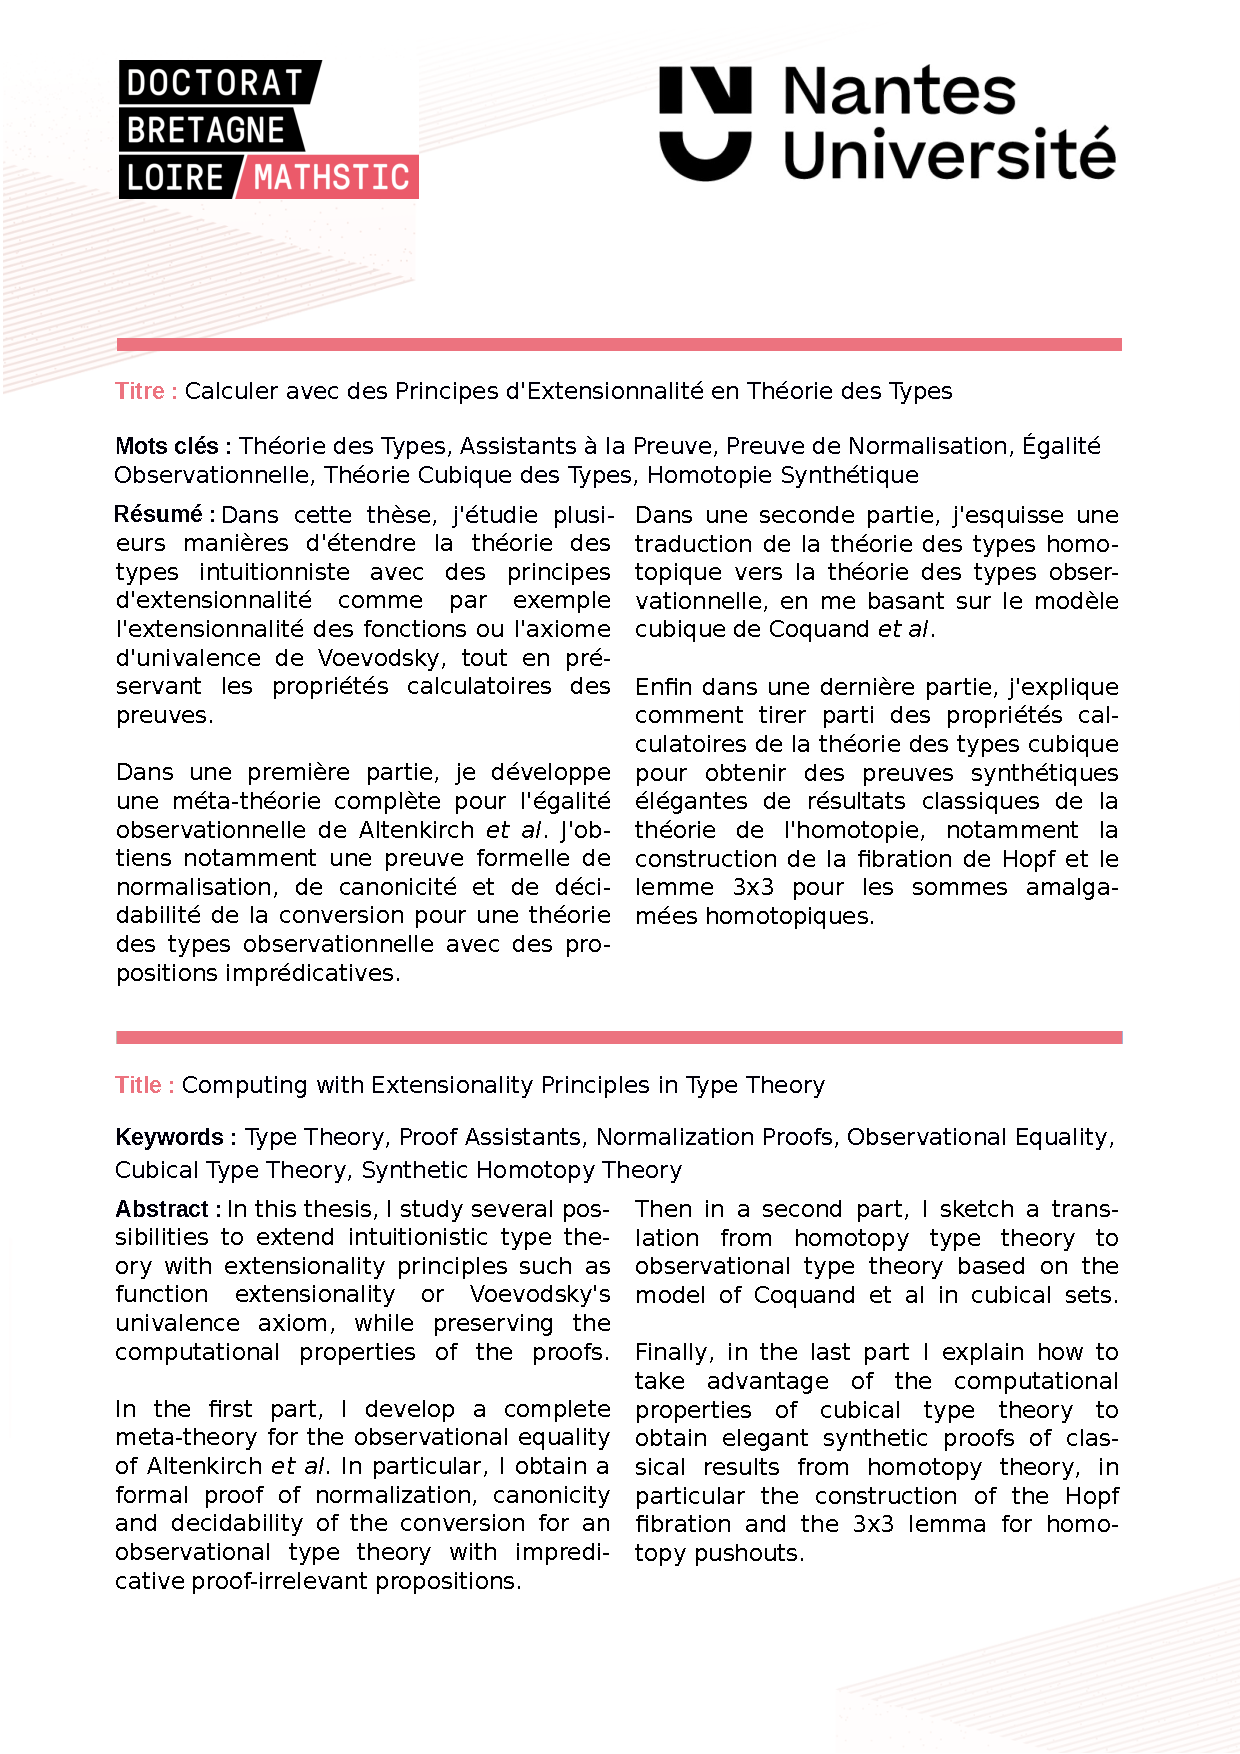
\includepdf{cover-back.pdf}

%----------------------------------------------------------------------------------------

\end{document}
